\documentclass[10pt,ngerman,aspectratio=169]{beamer}
\usepackage{lmodern}
\usepackage{amssymb,amsmath}
\usepackage{ifxetex,ifluatex}

\ifnum 0\ifxetex 1\fi\ifluatex 1\fi=0 % if pdftex
  \usepackage[T1]{fontenc}
  \usepackage[utf8]{inputenc}
\else % if luatex or xelatex
  \ifxetex
    \usepackage{mathspec}
  \else
    \usepackage{fontspec}
  \fi
  \defaultfontfeatures{Ligatures=TeX,Scale=MatchLowercase}
\fi
% use upquote if available, for straight quotes in verbatim environments
\IfFileExists{upquote.sty}{\usepackage{upquote}}{}
% use microtype if available
\IfFileExists{microtype.sty}{%
\usepackage{microtype}
\UseMicrotypeSet[protrusion]{basicmath} % disable protrusion for tt fonts
}{}
\usepackage{hyperref}
\PassOptionsToPackage{usenames,dvipsnames}{color} % color is loaded by hyperref
\hypersetup{unicode=true,
            pdftitle={Induktive Statistik},
            pdfauthor={Prof.~Dr.~Christoph Hanck},
            colorlinks=true,
            linkcolor=dueblue,
            citecolor=dueblue,
            urlcolor=dueblue,
            breaklinks=true}
\urlstyle{same}  % don't use monospace font for urls
\ifnum 0\ifxetex 1\fi\ifluatex 1\fi=0 % if pdftex
  \usepackage[shorthands=off,main=ngerman]{babel}
\else
  \usepackage{polyglossia}
  \setmainlanguage[]{}
\fi


\usepackage{color}
\usepackage{fancyvrb}
\newcommand{\VerbBar}{|}
\newcommand{\VERB}{\Verb[commandchars=\\\{\}]}
\DefineVerbatimEnvironment{Highlighting}{Verbatim}{commandchars=\\\{\}}
% Add ',fontsize=\small' for more characters per line
\usepackage{framed}
\definecolor{shadecolor}{RGB}{248,248,248}
\newenvironment{Shaded}{\begin{snugshade}}{\end{snugshade}}
\newcommand{\AlertTok}[1]{\textcolor[rgb]{0.94,0.16,0.16}{#1}}
\newcommand{\AnnotationTok}[1]{\textcolor[rgb]{0.56,0.35,0.01}{\textbf{\textit{#1}}}}
\newcommand{\AttributeTok}[1]{\textcolor[rgb]{0.13,0.29,0.53}{#1}}
\newcommand{\BaseNTok}[1]{\textcolor[rgb]{0.00,0.00,0.81}{#1}}
\newcommand{\BuiltInTok}[1]{#1}
\newcommand{\CharTok}[1]{\textcolor[rgb]{0.31,0.60,0.02}{#1}}
\newcommand{\CommentTok}[1]{\textcolor[rgb]{0.56,0.35,0.01}{\textit{#1}}}
\newcommand{\CommentVarTok}[1]{\textcolor[rgb]{0.56,0.35,0.01}{\textbf{\textit{#1}}}}
\newcommand{\ConstantTok}[1]{\textcolor[rgb]{0.56,0.35,0.01}{#1}}
\newcommand{\ControlFlowTok}[1]{\textcolor[rgb]{0.13,0.29,0.53}{\textbf{#1}}}
\newcommand{\DataTypeTok}[1]{\textcolor[rgb]{0.13,0.29,0.53}{#1}}
\newcommand{\DecValTok}[1]{\textcolor[rgb]{0.00,0.00,0.81}{#1}}
\newcommand{\DocumentationTok}[1]{\textcolor[rgb]{0.56,0.35,0.01}{\textbf{\textit{#1}}}}
\newcommand{\ErrorTok}[1]{\textcolor[rgb]{0.64,0.00,0.00}{\textbf{#1}}}
\newcommand{\ExtensionTok}[1]{#1}
\newcommand{\FloatTok}[1]{\textcolor[rgb]{0.00,0.00,0.81}{#1}}
\newcommand{\FunctionTok}[1]{\textcolor[rgb]{0.13,0.29,0.53}{\textbf{#1}}}
\newcommand{\ImportTok}[1]{#1}
\newcommand{\InformationTok}[1]{\textcolor[rgb]{0.56,0.35,0.01}{\textbf{\textit{#1}}}}
\newcommand{\KeywordTok}[1]{\textcolor[rgb]{0.13,0.29,0.53}{\textbf{#1}}}
\newcommand{\NormalTok}[1]{#1}
\newcommand{\OperatorTok}[1]{\textcolor[rgb]{0.81,0.36,0.00}{\textbf{#1}}}
\newcommand{\OtherTok}[1]{\textcolor[rgb]{0.56,0.35,0.01}{#1}}
\newcommand{\PreprocessorTok}[1]{\textcolor[rgb]{0.56,0.35,0.01}{\textit{#1}}}
\newcommand{\RegionMarkerTok}[1]{#1}
\newcommand{\SpecialCharTok}[1]{\textcolor[rgb]{0.81,0.36,0.00}{\textbf{#1}}}
\newcommand{\SpecialStringTok}[1]{\textcolor[rgb]{0.31,0.60,0.02}{#1}}
\newcommand{\StringTok}[1]{\textcolor[rgb]{0.31,0.60,0.02}{#1}}
\newcommand{\VariableTok}[1]{\textcolor[rgb]{0.00,0.00,0.00}{#1}}
\newcommand{\VerbatimStringTok}[1]{\textcolor[rgb]{0.31,0.60,0.02}{#1}}
\newcommand{\WarningTok}[1]{\textcolor[rgb]{0.56,0.35,0.01}{\textbf{\textit{#1}}}}
\usepackage{longtable,booktabs}
\IfFileExists{parskip.sty}{%
\usepackage{parskip}
}{% else
\setlength{\parindent}{0pt}
\setlength{\parskip}{3em plus 1pt minus 1pt}%{6pt plus 2pt minus 1pt}
}
\setlength{\emergencystretch}{3em}  % prevent overfull lines

\setcounter{secnumdepth}{0}
% Redefines (sub)paragraphs to behave more like sections
\ifx\paragraph\undefined\else
\let\oldparagraph\paragraph
\renewcommand{\paragraph}[1]{\oldparagraph{#1}\mbox{}}
\fi
\ifx\subparagraph\undefined\else
\let\oldsubparagraph\subparagraph
\renewcommand{\subparagraph}[1]{\oldsubparagraph{#1}\mbox{}}
\fi

%%% Use protect on footnotes to avoid problems with footnotes in titles
\let\rmarkdownfootnote\footnote%
\def\footnote{\protect\rmarkdownfootnote}


  \title{Induktive Statistik}
    \author{Prof.~Dr.~Christoph Hanck}
  
  \providecommand{\institute}[1]{}
  \expandafter\ifstrequal\expandafter{default}{default}{%
  \institute{\expandafter\ifstrequal\expandafter{de}{de}{%
  Universität Duisburg-Essen}{%
  University of Duisburg-Essen}}}{%
  
  \institute{default}
}


    \date{Sommersemester 2025}


% up until here https://github.com/rstudio/rmarkdown/blob/master/inst/rmd/latex/default-1.17.0.2.tex
%%%%%%%%%%%%%%%%%%%%%%%%%%%%%%%%%%%%%%%%%%%%%%%%%%%%%%%%%%%%%%%%%%%%%%%%%%%%%%%
%%% Additional packages
\makeatletter
\def\input@path{{"C:/Users/jens.klenke/AppData/Local/Programs/R/R-4.4.1/library/runidue/rmarkdown/templates/lectureslides/resources/"}}  % make them visible to tex to overcome warnings
\makeatother

%%This is style file ee.sty.
%%version 30/01/2002
%
\newcommand{\vnorm}[1]{\left|\!\left|#1\right|\!\right|}
%\newcommand{\lowexp}[1]{\raisebox{1.45mm}[-1.45mm]{\scriptsize{$#1$}}}
\newcommand{\lowexp}[2]{\raisebox{#2mm}[-#2mm]{\scriptsize{$#1$}}}
\newcommand{\newoperator}[3]{\newcommand*{#1}{\mathop{#2}#3}}
\newcommand{\renewoperator}[3]{\renewcommand*{#1}{\mathop{#2}#3}}
%
% symbols C,N,Q,R,Z for sets
\newcommand{\SC}{\mathbb{C}}
\newcommand{\SSS}{\mathbb{S}}
\newcommand{\SN}{\mathbb{N}}
\newcommand{\SQ}{\mathbb{Q}}
\newcommand{\SR}{\mathbb{R}}
\newcommand{\SZ}{\mathbb{Z}}
\newcommand{\SB}{\mathbb{B}}
%
% calligraphic capital letters
\newcommand{\calA}{\mathcal{A}}
\newcommand{\calB}{\mathcal{B}}
\newcommand{\calC}{\mathcal{C}}
\newcommand{\calD}{\mathcal{D}}
\newcommand{\calE}{\mathcal{E}}
\newcommand{\calF}{\mathcal{F}}
\newcommand{\calG}{\mathcal{G}}
\newcommand{\calH}{\mathcal{H}}
\newcommand{\calI}{\mathcal{I}}
\newcommand{\calJ}{\mathcal{J}}
\newcommand{\calK}{\mathcal{K}}
\newcommand{\calL}{\mathcal{L}}
\newcommand{\calM}{\mathcal{M}}
\newcommand{\calN}{\mathcal{N}}
\newcommand{\calO}{\mathcal{O}}
\newcommand{\calP}{\mathcal{P}}
\newcommand{\calQ}{\mathcal{Q}}
\newcommand{\calR}{\mathcal{R}}
\newcommand{\calS}{\mathcal{S}}
\newcommand{\calT}{\mathcal{T}}
\newcommand{\calU}{\mathcal{U}}
\newcommand{\calV}{\mathcal{V}}
\newcommand{\calW}{\mathcal{W}}
\newcommand{\calX}{\mathcal{X}}
\newcommand{\calY}{\mathcal{Y}}
\newcommand{\calZ}{\mathcal{Z}}
%
% bold lowercase and capital letters for vectors (v) and matrices (m)
\newcommand{\mA}{\bm A}
\newcommand{\va}{\bm a}
\newcommand{\mB}{\bm B}
\newcommand{\vb}{\bm b}
\newcommand{\mC}{\bm C}
\newcommand{\vc}{\bm c}
\newcommand{\mD}{\bm D}
\newcommand{\vd}{\bm d}
\newcommand{\mE}{\bm E}
\newcommand{\ve}{\bm e}
\newcommand{\mF}{\bm F}
\newcommand{\vf}{\bm f}
\newcommand{\mG}{\bm G}
\newcommand{\vg}{\bm g}
\newcommand{\mH}{\bm H}
\newcommand{\vh}{\bm h}
\newcommand{\mI}{\bm I}
\newcommand{\vi}{\bm i}
\newcommand{\mJ}{\bm J}
\newcommand{\vj}{\bm j}
\newcommand{\mK}{\bm K}
\newcommand{\vk}{\bm k}
\newcommand{\mL}{\bm L}
\newcommand{\vl}{\bm l}
\newcommand{\mM}{\bm M}
\newcommand{\vm}{\bm m}
\newcommand{\mN}{\bm N}
\newcommand{\vn}{\bm n}
\newcommand{\mO}{\bm O}
\newcommand{\vo}{\bm o}
\newcommand{\mP}{\bm P}
\newcommand{\vp}{\bm p}
\newcommand{\mQ}{\bm Q}
\newcommand{\vq}{\bm q}
\newcommand{\mR}{\bm R}
\newcommand{\vr}{\bm r}
\newcommand{\mS}{\bm S}
\newcommand{\vs}{\bm s}
\newcommand{\mT}{\bm T}
\newcommand{\vt}{\bm t}
\newcommand{\mU}{\bm U}
\newcommand{\vu}{\bm u}
\newcommand{\mV}{\bm V}
\newcommand{\vv}{\bm v}
\newcommand{\mW}{\bm W}
\newcommand{\vw}{\bm w}
\newcommand{\mX}{\bm X}
\newcommand{\vx}{\bm x}
\newcommand{\mY}{\bm Y}
\newcommand{\vy}{\bm y}
\newcommand{\mZ}{\bm Z}
\newcommand{\vz}{\bm z}
\newcommand{\vzero}{\bm 0}
\newcommand{\vone}{\bm 1}
%
% bold Greek lowercase letters for vectors (v)
\newcommand{\valpha}{\bm \alpha}
\newcommand{\vbeta}{\bm \beta}
\newcommand{\vgamma}{\bm \gamma}
\newcommand{\vdelta}{\bm \delta}
\newcommand{\vepsi}{\bm \epsi}
\newcommand{\vvarepsilon}{\bm \varepsilon}
\newcommand{\vzeta}{\bm \zeta}
\newcommand{\veta}{\bm \eta}
\newcommand{\vtheta}{\bm \theta}
\newcommand{\viota}{\bm \iota}
\newcommand{\vkappa}{\bm \kappa}
\newcommand{\vlambda}{\bm \lambda}
\newcommand{\vmu}{\bm \mu}
\newcommand{\vnu}{\bm \nu}
\newcommand{\vxi}{\bm \xi}
\newcommand{\vpi}{\bm \pi}
\newcommand{\vrho}{\bm \rho}
\newcommand{\vsigma}{\bm \sigma}
\newcommand{\vtau}{\bm \tau}
\newcommand{\vupsilon}{\bm \upsilon}
\newcommand{\vphi}{\bm \phi}
\newcommand{\vchi}{\bm \chi}
\newcommand{\vpsi}{\bm \psi}
\newcommand{\vomega}{\bm \omega}
%
% bold Greek capital letters for matrices (m)
\newcommand{\mGamma}{\bm \varGamma}
\newcommand{\mDelta}{\bm \varDelta}
\newcommand{\mTheta}{\bm \varTheta}
\newcommand{\mLambda}{\bm \varLambda}
\newcommand{\mXi}{\bm \varXi}
\newcommand{\mXib}{\bm \Xi}
\newcommand{\mPi}{\bm \varPi}
\newcommand{\mSigma}{\bm \varSigma}
\newcommand{\mUpsilon}{\bm \varUpsilon}
\newcommand{\mPhi}{\bm \varPhi}
\newcommand{\mPsi}{\bm \varPsi}
\newcommand{\mOmega}{\bm \varOmega}
%
% roman letters in mathematics
\newcommand{\rb}{\ensuremath{\mathrm{b}}}
\newcommand{\rB}{\ensuremath{\mathrm{B}}}
\newcommand{\rC}{\ensuremath{\mathrm{C}}}
\newcommand{\rD}{\ensuremath{\mathrm{D}}}
\newcommand{\rf}{\ensuremath{\mathrm{f}}}
\newcommand{\rF}{\ensuremath{\mathrm{F}}}
\newcommand{\rH}{\ensuremath{\mathrm{H}}}
\newcommand{\rL}{\ensuremath{\mathrm{L}}}
\newcommand{\rN}{\ensuremath{\mathrm{N}}}
\newcommand{\rt}{\ensuremath{\mathrm{t}}}
\newcommand{\rU}{\ensuremath{\mathrm{U}}}
\newcommand{\rGam}{\ensuremath{\mathrm{Gam}}}
\newcommand{\rBeta}{\ensuremath{\mathrm{Beta}}}
%
\newcommand{\Bin}{\ensuremath{\mathrm{Bin}}}
\newcommand{\eu}{\ensuremath{\mathrm{e}}}
\newcommand{\iu}{\ensuremath{\mathrm{i}}}
\newcommand{\LN}{\ensuremath{\mathrm{LN}}}
\newcommand{\IN}{\ensuremath{\mathrm{IN}}}

\newcommand{\Poi}{\ensuremath{\mathrm{Poi}}}
%
\newcommand{\ped}[1]{\ensuremath{_\mathrm{#1}}} %pedex
\newcommand{\ap}[1]{\ensuremath{^\mathrm{#1}}} %apex
\renewoperator{\Re}{\mathrm{Re}}{\nolimits}
\renewoperator{\Im}{\mathrm{Im}}{\nolimits}
%
% letters for (partial) differentiation
%\newcommand{\rd}{\ensuremath{\mathrm{d}}}
\makeatletter
\newcommand{\rd}{\@ifnextchar^{\DIfF}{\DIfF^{}}}
\def\DIfF^#1{%
   \mathop{\mathrm{\mathstrut d}}%
   \nolimits^{#1}\gobblespace}
\def\gobblespace{\futurelet\diffarg\opspace}
\def\opspace{%
   \let\DiffSpace\!%
   \ifx\diffarg(%
   \let\DiffSpace\relax
   \else
   \ifx\diffarg[%
   \let\DiffSpace\relax
   \else
   \ifx\diffarg\{%
   \let\DiffSpace\relax
   \fi\fi\fi\DiffSpace}
\newcommand{\deriv}[3][]{\frac{\rd^{#1}#2}{\rd #3^{#1}}}
\newcommand{\pderiv}[3][]{\frac{\partial^{#1}#2}{\partial #3^{#1}}}
%
% operatornames
\newcommand{\Avar}{\operatorname{Avar}}
\newcommand{\bias}{\operatorname{bias}}
\newcommand{\col}{\operatorname{col}}
\newcommand{\corr}{\operatorname{corr}}
\newcommand{\Corr}{\operatorname{Corr}}
\newcommand{\cov}{\operatorname{cov}}
\newcommand{\Cov}{\operatorname{Cov}}
\newcommand{\dg}{\operatorname{dg}}
\newcommand{\diag}{\operatorname{diag}}
\newcommand{\E}{\operatorname{E}}
\newcommand{\etr}{\operatorname{etr}}
\newoperator{\ip}{\mathrm{int}}{\nolimits}
\newcommand{\kur}{\operatorname{kur}}
%\newcommand{\median}{\operatorname{med}}
\newcommand{\MSE}{\operatorname{MSE}}
\newcommand{\plim}{\operatorname{plim}}
%\newcommand{\plim}{\DeclareMathOperator{plim}}
\newcommand{\cond}{\rightarrow_{\mathrm{d}}}
\newcommand{\conp}{\rightarrow_{\mathrm{p}}}
\newcommand{\rk}{\operatorname{rk}}
\newcommand{\sgn}{\operatorname{sgn}}
\newcommand{\spur}{\operatorname{spur}}
\newcommand{\tr}{\operatorname{tr}}
\newcommand{\var}{\operatorname{Var}}
\newcommand{\Var}{\operatorname{Var}}
\renewcommand{\vec}{\operatorname{vec}}
\newcommand{\vech}{\operatorname{vech}}
\DeclareMathOperator*{\argmin}{arg\,min}
\DeclareMathOperator*{\argmax}{arg\,max}
%
% other definitions
\newcommand{\distr}{\sim}
\newcommand{\adistr}{\stackrel{a}{\distr}}
\newcommand{\diff}{\Delta}
\newcommand{\fordiff}{\bigtriangleup}
\newcommand{\fdiff}{\diff_{\rf}}
\newcommand{\bdiff}{\diff_{\rb}}
%
%\mathchardef\varepsilon="010F
%\mathchardef\epsilon="0122
%\mathchardef\eps="010F
\newcommand{\eps}{\epsilon}
\newcommand{\epsi}{\varepsilon}
%
\newcommand{\longto}{\longrightarrow}
\newcommand{\pto}{\stackrel{p}{\longrightarrow}}
\newcommand{\dto}{\stackrel{d}{\longrightarrow}}
\newcommand{\wto}{\stackrel{w}{\longrightarrow}}
%
\newcommand{\Infmat}{\bm\calI}
\newcommand{\Hesmat}{\bm\calH}
\newcommand{\bcdot}{\raisebox{1pt}{\textbf{\large .}}}
\newcommand{\interior}[1]{\overset{\circ}{#1}}
%
\newcommand{\vones}{\bm\imath}
\newcommand{\vzeros}{\boldsymbol{0}}
\newcommand{\mZeros}{\mathbf{O}}
%
% additional commands
\newcommand{\EE}[1]{\E\left(#1\right)}
\renewcommand{\Pr}{\ensuremath{\mathrm{P}}}
\newcommand{\prob}[1]{\Pr\left(#1\right)}
\newcommand{\Prob}[1]{\Pr\left(#1\right)}
\newcommand{\Spur}[1]{\spur\left[#1\right]}
\newcommand{\vvarphi}{\bm \varphi}
%

\usepackage{BeamerColor}
\usepackage{hypernat}
\usepackage{mathtools}
\usepackage[export]{adjustbox}
\usepackage{makecell}
\usepackage{diagbox}
\usepackage{bm, bbm}
\usepackage{subfig}
\usepackage{forest}
\usepackage[labelfont={footnotesize,color=dueblue},font=footnotesize]{caption}
\usepackage{soul}
\usepackage{textcomp}
\usepackage{zref}
\usepackage{zref-user}
\usepackage{zref-xr}
\usepackage{empheq}
\usepackage{tikz}
\usetikzlibrary{arrows, decorations.markings}
\tikzstyle{arrow} = [ultra thick, - latex, shorten >= 2pt, shorten <= 2pt] % default arrow
\tikzstyle{vecArrow} = [thick, decoration={markings,mark=at position
	1 with {\arrow[semithick]{open triangle 60}}},
double distance=1.4pt, shorten >= 5.5pt,
preaction = {decorate},
postaction = {draw,line width=1.4pt, white,shorten >= 4.5pt}]
\tikzstyle{innerWhite} = [semithick, white,line width=1.4pt, shorten >= 4.5pt] % vec arrow
\tikzstyle{box} = [rectangle,rounded corners,fill=dueblue, text=white, align=center, node distance=1.25cm] % default node

% \usepackage{etoolbox}

\makeatletter
\let\@@magyar@captionfix\relax
\makeatother

%%% ZREF

%%% New colors
\definecolor{dueblue}{RGB}{0,76,147}
\definecolor{duelightblue}{RGB}{223,228,242}
\definecolor{duebeige}{RGB}{239,228,191}
\definecolor{darkgrey}{RGB}{40, 40, 40}
\definecolor{salmon}{RGB}{239, 148, 108}
\definecolor{lime}{RGB}{219, 254, 135}
\definecolor{sandy}{RGB}{255, 227, 129}
\definecolor{darklime}{RGB}{153, 194, 77}


%%% Additional commands
\newcommand{\npt}{\\[1ex]\pause}
\newcommand{\nbs}{\protect{~}}
\newcommand{\qedb}{\hfill \textsquare} % to be used outside proof environments
\newcommand{\pausealt}{ }
\newcommand{\blue}[1]{{\color{dueblue}{#1}\color{black}}}
\newcommand{\hil}[1]{\textbf{\color{dueblue}{#1}\color{black}}}
\newcommand{\hilm}[1]{\mathbf{\color{dueblue}{#1}\color{black}}}
\newcommand{\mps}{\par\medbreak}
\newcommand{\sd}{\operatorname{sd}}
\newcommand{\SD}{\operatorname{SD}}

% Kahoot Block
\newenvironment<>{kahoot}[1]{%
  \begin{actionenv}#2%
      \def\insertblocktitle{#1}%
      \par%
      \mode<presentation>{%
      \setbeamercolor{block title}{fg=black,bg=yellow}
       \setbeamercolor{block body}{fg=black,bg=yellow!20}
       \setbeamercolor{itemize item}{fg=orange!20!black}
       \setbeamertemplate{itemize item}[triangle]
     }%
      \usebeamertemplate{block begin}
      \begin{center}
\includegraphics[width=0.25\textwidth]{"C:/Users/jens.klenke/AppData/Local/Programs/R/R-4.4.1/library/runidue/rmarkdown/templates/lectureslides/resources/kahootlogo2"}
\end{center}}
    {\par\usebeamertemplate{block end}\end{actionenv}}
\newcommand{\kahootblock}[1]{\begin{kahoot}{#1}\end{kahoot}}

% QuizAcademy Block
\newenvironment<>{QuizAcademy}[1]{%
	\begin{actionenv}#2%
		\def\insertblocktitle{#1}%
		\par%
		\mode<presentation>{%
			\setbeamercolor{block title}{fg=black,bg=yellow}
			\setbeamercolor{block body}{fg=black,bg=yellow!20}
			\setbeamercolor{itemize item}{fg=orange!20!black}
			\setbeamertemplate{itemize item}[triangle]
		}%
		\usebeamertemplate{block begin}
		\begin{center}
			\includegraphics[width=0.25\textwidth]{"C:/Users/jens.klenke/AppData/Local/Programs/R/R-4.4.1/library/runidue/rmarkdown/templates/lectureslides/resources/QuizAcademy.png"}
	\end{center}}
	{\par\usebeamertemplate{block end}\end{actionenv}}
\newcommand{\QuizAcademyblock}[1]{\begin{QuizAcademy}{#1}\end{QuizAcademy}}



% Rlogo
\makeatletter
\newcommand*\fsize{\dimexpr\f@size pt\relax} % returns current font size
\makeatother
\newcommand{\R}{\includegraphics[height=.85\fsize, clip=T]{"C:/Users/jens.klenke/AppData/Local/Programs/R/R-4.4.1/library/runidue/rmarkdown/templates/lectureslides/resources/Rlogo"}\ }
\newcommand{\btVFill}{\vskip0pt plus 1filll}
\newcommand{\source}[1]{\btVFill\scriptsize \textit{\expandafter\ifstrequal\expandafter{de}{de}{Quelle: }{Source: }}#1}



% BLOCK ENVIRONMENTS (THEOREMS)
\expandafter\ifstrequal\expandafter{box}{blank}{
}{
\setbeamerfont{block title}{size=\normalsize}
\setbeamercolor{block title}{bg=duelightblue,fg=black}
\setbeamercolor{block body}{bg=duelightblue!37,fg=black}
}%
\setbeamertemplate{blocks}[rounded][shadow=false]

% Headers for theorems
\expandafter\ifstrequal\expandafter{de}{de}{%
  \newcommand{\thmncont}{Fortsetzung}
  \newtheorem{thmn}{Theorem}[section]
  \newtheorem{lem}[thmn]{Lemma}
  \newtheorem{cor}[thmn]{Corollary}
  \newtheorem{defn}[thmn]{Definition}
  \newtheorem{ass}[thmn]{Annahme}
  \newtheorem{rem}[thmn]{Anmerkung}
  \newtheorem{prop}[thmn]{Proposition}
  \theoremstyle{definition}
  \newtheorem{xmpl}[thmn]{Beispiel}
  \newtheorem{que}[thmn]{Frage}
  \newtheorem{exe}[thmn]{Aufgabe}
  \numberwithin{equation}{section}}{%%%
  \newcommand{\thmncont}{Continued}
  \newtheorem{thmn}{Theorem}[section]
  \newtheorem{lem}[thmn]{Lemma}
  \newtheorem{cor}[thmn]{Corollary}
  \newtheorem{defn}[thmn]{Definition}
  \newtheorem{ass}[thmn]{Assumption}
  \newtheorem{rem}[thmn]{Remark}
  \newtheorem{prop}[thmn]{Proposition}
  \theoremstyle{definition}
  \newtheorem{xmpl}[thmn]{Example}
  \newtheorem{que}[thmn]{Question}
  \newtheorem{exe}[thmn]{Exercise}
  \numberwithin{equation}{section}
}%

% CONTINUING BLOCKS
\newenvironment{thmn*}{\addtocounter{thmn}{-1}\thmn[\thmncont]}{\endthmn}
\newenvironment{lem*}{\addtocounter{thmn}{-1}\lem[\thmncont]}{\endlem}
\newenvironment{cor*}{\addtocounter{thmn}{-1}\cor[\thmncont]}{\endcor}
\newenvironment{defn*}{\addtocounter{thmn}{-1}\thmn[\thmncont]}{\endthmn}
\newenvironment{ass*}{\addtocounter{thmn}{-1}\ass[\thmncont]}{\endass}
\newenvironment{rem*}{\addtocounter{thmn}{-1}\rem[\thmncont]}{\endrem}
\newenvironment{xmpl*}{\addtocounter{thmn}{-1}\xmpl[\thmncont]}{\endxmpl}
\newenvironment{que*}{\addtocounter{thmn}{-1}\que[\thmncont]}{\endque}


\setbeamertemplate{theorems}[numbered]
\setbeamerfont{block title}{size=\normalsize}
\setbeamertemplate{theorem begin}
{%
  \expandafter\ifstrequal\expandafter{\inserttheoremaddition}{*}{\addtocounter{thmn}{-1}}{}
  \normalfont
  \begin{\inserttheoremblockenv}{%
    \structure{%
      \textcolor{darkgrey}{\textbf{\inserttheoremname \inserttheoremnumber}:
      \ifx\inserttheoremaddition\empty\else\expandafter\ifstrequal\expandafter{\inserttheoremaddition}{*}{\thmncont\inserttheorempunctuation}{\inserttheoremaddition\inserttheorempunctuation}\fi}%
    }%
  }%
}
\setbeamertemplate{theorem end}{\leavevmode\end{\inserttheoremblockenv}}

\preto{\xmpl}{
    \setbeamercolor{block title}{fg=black,bg=sandy!70!white}
    \setbeamercolor{block body}{fg=black, bg=sandy!20!white}
}

\preto{\exe}{
    \setbeamercolor{block title}{fg=black,bg=darklime!70!white}
    \setbeamercolor{block body}{fg=black, bg=darklime!20!white}
}




% Spacings
\AtBeginEnvironment{figure}{\setlength{\parskip}{-2ex}}
\AtBeginEnvironment{center}{\smallbreak}
\AtEndEnvironment{center}{\smallbreak}
\AtBeginEnvironment{itemize}{\smallskip \setlength{\itemsep}{0.3ex}\setlength{\parskip}{1ex}}
\AtEndEnvironment{itemize}{\smallskip}
\preto{\enumerate}{\medskip  \setlength{\itemsep}{0.75ex}\setlength{\parskip}{1ex}}
\AtEndEnvironment{enumerate}{\smallskip}



% \let\tempone\itemize
% \let\temptwo\enditemize
% \renewenvironment{itemize}{\tempone\setlength{\itemsep}{1ex}\setlength{\parskip}{1.2ex}}{\temptwo}

% \let\tempone\enumerate
% \let\temptwo\endenumerate
% \renewenvironment{enumerate}{\tempone\setlength{\itemsep}{1ex}\setlength{\parskip}{1.2ex}}{\temptwo}
% 




%%% LAYOUT
\usecolortheme[named=dueblue]{structure}
\beamertemplatenavigationsymbolsempty
\setbeamersize{text margin left=10pt, text margin right=10pt}


% Spacing before and after code chunks / output
\makeatletter
\preto{\@verbatim}{\topsep=-2pt \partopsep=2pt \parskip=-2ex}
\makeatother

% spacing before figure captions
\setlength{\abovecaptionskip}{0pt}
\setlength{\belowcaptionskip}{-1em plus 1em minus 0em}

% spacing aorund display equations
\setlength{\abovedisplayskip}{3pt}
%\setlength{\belowdisplayskip}{3pt}

 % 

% Frame Head
\makeatletter
\setbeamertemplate{frametitle}{%
\vspace{.1cm}
\begin{minipage}[t][1cm]{1\textwidth}
    \ifbeamer@plainframe%
      \Large\insertframetitle%
    \else
      \Large\insertframetitle%
      \hfill
      \includegraphics[width=2cm,keepaspectratio=true, valign=t]{"C:/Users/jens.klenke/AppData/Local/Programs/R/R-4.4.1/library/runidue/rmarkdown/templates/lectureslides/resources/duelogo"} 
      \ifx\insertframesubtitle\empty
      \else
        \\ \small \insertframesubtitle
      \fi
    \fi
\end{minipage}

}
\makeatother

%%\includegraphics[width=2cm,keepaspectratio=true, valign=t]{"C:/Users/jens.klenke/AppData/Local/Programs/R/R-4.4.1/library/runidue/rmarkdown/templates/lectureslides/resources/duelogo"}
%    





% Footer
\setbeamercolor{footlinecolor}{bg=dueblue,fg=white}


\ifstrequal{default}{colored}{
\setbeamertemplate{footline}{
  % \hbox{
  \begin{beamercolorbox}[wd=\paperwidth,ht=0.4cm, leftskip=0cm, rightskip=0cm]{footlinecolor}
    \hfill \scriptsize{{\insertshortauthor : }
    \insertshorttitle---\insertsection \hfill \thesection-\insertframenumber\hspace*{.15cm}}\vspace{1mm}
  \end{beamercolorbox}
  % }
}
\addtobeamertemplate{footline}{\hypersetup{linkcolor=.}}{}
}{
\setbeamertemplate{footline}{\hspace*{.1cm}%
\hfill \scriptsize{{\insertshortauthor : }
\insertshorttitle---\insertsection \hfill \thesection-\insertframenumber\hspace*{.2cm}}\vspace{1mm}}
}




% TOC


\setbeamertemplate{section in toc shaded}[default][50]
\defbeamertemplate{section in toc}{customcircle}
{\leavevmode\leftskip=4ex%
  \llap{%
    \usebeamerfont*{section number projected}%
    \usebeamercolor{section number projected}%
    \begin{pgfpicture}{-1ex}{-.2ex}{1ex}{2ex}
      \color{bg}
      \pgfpathcircle{\pgfpoint{0pt}{.75ex}}{1.3ex}
      \pgfusepath{fill}
      \pgftext[base]{\color{fg}\inserttocsectionnumber}
    \end{pgfpicture}\kern1.25ex%
  }%
  \hspace{0.8ex}\inserttocsection\par}

\setbeamertemplate{section in toc}[customcircle]

% \usepackage{xpatch}
% \xpatchcmd{\itemize}
%   {\def\makelabel}
%   {\setlength{\itemsep}{1ex}\def\makelabel}
%   {}
%   {}
% \makeatletter
% \xpatchcmd{\beamer@enum@}
%   {\def\makelabel}
%   {\setlength{\itemsep}{1ex}\def\makelabel}
%   {}
%   {}
% \makeatother

% NEW SECTION


\AtBeginSection[] {
{
\setbeamertemplate{footline}{}
\begin{frame}{\expandafter\ifstrequal\expandafter{de}{de}{Überblick}{Outline}}
\vspace{0.5cm}
\tableofcontents[currentsection]
\end{frame}
\addtocounter{framenumber}{-\insertframenumber} % collect all begin section commands in one env.!
}
}

% ITEMIZE, ENUMERATE, DESCRIPTION
\defbeamertemplate*{description item}{defaultperiod}{\insertdescriptionitem.}
\setbeamersize{description width=15pt} % left margin for description

\setlength{\topsep}{1ex}
\setlength{\leftmargini}{10pt+.5\labelwidth}
\setlength{\leftmarginii}{15pt}
\setlength{\leftmarginiii}{15pt}


\setbeamertemplate{caption}[numbered]
\setbeamertemplate{caption label separator}{: }
\setbeamertemplate{itemize item}[circle]
\setbeamertemplate{itemize subitem}[triangle]
\setbeamertemplate{enumerate item}[default]
\setbeamertemplate{enumerate subitem}[default]
\setbeamertemplate{description item}[defaultperiod]
\setbeamertemplate{description subitem}[defaultperiod]


\providecommand{\tightlist}{}% \setlength{\itemsep}{0.75ex}\setlength{\parskip}{1.2ex}
% allow environments inside environments
\let\otherbegin\begin
\let\otherend\end
%%%%%%%%%%%%%%%%%%%%%%%%%%%%%%%%%%%%%%%%%%%%%%%%%%%%%%%%%%%%%%%%%%%%%%%%%%%%%%%
% from here on https://github.com/rstudio/rmarkdown/blob/master/inst/rmd/latex/default-1.17.0.2.tex



\begin{document}


      {\usebackgroundtemplate{\includegraphics[scale=0.25]{"C:/Users/jens.klenke/AppData/Local/Programs/R/R-4.4.1/library/runidue/rmarkdown/templates/lectureslides/resources/duetower"}}
    \frame[plain]{\titlepage}}
  

% 
\section{Einleitung}\label{einleitung}

\begin{frame}{Motivation}
\phantomsection\label{motivation}
\begin{itemize}
\tightlist
\item
  Ziel der \hil{deskriptiven} (beschreibenden) \hil{Statistik}: das
  Datenmaterial mit Hilfe tabellarischer und grafischer Repräsentationen
  sowie geeigneter Kenngrößen übersichtlich aufbereiten.
\item
  Ziel der \hil{induktiven} (schließenden) \hil{Statistik}: Verifikation
  theoretischer Modelle anhand von Daten und Testen von Hypothesen über
  unbekannte Parameter auf Basis von Wahrscheinlichkeitsmodellen.
\end{itemize}
\end{frame}

\begin{frame}{Motivation}
\phantomsection\label{motivation-1}
\framesubtitle{Beispiel: Lernerfolg}

\footnotesize
\begin{center}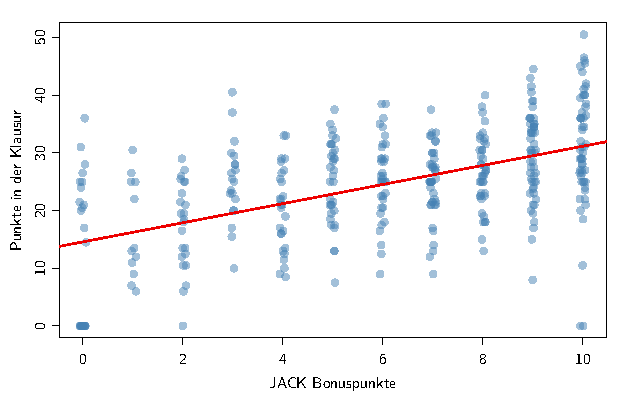
\includegraphics{Resources/Plots/unnamed-chunk-2-1} \end{center}
\normalsize
\end{frame}

\begin{frame}{Motivation}
\phantomsection\label{motivation-2}
Übergang von der deskriptiven zur induktiven Statistik:

\begin{itemize}
\tightlist
\item
  \hil{Induktives Schließen}, statistische Inferenz,
  Repräsentationsschluss: Schluss von einer Teilgesamtheit auf die
  Grundgesamtheit
\item
  \hil{Induktive Statistik}: Methoden, die es erlauben von den
  Beobachtungen einer Teilgesamtheit \linebreak (= \emph{Stichprobe})
  auf bestimmte Charakteristika der dazugehörenden
  \emph{Grundgesamtheit} zu schließen.
\end{itemize}
\end{frame}

\begin{frame}{Motivation}
\phantomsection\label{motivation-3}
\begin{itemize}
\tightlist
\item
  Beim Glücksspiel meinen Sie, dass die \glqq{}Gegenseite\grqq{} mit
  manipulierten Würfeln spielt, d.h. die Zahl 6 fällt häufiger als
  andere Zahlen. Wie können Sie Ihre Vermutung überprüfen?
\item
  Vor der Bundestagswahl prognostiziert ein Wahlforschungsinstitut, dass
  30\% der Stimmen auf die CDU/CSU entfallen. Wie kann eine solche
  Prognose verlässlich durchgeführt werden?
\end{itemize}

Ziel: Schlussfolgerungen von einer Stichprobe auf die Grundgesamtheit
\end{frame}

\begin{frame}{Motivation}
\phantomsection\label{motivation-4}
\framesubtitle{QuizAcademy}

\QuizAcademy{Schokoladenwürfel}\endQuizAcademy
\end{frame}

\begin{frame}{Motivation}
\phantomsection\label{motivation-5}
\begin{center}
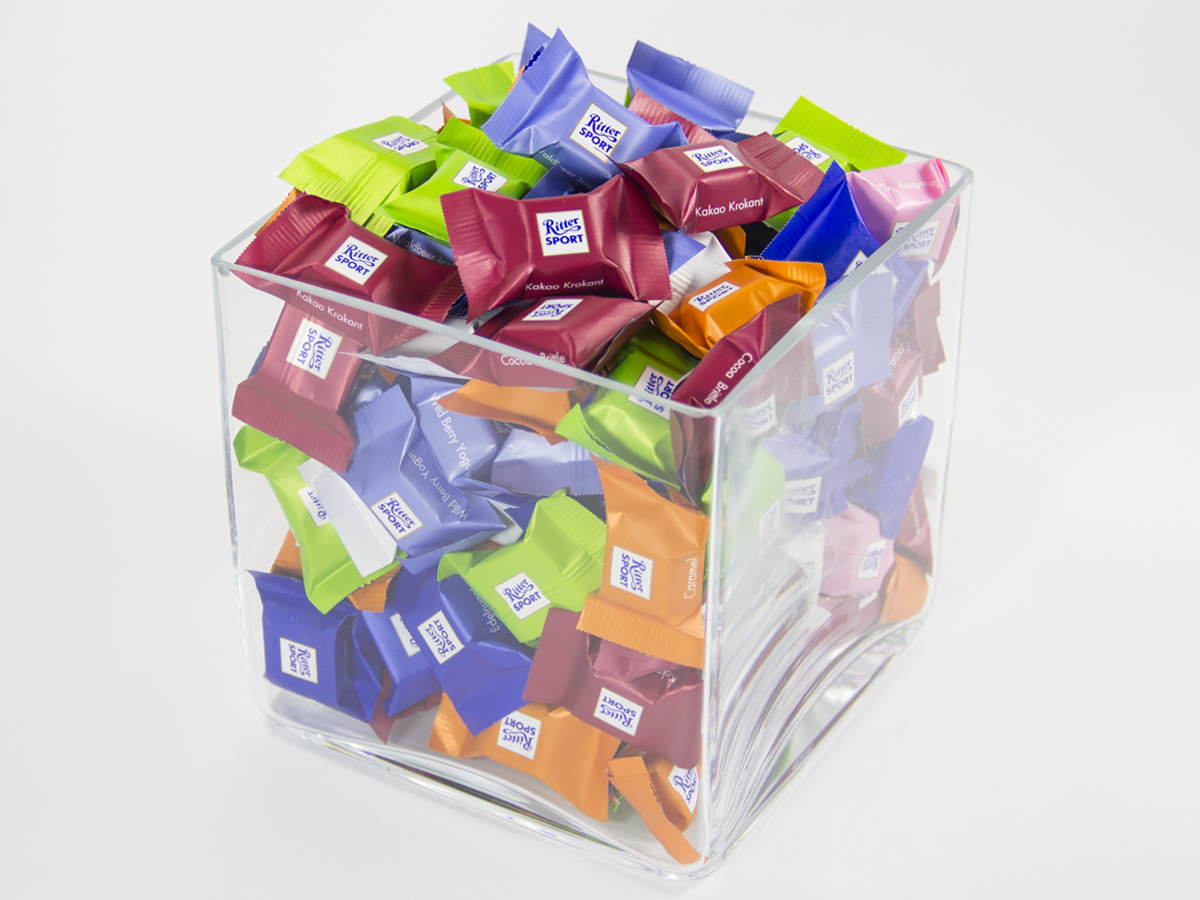
\includegraphics[height=0.6\textheight, keepaspectratio]{Resources/Grafiken/Schaetzen.jpg}
\end{center}
\source{\href{https://blog.ritter-sport.de/2014/08/05/schatzt-euch-bunt/}{https://blog.ritter-sport.de/2014/08/05/schatzt-euch-bunt/}}
\end{frame}

\begin{frame}{Motivation}
\phantomsection\label{motivation-6}
Man beachte: Wahrscheinlichkeitsrechnung

\begin{itemize}
\tightlist
\item
  ist \textbf{mehr} als Grundlage der schließenden Statistik
\item
  hat enorme eigenständige ökonomische Bedeutung z.B. in

  \begin{itemize}
  \tightlist
  \item
    Mikroökonomik
  \item
    Investition und Finanzierung
  \item
    Portfoliotheorie
  \end{itemize}
\end{itemize}
\end{frame}

\begin{frame}{Gliederung}
\phantomsection\label{gliederung}
\begin{enumerate}
\tightlist
\item
  Einleitung
\item
  Grundlagen
\item
  Eindimensionale Zufallsvariablen
\item
  Ausgewählte theoretische Verteilungen
\item
  Grundzüge der Stichprobentheorie
\item
  Statistische Schätzverfahren
\item
  Statistische Testverfahren
\item
  Zweidimensionale Zufallsvariablen
\end{enumerate}
\end{frame}

\section{Grundlagen}\label{grundlagen}

\begin{frame}{Grundlegende Begriffe}
\phantomsection\label{grundlegende-begriffe}
\framesubtitle{Zufallsvorgang}

Zufallsvorgänge (bzw. stochastische Vorgänge) sind durch zwei
wesentliche Eigenschaften gekennzeichnet:

\begin{enumerate}
\tightlist
\item
  Sie besitzen verschiedene, sich gegenseitig ausschließende Ausgänge,
  die bereits vor Beginn des Vorgangs bekannt sind;
\item
  es ist nicht vorhersehbar, welcher Ausgang tatsächlich eintreten wird.
\end{enumerate}

\hil{Beispiele} für Zufallsvorgänge:

\begin{itemize}
\tightlist
\item
  Der Ausgang eines Fußballspiels, der Kurs einer Aktie am nächsten Tag
  oder die realisierte Augenzahl eines Würfelwurfes.
\end{itemize}
\end{frame}

\begin{frame}{Grundlegende Begriffe}
\phantomsection\label{grundlegende-begriffe-1}
\framesubtitle{Zufallsvorgang, Zufallsexperiment}

\begin{itemize}
\tightlist
\item
  Ist ein Zufallsvorgang unverändert beliebig oft wiederholbar, liegt
  ein \hil{Zufallsexperiment} vor. Die unveränderte Wiederholbarkeit
  beschreibt man auch als unter gleichen (Rand-)Bedingungen
  wiederholbar.
\item
  D.h., dass die Randbedingungen wie bei naturwissenschaftlichen
  Experimenten kontrolliert werden können. Dies stellt sicher, dass die
  Bedingungen, unter denen das Experiment stattgefunden hat, auch bei
  weiteren Durchführungen hätten eingehalten werden können.
\item
  Damit gehören alle Zufallsvorgänge, die fiktiv unter gleichen
  Bedingungen wiederholbar sind, zu den Zufallsexperimenten. Dies
  erlaubt es, auch Zufallsvorgänge als Zufallsexperimente aufzufassen,
  deren praktische Wiederholung unter gleichen Bedingungen schwierig
  wäre.
\end{itemize}
\end{frame}

\begin{frame}{Grundlegende Begriffe}
\phantomsection\label{grundlegende-begriffe-2}
\framesubtitle{Zufallsvorgang, Zufallsexperiment, Stichprobenraum}

\begin{itemize}
\tightlist
\item
  Alle Ausgänge \(\omega_i\) eines Zufallsvorganges bzw. -experimentes
  fasst man zu einem \hil{Stichprobenraum} (Ergebnis- bzw. Ereignisraum)
  \(\Omega\) zusammen. Der Stichprobenraum ist eine Menge, deren
  Elemente die Ausgänge sind.
\item
  \(\Omega\) kann endlich oder unendlich viele Ausgänge enthalten.
  Lassen sich die unendlich vielen Ausgänge mit den natürlichen Zahlen
  \(\mathbb{N}\) abzählen, bezeichnet man \(\Omega\) als
  \hil{abzählbar unendlich}. Gelingt dies nicht, heißt \(\Omega\)
  \hil{überabzählbar unendlich}.
\end{itemize}

\[\Omega=\{\omega_1,\ldots,\omega_m,\ldots\}.\]
\end{frame}

\begin{frame}{Grundlegende Begriffe}
\phantomsection\label{grundlegende-begriffe-3}
\framesubtitle{Zufallsvorgang, Zufallsexperiment, Stichprobenraum}

\xmpl[Würfelwurf]Der Zufallsvorgang \emph{Werfen eines Würfels} hat
sechs mögliche Ausgänge.

\(\Omega\) ist endlich und lässt sich schreiben als:
\[ \Omega=\{\omega_1,\omega_2,\ldots,\omega_6\}=\{\omega_i,i=1,\ldots,6\} =\{1,2,3,4,5,6\}. \]
\endxmpl
\end{frame}

\begin{frame}{Grundlegende Begriffe}
\phantomsection\label{grundlegende-begriffe-4}
\framesubtitle{Zufallsvorgang, Zufallsexperiment, Stichprobenraum}

\xmpl[Münzwurf]Wirft man eine Münze mit Seiten \emph{Zahl} \((Z)\) und
\emph{Kopf} \((K)\) bis zum ersten Mal \(Z\) erscheint, lauten die
möglichen Ausgänge: \begin{alignat*}{2}
\omega_1&=Z&\qquad &\text{(zum ersten Mal \textit{Zahl} im ersten Wurf),}\\
\omega_2&=KZ&\qquad &\text{(zum ersten Mal \textit{Zahl} im zweiten Wurf),}\\
\vdots&&\qquad&\\
\omega_m&=\underset{m-1}{\underbrace{K\ldots K}}Z&\qquad &\text{(zum ersten Mal \textit{Zahl} im $m$--ten Wurf),}\\
\vdots&&\qquad&
\end{alignat*} Der Stichprobenraum ist hier abzählbar unendlich:
\vspace{-0.75em} \[\Omega=\{\omega_1,\ldots\omega_m,\ldots\}\,.\]
\endxmpl
\end{frame}

\begin{frame}{Grundlegende Begriffe}
\phantomsection\label{grundlegende-begriffe-5}
\framesubtitle{Zufallsvorgang, Zufallsexperiment, Stichprobenraum}

\xmpl[Zugverspätung]Die Verspätung eines Zuges in Minuten sei ein
Zufallsvorgang mit Ausgängen im Intervall \([0; 10]\). Bei unendlicher
Messgenauigkeit sind überabzählbar viele Verspätungen möglich, da das
Intervall \([0; 10]\) Teilmenge der reellen Zahlen \(\mathbb{R}\) ist.

Die reellen Zahlen sind, wie auch jede ihrer Teilmengen, mächtiger als
\(\mathbb{N}\) und daher überabzählbar unendlich. \endxmpl
\end{frame}

\begin{frame}{Grundlegende Begriffe}
\phantomsection\label{grundlegende-begriffe-6}
\framesubtitle{Ereignisse}

\begin{itemize}
\tightlist
\item
  Jede Teilmenge von \(\Omega\) heißt \hil{(Zufalls--)Ereignis}.
\item
  Da eine Menge auch Teilmenge von sich selbst und die leere Menge
  \(\emptyset\) Teilmenge jeder Menge ist, sind \(\Omega\) und
  \(\emptyset\) selbst Ereignisse von \(\Omega\).
\item
  Ein Ereignis \(A \subset \Omega\) tritt ein, wenn der Ausgang
  \(\omega_i\) des Zufallsvorgangs Element von \(A\) ist:
  \(\omega_i\in A\).
\item
  Da ein Zufallsvorgang immer in einem Ausgang \(\omega_i\in\Omega\)
  mündet, ist \(\Omega\) auch das \hil{sichere Ereignis}.
\item
  Analog hierzu heißt die leere Menge \(\emptyset\) das
  \hil{unmögliche Ereignis}, weil kein \(\omega_i\in\Omega\) existiert,
  das Element der leeren Menge \(\emptyset\) ist:
  \(\omega_i\notin \emptyset, i=1,\ldots,m\).
\end{itemize}
\end{frame}

\begin{frame}{Grundlegende Begriffe}
\phantomsection\label{grundlegende-begriffe-7}
\framesubtitle{Ereignisse}

\begin{itemize}
\tightlist
\item
  Teilmengen \(\{\omega_i\}\), deren einziges Element ein Ausgang
  \(\omega_i\in\Omega\) ist, heißen \hil{Elementarereignisse}.
\item
  Umfassen Teilmengen mehrere Ausgänge, nennt man sie
  \hil{zusammengesetzte Ereignisse}.
\item
  Z.\nbs B. ist beim \emph{\blue{Wurf eines Würfels}} der Ausgang:
  \emph{\blue{Augenzahl 3 liegt oben}} ein Elementarereignis und wird
  geschrieben als \(\{3\}\); das Ereignis \(A\):
  \emph{\blue{gerade Augenzahl liegt oben}} ist ein zusammengesetztes
  Ereignis, als Menge geschrieben: \(\{2,4,6\}\).
\item
  \(A\) tritt ein, wenn der Würfelwurf die Augenzahl 2, 4 oder 6 ergibt.
\end{itemize}
\end{frame}

\begin{frame}{Grundlegende Begriffe}
\phantomsection\label{grundlegende-begriffe-8}
\framesubtitle{Ereignisse}

\begin{itemize}
\tightlist
\item
  Die insgesamt möglichen Ereignisse eines Zufallsvorgangs findet man,
  indem alle Teilmengen für \(\Omega\) gebildet werden.
\item
  Die Zusammenfassung dieser Teilmengen führt bei endlichem oder
  abzählbar unendlichem Stichprobenraum \(\Omega\) zur \hil{Potenzmenge}
  \(PM(\Omega)\).
\item
  Die Anzahl der Ereignisse der Potenzmenge ist \(2^m\), wobei m der
  Anzahl der Elemente von \(\Omega\) entspricht.
\item
  Siehe Buch, S.\nbs 11.
\end{itemize}
\end{frame}

\begin{frame}{Grundlegende Begriffe}
\phantomsection\label{grundlegende-begriffe-9}
\framesubtitle{Ereignisse}

\xmpl[Potenzmenge]\label{xmpl:potenz} Ein Zufallsvorgang hat den
Stichprobenraum \(\Omega=\{1,2,3\}\); wegen \(m=3\) beträgt die Anzahl
der möglichen Ereignisse \[2^3=8.\] Diese Ereignisse lauten
\(A_1=\emptyset\), \(A_2=\{1\}\), \(A_3=\{2\}\), \(A_4=\{3\}\),
\(A_5=\{1,2\}\), \(A_6=\{1,3\}\), \(A_7=\{2,3\}\),
\(A_8=\{1,2,3\}=\Omega\). Die Potenzmenge ist
\[PM(\Omega)=\{A_1,\ldots,A_8\}.\] \endxmpl
\end{frame}

\begin{frame}{Grundlegende Begriffe}
\phantomsection\label{grundlegende-begriffe-10}
\framesubtitle{Vereinigungsereignis}

\begin{itemize}
\tightlist
\item
  Zwischen den Ereignissen können bestimmte Beziehungen vorliegen.
\item
  \blue{Beispiel:} Das Ereignis \(A_5 =\{1,2\}\) tritt dann ein, wenn
  entweder \(A_2=\{1\}\) oder \(A_3=\{2\}\) eintritt. \(A_5\) heißt
  daher \hil{Vereinigungsereignis}, geschrieben als
  \(A_5 = A_2\cup A_3\).
\item
  Verallgemeinert erhält man Vereinigungsereignisse \(V\) als
  \(V=\bigcup^n_{j=1}A_j\).
\item
  Für \(n=2\) ist \(V\) als rote Fläche im \hil{Venn--Diagramm}
  wiedergegeben, wobei das Rechteck den Stichprobenraum \(\Omega\)
  festlegt.
\end{itemize}

\vspace{-0.5cm}

\footnotesize
\begin{center}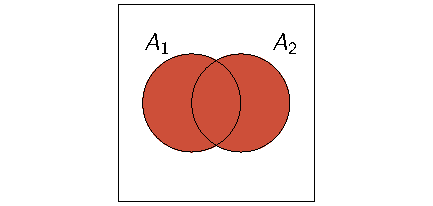
\includegraphics{Resources/Plots/Vereinigung-1} \end{center}
\normalsize
\end{frame}

\begin{frame}{Grundlegende Begriffe}
\phantomsection\label{grundlegende-begriffe-11}
\framesubtitle{Durchschnittsereignis}

\begin{itemize}
\tightlist
\item
  Ist der Schnitt zweier Ereignisse \(A_i\) und \(A_j\) nicht leer, gilt
  \(A_i\cap A_j=D\neq\emptyset\), so treten mit \(D\) auch die
  Ereignisse \(A_i\) und \(A_j\) ein.
\item
  \(D\) heißt daher \hil{Durchschnittsereignis}, das allgemein definiert
  ist als \(D=\bigcap_{j=1}^n A_j\). \(D\) tritt ein, wenn alle \(A_j\)
  eintreten.
\end{itemize}

\vspace{-0.5cm}

\footnotesize
\begin{center}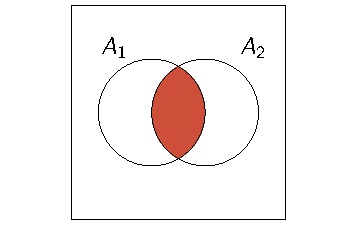
\includegraphics{Resources/Plots/Durchschnitt-1} \end{center}
\normalsize
\end{frame}

\begin{frame}{Grundlegende Begriffe}
\phantomsection\label{grundlegende-begriffe-12}
\framesubtitle{Komplementärereignis}

\begin{itemize}
\tightlist
\item
  Tritt \(A_i\) genau dann ein, wenn \(A_j\) nicht eintritt, so sind die
  beiden Ereignisse zueinander komplementär.
\item
  \(A_i\) heißt \hil{Komplementärereignis} oder kurz Komplement und
  lässt sich schreiben als \(A_i=\bar{A}_j\). Natürlich ist auch \(A_j\)
  Komplementärereignis zu \(A_i\): \(A_j = \bar{A}_i\).
\item
  Im Beispiel \ref{xmpl:potenz} ist das Ereignis \(A_2=\{1\}\) das
  Komplement zu \(A_7 =\{2,3\}:A_2=\bar{A}_7.\) Umgekehrt gilt auch
  \(A_7=\bar{A}_2\).
\item
  Für \(A\) und sein Komplement \(\bar{A}\) gelten
  \(A \cup \bar{A} = \Omega\) und \(A \cap \bar{A} = \emptyset\).
\end{itemize}

\footnotesize
\begin{center}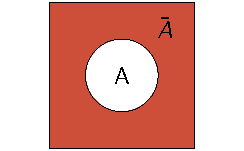
\includegraphics{Resources/Plots/Komplementaerereignis-1} \end{center}
\normalsize
\end{frame}

\begin{frame}{Grundlegende Begriffe}
\phantomsection\label{grundlegende-begriffe-13}
\framesubtitle{Teilereignisse und disjunkte Ereignisse}

\begin{itemize}
\tightlist
\item
  \(A_i\) und \(A_j\) heißen \hil{disjunkt}, wenn ihr Schnitt leer ist:
  \(A_i\cap A_j =\emptyset\).
\item
  Komplementäre Ereignisse sind daher immer auch disjunkt, die Umkehrung
  gilt aber nicht.
\item
  So sind im Beispiel \ref{xmpl:potenz} \(A_2=\{1\}\) und
  \(A_3 = \{2\}\) zwar disjunkt, aber nicht komplementär. Denn wenn
  \(A_3\) nicht eintritt, folgt nicht notwendigerweise das Eintreten von
  \(A_2\); es könnte auch \(A_4=\{3\}\) eintreten.
\end{itemize}

\footnotesize
\begin{center}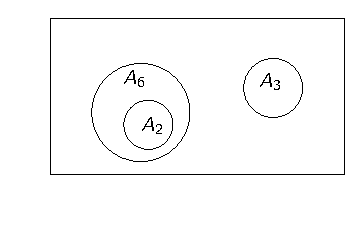
\includegraphics{Resources/Plots/Disjunkt-1} \end{center}
\normalsize
\end{frame}

\begin{frame}{Grundlegende Begriffe}
\phantomsection\label{grundlegende-begriffe-14}
\framesubtitle{Teilereignisse und disjunkte Ereignisse}

\begin{itemize}
\tightlist
\item
  \(A_i\) ist ein \hil{Teilereignis} von \(A_j\), wenn jeder Ausgang
  eines Zufallsvorgangs, der zu \(A_i\) gehört, auch in \(A_j\) liegt,
  \(A_j\) aber mindestens einen Ausgang \(\omega_j\) enthält, der nicht
  auch in \(A_i\) enthalten ist.
\item
  \(A_i\) ist eine \hil{echte Teilmenge} von \(A_j:\)
  \(A_i\subset A_j\).
\item
  In der Abbildung repräsentieren die Kreise die Ereignisse \(A_2\),
  \(A_3\) und \(A_6\) des Beispiels \ref{xmpl:potenz}.
\end{itemize}
\end{frame}

\begin{frame}{Grundlegende Begriffe}
\phantomsection\label{grundlegende-begriffe-15}
\framesubtitle{Differenzereignis}

\begin{itemize}
\tightlist
\item
  Das \hil{Differenzereignis} \(A_i\setminus A_j\) tritt dann ein, wenn
  der Ausgang des Zufallsvorgangs in \(A_i\), aber nicht in \(A_j\)
  liegt.
\item
  Man nennt \(A_i\setminus A_j\) auch das \hil{relative Komplement} zu
  \(A_j\) bezüglich \(A_i\). Alternativ kann man schreiben
  \(A_i\setminus A_j=A_i\cap\bar{A}_j\). Im Beispiel \ref{xmpl:potenz}
  folgt für \(A_6 = \{1,3\}\) und \(A_5 = \{1,2\}\) das
  Differenzereignis \(A_6\setminus A_5\) als
  \[A_6\setminus A_5 = A_6\cap\bar{A}_5 = \{1,3\}\cap\{3\}=\{3\}.\] Nur
  \(\omega_3=3\) führt dazu, dass \(A_6\setminus A_5\) eintritt. Das
  Beispiel zeigt, dass im Allgemeinen
  \(A_i\setminus A_j \neq A_j\setminus A_i\).
\end{itemize}

\vspace{-0.75em}

\footnotesize
\begin{center}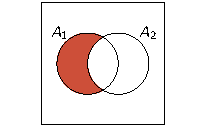
\includegraphics{Resources/Plots/Differenzmenge-1} \end{center}
\normalsize
\end{frame}

\begin{frame}{Grundlegende Begriffe}
\phantomsection\label{grundlegende-begriffe-16}
\framesubtitle{Ereignisse - QuizAcademy}

\QuizAcademy{Würfelwurf 1}\endQuizAcademy
\end{frame}

\begin{frame}[fragile]{Grundlegende Begriffe}
\phantomsection\label{grundlegende-begriffe-17}
\framesubtitle{Mengen in R}

\scriptsize

\begin{Shaded}
\begin{Highlighting}[]
\NormalTok{x }\OtherTok{\textless{}{-}} \FunctionTok{c}\NormalTok{(}\DecValTok{1}\NormalTok{,}\DecValTok{3}\NormalTok{,}\DecValTok{5}\NormalTok{)}
\NormalTok{y }\OtherTok{\textless{}{-}} \FunctionTok{c}\NormalTok{(}\DecValTok{2}\NormalTok{,}\DecValTok{3}\NormalTok{,}\DecValTok{6}\NormalTok{)}

\FunctionTok{union}\NormalTok{(x,y)}
\end{Highlighting}
\end{Shaded}

\begin{verbatim}
## [1] 1 3 5 2 6
\end{verbatim}

\begin{Shaded}
\begin{Highlighting}[]
\FunctionTok{intersect}\NormalTok{(x,y)}
\end{Highlighting}
\end{Shaded}

\begin{verbatim}
## [1] 3
\end{verbatim}

\begin{Shaded}
\begin{Highlighting}[]
\FunctionTok{setdiff}\NormalTok{(x,y)}
\end{Highlighting}
\end{Shaded}

\begin{verbatim}
## [1] 1 5
\end{verbatim}

\begin{Shaded}
\begin{Highlighting}[]
\FunctionTok{setdiff}\NormalTok{(y,x)}
\end{Highlighting}
\end{Shaded}

\begin{verbatim}
## [1] 2 6
\end{verbatim}

\begin{Shaded}
\begin{Highlighting}[]
\FunctionTok{setdiff}\NormalTok{(}\FunctionTok{union}\NormalTok{(x,y),y) }\CommentTok{\# Komplement von y, wenn Omega = union(x,y)}
\end{Highlighting}
\end{Shaded}

\begin{verbatim}
## [1] 1 5
\end{verbatim}

\normalsize
\end{frame}

\begin{frame}[fragile]{Grundlegende Begriffe}
\phantomsection\label{grundlegende-begriffe-18}
\framesubtitle{Mengen in R}

\tiny

\footnotesize

\begin{Shaded}
\begin{Highlighting}[]
\NormalTok{rje}\SpecialCharTok{::}\FunctionTok{powerSet}\NormalTok{(x)}
\end{Highlighting}
\end{Shaded}

\begin{verbatim}
## [[1]]
## numeric(0)
## 
## [[2]]
## [1] 1
## 
## [[3]]
## [1] 3
## 
## [[4]]
## [1] 1 3
## 
## [[5]]
## [1] 5
## 
## [[6]]
## [1] 1 5
## 
## [[7]]
## [1] 3 5
## 
## [[8]]
## [1] 1 3 5
\end{verbatim}

\normalsize

\normalsize
\end{frame}

\begin{frame}{Grundlegende Begriffe}
\phantomsection\label{grundlegende-begriffe-19}
\framesubtitle{Ereignisse}

\exe[]Ein Würfel wird einmal gewürfelt. Es sind folgende Ereignisse
definiert: \begin{gather*}
A_1=\{1,2\},\; A_2=\{3,4\},\; A_3=\{2,4\},\; A_4=\{1,2,3,4\},\\ A_5=\{4\}, A_6=\{3,4,5,6\}, A_7=\{5,6\},\; A_8=\{1,2,4,5\},\\ A_9=\{2,3,6\},\; A_{10}=\{1,4,5\}.
\end{gather*}

Bestimmen Sie folgende Ereignisse und stellen Sie diese jeweils in einem
Venn-Diagramm grafisch dar!

\begin{center}
\begin{tabular}{lll}
\blue{(a)} $A_1\cup A_2$ & \blue{(b)} $A_2\cap A_3$ & \blue{(c)} $\bar{A}_1$\\
\blue{(d)} $A_1\cap A_2$ & \blue{(e)} $A_8\cap\bar{A}_9=A_8\setminus A_9$ & \blue{(f)} $A_5\subset A_4$
\end{tabular}
\end{center}

\endexe
\end{frame}

\begin{frame}{Grundlegende Begriffe}
\phantomsection\label{grundlegende-begriffe-20}
\framesubtitle{Ereignisse}

\begin{itemize}
\tightlist
\item
  Jedes zusammengesetzte Ereignis \(A\) kann in disjunkte Teilereignisse
  \(A_j\neq\emptyset\) so zerlegt werden, dass gilt:
  \(A=\bigcup^n_{j=1} A_j\). \(A\) ergibt sich jetzt als disjunkte
  Vereinigung.
\item
  In Beispiel \ref{xmpl:potenz} lässt sich \(A_8\) in \(A_2=\{1\}\) und
  \(A_7=\{2,3\}\), aber auch in \(A_2=\{1\}\), \(A_3=\{2\}\) und
  \(A_4=\{3\}\) zerlegen. Beim zweiten Fall wurde \(A_8\) in
  Elementarereignisse zerlegt.
\item
  Die Zerlegung von \(A\) in Elementarereignisse heißt
  \hil{kanonische Darstellung}: Jedes Ereignis ergibt sich eindeutig als
  Vereinigungsereignis von Elementarereignissen:
\end{itemize}

\[A=\bigcup^n_{j=1}\{\omega_j\}.\]
\end{frame}

\begin{frame}{Grundlegende Begriffe}
\phantomsection\label{grundlegende-begriffe-21}
\framesubtitle{Vollständiges Ereignissystem}

\(\quad\)

\begin{itemize}
\tightlist
\item
  Da auch \(\Omega\) zu den zusammengesetzten Ereignissen gehört, kann
  es auch in (Teil-)Ereignisse \(A_j\) zerlegt werden.
\item
  Die Menge \(\{A_1,\ldots,A_n\}\) bildet ein \hil{vollständiges
  System von Ereignissen}, wenn für diese Zerlegung gilt:
\end{itemize}

\begin{align*}
(1) \qquad & \Omega=A_1\cup\ldots\cup A_n=\bigcup^n_{j=1}A_j,\\
(2) \qquad & A_i\cap A_j=\emptyset\quad\text{für  $i\neq j$},\\
(3) \qquad & A_j\neq\emptyset\quad\text{für $j=1,\ldots,n$},
\end{align*}

\begin{itemize}
\tightlist
\item
  Ein vollständiges System wird auch \hil{vollständiges Ereignissystem}
  bzw. \hil{vollständige Zerlegung} genannt.
\end{itemize}
\end{frame}

\begin{frame}{Grundlegende Begriffe}
\phantomsection\label{grundlegende-begriffe-22}
\framesubtitle{Vollständiges Ereignissystem}

\footnotesize
\begin{center}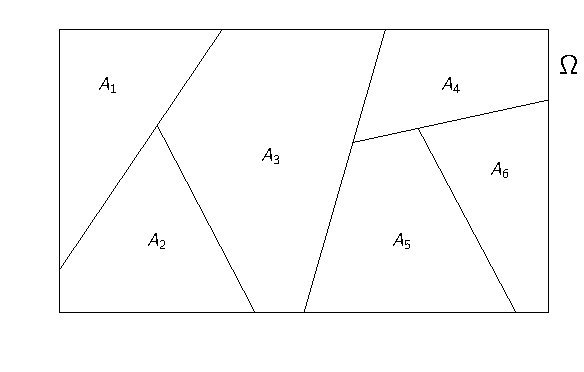
\includegraphics{Resources/Plots/unnamed-chunk-3-1} \end{center}
\normalsize
\end{frame}

\begin{frame}{Grundlegende Begriffe}
\phantomsection\label{grundlegende-begriffe-23}
\framesubtitle{Vollständiges Ereignissystem}
\vspace{1cm}

\exe

Ein Würfel wird einmal gewürfelt. Es sind folgende Ereignisse definiert:
\begin{gather*}
A_1=\{2,4,6\},\; A_2=\{1,3,5\},\; A_3=\{2\},\\
A_4=\{4,6\},\;A_5=\{1,3\}, A_6=\{5,6\}.
\end{gather*} Welche der folgenden Mengen bildet ein vollständiges
Ereignissystem?

\begin{enumerate}
[(a)]
\tightlist
\item
  \(F_1=\{A_1, A_2\}\)
\item
  \(F_2=\{A_1, A_5, A_6\}\)
\item
  \(F_3=\{A_3, A_4, A_5\}\)
\item
  \(F_4=\{A_2, A_3, A_4\}\)
\end{enumerate}

\endexe
\end{frame}

\begin{frame}{Der Wahrscheinlichkeitsbegriff}
\phantomsection\label{der-wahrscheinlichkeitsbegriff}
\begin{itemize}
\tightlist
\item
  Zufallsvorgänge zeichnen sich dadurch aus, dass ungewiss ist, welches
  ihrer möglichen Ereignisse eintritt.
\item
  Wahrscheinlichkeiten quantifizieren die Chance des Eintretens eines
  bestimmten Ereignisses und werden mit \(P\) symbolisiert.
\item
  Für ein Ereignis \(A\subset\Omega\) gibt \(P(A)\) jetzt die
  \hil{Wahrscheinlichkeit} für das Eintreten von \(A\) an.
\item
  \(P\) ist also eine Funktion, die Ereignissen reelle Zahlen zuordnet,
  welche wir als Wahrscheinlichkeit bezeichnen.
\end{itemize}
\end{frame}

\begin{frame}{Der Wahrscheinlichkeitsbegriff}
\phantomsection\label{der-wahrscheinlichkeitsbegriff-1}
\framesubtitle{Wahrscheinlichkeitfunktion und Kolmogoroff-Axiome}

\begin{itemize}
\tightlist
\item
  Die axiomatische Grundlage für Wahrscheinlichkeiten wurde von
  \hil{Kolmogoroff} entwickelt.
\item
  Auf der Basis dieser Axiomatik lässt sich die
  Wahrscheinlichkeitsfunktion wie folgt definieren:
\end{itemize}

\block{Kolmogoroff-Axiome}
\begin{itemize}\tightlist
\leftskip=12pt
\item[(K1)] $P(A)\geq 0$ für alle $A$,
\item[(K2)] $P(\Omega)=1$,
\item[(K3)] \[P\left(\bigcup^\infty_{j=1} A_j\right) = P(A_1)+P(A_2)  +\ldots=\sum^\infty_{j=1} P(A_j)\] für alle $A_i$ und $A_j$, die paarweise disjunkt sind: $A_i\cap A_j=\emptyset,$ $i\neq j$.
\end{itemize}

\endblock
\end{frame}

\begin{frame}{Der Wahrscheinlichkeitsbegriff}
\phantomsection\label{der-wahrscheinlichkeitsbegriff-2}
\framesubtitle{Wahrscheinlichkeitfunktion und Kolmogoroff-Axiome}

\block{Kolmogoroff-Axiome}
\begin{itemize}\tightlist
\leftskip=8pt
\item[(K1)] \hil{Nichtnegativität}: Die Wahrscheinlichkeit $P$ eines Ereignisses $A$ ist stets nichtnegativ.
\item[(K2)] \hil{Normierung} der Wahrscheinlichkeit.
\item[(K3)] \hil{Volladdidivität}: Die Wahrscheinlichkeit für die Vereinigung paarweise disjunkter Ereignisse gleicht der Summe der Einzelwahrscheinlichkeiten.
\end{itemize}
\endblock

Jedes Ereignis \(A\subset\Omega\) wird somit durch \(P\) in das
geschlossene Intervall \([0,1]\subset\mathbb{R}\) abgebildet.
\end{frame}

\begin{frame}{Der Wahrscheinlichkeitsbegriff}
\phantomsection\label{der-wahrscheinlichkeitsbegriff-3}
\framesubtitle{Rechenregeln}

Aus diesen Axiomen lassen sich folgende Rechenregeln ableiten:

\block{Rechenregeln}
 \begin{itemize}\tightlist\leftskip=12pt
\item[(R1)] $P(A)+P(\bar{A})=1,$
\item[(R2)] $P(A)\leq P(B)$ für $A\subset B$,
\item[(R3)] $P(A_1\cup A_2\cup\ldots\cup A_n)=\sum^n_{j=1}\limits P(A_j)$ (für paarweise disjunkte Ereignisse),
\item[(R4)] $P(A\cup B)=P(A)+P(B)-P(A\cap B)$ (für paarweise nicht disjunkte Ereignisse).
 \end{itemize}
\endblock

Ihre Herleitung findet sich im Buch auf S.~23.
\end{frame}

\begin{frame}{Der Wahrscheinlichkeitsbegriff}
\phantomsection\label{der-wahrscheinlichkeitsbegriff-4}
\framesubtitle{Rechenregeln - Additionssatz}

\[P(A\cup B)=P(A)+P(B)-\textcolor[RGB]{205,79,57}{P(A\cap B)}\]

\footnotesize
\begin{center}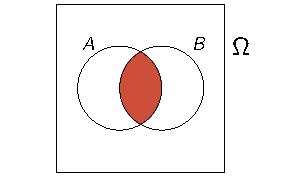
\includegraphics{Resources/Plots/unnamed-chunk-4-1} \end{center}
\normalsize

\begin{itemize}
\tightlist
\item
  \(A\) und \(B\) sind nicht disjunkt, da \(A\cap B \not=\emptyset\).
  \(A\cap B\) entspricht der roten Fläche.
\item
  \((A\cup B)\) würde mit \(P(A)+P(B)\) die Wahrscheinlichkeit für
  \(A\cap B\) doppelt erfassen; folglich muss \(P(A\cap B)\) subtrahiert
  werden.
\end{itemize}
\end{frame}

\begin{frame}{Der Wahrscheinlichkeitsbegriff}
\phantomsection\label{der-wahrscheinlichkeitsbegriff-5}
\framesubtitle{Rechenregeln}

\begin{itemize}
\tightlist
\item
  Der \hil{Additionssatz für disjunkte Ereignisse}
  \[P(A_1\cup A_2\cup\ldots\cup A_n)=\sum^n_{j=1}\limits P(A_j)\]
  liefert eine Vorschrift für die Wahrscheinlichkeit eines Ereignisses
  \(A=\{\omega_1,\omega_2,\ldots,\omega_n\}\) eines abzählbar
  unendlichen Stichprobenraumes \(\Omega\).
\item
  \hil{Elementarereignisse} \(\{\omega_j\},\) \(j=1,\ldots,n,\) sind
  paarweise disjunkt.
\end{itemize}
\end{frame}

\begin{frame}{Der Wahrscheinlichkeitsbegriff}
\phantomsection\label{der-wahrscheinlichkeitsbegriff-6}
\framesubtitle{Rechenregeln}

\exe[]Es sind folgende Wahrscheinlichkeiten gegeben:
\[P(A)=0.4, P(B)=0.7, P(A\cap B)=0.25.\] Bestimmen Sie die
Wahrscheinlichkeiten
\[P(A\cup B),\;P(\bar{B}),\;P(A\cap \bar{B}),\;P(A\cup \bar{B})\]
\endexe Wir verwenden einen Punkt anstelle eines Kommas als
\hil{Dezimaltrennzeichen}, da dies der angloamerikanischen Schreibweise
der Programmiersprache \R entspricht.
\end{frame}

\begin{frame}{Der Wahrscheinlichkeitsbegriff}
\phantomsection\label{der-wahrscheinlichkeitsbegriff-7}
\framesubtitle{Rechenregeln}
\exe

Ein Würfel wird ein Mal gewürfelt. Wie groß ist die Wahrscheinlichkeit,

\begin{enumerate}
[a)]
\tightlist
\item
  eine 2 oder eine 3 zu würfeln?
\item
  eine 2, eine 3 oder eine 4 zu würfeln?
\item
  eine ungerade Zahl oder eine gerade Zahl zu würfeln?
\item
  eine Augenzahl kleiner als 4 oder eine gerade Augenzahl zu würfeln?
\item
  eine Augenzahl kleiner als 4 und eine gerade Augenzahl zu würfeln?
\end{enumerate}

\endexe
\end{frame}

\begin{frame}{Der Wahrscheinlichkeitsbegriff}
\phantomsection\label{der-wahrscheinlichkeitsbegriff-8}
\framesubtitle{Rechenregeln}
\exe

In einer Urne befinden sich 20 rote und 30 grüne Kugeln. 5 rote und 10
grüne Kugeln sind mit einer 1 beschriftet. Wie groß ist die
Wahrscheinlichkeit, dass

\begin{enumerate}
[a)]
\tightlist
\item
  eine gezogene Kugel rot oder mit einer 1 beschriftet ist?
\item
  eine gezogene Kugel nicht mit einer 1 beschriftet ist?
\item
  eine rote Kugel gezogen wird und diese nicht mit einer 1 beschriftet
  ist?
\item
  eine Kugel gezogen wird, die rot oder nicht mit einer 1 beschriftet
  ist?
\end{enumerate}

\endexe
\end{frame}

\begin{frame}{Der Wahrscheinlichkeitsbegriff}
\phantomsection\label{der-wahrscheinlichkeitsbegriff-9}
\framesubtitle{Wahrscheinlichkeitsinterpretation}

\begin{itemize}
\tightlist
\item
  Mit den \hil{Axiomen von Kolmogoroff} und den Regeln \blue{(R1)} bis
  \blue{(R4)} sind nur die allgemeinen Eigenschaften der
  Wahrscheinlichkeiten festgelegt, nicht jedoch welche Werte sie bei
  bestimmten Ereignissen annehmen.
\item
  Hierzu muss eine dem Zufallsvorgang adäquate
  \hil{Wahrscheinlichkeitsinterpretation} vorliegen.
\end{itemize}

Mit dem subjektiven und statistisch/frequentistischen
Wahrscheinlichkeitsbegriff befasst sich das Buch auf S.~25.
\end{frame}

\begin{frame}{Der Wahrscheinlichkeitsbegriff}
\phantomsection\label{der-wahrscheinlichkeitsbegriff-10}
\framesubtitle{Objektive Wahrscheinlichkeit}

\begin{center}
\begin{tikzpicture}
\node[box] (a) {Objektive\\Wahrscheinlichkeitsinterpretation};
\node[box ,below of=a, xshift=-2cm, yshift=-1cm] (b) {a priori};
\node[box, below of=a, xshift=2cm, yshift=-0.5cm] (c) {statistisch\\frequentistisch};
\node[box, below of=b, xshift=-1.5cm, yshift=-0.25cm] (d) {klassisch\\(Laplace)};
\node[box, below of=b, xshift=1.5cm] (e) {geometrisch};
\draw[arrow] (a) to (b);
\draw[arrow] (a) to (c);
\draw[arrow] (b) to (d);
\draw[arrow] (b) to (e);
\end{tikzpicture}
\end{center}
\end{frame}

\begin{frame}{Der Wahrscheinlichkeitsbegriff}
\phantomsection\label{der-wahrscheinlichkeitsbegriff-11}
\framesubtitle{Objektive Wahrscheinlichkeit}

\exe

Student Paul kommt jeden Morgen zwischen 8.00 und 8.30 Uhr an einer
Bushaltestelle an, an der zwei Buslinien halten: \begin{gather*}
\text{Linie A:}\quad 8.04, 8.14, 8.24 \\ 
\text{Linie B:}\quad 8.10, 8.20, 8.30.
\end{gather*} Wie groß ist die Wahrscheinlichkeit, dass er Linie A
nimmt? \endexe
\end{frame}

\begin{frame}{Der Wahrscheinlichkeitsbegriff}
\phantomsection\label{der-wahrscheinlichkeitsbegriff-12}
\framesubtitle{Objektive Wahrscheinlichkeit}

\begin{itemize}
\tightlist
\item
  \hil{a-priori}:

  \begin{itemize}
  \item
    \hil{Laplace- (bzw. klassische) Wahrscheinlichkeit}: Anwendung bei
    Zufallsvorgängen mit endlichem \(\Omega\) und deren
    Elementarereignisse die gleiche Eintrittswahrscheinlichkeit besitzen
    (\hil{Laplace-Experimente}).
  \item
    Laplace-Experimente können als die zufällige Entnahme aus einer
    endlichen Menge von Objekten charakterisiert werden. Wird mehrfach
    gezogen, muss zwischen \emph{Ziehen mit Zurücklegen} oder
    \emph{Ziehen ohne Zurücklegen} unterschieden werden.
  \end{itemize}
\end{itemize}
\end{frame}

\begin{frame}{Der Wahrscheinlichkeitsbegriff}
\phantomsection\label{der-wahrscheinlichkeitsbegriff-13}
\framesubtitle{Laplace-Wahrscheinlichkeit}

\block{Laplace-Wahrscheinlichkeit}

Die Wahrscheinlichkeit für ein Elementarereignis \(\{\omega_i\},\)
\(i=1,\ldots,m\) beträgt dann \(P(\{\omega_i\})=\frac{1}{m}\).\mps

\(P(A)\) erhält man als \[
  P(A)=\dfrac{\text{Anzahl der für $A$ günstigen Ausgänge}}{\text{Anzahl der möglichen Ausgänge}}.
  \] Die Anzahl der Elemente einer Menge \(M\) heißt \hil{Mächtigkeit}
\(|M|\). Die Laplace-Wahrscheinlichkeit ist dann
\[P(A)=\frac{|A|}{|\Omega|}.\] \endblock
\end{frame}

\begin{frame}{Der Wahrscheinlichkeitsbegriff}
\phantomsection\label{der-wahrscheinlichkeitsbegriff-14}
\framesubtitle{Laplace-Wahrscheinlichkeit - QuizAcademy}

\QuizAcademy{Würfelwurf 2}\endQuizAcademy
\end{frame}

\begin{frame}{Der Wahrscheinlichkeitsbegriff}
\phantomsection\label{der-wahrscheinlichkeitsbegriff-15}
\framesubtitle{Laplace-Wahrscheinlichkeit}
\exe[Laplace-Experimente]

\begin{enumerate}
[(a)]
\tightlist
\item
  In einer Urne befinden sich 20 Kugeln, von denen 8 rot sind. Berechnen
  Sie die Wahrscheinlichkeit eine rote Kugel bei einer zufälligen
  Entnahme zu erhalten.
\item
  Wie groß ist die Wahrscheinlichkeit, nach Ziehen einer roten Kugel
  ohne Zurücklegen im zweiten Zug erneut eine rote Kugel zu ziehen?
\item
  Ein \hil{Laplace-Würfel} (idealer Würfel) wird geworfen. Berechnen Sie
  die Wahrscheinlichkeit, dass eine Augenzahl größer als 2 oben liegt.
\end{enumerate}

\endexe
\end{frame}

\begin{frame}{Der Wahrscheinlichkeitsbegriff}
\phantomsection\label{der-wahrscheinlichkeitsbegriff-16}
\framesubtitle{Laplace-Wahrscheinlichkeit}

\exe[]Ein Laplace-Würfel wird einmal geworfen. Wie groß ist die
Wahrscheinlichkeit, dass eine Augenzahl kleiner 3 fällt? \endexe
\exe[]Eine Laplace-Münze und ein Laplace-Würfel werden gemeinsam
geworfen. Wie groß ist die Wahrscheinlichkeit, dass Kopf und eine
Augenzahl größer als 4 fällt? \endexe
\end{frame}

\begin{frame}{Bedingte Wahrscheinlichkeit}
\phantomsection\label{bedingte-wahrscheinlichkeit}
\framesubtitle{Änderung des Stichprobenraums}
\vspace{1cm}

\begin{itemize}
\tightlist
\item
  Die Berechnung von Wahrscheinlichkeiten erfolgt bislang unter Bezug
  auf den ganzen Stichprobenraum \(\Omega\).
\item
  Es lassen sich aber auch dann Wahrscheinlichkeiten für \(A\)
  berechnen, wenn nicht ganz \(\Omega\), sondern nur noch ein Teil \(B\)
  davon relevant ist. Die Abbildung verdeutlicht die Veränderung des
  Bezugssystems.
\end{itemize}

\vspace{-.5cm}

\footnotesize
\begin{center}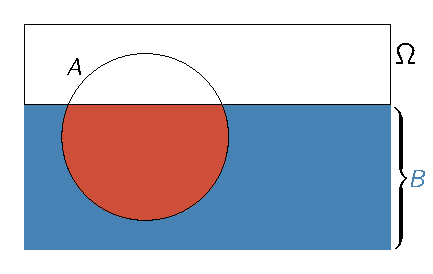
\includegraphics{Resources/Plots/BedingteWkeit-1} \end{center}
\normalsize
\end{frame}

\begin{frame}{Bedingte Wahrscheinlichkeit}
\phantomsection\label{bedingte-wahrscheinlichkeit-1}
\framesubtitle{Änderung des Stichprobenraums}

\begin{itemize}
\tightlist
\item
  Der Kreis entspricht \(A\), das untere Rechteck \(B\) und das rote
  Kreissegment \(A\cap B\).
\item
  \(P(A)\), \(P(B)\) und \(P(A\cap B)\) sind die Wahrscheinlichkeiten
  für \(A\), \(B\) und \(A\cap B\), wenn \(\Omega\) zugrunde liegt.
\item
  Es kann aber auch die Wahrscheinlichkeit für \(A\) unter der Bedingung
  berechnet werden, dass nur noch die Ausgänge in \(B\) relevant sind.
\item
  Diese \hil{bedingte Wahrscheinlichkeit} wird mit \(P(A|B)\)
  bezeichnet.
\item
  In der Abbildung ist \(P(A)\) das Verhältnis der Kreisfläche zur
  Fläche des Rechtecks \(\Omega\); die bedingte Wahrscheinlichkeit
  \(P(A|B)\) jedoch das Verhältnis der roten Fläche zur Fläche des
  Rechtecks \(B\).
\end{itemize}
\end{frame}

\begin{frame}{Bedingte Wahrscheinlichkeit}
\phantomsection\label{bedingte-wahrscheinlichkeit-2}
\framesubtitle{Formel}

\begin{block}{Bedingte Wahrscheinlichkeit}
 Es seien $A$, $B\subset\Omega$ Ereignisse
 und %$(\Omega, A, P)$ der Wahrscheinlichkeitsraum,
 $P(B) > 0$. Für die \hil{bedingte Wahrscheinlichkeit} $P(A|B)$ gilt \[ P(A|B) = \frac{P(A\cap B)}{P(B)}. \]
\end{block}
\end{frame}

\begin{frame}{Bedingte Wahrscheinlichkeit}
\phantomsection\label{bedingte-wahrscheinlichkeit-3}
\framesubtitle{Beispiele}

\xmpl[Idealer Würfel]Ein idealer Würfel wird geworfen. Also sind
\(\Omega =\{1,2,\ldots,6\}\) und \(P(\{\omega_i\}) = 1/6\) für
\(i=1,\ldots,6\). \medskip

\(A\) ist das Ereignis, eine \emph{1} zu würfeln; \(B\) das Ereignis
einer ungeraden Augenzahl. \(A\cap B\) tritt bei einer \emph{1} ein. Die
Wahrscheinlichkeiten betragen \(P(A) = 1/6,\) \(P(B) = 1/2\) und
\(P(A\cap B) = 1/6\). \medskip

Was ist nun die Wahrscheinlichkeit einer \emph{1} unter der Bedingung,
dass eine ungerade Augenzahl eintritt? Der durch die Bedingung gegebene
Stichprobenraum lautet \(B = \{1,3,5\}\), also gilt \(P(A|B)=1/3.\)
\medskip

Denselben Wert erhält man nach der eingeführten Definition:
\[ P(A|B) = \frac{P(A\cap B)}{P(B)} = \frac{\frac{1}{6}}{\frac{1}{2}}=\frac{1}{3}.\]
\endxmpl
\end{frame}

\begin{frame}{Bedingte Wahrscheinlichkeit}
\phantomsection\label{bedingte-wahrscheinlichkeit-4}
\framesubtitle{Aufgaben}
\exe

Nach der achtmaligen Durchführung des Zufallsexperiments
\emph{zweimaliges Werfen einer Münze} erhält man folgendes Resultat:

\begin{center}
\begin{tabular}{l|cccccccc}
Versuch & 1 & 2 & 3 & 4 & 5 & 6 & 7 & 8\\ \hline
1. Wurf & K & Z & Z & Z & K & Z & Z & K\\
2. Wurf & Z & Z & K & K & K & Z & K & Z
\end{tabular}
\end{center}

Ereignis \(A\): K beim 1. Wurf,\quad Ereignis \(B\): K beim 2. Wurf

Berechnen Sie folgende Wahrscheinlichkeiten:

\begin{center}
\begin{tabular}{lll}
\blue{(a)} $P(A)$   & \blue{(b)} $P(B)$   & \blue{(c)} $P(A\cap B)$\\
\blue{(d)} $P(A|B)$ & \blue{(e)} $P(B|A)$ & \\
\end{tabular}
\end{center}
\endexe
\end{frame}

\begin{frame}{Bedingte Wahrscheinlichkeit}
\phantomsection\label{bedingte-wahrscheinlichkeit-5}
\framesubtitle{Aufgaben}
\exe

In einem Dorf leben 1000 Personen. Es ist bekannt, dass 600 Einwohner
nach Mallorca in den Urlaub fahren und dass 500 Einwohner die
Bild--Zeitung lesen. Zusätzlich weiß man, dass von den 600
Mallorca--Urlaubern 400 die Bild lesen. Wie groß ist die
Wahrscheinlichkeit, dass

\begin{enumerate}
[(a)]
\tightlist
\item
  eine Person Mallorca--Urlauber ist,
\item
  eine Person Bild--Zeitung--Leser ist,
\item
  eine Person Mallorca--Urlauber und Bild--Zeitung--Leser ist,
\item
  wenn ein Einwohner Bild--Zeitung liest, dieser auch ein
  Mallorca--Urlauber ist,
\item
  wenn ein Einwohner Mallorca--Urlauber ist, dieser auch Bild--Zeitung
  liest?
\end{enumerate}

\endexe
\end{frame}

\begin{frame}{Bedingte Wahrscheinlichkeit}
\phantomsection\label{bedingte-wahrscheinlichkeit-6}
\framesubtitle{Paarweise stochastische Unabhängigkeit}

\begin{itemize}
\tightlist
\item
  \(P(A|B)\) lässt sich als die Wahrscheinlichkeit von \(A\) unter der
  zusätzlichen Information interpretieren, dass \(B\) bereits
  eingetreten ist.
\item
  Übt diese Information keinen Einfluss auf die Wahrscheinlichkeit von
  \(A\) aus, gilt \(P(A|B)=P(A)\).
\item
  \(A\) ist dann \hil{unabhängig} von \(B\).
\item
  Dann ist aber auch \(B\) unabhängig von \(A\), wie folgende Umformung
  zeigt: \begin{align*}
  P(B|A) & = \frac{P(A\cap B)}{P(A)}=\frac{P(A|B)P(B)}{P(A)} \\
   & = \frac{P(A)P(B)}{P(A)}=P(B)\;\;\; (\text{wegen }P(A|B)=P(A)).
  \end{align*}
\end{itemize}
\end{frame}

\begin{frame}{Bedingte Wahrscheinlichkeit}
\phantomsection\label{bedingte-wahrscheinlichkeit-7}
\framesubtitle{Paarweise stochastische Unabhängigkeit - QuizAcademy}
\QuizAcademy{Würfelwurf 3}\endQuizAcademy
\end{frame}

\begin{frame}{Bedingte Wahrscheinlichkeit}
\phantomsection\label{bedingte-wahrscheinlichkeit-8}
\framesubtitle{Paarweise stochastische Unabhängigkeit}

\begin{itemize}
\tightlist
\item
  Diese über die Wahrscheinlichkeiten festgelegte Eigenschaft zweier
  Ereignisse heißt \hil{paarweise stochastische Unabhängigkeit}.
\item
  Dies liefert eine einfache Prüfung auf stochastische Unabhängigkeit:
  \defn[Paarweise stochastische Unabhängigkeit]Zwei Ereignisse \(A\) und
  \(B\) heißen \hil{paarweise stochastisch unabhängig}, wenn eine der
  drei folgenden Bedingungen erfüllt ist: \begin{eqnarray*}
   & & (1) \quad P(A\cap B)=P(A)P(B), \\
   & & (2) \quad P(A|B)=P(A) \quad\text{falls } P(B)>0, \\
   & & (3) \quad P(B|A)=P(B) \quad \text{falls } P(A)>0;
  \end{eqnarray*} andernfalls bezeichnet man sie als
  \hil{stochastisch abhängig}. \enddefn
\end{itemize}
\end{frame}

\begin{frame}{Bedingte Wahrscheinlichkeit}
\phantomsection\label{bedingte-wahrscheinlichkeit-9}
\framesubtitle{Paarweise stochastische Unabhängigkeit}

\xmpl[Zweimaliges Würfeln]Ein idealer Würfel wird zweimal geworfen.
\(A\) sei die \emph{Augenzahl 1 im ersten Wurf}; \(B\) sei die
\emph{Augenzahl 2 im zweiten Wurf}.

Der Stichprobenraum umfasst 36 geordnete Zahlenpaare, weil zu
unterscheiden ist, wann welche Augenzahl eintritt:
\[ \Omega = \{(1,1),\ldots,(1,6),\ldots,(6,1),\ldots,(6,6)\}. \]
\endxmpl
\end{frame}

\begin{frame}{Bedingte Wahrscheinlichkeit}
\phantomsection\label{bedingte-wahrscheinlichkeit-10}
\vspace{0.8cm}
\framesubtitle{Paarweise stochastische Unabhängigkeit}

\xmpl[*]Für die Ereignisse erhält man: \begin{alignat*}{2}
& A=\{(1,1),\ldots,(1,6)\}& , & \;
 P(A)=\frac{|A|}{|\Omega|}=\frac{6}{36}=\frac{1}{6},\\
& B=\{(1,2),\ldots,(6,2)\}& , & \;
P(B)=\frac{|B|}{|\Omega|}=\frac{6}{36}=\frac{1}{6}, \\
& A \cap B=\{(1,2)\}& , & \; P(A\cap B)=\frac{|A\cap B|}{|\Omega|}=\frac{1}{36}.
\end{alignat*} Wegen
\[P(A\cap B)=\frac{1}{36}=P(A)P(B)=\frac{1}{6}\cdot \frac{1}{6}\] folgt
paarweise stochastische Unabhängigkeit. \endxmpl
\end{frame}

\begin{frame}{Bedingte Wahrscheinlichkeit}
\phantomsection\label{bedingte-wahrscheinlichkeit-11}
\vspace{1cm}
\framesubtitle{Paarweise stochastische Unabhängigkeit}
\exe

Aus einer Urne mit vier Kugeln mit den Ziffern 1,2,3,4 wird eine
entnommen. Für welche Ereignisse liegt paarweise stochastische
Unabhängigkeit vor?

\begin{enumerate}
[(a)]
\tightlist
\item
  \(A=\{1,2\}\), \(B=\{1\}\)
\item
  \(A=\{1,2,3\}\), \(B=\{1,2,4\}\)
\item
  \(A=\{1,2\}\), \(B=\{1,3\}\)
\end{enumerate}

\endexe

\begin{itemize}
\item
  Das Buch auf S.\nbs 34 diskutiert die Verallgemeinerung der
  stochastischen Unabhängigkeit auf mehr als zwei Ereignisse.
\item
  Sind Ereignisse gemeinsam stochastisch unabhängig, dann sind sie auch
  paarweise stochastisch unabhängig. Die Umkehrung gilt allerdings
  nicht!
\end{itemize}
\end{frame}

\begin{frame}{Bedingte Wahrscheinlichkeit}
\phantomsection\label{bedingte-wahrscheinlichkeit-12}
\framesubtitle{Multiplikationssätze}

Mit dem Konzept der bedingten Wahrscheinlichkeiten lassen sich nützliche
Sätze der Wahrscheinlichkeitsalgebra gewinnen:

\defn[Multiplikationssatz für 2 Ereignisse]Es seien \(A,B\subset\Omega\)
Ereignisse mit \(P(A)>0\) und \(P(B)>0\). Dann gilt

\begin{enumerate}
[(a)]
\tightlist
\item
  bei stochastischer Abhängigkeit:
  \[ P(A\cap B)=P(A|B)P(B)=P(B|A)P(A);\]
\item
  bei stochastischer Unabhängigkeit: \[ P(A\cap B)=P(A)P(B).\]
\end{enumerate}

\enddefn
\end{frame}

\begin{frame}{Bedingte Wahrscheinlichkeit}
\phantomsection\label{bedingte-wahrscheinlichkeit-13}
\framesubtitle{Multiplikationssätze}

Die Verallgemeinerung der Ergebnisse des Multiplikationssatzes für zwei
Ereignisse führt zum Multiplikationssatz für \(n\) Ereignisse:
\defn[Multiplikationssatz für $n$ Ereignisse]Es seien
\(A_j\subset\Omega,\) \(j=1,\ldots,n\) Ereignisse mit
\(A_1\cap A_2\cap\ldots\cap A_{n-1}\neq\emptyset\). Dann gilt

\begin{enumerate}
[(a)]
\tightlist
\item
  bei stochastischer Abhängigkeit: \vspace{-0.5cm}
\end{enumerate}

\begin{align*}
P(A_1\cap A_2\cap\ldots\cap A_n) = & P(A_1)P(A_2|A_1)P(A_3|A_1\cap
A_2)\cdot\ldots \\\nonumber
& \cdot P(A_n|A_1\cap A_2\cap\ldots\cap A_{n-1});
\end{align*}

\begin{enumerate}
[(a)]
\setcounter{enumi}{1}
\tightlist
\item
  bei gemeinsamer stochastischer Unabhängigkeit:
  \begin{equation}\label{gemWSUnabh}
  P(A_1\cap A_2\cap\ldots\cap A_n) = P(A_1)P(A_2)\cdot\ldots\cdot P(A_n).
  \end{equation}
\end{enumerate}

\enddefn
\end{frame}

\begin{frame}{Bedingte Wahrscheinlichkeit}
\phantomsection\label{bedingte-wahrscheinlichkeit-14}
\framesubtitle{Multiplikationssätze}

\xmpl[Geburten]Ein Ehepaar möchte wissen welche der drei folgenden
Anordnungen von vier Kindern am wahrscheinlichsten ist: JJJJ, MMMM oder
JMJM.\newline \newline Wir unterstellen, dass die Wahrscheinlichkeiten
für einen \emph{Jungen} (J) und ein \emph{Mädchen} (M) jeweils 0.5 sind.
Dann sind alle drei Anordnungsmöglichkeiten gleich
wahrscheinlich.\newline \newline Der Grund dafür ist, dass die
Ereignisse gemeinsam stochastisch unabhängig sind:
\[P(\text{JJJJ})=P(\text{MMMM})=P(\text{JMJM})=0.5\cdot 0.5\cdot 0.5\cdot 0.5=0.5^4=0.0625.\]
Die Wahrscheinlichkeit für 2 J und 2 M ist allerdings wesentlich höher:
\[P(\text{2J und 2M})=\dfrac{6}{16}=0.375.\] \endxmpl
\end{frame}

\begin{frame}{Bedingte Wahrscheinlichkeit}
\phantomsection\label{bedingte-wahrscheinlichkeit-15}
\framesubtitle{Multiplikationssätze}
\exe

Eine Urne enthält 5 weiße und 5 rote Kugeln. Wie groß ist die
Wahrscheinlichkeit, dass gleich die ersten drei Kugeln, die gezogen
werden, rot sind (ZoZ)? \endexe

\exe

In einer Urne befinden sich 3 schwarze und 2 weiße Kugeln. Wie groß ist
die Wahrscheinlichkeit, nach dreimaligem Ziehen ohne Zurücklegen

\begin{enumerate}
[(a)]
\tightlist
\item
  eine weiße Kugel im zweiten Zug,
\item
  im dritten Zug die erste weiße Kugel,
\item
  alle weißen Kugeln
\end{enumerate}

zu ziehen? \endexe
\end{frame}

\begin{frame}{Bedingte Wahrscheinlichkeit}
\phantomsection\label{bedingte-wahrscheinlichkeit-16}
\framesubtitle{Satz von der totalen Wahrscheinlichkeit}

Jede Wahrscheinlichkeit \(P(B)>0\) kann auf bedingte
Wahrscheinlichkeiten zurückgeführt werden: \medskip
\defn[Satz von der totalen Wahrscheinlichkeit]\label{SatztotWS} Es sei
\(\{A_1,\ldots,A_n\},\) mit \(A_j\) für \(j=1,\ldots,n\) ein
vollständiges System von Ereignissen. Für das Ereignis \(B\) gilt dann
\begin{align}
P(B) & =P(B|A_1)P(A_1)+P(B|A_2)P(A_2)+\ldots+P(B|A_n)P(A_n)\notag\\
 & = \sum^n_{j=1}\limits P(B|A_j)P(A_j).
\end{align} \enddefn
\end{frame}

\begin{frame}{Bedingte Wahrscheinlichkeit}
\phantomsection\label{bedingte-wahrscheinlichkeit-17}
\vspace{.5cm}
\framesubtitle{Satz von der totalen Wahrscheinlichkeit}
\setlength{\medskipamount}{=6pt plus 0pt minus 6pt}

\begin{itemize}
\tightlist
\item
  Die folgende Abbildung zeigt eine solche Zerlegung:
\end{itemize}

\vspace{-.5cm}

\footnotesize
\begin{center}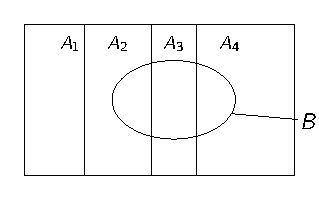
\includegraphics{Resources/Plots/Zerlegung-1} \end{center}
\normalsize

\begin{itemize}
\tightlist
\item
  \(P(B)\) ist gleich dem gewogenen arithmetischen Mittel der bedingten
  Wahrscheinlichkeiten \(P(B|A_j)\) mit Gewichten \(P(A_j)\):
  \[ P(B)=\sum^n_{j=1}P(B|A_j)P(A_j).\]
\end{itemize}
\end{frame}

\begin{frame}{Bedingte Wahrscheinlichkeit}
\phantomsection\label{bedingte-wahrscheinlichkeit-18}
\framesubtitle{Satz von der totalen Wahrscheinlichkeit}
\exe

In Urne 1 befinden sich 14 weiße und 6 schwarze Kugeln, in Urne 2
befinden sich 2 weiße und 8 schwarze Kugeln und in Urne 3 befinden sich
3 weiße und 7 schwarze Kugeln.

Um aus einer Urne Kugeln entnehmen zu dürfen, muss man würfeln. Bei
einer 1, 2 oder 3 darf man eine Kugel aus Urne 1 ziehen, bei einer 4
oder 5 aus Urne 2 und bei einer 6 aus Urne 3.

Wie groß ist die Wahrscheinlichkeit eine weiße Kugel zu ziehen? \endexe

\exe

In einer Stadt sind 60\% der Einwohner Frauen und 40\% Männer. Es ist
bekannt, dass 30\% der Frauen und 50\% der Männer rauchen.

Wie groß ist die Wahrscheinlichkeit, dass ein Raucher männlich ist?
\endexe
\end{frame}

\begin{frame}{Bedingte Wahrscheinlichkeit}
\phantomsection\label{bedingte-wahrscheinlichkeit-19}
\framesubtitle{Bayes'sches Theorem}

\begin{itemize}
\tightlist
\item
  Mit dem \hil{Satz für die bedingte Wahrscheinlichkeit} und dem
  \hil{Multiplikationssatz für 2 Ereignisse} lässt sich eine weitere
  Regel gewinnen, vorausgesetzt \(P(B)>0\): \begin{align*}
   P(A_i|B)& = \frac{P(A_i\cap B)}{P(B)}\quad \text{(nach Satz für bedingte Wahrscheinlichkeit)} \\
   & = \frac{P(B|A_i)P(A_i)}{P(B)} \quad \text{(nach Multiplikationssatz)}
   \end{align*}
\item
  Ersetzt man im letzten Bruch \(P(B)\) durch den Satz der totalen
  Wahrscheinlichkeit \eqref{SatztotWS}, erhält man das
  \hil{Bayes'sche Theorem}:
\end{itemize}

\defn[Satz von Bayes]
 \[ P(A_i|B)=\frac{P(B|A_i)P(A_i)}{\sum^n_{j=1}P(B|A_j)P(A_j)} \; \text{
 für alle } i=1, \ldots, n. \] \enddefn
\end{frame}

\begin{frame}{Bedingte Wahrscheinlichkeit}
\phantomsection\label{bedingte-wahrscheinlichkeit-20}
\framesubtitle{Bayes'sches Theorem}

\begin{itemize}
\tightlist
\item
  Das Theorem von Bayes gibt an, wie die Wahrscheinlichkeit für ein
  Ereignis \(A\) nach Durchführen eines Experimentes oder einer
  Beobachtung neu berechnet werden kann.
\item
  Interpretiere hierzu das vollständige Ereignissystem \(A_j\),
  \(j=1,\ldots,n\) als Menge sich ausschließender Hypothesen oder
  disjunkter Zustände. Die Wahrscheinlichkeiten \(P(A_j)\) sind aufgrund
  von Ausgangsinformationen bestimmt; sie sind daher
  \hil{a-priori-Wahrscheinlichkeiten} für jedes \(A_j\).
\item
  Mit dem Bayes'schen Theorem erhält man jetzt die
  \hil{a-posteriori-Wahrscheinlichkeiten} für \(A_j\), wenn die
  Beobachtung \(B\) bzw. das experimentelle Ergebnis \(B\) vorliegt. Das
  Eintreten des Ereignisses \(B\) ist eine zusätzliche Information.
\end{itemize}
\end{frame}

\begin{frame}{Bedingte Wahrscheinlichkeit}
\phantomsection\label{bedingte-wahrscheinlichkeit-21}
\framesubtitle{Bayes'sches Theorem}

\xmpl[Bayes'sches Theorem]Ein Test erkennt eine Krankheit mit einer
Wahrscheinlichkeit von 95\%, wenn diese tatsächlich vorliegt. Es gibt
aber auch \emph{falsche positive} Befunde mit einer Wahrscheinlichkeit
von 1\%. 0.1\% der Bevölkerung hat die Krankheit. Was ist die
Wahrscheinlichkeit, dass eine Person die Krankheit hat, wenn der Test
positiv ausfällt? \begin{eqnarray*}
P(K|+)=\frac{P\left(+|K\right) P(K)}{P(+)}=\frac{0.95\cdot0.001}{0.95\cdot0.001+0.01\cdot 0.999}=0.0868,
\end{eqnarray*} wobei \(\Omega=K\cup \bar{K}\) mit
\(K\cap \bar{K}=\emptyset\) und daher: \begin{eqnarray*}
P(+)&=&P(+\cap K)+P(+\cap \bar{K})\\
&=&P\left(+|K\right) P(K)+P\left(+|\bar{K}\right) P(\bar{K}).
\end{eqnarray*} \endxmpl
\end{frame}

\begin{frame}{Bedingte Wahrscheinlichkeit}
\phantomsection\label{bedingte-wahrscheinlichkeit-22}
\framesubtitle{Bayes'sches Theorem}

\xmpl[*]Der Satz von Bayes findet in sehr vielen unterschiedlichen
Disziplinen Anwendung, z.B. wie
\href{https://www.spiegel.de/politik/deutschland/kommentar-die-ermittlungen-im-fall-edathy-muessen-weitergehen-a-953963.html}{hier}
zu sehen auch in der Justiz. \medskip

Oder auch in Situationen des alltäglichen Lebens wie
\href{http://www.businessinsider.com/dating-for-bayesians-heres-how-to-use-statistics-to-improve-your-love-life-2013-11}{hier}.
\medskip

Auch Spamfilter funktionieren nach diesem Prinzip. \endxmpl
\end{frame}

\begin{frame}{Bedingte Wahrscheinlichkeit}
\phantomsection\label{bedingte-wahrscheinlichkeit-23}
\framesubtitle{Bayes'sches Theorem}
\exe

Das Angelrevier eines Hobbyanglers besteht aus den drei Seen S1, S2 und
S3, wobei er keinen der drei Seen bevorzugt. \medskip

Die Wahrscheinlichkeit dafür, dass er innerhalb einer Stunde einen Fisch
fängt, beträgt für den See S1 60\%, für den See S2 50\% und für den See
S3 80\%. \medskip

Nach einer Stunde Angelzeit kann sich der Hobbyangler über den Fang
eines Fisches freuen. Wie groß ist die Wahrscheinlichkeit, dass der
Fisch in dem See S2 geangelt wurde? \endexe
\end{frame}

\begin{frame}{Bedingte Wahrscheinlichkeit}
\phantomsection\label{bedingte-wahrscheinlichkeit-24}
\framesubtitle{Bayes'sches Theorem}
\exe

Ein Autohersteller bezieht Airbags von 2 Zulieferern. Beim Zulieferer 1,
der insgesamt 65\% aller Airbags liefert, sind 98\% der Airbags
fehlerfrei. 95\% der von Zulieferer 2 gelieferten Airbags sind nicht
defekt.

\begin{enumerate}
[(a)]
\tightlist
\item
  Wenn der Hersteller ein fehlerhaftes Teil bekommt, wie groß ist die
  Wahrscheinlichkeit, dass es von Zulieferer 1 kommt?
\item
  Wie groß ist die Wahrscheinlichkeit, dass ein fehlerhaftes Airbag von
  Zulieferer 2 kommt?
\item
  Wie groß ist die Wahrscheinlichkeit, dass ein geliefertes Airbag
  defekt ist?
\end{enumerate}

\endexe
\end{frame}

\begin{frame}{Kombinatorik}
\phantomsection\label{kombinatorik}
\framesubtitle{Grundlagen}

\begin{itemize}
\tightlist
\item
  Zur Berechnung von Wahrscheinlichkeiten nach dem klassischen Konzept
  müssen die \glqq{}günstigen\grqq{} Ausgänge zu den möglichen Ausgängen
  ins Verhältnis gesetzt werden.
\item
  Oft ist aber gerade die Ermittlung der günstigen Ausgänge nicht
  einfach.
\item
  Formeln für ihre Berechnung sind daher nützlich. Der Zweig der
  Mathematik, der sich hiermit beschäftigt, ist die \hil{Kombinatorik}.
\item
  Sie untersucht die verschiedenen Möglichkeiten der Anordnung oder
  Auswahl von Objekten, im Folgenden \glqq{}Elemente\grqq{}.
\end{itemize}
\end{frame}

\begin{frame}{Kombinatorik}
\phantomsection\label{kombinatorik-1}
\framesubtitle{Permutation ohne Wiederholung}

\begin{itemize}
\tightlist
\item
  Die Entwicklung der Kombinatorikformeln lässt sich anschaulich an
  einer Gesamtheit mit \(N\) nummerierten Kugeln \(1,2,\ldots,N\)
  zeigen.
\item
  Jede Zusammenstellung aller \(N\) Kugeln (Zahlen) in irgendeiner
  Anordnung ist eine \hil{Permutation}. Die Anzahl unterscheidbarer
  Permutationen erhält man durch folgende Überlegung.
\end{itemize}
\end{frame}

\begin{frame}{Kombinatorik}
\phantomsection\label{kombinatorik-2}
\framesubtitle{Permutation ohne Wiederholung}

\begin{itemize}
\tightlist
\item
  Um die erste Stelle der Anordnung zu besetzen, stehen \(N\) Kugeln zur
  Auswahl. Danach bleiben zur Besetzung der zweiten Stelle \(N-1\), für
  die dritte Stelle \(N-2\) Kugeln und schließlich für die letzte
  (\(N\)-te) Stelle nur noch eine Kugel übrig.
\item
  Die Gesamtzahl unterscheidbarer Permutationen ist das Produkt aus all
  diesen Besetzungsmöglichkeiten, also
  \[ N(N-1)(N-2)\cdot\ldots\cdot 1.\]
\end{itemize}
\end{frame}

\begin{frame}{Kombinatorik}
\phantomsection\label{kombinatorik-3}
\framesubtitle{Permutation ohne Wiederholung}

\begin{itemize}
\tightlist
\item
  Ein solches Produkt heißt \hil{$N$--Fakultät}, geschrieben als \(N!\),
  wobei \(N\in\mathbb{N}\).
\item
  Für \(N=4\) erhält man \(4! = 4\cdot 3 \cdot 2 \cdot 1 = 24\), für
  \(N=1\): \(1! = 1\).
\item
  Damit die Rekursionsformel \(N!=N(N-1)!\) uneingeschränkt auf
  \(\mathbb{N}\) gilt, definiere zudem \(0!=1\).
\item
  Bezeichnet man die Permutationen mit \(P\), gibt der folgende Satz die
  Anzahl der Anordnungen von \(N\) verschiedenen Elementen wieder:
  \defn[Permutation ohne Wiederholung]
   \[ P(N)=N!=N(N-1)(N-2)\cdot\ldots\cdot 1.\] \enddefn
\end{itemize}
\end{frame}

\begin{frame}{Kombinatorik}
\phantomsection\label{kombinatorik-4}
\framesubtitle{Permutation ohne Wiederholung - QuizAcademy}

\QuizAcademy{Kombinatorik}\endQuizAcademy
\end{frame}

\begin{frame}{Kombinatorik}
\phantomsection\label{kombinatorik-5}
\framesubtitle{Permutation ohne Wiederholung}

\xmpl[Kugeln]Es sollen drei Kugeln mit den Ziffern 1, 2 und 3
unterschiedlich angeordnet werden. Die möglichen Permutationen lauten:
\begin{align*}
\begin{matrix}
1 &  2 & 3 \\
2 &  1 & 3
\end{matrix} \qquad\quad
\begin{matrix}
1 & 3 & 2 \\
2 & 3 & 1
\end{matrix} \qquad\quad
\begin{matrix}
3 & 1 & 2 \\
3 & 2 & 1
\end{matrix}
\end{align*} Ihre Anzahl erhält man nach der Formel für Permutationen
ohne Wiederholung als \center \(3! = 6\). \endxmpl
\end{frame}

\begin{frame}[fragile]{Kombinatorik}
\phantomsection\label{kombinatorik-6}
\framesubtitle{Permutationen ohne Wiederholung in \R}

\footnotesize

\begin{Shaded}
\begin{Highlighting}[]
\DocumentationTok{\#\#\# Beispiel: Kugeln (1/3)}
\FunctionTok{prod}\NormalTok{(}\DecValTok{1}\SpecialCharTok{:}\DecValTok{3}\NormalTok{)}
\end{Highlighting}
\end{Shaded}

\begin{verbatim}
## [1] 6
\end{verbatim}

\begin{Shaded}
\begin{Highlighting}[]
\FunctionTok{factorial}\NormalTok{(}\DecValTok{3}\NormalTok{) }\CommentTok{\# kürzer}
\end{Highlighting}
\end{Shaded}

\begin{verbatim}
## [1] 6
\end{verbatim}

\normalsize
\end{frame}

\begin{frame}{Kombinatorik}
\phantomsection\label{kombinatorik-7}
\framesubtitle{Herleitung Binomialkoeffizient}

\begin{itemize}
\tightlist
\item
  Wie zuvor: Urne mit \(N\) nummerierten Kugeln \(1,2,\ldots,N\)
\item
  Neue Situation: Es sollen \(n\) Elemente aus der Urne mit \(N\) Kugeln
  gezogen werden (\(n<N\)). Dabei spielt die Reihenfolge der Entnahme
  keine Rolle.
\item
  Da die Reihenfolge unerheblich ist, lassen sich die \(N\) Elemente in
  \(n\) Elemente, die gezogen werden und in \(N-n\) ausgeschlossene
  Elemente unterteilen.
\item
  Die \(N\) Elemente unterscheiden sich jetzt nur noch hinsichtlich
  dieser beiden Merkmale.
\item
  Die Formel für die Anzahl an Möglichkeiten, \(n\) Kugeln aus \(N\) zu
  ziehen mit \(n<N\) kann über Permutationen entwickelt werden.
\end{itemize}
\end{frame}

\begin{frame}{Kombinatorik}
\phantomsection\label{kombinatorik-8}
\vspace{1cm}
\framesubtitle{Herleitung Binomialkoeffizient}

\xmpl[Lottozahlen (6 aus 49)]Bei der Lottoziehung wird \(n=6\) mal aus
einer Lostrommel mit \(N=49\) nummerierten Kugeln gezogen. Für die
Wahrscheinlichkeit beim Lotto zu gewinnen, d.h. alle 6 gezogenen Zahlen
richtig zu tippen, muss die Anzahl der günstigen durch die Anzahl der
möglichen Ausgänge dividiert werden.\\
\medskip

Die Anzahl der möglichen Ausgänge können wir wie folgt herleiten:\\
\medskip

Es gibt insgesamt \(N=49\) Möglichkeiten, die erste Kugel zu ziehen.\\
Danach gibt es noch \(N-1=48\) Möglichkeiten, die zweite Kugel zu
ziehen, usw.\\
Schließlich gibt es noch \(N-n+1 = 44\) Möglichkeiten, die 6. Kugel zu
ziehen. \medskip

Insgesamt erhalten wir
\[49\cdot48\cdot47\cdot46\cdot45\cdot44 = N\cdot(N-1)\cdot\ldots\cdot(N-n+1)\]
Möglichkeiten, 6 Kugeln aus 49 Kugeln zu ziehen. \endxmpl
\end{frame}

\begin{frame}{Kombinatorik}
\phantomsection\label{kombinatorik-9}
\vspace{1cm}
\framesubtitle{Herleitung Binomialkoeffizient}

\xmpl[*]\[49\cdot48\cdot47\cdot46\cdot45\cdot44 = N\cdot(N-1)\cdot\ldots\cdot(N-n+1)\]
kann auch über die Fakultät dargestellt werden
\[49\cdot48\cdot47\cdot46\cdot45\cdot44 =\frac{49!}{43!}\] Nun sind aber
jeweils genau \(6!\) der Möglichkeiten, 6 aus 49 Kugeln zu ziehen,
Permutationen voneinander. Durch Division der \(6!\) Permutationen der
selben gezogenen Kugeln erhalten wir \[\frac{49!}{43!6!}=13.983.816\]
Möglichkeiten 6 Kugeln aus 49 zu ziehen, ohne dabei auf die Reihenfolge
der Entnahme zu achten. \endxmpl
\end{frame}

\begin{frame}{Kombinatorik}
\phantomsection\label{kombinatorik-10}
\framesubtitle{Herleitung Binomialkoeffizient}

\xmpl[*]Da nur ein günstiger Ausgang existiert, beträgt die gesuchte
Wahrscheinlichkeit:
\[P(G)=\frac{1}{13.983.816}=0.0000000715\,\hat{=}\,0.00000715\%.\] Aber
das heißt nicht, dass es unmöglich ist. Siehe z.B.
\href{http://www.spiegel.de/panorama/gesellschaft/drei-lottogewinne-in-einem-monat-us-paar-mit-gluecksstraehne-a-961831.html}{hier}
\endxmpl
\end{frame}

\begin{frame}{Kombinatorik}
\phantomsection\label{kombinatorik-11}
\framesubtitle{Binomialkoeffizient}

Allgemein erhält man
\[ \frac{N!}{n!(N-n)!}=\frac{N(N-1)\cdot\ldots\cdot(N-n+1)(N-n)(N-n-1)\cdot\ldots
 \cdot 1}{n(n-1)\cdot\ldots\cdot 1\cdot (N-n)(N-n-1)\cdot\ldots\cdot
 1}\]
\[ = \frac{N(N-1)\cdot\ldots\cdot(N-n+1)}{n(n-1)\cdot\ldots\cdot 1}\]

Dies ist der \hil{Binomialkoeffizient} \(\binom{N}{n}\), gelesen
\glqq{}\(N\) über \(n\)\grqq{}
\end{frame}

\begin{frame}{Kombinatorik}
\phantomsection\label{kombinatorik-12}
\framesubtitle{Binomialkoeffizient}

\defn[Binomialkoeffizient]\begin{equation} \frac{N!}{n!(N-n)!}=\binom{N}{n}.\label{BinKoeff}
\end{equation} \enddefn
\end{frame}

\begin{frame}{Kombinatorik}
\phantomsection\label{kombinatorik-13}
\framesubtitle{Beispiel Binomialkoeffizient}

\xmpl[Texas Hold'em]Die Wahrscheinlichkeit bei der Poker-Variante Texas
Hold'em eine Starthand mit zwei Assen zu erhalten, kann ebenfalls mit
der Formel für die Kombination ohne Wiederholung berechnet werden.
Anzahl der günstigen Ausgänge: \[\binom{4}{2}=\frac{4!}{2!(4-2)!}=6:\]
\((\spadesuit,\clubsuit)\), \((\clubsuit,\diamondsuit)\), usw. Anzahl
der möglichen Ausgänge (Starthände):
\[\binom{52}{2}=\frac{52!}{2!(52-2)!}=1326.\] Wahrscheinlichkeit:
\[P(\text{zwei Asse})=\frac{6}{1326}=0.0045\,\hat{=}\,0.45\%.\] \endxmpl
\end{frame}

\begin{frame}[fragile]{Kombinatorik}
\phantomsection\label{kombinatorik-14}
\framesubtitle{Binomialkoeffizient \R}

\footnotesize

\begin{Shaded}
\begin{Highlighting}[]
\DocumentationTok{\#\# \# Beispiel: Lottozahlen (6 aus 49)}
\CommentTok{\# Anzahl möglicher Ergebnisse}
\FunctionTok{factorial}\NormalTok{(}\DecValTok{49}\NormalTok{) }\SpecialCharTok{/}\NormalTok{ (}\FunctionTok{factorial}\NormalTok{(}\DecValTok{6}\NormalTok{) }\SpecialCharTok{*} \FunctionTok{factorial}\NormalTok{(}\DecValTok{43}\NormalTok{))}
\end{Highlighting}
\end{Shaded}

\begin{verbatim}
## [1] 13983816
\end{verbatim}

\begin{Shaded}
\begin{Highlighting}[]
\FunctionTok{choose}\NormalTok{(}\DecValTok{49}\NormalTok{, }\DecValTok{6}\NormalTok{) }\CommentTok{\# kürzer}
\end{Highlighting}
\end{Shaded}

\begin{verbatim}
## [1] 13983816
\end{verbatim}

\begin{Shaded}
\begin{Highlighting}[]
\DecValTok{1}\SpecialCharTok{/}\FunctionTok{choose}\NormalTok{(}\DecValTok{49}\NormalTok{,}\DecValTok{6}\NormalTok{) }\CommentTok{\#WSK für 6 richtige im Lotto}
\end{Highlighting}
\end{Shaded}

\begin{verbatim}
## [1] 7.151e-08
\end{verbatim}

\begin{Shaded}
\begin{Highlighting}[]
\DocumentationTok{\#\#\# Beispiel Texas Hold\textquotesingle{}em}
\NormalTok{(hands }\OtherTok{\textless{}{-}} \FunctionTok{choose}\NormalTok{(}\DecValTok{52}\NormalTok{,}\DecValTok{2}\NormalTok{))}
\end{Highlighting}
\end{Shaded}

\begin{verbatim}
## [1] 1326
\end{verbatim}

\begin{Shaded}
\begin{Highlighting}[]
\NormalTok{(aces }\OtherTok{\textless{}{-}} \FunctionTok{choose}\NormalTok{(}\DecValTok{4}\NormalTok{,}\DecValTok{2}\NormalTok{))}
\end{Highlighting}
\end{Shaded}

\begin{verbatim}
## [1] 6
\end{verbatim}

\begin{Shaded}
\begin{Highlighting}[]
\NormalTok{aces}\SpecialCharTok{/}\NormalTok{hands }\CommentTok{\#WSK für 2 Asse als Starthand}
\end{Highlighting}
\end{Shaded}

\begin{verbatim}
## [1] 0.004525
\end{verbatim}

\normalsize
\end{frame}

\begin{frame}{Kombinatorik}
\phantomsection\label{kombinatorik-15}
\framesubtitle{Aufgaben}

\exe

Eine Maschine kann 10 verschiedene Werkstücke produzieren. Wie viele
verschiedene Fertigungsreihenfolgen dieser 10 Werkstücke gibt es?
\endexe \exe Eine Urne enthält 5 Bälle. Wie viele
Anordnungsmöglichkeiten gibt es, wenn die Bälle mit den Ziffern 1 bis 5
durchnummeriert sind? \endexe \exe Wie groß ist die Wahrscheinlichkeit
bei einem Kartenspiel 13 Karten zu erhalten, von denen 7 Karten Pik
sind? (Hinweis: ein Kartenspiel besteht aus 52 Karten: 13 Kreuz, 13 Pik,
13 Herz, 13 Karo) \endexe 
\end{frame}

\section{Eindimensionale
Zufallsvariablen}\label{eindimensionale-zufallsvariablen}

\begin{frame}{Eindimensionale Zufallsvariablen}
\phantomsection\label{eindimensionale-zufallsvariablen-1}
\framesubtitle{Zahlenzuordnung}

\begin{itemize}
\item
  Die in \(\Omega\) aufgeführten Ausgänge \(\omega_i\) müssen keine
  \hil{Zahlen} sein, sondern sind oft \hil{artmäßig} angegeben.
\item
  Beim \emph{Münzwurf} ist der artmäßig festgelegte Stichprobenraum
  \[ \Omega=\{\omega_1: \text{\textit{Kopf liegt oben}},\; \omega_2: \text{\textit{Zahl liegt oben}}\}.\]
\item
  Beim Würfelbeispiel ist die Überführung der Ausgänge in Zahlen
  einfach. Setzt man \(\omega_i=i,\) \(i=1,\ldots,6,\) enthält der
  Stichprobenraum nur Zahlen: \[\Omega=\{1,\ldots,6\}.\]
\item
  Der Münzwurf liefert keine natürliche Zahlenvorgabe. Die Zuordnung
  könnte lauten: \(\text{\textit{Kopf}} \to 0\) und
  \(\text{\textit{Zahl}}\to 1\), aber auch:
  \(\text{\textit{Kopf}} \to 12\) und \(\text{\textit{Zahl}}\to 27\).
\end{itemize}
\end{frame}

\begin{frame}{Eindimensionale Zufallsvariablen}
\phantomsection\label{eindimensionale-zufallsvariablen-2}
\framesubtitle{Zahlenzuordnung}

\defn[Eindimensionale Zufallsvariable]Eine Funktion \(X\), die jedem
Ausgang \(\omega\in\Omega\) eine reelle Zahl \(x\in \mathbb{R}\)
zuordnet, \[ X:\quad \Omega\longrightarrow\mathbb{R},\] heißt
\hil{eindimensionale Zufallsvariable} oder kurz auch
\hil{Zufallsvariable}, wenn \(\{\omega\in\Omega |X(\omega)\leq x\}\) für
alle \(x\in \mathbb{R}\) ein Ereignis ist. \enddefn
\end{frame}

\begin{frame}{Eindimensionale Zufallsvariablen}
\phantomsection\label{eindimensionale-zufallsvariablen-3}
\framesubtitle{Zahlenzuordnung}

\begin{itemize}
\tightlist
\item
  \(x=X(\omega)\) ist \hil{Wert} bzw. \hil{Realisation} von \(X\); die
  Menge
  \[\{x|x=X(\omega)\in\mathbb{R}\; , \; \omega\in\Omega\}= X(\Omega)\]
  heißt \hil{Wertebereich}. Er gibt an, welche Werte die Zufallsvariable
  \(X\) bei gegebenem \(\Omega\) annehmen kann.
\item
  Durch die Bedingung in der vorangeführten Definition lassen sich alle
  Ereignisse \(A\) als Intervalle der reellen Zahlen oder als reelle
  Zahlen selbst angeben, die jetzt die Ereignisse für \(X\) darstellen.
\item
  Umgekehrt folgt, dass für jedes Intervall \(X\leq x\) ein Ereignis
  existiert. \(X\) bildet somit \(\Omega\) und jedes Ereignis auf die
  reellen Zahlen ab.
\end{itemize}
\end{frame}

\begin{frame}{Eindimensionale Zufallsvariablen}
\phantomsection\label{eindimensionale-zufallsvariablen-4}
\framesubtitle{Zahlenzuordnung}
\vspace{1cm}

\begin{itemize}
\tightlist
\item
  Die nachfolgende Grafik veranschaulicht diesen Zusammengang:
\end{itemize}

\footnotesize
\begin{center}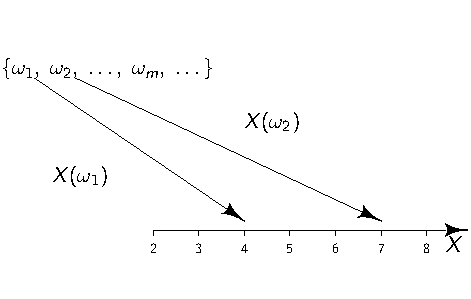
\includegraphics{Resources/Plots/Zahlenzuordnung-1} \end{center}
\normalsize
\end{frame}

\begin{frame}{Eindimensionale Zufallsvariablen}
\phantomsection\label{eindimensionale-zufallsvariablen-5}
\framesubtitle{Zahlenzuordnung}

\begin{itemize}
\item
  Für \[A = \{\omega\in\Omega|X(\omega)\leq x\}\] existiert die
  \hil{Wahrscheinlichkeit} \(P(A)\), die jetzt als die
  Wahrscheinlichkeit für das Ereignis \(\{X\leq x\}\) interpretiert
  werden kann: \[ P(A)=P(\{X\leq x\})=P(X\leq x).\]
\item
  \(X\) überträgt somit auch die Wahrscheinlichkeiten von den
  Ereignissen eines Zufallsexperimentes auf die reellen Zahlen.
\item
  Spezifiziert man so für alle Ereignisse des neuen Stichprobenraumes
  \(X(\Omega)\) die Wahrscheinlichkeiten, erhält man die
  \hil{Wahrscheinlichkeitsverteilung} von \(X\).
\end{itemize}
\end{frame}

\begin{frame}{Eindimensionale Zufallsvariablen}
\phantomsection\label{eindimensionale-zufallsvariablen-6}
\framesubtitle{Zahlenzuordnung}

\xmpl[Münzwurf]Den Stichprobenraum für das \emph{2-malige Werfen einer
Münze} erhält man als
\[\Omega=\{(K,K),(K,Z),(Z,K),(Z,Z)\},\quad Z\textit{: Zahl},  K\text{\textit{: Kopf}}.\]

\(X\) bildet die Ausgänge \(\omega_i,\) \(i=1,\ldots,4\) wie folgt in
die reellen Zahlen ab \begin{equation*}
X = \begin{cases}
0& (K,K)\\
1& (K,Z)\quad\text{oder}\quad(Z,K)\\
2& (Z,Z).
\end{cases}
\end{equation*} \endxmpl
\end{frame}

\begin{frame}{Eindimensionale Zufallsvariablen}
\phantomsection\label{eindimensionale-zufallsvariablen-7}
\framesubtitle{Zahlenzuordnung}

\xmpl[Münzwurf]Als Wertebereich erhält man \(X(\Omega)=\{0,1,2\}\). Für
z.B. \(X(\omega)=0\) lautet das zugehörige Ereignis \(A_1=\{(K,K)\}\).
\(\{X\leq 1\}\) entspricht dem Ereignis \(A_2=\{(K,K),(K,Z),(Z,K)\}\).
\medskip

Ist die Münze fair, sind alle Elementarereignisse gleich wahrscheinlich:
\[P(\{K,K\})=P(\{K,Z\})=P(\{Z,K\})=P(\{Z,Z\})=\frac{1}{4}.\]
\(P(\{X=0\})\) und \(P(\{X\leq 1\})\) ermittelt man dann über \(P(A_1)\)
und \(P(A_2)\):
\[P(X=0)=P(A_1)=\dfrac{1}{4} \quad\text{und}\quad P(X\leq 1)=P(A_2)=\dfrac{3}{4}.\]
\endxmpl
\end{frame}

\begin{frame}{Eindimensionale Zufallsvariablen}
\phantomsection\label{eindimensionale-zufallsvariablen-8}
\framesubtitle{diskrete / stetige Zufallsvariable}

\begin{itemize}
\tightlist
\item
  Ist \(\Omega\) endlich oder abzählbar unendlich, liegt eine
  \hil{diskrete} Zufallsvariable vor.
\item
  Bei einem überabzählbar unendlichen Stichprobenraum kann \(X\) jeden
  beliebigen Zahlenwert eines vorgegebenen Intervalls der reellen Zahlen
  annehmen, wobei auch \((-\infty,\infty)\) zulässig ist.
\item
  Die Zufallsvariable \(X\) nennen wir dann \hil{stetig}.
\end{itemize}
\end{frame}

\begin{frame}{Eindimensionale Zufallsvariablen}
\phantomsection\label{eindimensionale-zufallsvariablen-9}
\framesubtitle{diskrete / stetige Zufallsvariable - QuizAcademy}
\QuizAcademy{Zufallsvariablen 1}\endQuizAcademy
\end{frame}

\begin{frame}{Eindimensionale Zufallsvariablen}
\phantomsection\label{eindimensionale-zufallsvariablen-10}
\framesubtitle{diskrete / stetige Zufallsvariable}

\xmpl[diskrete / stetige Zufallsvariable]\label{xmpl:versp}

\begin{enumerate}
[(a)]
\tightlist
\item
  Ist \(X\) die Anzahl der Würfe einer Münze, bis zum ersten Mal
  \emph{Zahl} oben liegt, sind \(\Omega\) und Wertebereich \(X(\Omega)\)
  abzählbar unendlich.

  \par\medskip

  \(X\) ist daher eine \hil{diskrete} Zufallsvariable mit
  \(X(\omega_i) = x_i=i\) für \(i=1,2\ldots,m,m+1,\ldots\).
\item
  Bei \emph{Verspätung eines Zuges} \(X\) kann bei unendlich genauer
  Zeitmessung jede Verspätung eines Intervalls
  \([x_1,x_2] \subset\mathbb{R}\) eintreten.

  \par\medskip

  \(X\) hat einen überabzählbar unendlichen Wertebereich und ist daher
  \hil{stetig}.
\end{enumerate}

\endxmpl
\end{frame}

\begin{frame}{Eindimensionale Zufallsvariablen}
\phantomsection\label{eindimensionale-zufallsvariablen-11}
\framesubtitle{Lineartransformation}

\begin{itemize}
\tightlist
\item
  Jede auf \(X(\Omega)\) definierte reellwertige Funktion \(g\)
  überführt \(X\) in eine neue Zufallsvariable \(Y=g(X)\).
\item
  Auch \(Y\) liegt der Stichprobenraum \(\Omega\) zugrunde, denn \(Y\)
  stellt eine geschachtelte Funktion dar: \[Y=g[X(\Omega)].\]
\item
  \(X\) sei im Beispiel \ref{xmpl:versp} \blue{(b)} in Minuten gemessen.
  Für die Verspätung in Sekunden resultiert eine Zufallsvariable
  \(Y=60 X\). Ist \(X=3\) (Minuten), folgt \(Y=180\) (Sekunden). Die
  Wahrscheinlichkeit für eine Verspätung zwischen 2 und 3 Minuten ist
  dieselbe wie für eine Verspätung zwischen 120 und 180 Sekunden:
  \[ P(2\leq X\leq3)=P(120\leq Y\leq180).\]
\item
  Man überträgt die Wahrscheinlichkeiten für Ereignisse aus \(\Omega\)
  jetzt auf die Ereignisse von \(Y\).
\end{itemize}
\end{frame}

\begin{frame}{\large Wahrscheinlichkeitsverteilungen von
Zufallsvariablen}
\phantomsection\label{wahrscheinlichkeitsverteilungen-von-zufallsvariablen}
\framesubtitle{Verteilungsfunktion}

\begin{itemize}
\tightlist
\item
  Um z.B. die Wahrscheinlichkeit für Ereignisse der Art
  \[\{X\leq x\},\: \{x_1 < X \leq x_2\},\:\{X=x_1\}\: \text{ oder }\: \{X\neq x_1\}\]
  zu berechnen, ist die \hil{Verteilungsfunktion} hilfreich.
\end{itemize}

\defn[Verteilungsfunktion] \label{VtlgFunktion} Eine Funktion \(F\) mit
\begin{equation} F(x) = P(X\leq x),\quad x\in\mathbb{R},\label{VFunktion}
\end{equation} heißt \hil{Verteilungsfunktion} von \(X\). \enddefn
\end{frame}

\begin{frame}{\large Wahrscheinlichkeitsverteilungen von
Zufallsvariablen}
\phantomsection\label{wahrscheinlichkeitsverteilungen-von-zufallsvariablen-1}
\framesubtitle{Verteilungsfunktion}

\begin{itemize}
\tightlist
\item
  Aufgrund der \hil{Kolmogoroff--Axiome} hat \(F(x)\) folgende
  Eigenschaften:

  \begin{enumerate}
  [(1)]
  \tightlist
  \item
    \(F(x)\) ist \hil{monoton wachsend} mit Werten des Intervalls
    {[}0,1{]}: Gilt \(x_2>x_1\), so folgt daraus \(F(x_2)\geq F(x_1)\).
  \item
    \[\lim_{x\rightarrow-\infty}\limits F(x)=F(-\infty)=0\] und
    \[\lim_{x\rightarrow\infty}\limits F(x)=F(\infty)=1.\]
  \item
    \(F(x)\) ist an jeder Stelle \(x\) \hil{rechtsseitig stetig}, d.h.
    \[\lim_{h\rightarrow 0^+}\limits F(x+h)=F(x).\] Die Notation
    \(h\rightarrow 0^+\) besagt, dass \(h\) mit einem Wert größer 0
    startet und bei der Grenzwertberechnung sich daher von rechts der 0
    nähert.
  \end{enumerate}
\end{itemize}
\end{frame}

\begin{frame}{\large Wahrscheinlichkeitsverteilungen von
Zufallsvariablen}
\phantomsection\label{wahrscheinlichkeitsverteilungen-von-zufallsvariablen-2}
\framesubtitle{Verteilungsfunktion}

\begin{enumerate}
[(1)]
\setcounter{enumi}{3}
\tightlist
\item
  Für jedes Ereignis \(\{x_1<X\leq x_2\}\) gilt
  \[ P(x_1 < X \leq x_2)=P(X \leq x_2) - P(X \leq x_1) = F(x_2) -  F(x_1).\]
\end{enumerate}

\begin{itemize}
\tightlist
\item
  Diese vier allgemeinen Eigenschaften gelten für diskrete und stetige
  Zufallsvariablen.
\item
  Da aber die weitere mathematische Behandlung eine Fallunterscheidung
  verlangt, erfolgt eine getrennte Darstellung.
\end{itemize}
\end{frame}

\begin{frame}{\large Wahrscheinlichkeitsverteilungen von
Zufallsvariablen}
\phantomsection\label{wahrscheinlichkeitsverteilungen-von-zufallsvariablen-3}
\framesubtitle{diskrete Verteilungsfunktion}

\xmpl[Fairer Würfel]Der Wertebereich ist \(X(\Omega)=\{1,2,3,4,5,6\}\)
mit \(P(X=x_i)=\frac{1}{6}\) für \(i=1,\ldots,6\).

Die Verteilungsfunktion \(F(x)\) ist dann \begin{equation*}
F(x)=
\begin{cases}
0& x < 1 \\
\frac{1}{6}& 1 \leq x < 2 \\
\frac{2}{6}& 2 \leq x < 3 \\
\vdots &\\
\frac{5}{6}& 5 \leq x < 6 \\
1& x \geq 6.
\end{cases}
\end{equation*} \endxmpl
\end{frame}

\begin{frame}{\large Wahrscheinlichkeitsverteilungen von
Zufallsvariablen}
\phantomsection\label{wahrscheinlichkeitsverteilungen-von-zufallsvariablen-4}
\framesubtitle{diskrete Verteilungsfunktion}

\xmpl[*]

\footnotesize
\begin{center}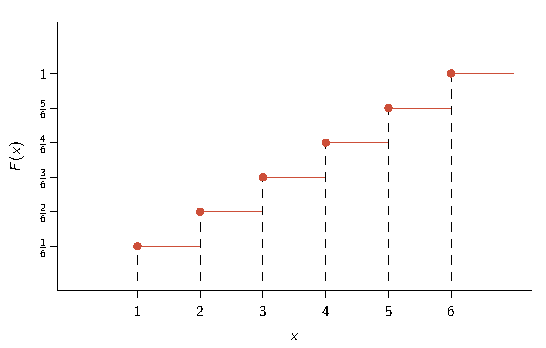
\includegraphics{Resources/Plots/unnamed-chunk-9-1} \end{center}
\normalsize
\endxmpl
\end{frame}

\begin{frame}{\large Wahrscheinlichkeitsverteilungen von
Zufallsvariablen}
\phantomsection\label{wahrscheinlichkeitsverteilungen-von-zufallsvariablen-5}
\framesubtitle{diskrete Verteilungsfunktion}

\begin{itemize}
\tightlist
\item
  Bei diskreten Zufallsvariablen ist \(F(x)\) eine
  \hil{Treppenfunktion}.
\item
  Die Stufenhöhen entsprechen den Wahrscheinlichkeiten für \(X=x_i\).
\item
  Die \hil{Wahrscheinlichkeitsfunktion} \(f(x)\) einer diskreten
  Zufallsvariablen ordnet den \(x_i=X(\omega_i)\) Wahrscheinlichkeiten
  zu.
\item
  \(f(x)\) heißt manchmal auch \hil{Wahrscheinlichkeitsmassefunktion}.
\end{itemize}
\end{frame}

\begin{frame}{\large Wahrscheinlichkeitsverteilungen von
Zufallsvariablen}
\phantomsection\label{wahrscheinlichkeitsverteilungen-von-zufallsvariablen-6}
\framesubtitle{Wahrscheinlichkeitsfunktion}

\defn[Wahrscheinlichkeitsfunktion]Die Funktion
\[f :\; X(\Omega)\longrightarrow\mathbb{R}^+\] mit \begin{equation*}
f(x)=
\begin{cases}
P(X=x_i)=p_i& i=1,2,\ldots \\
0 & \text{sonst}.
\end{cases}
\end{equation*}

heißt \hil{Wahrscheinlichkeitsfunktion} von \(X\) und ordnet jeder
reellen Zahl \(x_i\) die Wahrscheinlichkeit \(P(X=x_i)\) zu.\mps Für
diese gilt \[f(x_i)\geq 0\quad\text{und}\quad \sum_i f(x_i)=1.\]
\enddefn
\end{frame}

\begin{frame}{\large Wahrscheinlichkeitsverteilungen von
Zufallsvariablen}
\phantomsection\label{wahrscheinlichkeitsverteilungen-von-zufallsvariablen-7}
\framesubtitle{Wahrscheinlichkeitsfunktion}

\vspace{1cm}

\xmpl[*]\begin{equation*}
f(x)=
\begin{cases}
P(X=x_i)=p_i=\frac{1}{6}& i=1,\ldots,6\\
0 & \text{sonst}.
\end{cases} 
\end{equation*}

\footnotesize
\normalsize

\endxmpl
\end{frame}

\begin{frame}{\large Wahrscheinlichkeitsverteilungen von
Zufallsvariablen}
\phantomsection\label{wahrscheinlichkeitsverteilungen-von-zufallsvariablen-8}
\framesubtitle{Wahrscheinlichkeitsfunktion}

\begin{align*}
P(x_1< X \leq x_2) & = \sum_{x_1<x_i\leq x_2} f(x_i) = \sum_{x_1<x_i\leq x_2}P(X=x_i) \\
& =\sum_{i:x_1<x_i\leq x_2}p_i.
\end{align*}

\begin{itemize}
\tightlist
\item
  Die Intervallgrenzen \(x_1\) und \(x_2\) sind beliebig; sie müssen
  nicht Elemente von \(X(\Omega)\) sein. Für bspw. \(x_1=1.5\) und
  \(x_2=4.8\) folgt für den \hil{fairen Würfel} \begin{align*}
  P(1.5<X\leq4.8) & = P(X=2)+P(X=3)+P(X=4) \\
                & = p_1+p_2+p_3=\frac{1}{2}.
  \end{align*}
\end{itemize}
\end{frame}

\begin{frame}{\large Wahrscheinlichkeitsverteilungen von
Zufallsvariablen}
\phantomsection\label{wahrscheinlichkeitsverteilungen-von-zufallsvariablen-9}
\framesubtitle{Wahrscheinlichkeitsfunktion}
\exe

Gegeben ist das Zufallsexperiment \emph{dreimaliger Münzwurf einer
unfairen Münze} mit \(P(K)=\frac{1}{3}\) und \(P(Z)=\frac{2}{3}\).

\begin{enumerate}
[(a)]
\tightlist
\item
  Stellen Sie den Stichprobenraum \(\Omega\) und den Wertebereich
  \(X(\Omega)\) für \(X\): \emph{Anzahl Kopf} dar!
\item
  Entwickeln Sie die Wahrscheinlichkeitsfunktion und stellen Sie diese
  grafisch dar!
\item
  Entwickeln Sie die Verteilungsfunktion und stellen Sie diese auch
  grafisch dar!
\end{enumerate}

\endexe
\end{frame}

\begin{frame}{\large Wahrscheinlichkeitsverteilungen von
Zufallsvariablen}
\phantomsection\label{wahrscheinlichkeitsverteilungen-von-zufallsvariablen-10}
\framesubtitle{Wahrscheinlichkeitsfunktion}
\vspace{1cm}

\exe

Für Zufallsvariable \(X\): \emph{Anzahl der Autoverkäufe pro Tag} gilt:

\begin{center}
\begin{tabular}{|c|cccccc|}\hline
$X$   & 0 & 1 & 2 & 3 & 4 & 5\\\hline
$f(x)$& 0.18 & 0.39 & 0.24 & 0.14 & 0.04 & 0.01\\
$F(x)$& 0.18 & 0.57 & 0.81 & 0.95 & 0.99 & 1\\\hline
\end{tabular}
\end{center}

Wie groß ist die Wahrscheinlichkeit, dass

\begin{enumerate}
[(a)]
\tightlist
\item
  am Tag ein Auto verkauft wird?
\item
  am Tag höchstens 2 Autos verkauft werden?
\item
  am Tag mehr als 2, aber höchstens 4 Autos verkauft werden?
\item
  am Tag mindestens 2, aber höchstens 4 Autos verkauft werden?
\end{enumerate}

\endexe
\end{frame}

\begin{frame}{\large Wahrscheinlichkeitsverteilungen von
Zufallsvariablen}
\phantomsection\label{wahrscheinlichkeitsverteilungen-von-zufallsvariablen-11}
\framesubtitle{Wahrscheinlichkeitsdichte}

\begin{itemize}
\tightlist
\item
  Eine \hil{stetige Zufallsvariable} kann jeden Wert eines Intervalls
  der reellen Zahlen annehmen.
\item
  \(P(X\leq x)\) resultiert hier wegen der überabzählbar unendlich
  vielen Realisationen von \(X\) durch \hil{Integration} einer
  geeigneten Funktion \(f(x)\).
\item
  Da \(-\infty<X<\infty\) das sichere Ereignis ist, muss gelten:
  \[f(x)\geq 0\quad\text{und}\quad P(-\infty<X<\infty)=\int^\infty_{-\infty}\limits f(x)\, dx=1.\]
  Derartige Funktionen heißen \hil{Dichtefunktionen}.
\end{itemize}
\end{frame}

\begin{frame}{\large Wahrscheinlichkeitsverteilungen von
Zufallsvariablen}
\phantomsection\label{wahrscheinlichkeitsverteilungen-von-zufallsvariablen-12}
\framesubtitle{Wahrscheinlichkeitsdichte}

\defn[Dichtefunktion] \label{DichteFkt} Eine Funktion
\(f:\; X(\Omega)\longrightarrow\mathbb{R}^+\) heißt
\hil{Wahrscheinlichkeitsdichte} oder \hil{Dichtefunktion}, wenn gilt
\[ F(x)=P(X\leq x) = \int_{-\infty}^x\limits f(u)\, du \quad \text{für jedes } x\in\mathbb{R}.\]
\enddefn
\end{frame}

\begin{frame}{\large Wahrscheinlichkeitsverteilungen von
Zufallsvariablen}
\phantomsection\label{wahrscheinlichkeitsverteilungen-von-zufallsvariablen-13}
\framesubtitle{Wahrscheinlichkeitsdichte}

\vspace{1cm}

\begin{itemize}
\tightlist
\item
  Für alle Werte von \(x\), in denen \(F(x)\) differenzierbar ist,
  erhält man \[\frac{d F(x)}{dx} = f(x);\] d.h. die Dichtefunktion ist
  die erste Ableitung der Verteilungsfunktion.
\item
  Die Wahrscheinlichkeit für ein Ereignis \((x_1<X\leq x_2)\) ist dann
  \begin{align*}
  P(x_1<X\leq x_2) & = F(x_2) - F(x_1) = \int^{x_2}_{-\infty}\limits
  f(x)\, dx - \int^{x_1}_{-\infty}\limits f(x)\, dx \\
  & = \int^{x_2}_{x_1}\limits f(x)\, dx.
  \end{align*}
\end{itemize}
\end{frame}

\begin{frame}{\large Wahrscheinlichkeitsverteilungen von
Zufallsvariablen}
\phantomsection\label{wahrscheinlichkeitsverteilungen-von-zufallsvariablen-14}
\framesubtitle{Wahrscheinlichkeitsdichte}

\footnotesize
\begin{center}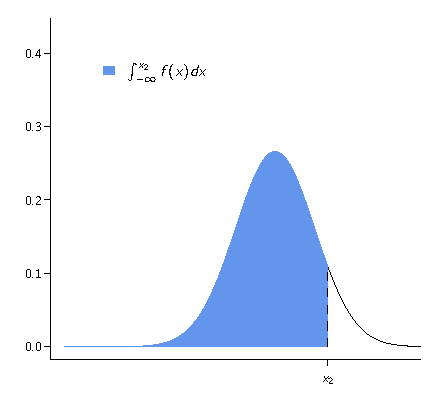
\includegraphics{Resources/Plots/Wahrscheinlichkeitsdichte-1} 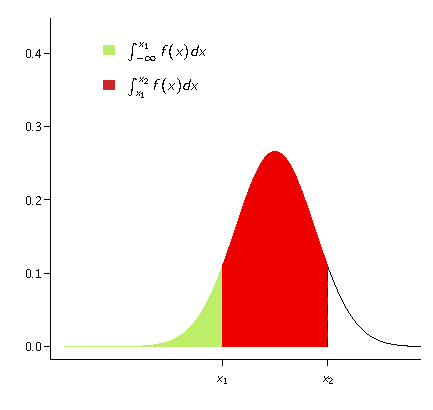
\includegraphics{Resources/Plots/Wahrscheinlichkeitsdichte-2} \end{center}
\normalsize
\end{frame}

\begin{frame}{\large Wahrscheinlichkeitsverteilungen von
Zufallsvariablen}
\phantomsection\label{wahrscheinlichkeitsverteilungen-von-zufallsvariablen-15}
\framesubtitle{Wahrscheinlichkeitsdichte}
\vspace{1cm}

\begin{itemize}
\tightlist
\item
  Für einen einzelnen Wert gilt also im stetigen Fall,
  dass\[P(X=x_1) =\int^{x_1}_{x_1}\limits f(x)\, dx=0\] für beliebiges
  \(x_1\).
\item
  Das heißt aber nicht, dass diese Ereignisse unmöglich sind! Vielmehr
  zeigt es, dass \(f(x)\) im stetigen Fall nicht die Wahrscheinlichkeit
  für \(X=x\) angibt.
\item
  Daher ist auch möglich, dass für einige Werte \(f(x)>1\) gilt.
\item
  Da im stetigen Fall immer gilt \(P(X=x)=0\), stimmen folgende
  Wahrscheinlichkeiten überein: \begin{align*}
  P(x_1\leq X\leq x_2) & = P(x_1<X\leq x_2)=P(x_1\leq X<x_2) \\
  & = P(x_1<X<x_2).
  \end{align*}
\end{itemize}
\end{frame}

\begin{frame}{\large Wahrscheinlichkeitsverteilungen von
Zufallsvariablen}
\phantomsection\label{wahrscheinlichkeitsverteilungen-von-zufallsvariablen-16}
\framesubtitle{Verteilungs- und Dichtefunktion}

\xmpl[Berechnung von Wahrscheinlichkeiten bei stetigen ZV]Eine stetige
Zufallsvariable \(X\) hat die Verteilungsfunktion \begin{equation*}
F(x)=
\begin{cases}
0  &  x \leq 0 \\
\frac{1}{8}x^3  & 0 < x < 2\\
1 & x \geq 2.
\end{cases}
\end{equation*} Da \(F(x)\) über den drei Teilintervallen
differenzierbar ist, ist die Dichtefunktion die Ableitung von \(F(x)\):
\begin{equation*}
 f(x) =
 \begin{cases}
  \frac{3}{8}x^2 & 0 < x \leq 2 \\
  0 & \text{sonst}.
  \end{cases}
\end{equation*} \endxmpl
\end{frame}

\begin{frame}{\large Wahrscheinlichkeitsverteilungen von
Zufallsvariablen}
\phantomsection\label{wahrscheinlichkeitsverteilungen-von-zufallsvariablen-17}
\framesubtitle{Verteilungs- und Dichtefunktion - QuizAcademy}
\QuizAcademy{Zufallsvariablen 2}\endQuizAcademy
\end{frame}

\begin{frame}{\large Wahrscheinlichkeitsverteilungen von
Zufallsvariablen}
\phantomsection\label{wahrscheinlichkeitsverteilungen-von-zufallsvariablen-18}
\framesubtitle{Verteilungs- und Dichtefunktion}

\xmpl[Berechnung von Wahrscheinlichkeiten bei stetigen ZV]\(P(1<X\leq\frac{3}{2})\)
lässt sich über \(F(x)\) und \(f(x)\) berechnen:
\[ P\left(1<X\leq\frac{3}{2}\right)=F\left(\frac{3}{2}\right) -F(1)=\frac{27}{64}-\frac{1}{8}=\frac{19}{64};\]
aber auch
\[\int^{\frac{3}{2}}_1\limits \frac{3}{8} x^2 \, dx =\frac{1}{8}x^3 \bigg|^{\frac{3}{2}}_1 =\frac{27}{64}-\frac{1}{8}=\frac{19}{64}.\]
Die folgenden Grafiken zeigen beide Funktionen. \endxmpl
\end{frame}

\begin{frame}{\large Wahrscheinlichkeitsverteilungen von
Zufallsvariablen}
\phantomsection\label{wahrscheinlichkeitsverteilungen-von-zufallsvariablen-19}
\framesubtitle{Verteilungs- und Dichtefunktion}

Abbildung (a) gibt die Wahrscheinlichkeit als Differenz der beiden
Funktionswerte, Abbildung (b) als Flächeninhalt wieder. \xmpl[*]

\footnotesize
\begin{center}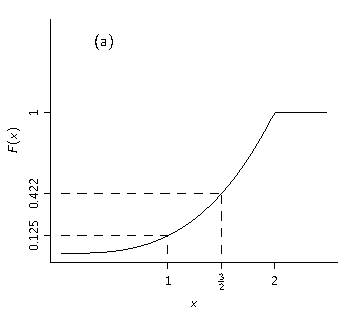
\includegraphics{Resources/Plots/unnamed-chunk-10-1} 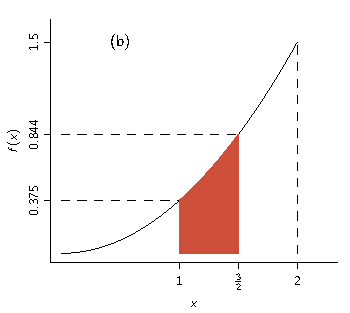
\includegraphics{Resources/Plots/unnamed-chunk-10-2} \end{center}
\normalsize
\endxmpl
\end{frame}

\begin{frame}[fragile]{\large Wahrscheinlichkeitsverteilungen von
Zufallsvariablen}
\phantomsection\label{wahrscheinlichkeitsverteilungen-von-zufallsvariablen-20}
\framesubtitle{Verteilungs- und Dichtefunktion in \R}

\footnotesize

\begin{Shaded}
\begin{Highlighting}[]
\CommentTok{\# Verteilungsfunktion definieren}
\NormalTok{myCdf }\OtherTok{\textless{}{-}} \ControlFlowTok{function}\NormalTok{(x) \{}
  \ControlFlowTok{if}\NormalTok{(x }\SpecialCharTok{\textless{}} \DecValTok{0}\NormalTok{)\{                    }\CommentTok{\# Wenn x \textless{} 0,}
\NormalTok{    cdf }\OtherTok{\textless{}{-}} \DecValTok{0}                    \CommentTok{\# dann nimmt cdf den Wert 0 an.}
\NormalTok{  \} }\ControlFlowTok{else} \ControlFlowTok{if}\NormalTok{(x }\SpecialCharTok{\textgreater{}=} \DecValTok{0} \SpecialCharTok{\&}\NormalTok{ x }\SpecialCharTok{\textless{}=} \DecValTok{2}\NormalTok{)\{   }\CommentTok{\# Sonst, wenn 0 \textless{}= x \textless{}= 2,}
\NormalTok{    cdf }\OtherTok{\textless{}{-}} \FloatTok{0.125}\SpecialCharTok{*}\NormalTok{x}\SpecialCharTok{\^{}}\DecValTok{3}            \CommentTok{\# dann berechne die cdf mit 0.125*x\^{}3.}
\NormalTok{  \} }\ControlFlowTok{else}\NormalTok{ \{}
\NormalTok{    cdf }\OtherTok{\textless{}{-}} \DecValTok{1}                    \CommentTok{\# Sonst nimmt cdf den Wert 1 an.}
\NormalTok{  \}}
\NormalTok{  cdf}
\NormalTok{\}}

\CommentTok{\# Dichtefunktion definieren}
\NormalTok{myPdf }\OtherTok{\textless{}{-}} \ControlFlowTok{function}\NormalTok{(x) }\FunctionTok{ifelse}\NormalTok{(x }\SpecialCharTok{\textgreater{}} \DecValTok{0} \SpecialCharTok{\&}\NormalTok{ x }\SpecialCharTok{\textless{}=} \DecValTok{2}\NormalTok{, .}\DecValTok{375} \SpecialCharTok{*}\NormalTok{ x}\SpecialCharTok{\^{}}\DecValTok{2}\NormalTok{, }\DecValTok{0}\NormalTok{)}

\FunctionTok{myCdf}\NormalTok{(}\FloatTok{1.5}\NormalTok{) }\SpecialCharTok{{-}} \FunctionTok{myCdf}\NormalTok{(}\DecValTok{1}\NormalTok{)}
\end{Highlighting}
\end{Shaded}

\begin{verbatim}
## [1] 0.2969
\end{verbatim}

\begin{Shaded}
\begin{Highlighting}[]
\FunctionTok{integrate}\NormalTok{(}\AttributeTok{f =}\NormalTok{ myPdf, }\AttributeTok{lower =} \DecValTok{1}\NormalTok{, }\AttributeTok{upper =} \FloatTok{1.5}\NormalTok{)}
\end{Highlighting}
\end{Shaded}

\begin{verbatim}
## 0.2969 with absolute error < 3.3e-15
\end{verbatim}

\normalsize
\end{frame}

\begin{frame}{\large Wahrscheinlichkeitsverteilungen von
Zufallsvariablen}
\phantomsection\label{wahrscheinlichkeitsverteilungen-von-zufallsvariablen-21}
\framesubtitle{Verteilungs- und Dichtefunktion}
\exe

Für die Zufallsvariable \(X\) gilt \[f(x)=\left\{\begin{array}{ll}
\frac{1}{2}x & 0\leq x\leq 2\\[2mm]
0 & \text{sonst}.
\end{array}\right.\]

\begin{enumerate}
[(a)]
\tightlist
\item
  Zeigen Sie, dass \(f(x)\) eine Dichtefunktion ist und stellen Sie
  diese grafisch dar!
\item
  Berechnen Sie die Verteilungsfunktion und stellen Sie diese grafisch
  dar!
\item
  Bestimmen Sie die folgenden Wahrscheinlichkeiten:
\end{enumerate}

\begin{center}
\begin{tabular}{ll}
\blue{(i)} $P(X=1)$ & \blue{(ii)} $P(X\leq 1)$ \\[2mm]
\blue{(iii)} $P(\frac{1}{2}\leq X\leq\frac{3}{2})$   & \blue{(iv)} $P(\frac{1}{2}< X\leq\frac{3}{2})$ 
\end{tabular}
\end{center}
\endexe
\end{frame}

\begin{frame}{\large Wahrscheinlichkeitsverteilungen von
Zufallsvariablen}
\phantomsection\label{wahrscheinlichkeitsverteilungen-von-zufallsvariablen-22}
\framesubtitle{Verteilungs- und Dichtefunktion}
\exe

Die Zufallsvariable \(X\) hat die folgende Verteilungsfunktion
\[F(x)=\left\{\begin{array}{ll}
0 & x\leq0\\
\frac{1}{27}(x-3)^3+1 & 0<x<3\\
1 & x\geq3.\end{array}\right.\] Bestimmen Sie die Dichtefunktion!
\endexe
\end{frame}

\begin{frame}{Parameter von Verteilungen}
\phantomsection\label{parameter-von-verteilungen}
\framesubtitle{Analogie zur deskriptiven Statistik}

\begin{itemize}
\tightlist
\item
  Wie in der deskriptiven Statistik lassen sich \hil{Parameter} zur
  Charakterisierung von jetzt Wahrscheinlichkeitsverteilungen
  entwickeln.
\item
  Die wichtigsten Maßzahlen zur Beschreibung von Verteilungen sind
  \hil{Lage- und Streuungsparameter}.
\item
  Die zentrale Stellung des arithmetischen Mittels in der deskriptiven
  Statistik nimmt in der Wahrscheinlichkeitstheorie der
  \hil{Erwartungswert} ein.
\item
  Der mit E symbolisierte Erwartungswert soll zunächst an einem Beispiel
  erläutert werden.
\end{itemize}
\end{frame}

\begin{frame}{Parameter von Verteilungen}
\phantomsection\label{parameter-von-verteilungen-1}
\framesubtitle{Erwartungswert}

\xmpl[Glücksspiel]Für einen Einsatz von 2€ darf man einen fairen Würfel
einmal werfen. Die Hälfte der geworfenen Augenzahl wird (in €)
ausgezahlt.

\par\medskip

Welchen Gewinn kann ein Spieler erwarten?

\begin{itemize}
\tightlist
\item
  Die Auszahlungen transformieren die diskrete Zufallsvariable
  \(X=\{1,2,3,4,5,6\}\) in eine neue Zufallsvariable mit Wertebereich
  \[\left\{\frac{1}{2},1,\frac{3}{2},2,\frac{5}{2},3\right\}.\]
\item
  Berücksichtigt man die Einsatzkosten von 2€, erhält man als mögliche
  Gewinne
  \[\left\{-\frac{3}{2},-1,-\frac{1}{2},0,\frac{1}{2},1\right\}.\]
\end{itemize}

\endxmpl
\end{frame}

\begin{frame}{Parameter von Verteilungen}
\phantomsection\label{parameter-von-verteilungen-2}
\framesubtitle{Erwartungswert}
\xmpl[Glücksspiel]

\begin{itemize}
\tightlist
\item
  Diese Werte sind die Realisationen der neuen Zufallsvariablen
  \[Y=g(X)=\frac{1}{2} X-2.\]
\item
  Jeder Ausgang \(y_i \in Y\) tritt ein mit Wahrscheinlichkeit
  \[P(Y=y_i)=P(X=x_i)=\frac{1}{6}.\]
\item
  Der zu erwartende Gewinn ergibt sich intuitiv, indem jeder mögliche
  Ausgang mit seiner Eintrittswahrscheinlichkeit gewichtet wird:
  \[\E(Y)=\left(-\frac{3}{2}\right)\cdot \frac{1}{6}+\left(-1\right)\cdot\frac{1}{6}+ \left(-\frac{1}{2}\right)\cdot \frac{1}{6} + 0 \cdot \frac{1}{6}+\frac{1}{2}\cdot \frac{1}{6}+ 1 \cdot \frac{1}{6}=-0.25.\]
  \vspace{-0.5cm}
\end{itemize}

\endxmpl
\end{frame}

\begin{frame}{Parameter von Verteilungen}
\phantomsection\label{parameter-von-verteilungen-3}
\framesubtitle{Erwartungswert}

Sei \(g(x)\) eine auf \(X(\Omega)\) definierte reellwertige Funktion.
\defn[Erwartungswert einer diskreten Zufallsvariable]Sei \(X\) eine
\hil{diskrete} Zufallsvariable mit der Wahrscheinlichkeitsfunktion
\(f(x_i)\). \linebreak Falls \(\sum |g(x_i)|f(x_i)<\infty\), ist der
\hil{Erwartungswert} von \(g(X)\) gegeben als
\[ \E[g(X)]=\sum^m_{i=1}g(x_i)f(x_i).\] \enddefn
\defn[Erwartungswert einer stetigen Zufallsvariable]Sei \(X\) eine
\hil{stetige} Zufallsvariable mit Dichtefunktion \(f(x)\).
\linebreak Falls \(\int^\infty_{-\infty}|g(x)|f(x)\, dx<\infty\), so ist
der \hil{Erwartungswert} von \(g(X)\) gegeben als
\[ \E[g(X)]=\int^\infty_{-\infty}\limits g(x)f(x)\, dx.\] \enddefn
\end{frame}

\begin{frame}{Parameter von Verteilungen}
\phantomsection\label{parameter-von-verteilungen-4}
\framesubtitle{Erwartungswert}

\begin{itemize}
\tightlist
\item
  Das Integral in der vorangegangenen Definition bezieht sich auf den
  größtmöglichen \hil{Wertebereich} von \(X\).
\item
  Falls die Dichtefunktion nur über einem Intervall \(a\leq X\leq b\)
  Werte größer als null annimmt, erfolgt die Integration über diesem
  Intervall.
\item
  Für \(g(X)=X^{\alpha}\), \(\alpha \in \mathbb{N}\) heißt der
  Erwartungswert \hil{Anfangsmoment}
  \hil{der Ordnung {\boldmath{$\alpha$}}}:
  \begin{equation}\label{Anfangsmomente}
  \E(X^\alpha)=
  \begin{cases}
  \sum_{i=1}^m x_i^\alpha f(x_i) &  X\text{: diskret} \\[1ex]
  \int_{-\infty}^\infty x^\alpha f(x)\, dx & X\text{: stetig}.
  \end{cases}
  \end{equation}
\end{itemize}
\end{frame}

\begin{frame}{Parameter von Verteilungen}
\phantomsection\label{parameter-von-verteilungen-5}
\framesubtitle{Erwartungswert}

\defn[Erwartungswert einer Zufallsvariablen ($\alpha=1$)]
 Der Erwartungswert einer Zufallsvariablen \(X\) ist definiert als
\begin{equation*}
  \E(X)=\mu=
  \begin{cases}
   \sum_{i=1}^m  x_i f(x_i) & X\text{: diskret} \\[1ex]
   \int_{-\infty}^\infty x f(x) \, dx &  X\text{: stetig}.
  \end{cases}
 \end{equation*} \enddefn

\xmpl[Erwartungswert - diskreter Fall]Der Erwartungswert beim Werfen
eines fairen Würfels beträgt
\[\E(X)=\sum^m_{i=1} x_i f(x_i)=\sum^m_{i=1} x_ip_i=1\cdot\frac{1}{6}+2\cdot\frac{1}{6}+\ldots+6\cdot\frac{1}{6}=3.5. \label{EWWuerfel}\]
Man sieht an diesem Ergebnis, dass der Erwartungswert diskreter
Zufallsvariablen keine Realisation von \(X\) sein muss. \endxmpl
\end{frame}

\begin{frame}{Parameter von Verteilungen}
\phantomsection\label{parameter-von-verteilungen-6}
\framesubtitle{Erwartungswert}

\xmpl[Roulette]Beim Roulette kann man auf Zahlen \((0,1,2,\ldots,36)\)
oder Farben (rot und schwarz) setzen. Wird die Farbe richtig
vorhergesagt, ist der Gewinn gleich der Höhe des Einsatzes. Jeweils 18
Zahlen sind rot sowie schwarz (die Null hat keine Farbe).

\par

Setzt man also 10€ auf rot, beträgt der erwartete Gewinn
\[\E(X)=10\cdot\frac{18}{37}+\left(-10\right)\cdot\frac{19}{37}=-0.2703.\]
\endxmpl
\end{frame}

\begin{frame}{Parameter von Verteilungen}
\phantomsection\label{parameter-von-verteilungen-7}
\framesubtitle{Erwartungswert}

\xmpl[Erwartungswert - stetiger Fall]Als Erwartungswert der stetigen
Zufallsvariablen mit \(f(x)=\frac{3}{8}x^2,\) \(0<x\leq 2\) erhält man
\begin{align} 
\E(X)=\int^2_0\limits xf(x)\, dx = \int^2_0\limits x\frac{3}{8}x^2\, dx= \int^2_0\limits \frac{3}{8}x^3\, dx=\frac{3}{32}x^4 \Bigg|^2_0 =\frac{3}{2}.
\label{stetExpBsp}\end{align} \endxmpl
\end{frame}

\begin{frame}{Parameter von Verteilungen}
\phantomsection\label{parameter-von-verteilungen-8}
\framesubtitle{Rechenregeln für den Erwartungswert}

\begin{itemize}
\tightlist
\item
  Für den \hil{Erwartungswertoperator} \(\E\) gelten unabhängig davon,
  ob \(X\) diskret oder stetig ist, folgende Regeln für alle
  \(a,b \in \mathbb{R}\): \begin{eqnarray}
  & \text{\blue{(a)}}& \E(a) = a, \label{EKst} \\
  & \text{\blue{(b)}}& \E(a+bX)=a+b\E(X), \label{ElinTrafo} \\
  & \text{\blue{(c)}}& \E\left[\sum^n_{j=1}\limits c_jg_j(X)\right] = \sum^n_{j=1}\limits
  c_j\E[g_j(X)] = c_1 \E[g_1(X)]+\ldots+c_n \E[g_n(X)], \notag
  \end{eqnarray} falls \(g_j\) eine stetige Funktion für alle
  \(j=1,\ldots,n\) ist. Für deren Herleitungen siehe Buch S.~69 ff.
\end{itemize}
\end{frame}

\begin{frame}{Parameter von Verteilungen}
\phantomsection\label{parameter-von-verteilungen-9}
\framesubtitle{arithmetisches Mittel und Erwartungswert}

\begin{itemize}
\tightlist
\item
  Der Erwartungswert einer diskreten Zufallsvariablen stimmt formal mit
  dem \hil{arithmetischen Mittel} \[\bar{x}=\sum^m_{i=1}\limits x_ih_i\]
  überein, wobei \(h_i\) die relative Häufigkeit der \(i\)-ten
  Merkmalsausprägung im Datensatz bezeichnet.
\item
  Trotz der formalen Übereinstimmung besteht zwischen beiden Maßzahlen
  ein erheblicher Unterschied, dessen Beachtung für ein genaues
  Verständnis beider Konzepte bedeutsam ist.
\item
  Der Erwartungswert \(\E(X)\) charakterisiert die Verteilung einer
  Zufallsvariablen gemäß der statistischen
  Wahrscheinlichkeitsdefinition.
\item
  Dieser Wert bedarf keiner tatsächlichen Durchführungen und ist von
  diesen unabhängig.
\end{itemize}
\end{frame}

\begin{frame}{Parameter von Verteilungen}
\phantomsection\label{parameter-von-verteilungen-10}
\framesubtitle{arithmetisches Mittel und Erwartungswert}

\begin{itemize}
\tightlist
\item
  Das arithmetische Mittel hingegen kennzeichnet den durchschnittlichen
  Wert eines Datensatzes, d.h. es müssen Beobachtungen vorliegen.
\item
  Wird ein Experiment \(n\)-mal durchgeführt, so liegen die
  \hil{Realisationen} \(x_1,\ldots,x_n\) von \(X\) vor, für die das
  arithmetische Mittel \[\bar{x}=\dfrac{1}{n}\sum\limits^n_{j=1}x_j\]
  berechnet werden kann.
\item
  Das arithmetische Mittel kennzeichnet jetzt den Datensatz, nicht
  jedoch \(\E(X)\).
\item
  Erhöht man \(n\), wird sich \(\bar{x}\) \(\E(X)\) annähern. Dazu
  später mehr.
\end{itemize}
\end{frame}

\begin{frame}{Parameter von Verteilungen}
\phantomsection\label{parameter-von-verteilungen-11}
\framesubtitle{Varianz und Standardabweichung}

\begin{itemize}
\tightlist
\item
  \hil{Varianz} bzw. \hil{Standardabweichung} quantifizieren die
  \hil{Streuung} einer Verteilung.
\item
  Auch die Varianz ergibt sich für eine spezielle Funktion \(g(X)\) aus
  den Definitionen für den Erwartungswert. Für \(g(X)=(X-\mu)^\alpha,\)
  \(\alpha\in \mathbb{N}\), heißt der Erwartungswert \begin{equation*}
  \E[(X-\mu)^\alpha] =
  \begin{cases}
   \sum_{i=1}^m (x_i-\mu)^\alpha f(x_i) & X\text{: diskret} \\[1ex]
   \int_{-\infty}^\infty (x-\mu)^\alpha f(x) \, dx & X\text{: stetig}
  \end{cases}
   \end{equation*}
  \hil{Zentralmoment der Ordnung {\boldmath{$\alpha$}}}.
\item
  Für \(\alpha=2\) resultiert die Varianz als Zentralmoment zweiter
  Ordnung: \[ \var(X) = \E[(X-\mu)^2] = \sigma^2.\]
\end{itemize}
\end{frame}

\begin{frame}{Parameter von Verteilungen}
\phantomsection\label{parameter-von-verteilungen-12}
\framesubtitle{Varianz und Standardabweichung}
\vspace{1cm}

\defn[Standardabweichung]Die \hil{Standardabweichung} \(\sigma\) ist
definiert als \(\sigma =\sqrt{\sigma^2}\). \enddefn
\defn[Varianz: Spezieller Verschiebungssatz]Die Varianz kann durch
Anfangsmomente dargestellt werden:
\[ \sigma^2=\E[(X-\mu)^2]=\E(X^2)-2\mu
\E(X)+\E(\mu^2).\] Die rechte Seite der Gleichung lässt sich
zusammenfassen zu \begin{equation}\label{VerschSatzVar}
\sigma^2=\E(X^2)-[\E(X)]^2=\E(X^2)-\mu^2.
\end{equation} \(\E(X^2)\) ist das Anfangsmoment zweiter Ordnung,
\([\E(X)]^2\) das Quadrat des Anfangsmoments erster Ordnung. \enddefn
\end{frame}

\begin{frame}{Parameter von Verteilungen}
\phantomsection\label{parameter-von-verteilungen-13}
\framesubtitle{Varianz und Standardabweichung}

\xmpl[Varianz - diskreter Fall]Die Varianz beim Werfen eines fairen
Würfels beträgt
\[\sigma^2=\E(X^2)-[\E(X)]^2=\sum^m_{i=1}\limits x_i^2f(x_i)-\mu^2=1^2\cdot\frac{1}{6}+\ldots+6^2\cdot\frac{1}{6}-3.5^2=2.9167 \label{VarWuerfel}.\]
Standardabweichung: \(\sigma=\sqrt{\sigma^2}=1.7078\). \endxmpl
\xmpl[Roulette]Setzt man also 10€ auf rot, beträgt die Varianz
\[\sigma^2=\E(X^2)-[\E(X)]^2=10^2\cdot\frac{18}{37}+\left(-10\right)^2\cdot\frac{19}{37}-\left(-0.2703\right)^2=99.927.\]
Standardabweichung: \(\sigma=\sqrt{\sigma^2}=9.9963\). \endxmpl
\end{frame}

\begin{frame}{Parameter von Verteilungen}
\phantomsection\label{parameter-von-verteilungen-14}
\framesubtitle{Varianz und Standardabweichung}

\xmpl[Varianz - stetiger Fall]Als Varianz der stetigen Zufallsvariablen
mit \(f(x)=\frac{3}{8}x^2,\) \(0<x\leq 2\) erhält man
\begin{eqnarray}\notag
\sigma^2=\E(X^2)-[\E(X)]^2&=&\int^2_0\limits x^2f(x)\, dx-\left[\int^2_0\limits xf(x)\, dx\right]^2\\
&=& \int^2_0\limits x^2\frac{3}{8}x^2\, dx-\left[\int^2_0\limits x\frac{3}{8}x^2\, dx\right]^2\\
& \stackrel{\eqref{stetExpBsp}}{=} & \int^2_0\limits\frac{3}{8}x^4\, dx-\left(\frac{3}{2}\right)^2\\
&=&\frac{3}{40}x^5 \Bigg|^2_0-\frac{9}{4} =\frac{12}{5}-\frac{9}{4}=\frac{3}{20}.\label{stetVarBsp}
\end{eqnarray} \endxmpl
\end{frame}

\begin{frame}{Parameter von Verteilungen}
\phantomsection\label{parameter-von-verteilungen-15}
\framesubtitle{Rechenregeln für die Varianz}

Für die Varianz gelten die folgenden Regeln: \begin{eqnarray}
  \var(a) & = & 0 \label{varKst}\\
  \var(a+bX) & = & b^2 \var(X)\label{varlinTrafo}
  \end{eqnarray} für Konstanten \(a,b \in \mathbb{R}\).

Ergebnis \eqref{varlinTrafo} weisen wir in \eqref{VarLinKomb3} nach.
\end{frame}

\begin{frame}{Parameter von Verteilungen}
\phantomsection\label{parameter-von-verteilungen-16}
\framesubtitle{Erwartungswert und Varianz - QuizAcademy}
\QuizAcademy{Zufallsvariablen 3}\endQuizAcademy
\end{frame}

\begin{frame}{Parameter von Verteilungen}
\phantomsection\label{parameter-von-verteilungen-17}
\framesubtitle{Erwartungswert und Varianz}
\exe

Berechnen Sie \blue{(a)} den Erwartungswert und \blue{(b)} die Varianz
bzw. die Standardabweichung für die diskrete Zufallsvariable \(X\):
\emph{Anzahl der Autoverkäufe pro Tag}

\begin{center}
\begin{tabular}{|c|cccccc|}\hline
$X$   & 0 & 1 & 2 & 3 & 4 & 5\\\hline
$f(x)$& 0.18 & 0.39 & 0.24 & 0.14 & 0.04 & 0.01\\
$F(x)$& 0.18 & 0.57 & 0.81 & 0.95 & 0.99 & 1\\\hline
\end{tabular}
\end{center}
\endexe
\exe

Berechnen Sie \blue{(a)} den Erwartungswert und \blue{(b)} die Varianz
bzw. die Standardabweichung für die stetige Variable \(X\) mit der
Dichtefunktion
\[f(x)=\left\{\begin{array}{ll}-\frac{1}{72}x^2+\frac{1}{12}x+\frac{1}{12} & 0\leq x\leq 6\\ 
0 & \text{sonst}.\end{array}\right.\] \endexe
\end{frame}

\begin{frame}{Parameter von Verteilungen}
\phantomsection\label{parameter-von-verteilungen-18}
\framesubtitle{Erwartungswert und Varianz}
\exe

Für die diskrete Zufallsvariable \(X\) ist folgende
Wahrscheinlichkeitsfunktion gegeben
\[f(x)=\left\{\begin{array}{ll} 0.1& x=-1\\
                               0.3& x=0\\
                               0.6& x=1\\
                               0& \text{sonst}.\end{array}\right.\]

\begin{enumerate}
[(i)]
\tightlist
\item
  Berechnen Sie \blue{(a)} den Erwartungswert und \blue{(b)} die Varianz
  bzw. die Standardabweichung für \(X\)!
\item
  Berechnen Sie \blue{(a)} den Erwartungswert und \blue{(b)} die Varianz
  bzw. die Standardabweichung für \(Y=2X^2+1\)!
\end{enumerate}

\endexe
\end{frame}

\begin{frame}{Linearkombination}
\phantomsection\label{linearkombination}
\framesubtitle{Drei Spezifikationen}

Mehrere Zufallsvariablen, die entweder alle diskret oder alle stetig
sind, können zu einer neuen Zufallsvariablen verknüpft werden.

\defn[Linearkombination]Gegeben seien die Zufallsvariablen
\(X_1, X_2,\ldots,X_n\) und Konstanten
\[\lambda_1, \lambda_2,\ldots,\lambda_n.\] Die Zufallsvariable
\[Y=\lambda_1X_1+\lambda_2X_2+\ldots+\lambda_nX_n =
  \sum\limits^n_{j=1}\lambda_jX_j\] heißt \hil{Linearkombination} der
Zufallsvariablen \(X_j\), \(j=1,\ldots,n\). \enddefn
\end{frame}

\begin{frame}{Linearkombination}
\phantomsection\label{linearkombination-1}
\framesubtitle{Drei Spezifikationen}

Besonders wichtige Linearkombinationen sind die folgenden: \medskip

\begin{enumerate}
[(1)]
\tightlist
\item
  Sind alle \(\lambda_j=1\), erhält man die \hil{Summe} der \(n\)
  Zufallsvariablen \(X_j\), \begin{equation*}
  \tilde{S}=X_1+X_2+\ldots+X_n = \sum\limits^n_{j=1} X_j.
  \end{equation*}
\item
  Für \(\lambda_j=1/n\) resultiert das \hil{arithmetische Mittel} der
  \(X_j\), \begin{equation*}
   \bar{X}=\frac{1}{n}X_1+\frac{1}{n}X_2+\ldots+\frac{1}{n}X_n=\frac{1}{n}
  \sum\limits^n_{j=1}X_j = \frac{1}{n}\tilde{S}.
  \end{equation*}
\item
  \(\lambda_j=0\) für \(j=3,\ldots,n\) und \(X_2=1\) liefert eine
  \hil{Lineartransformation} \begin{equation*}
    Y=\lambda_1X_1+\lambda_2,
    \end{equation*} da \(Y\) eine lineare Funktion von \(X_1\) ist.
\end{enumerate}
\end{frame}

\begin{frame}{Linearkombination}
\phantomsection\label{linearkombination-2}
\framesubtitle{Erwartungswert und Varianz - Rechenregeln}

\begin{itemize}
\tightlist
\item
  Bei der Varianzberechnung muss unterschieden werden, ob die
  Zufallsvariablen \(X_j\) paarweise stochastisch unabhängig sind oder
  nicht.
\item
  Es sei hier zunächst \hil{paarweise stochastische Unabhängigkeit}
  angenommen.
\end{itemize}
\end{frame}

\begin{frame}{Linearkombination}
\phantomsection\label{linearkombination-3}
\framesubtitle{Erwartungswert und Varianz}

Fall \blue{(1)}: \begin{align}\notag
\E(\tilde{S})& =\E(X_1+\ldots+X_n)=\E(X_1)+\ldots+\E(X_n) \\
&=\sum^n_{j=1} \E(X_j) =\sum^n_{j=1}\mu_j=:\mu_{\tilde{S}}.\label{EWSumme}
\end{align} Die vorletzte Umformung zeigt, dass die Operatoren \(\E\)
und \(\sum\) in ihrer Anwendung vertauscht werden können.
\begin{align}\notag
\var(\tilde{S}) & =\var(X_1+\ldots+X_n)=\sigma^2_1+\ldots+\sigma^2_n \\
& =\sum^n_{j=1}\sigma^2_j=:\sigma^2_{\tilde{S}}. \label{varSumme}
\end{align} Diese Berechnung heißt
\hil{Additionssatz für Varianzen (paarweise) stochastisch unabhängiger Zufallsvariablen}.
\end{frame}

\begin{frame}{Linearkombination}
\phantomsection\label{linearkombination-4}
\framesubtitle{Erwartungswert und Varianz}

Fall \blue{(2)}: \begin{align} \label{EW}
\E(\bar{X})& = \E\left(\frac{1}{n}\sum^n_{j=1} X_j\right) \stackrel{\eqref{ElinTrafo}}{=} \frac{1}{n}\E(\tilde{S}) = \frac{1}{n}\sum^n_{j=1}\limits \mu_j =: \mu_{\bar{X}}
\end{align} sowie \begin{align*} 
\var(\bar{X}) & = \var\left(\frac{1}{n}\tilde{S}\right) \\
& \stackrel{\eqref{varlinTrafo}}{=} \frac{1}{n^2} \var(\tilde{S}) \\
& \stackrel{\eqref{varSumme}}{=}\frac{1}{n^2} \sum_{j=1}^n \sigma_j^2 \\
& =: \sigma^2_{\bar{X}}.
\end{align*}
\end{frame}

\begin{frame}{Linearkombination}
\phantomsection\label{linearkombination-5}
\framesubtitle{Erwartungswert und Varianz}

Fall \blue{(3)}: \begin{align}
\E(Y) & = \E(\lambda_1 X_1+\lambda_2) \stackrel{\eqref{ElinTrafo}}{=} \lambda_1 \E(X_1) + \lambda_2 = \lambda_1 \mu_1 + \lambda_2 = \mu_Y \label{EWlinTrafo}
\end{align} sowie \begin{align}
\var(Y) & \stackrel{ \eqref{VerschSatzVar}}{=} \E[(Y-\mu_Y)^2] \notag \\
& \stackrel{\eqref{EWlinTrafo}}{=} \E[(\lambda_1 X_1 + \lambda_2 - \lambda_1 \mu_1 - \lambda_2)^2] \notag \\
& \stackrel{}{=} \E\{[\lambda_1(X_1 - \mu_1)]^2\} \notag \\
& \stackrel{ \eqref{ElinTrafo}}{=} \lambda_1^2 \E[(X_1 - \mu_1)^2] \notag \\
& \stackrel{}{=} \lambda_1^2 \var(X_1) = \lambda_1^2 \sigma_1^2 = \sigma_Y^2. \label{VarLinKomb3}
\end{align}

Damit ist \eqref{varlinTrafo} gezeigt.
\end{frame}

\begin{frame}{Linearkombination}
\phantomsection\label{linearkombination-6}
\framesubtitle{Erwartungswert und Varianz}

\begin{itemize}
\tightlist
\item
  Für die Lineartransformation \begin{equation}\label{stdRV}
  Y=\lambda_1X_1+\lambda_2\quad\text{ mit }\quad\lambda_1=\frac{1}{\sigma_1}, \lambda_2=-\frac{\mu_1}{\sigma_1}
  \end{equation} folgt
  \[\E(Y)=\frac{1}{\sigma_1} \mu_1-\frac{\mu_1}{\sigma_1}=0\] und
  \[\var(Y)=\frac{1}{\sigma^2_1}\sigma^2_1=1.\] \(Y\) heißt dann
  \hil{standardisierte} Zufallsvariable.
\item
  Alle Zufallsvariablen mit endlichem Erwartungswert und einer endlichen
  Varianz größer als null lassen sich so standardisieren.
\item
  Haben die Zufallsvariablen \(X_j\), \(j=1,2,\ldots,n\) im Fall
  \blue{(1)} alle dieselbe Verteilung und folgt diese dann auch für die
  Verteilung ihrer Summe \(\tilde{S}=\sum^n_{j=1} X_j\), liegt die
  sogenannte \hil{Reproduktionseigenschaft} bzw. \hil{Reproduktivität}
  vor.
\end{itemize}
\end{frame}

\begin{frame}{Linearkombination}
\phantomsection\label{linearkombination-7}
\framesubtitle{Erwartungswert und Varianz}
\exe

Ein Investor legt ein Viertel seines Vermögens in einem Immobilienfonds
(IF) und den Rest in einem Aktienfonds (AF) an. Für diese gilt

\begin{center}
\begin{tabular}{ll}
$\E(\text{IF})=0.28$ & $\sigma_{\text{IF}}=0.2$ \\
$\E(\text{AF})=0.12$ & $\sigma_{\text{AF}}=0.06$.
\end{tabular}
\end{center}

\begin{enumerate}
[(a)]
\tightlist
\item
  Wie groß ist die erwartete Gesamtrendite, wenn die Renditen beider
  Investitionsprojekte unabhängig voneinander sind?
\item
  Wie groß ist die Varianz der Gesamtrendite, wenn die Renditen beider
  Investitionsprojekte unabhängig voneinander sind?
\end{enumerate}

\endexe
\end{frame}

\begin{frame}{Tschebyscheff'sche Ungleichung}
\phantomsection\label{tschebyscheffsche-ungleichung}
\framesubtitle{Abschätzung von Wahrscheinlichkeiten}

\begin{itemize}
\tightlist
\item
  Sind nur \(\mu\) und \(\sigma^2<\infty\) von \(X\) bekannt, nicht
  jedoch ihre konkrete Verteilungsfunktion, lassen sich die
  Wahrscheinlichkeiten für komplementäre Ereignisse der Art
  \[\{|X-\mu|<c\}=\{\mu-c<X<\mu+c\}\] und
  \[\{|X-\mu|\geq c\}=\{X\leq\mu-c,X\geq\mu+c\}\] für jede beliebige
  Konstante \(c>0\) \hil{abschätzen}.
\item
  So gewinnt man zusätzlich zu \(\mu\) und \(\sigma^2\) weitere
  Informationen über Lage und Streuung der Verteilung von \(X\).
\item
  Die Abschätzung geschieht mit der
  \hil{Tschebyscheff'schen Ungleichung}, die in zwei äquivalenten
  Versionen angegeben werden kann.
\end{itemize}
\end{frame}

\begin{frame}{Tschebyscheff'sche Ungleichung}
\phantomsection\label{tschebyscheffsche-ungleichung-1}
\framesubtitle{Abschätzung von Wahrscheinlichkeiten}

\begin{itemize}
\tightlist
\item
  Es lässt sich zeigen, dass für jedes \(X\) mit \(\sigma^2<\infty\)
  gilt \begin{equation}\label{Tschebyscheff1}
  P(|X-\mu|\geq c)\leq\frac{\sigma^2}{c^2} \text{ bzw. }P(|X-\mu|< c)>1-\frac{\sigma^2}{c^2}
  \end{equation} für alle \(c>0\).
\item
  Setzt man \(c=k\sigma\), folgt die
  \hil{Tschebyscheff'sche Ungleichung}:
  \begin{equation}\label{Tschebyscheff2}
   \text{\blue{(a)}}\;P(|X-\mu|\geq k\sigma)\leq \frac{1}{k^2}  \quad \text{bzw. \blue{(b)} }
   P(|X-\mu|< k\sigma)>1-\frac{1}{k^2}\,.
  \end{equation}
\item
  Nur für \(c>\sigma\) bzw. \(k>1\) liegen informative Abschätzungen
  vor.
\item
  Die Abschätzung der Wahrscheinlichkeit liefert eine untere bzw. obere
  Grenze für die exakte Wahrscheinlichkeit.
\end{itemize}
\end{frame}

\begin{frame}{Tschebyscheff'sche Ungleichung}
\phantomsection\label{tschebyscheffsche-ungleichung-2}
\framesubtitle{Abschätzung von Wahrscheinlichkeiten}

Der Approximationsfehler kann jedoch beträchtlich sein. \xmpl[]Die
stetige Zufallsvariable \(X\) mit der Dichtefunktion
\(f(x)=\frac{3}{8} x^2\), \(0<x\leq2\), sonst null, hat einen
Erwartungswert von \(\mu \stackrel{\eqref{stetExpBsp}}{=}  \frac{3}{2}\)
und eine Varianz von
\(\sigma^2 \stackrel{\eqref{stetVarBsp}}{=} \frac{3}{20}\) bzw.
\(\sigma\approx 0.3873\).\mps Die exakte Wahrscheinlichkeit für das
Ereignis \(1\leq X\leq2\) beträgt
\[P(1\leq X\leq 2)=\int^2_1\limits\frac{3}{8} x^2\, dx =F(2)-F(1)=\frac{7}{8}= 0.875.\]
\endxmpl
\end{frame}

\begin{frame}{Tschebyscheff'sche Ungleichung}
\phantomsection\label{tschebyscheffsche-ungleichung-3}
\framesubtitle{Abschätzung von Wahrscheinlichkeiten}

\xmpl[*]Zur Abschätzung müssen \(c\) und \(k\) bestimmt werden. Aus
\[1\leq X\leq 2\Leftrightarrow\left|X-\frac{3}{2}\right|\leq\frac{1}{2},\]
folgt \(c=\frac{1}{2}\). \(k\) ergibt sich wegen \(k\sigma =c\) durch
Lösen der Gleichung \[0.3873 k = \frac{1}{2}\] als \(k=1.291\).\mps
Damit kann die Abschätzung berechnet werden:
\[P\left(\left|X-\frac{3}{2}\right|\leq\frac{1}{2}\right)> 1-\frac{1}{(1.291)^2}\approx 0.4.\]
\endxmpl
\end{frame}

\begin{frame}{Tschebyscheff'sche Ungleichung}
\phantomsection\label{tschebyscheffsche-ungleichung-4}
\framesubtitle{Abschätzung von Wahrscheinlichkeiten}
\exe

Für den \emph{Fernsehkonsum pro Tag in den USA} ist bekannt:
\(\mu=4.4\)h und \(\sigma=2.1\)h.\mps Wie groß ist die
Wahrscheinlichkeit, dass eine Person zwischen 0.2 und 8.6h fernsieht?
\endexe
\end{frame}

\section{Ausgewählte theoretische
Verteilungen}\label{ausgewuxe4hlte-theoretische-verteilungen}

\begin{frame}{Wahrscheinlichkeitsverteilungen}
\phantomsection\label{wahrscheinlichkeitsverteilungen}
\begin{itemize}
\tightlist
\item
  \hil{Zufallsvariablen} und \hil{Wahrscheinlichkeitsverteilungen}
  abstrahieren von tatsächlichen, in der Realität ablaufenden
  Zufallsvorgängen.
\item
  Eine wesentliche Aufgabe der Statistik liegt darin, aus
  \hil{theoretischen Verteilungen} die zu finden, die einen realen
  Zufallsvorgang am besten erfasst.
\item
  Da viele ökonomische Zufallsvorgänge auf gleichen Voraussetzungen
  basieren, reichen einige ausgewählte Verteilungsfunktionen zur Lösung
  der meisten praktischen Probleme aus.
\end{itemize}
\end{frame}

\begin{frame}{Wahrscheinlichkeitsverteilungen}
\phantomsection\label{wahrscheinlichkeitsverteilungen-1}
Bei diskreten Zufallsvariablen lassen sich theoretische
Verteilungsfunktionen oft über ein \hil{Bernoulli-Experiment}
entwickeln. Dies liegt vor, wenn ein Zufallsvorgang

\begin{enumerate}
\tightlist
\item
  nur in zwei Ausgänge \(A\) und \(\bar{A}\) mündet, deren
\item
  Wahrscheinlichkeiten über Durchführungen konstant bleiben und
\item
  die einzelnen Durchführungen unabhängig voneinander sind.
\end{enumerate}

\begin{itemize}
\tightlist
\item
  Obwohl die dritte Bedingung suggeriert, dass bei einem
  Bernoulli-Experiment mehrere Durchführungen vorliegen müssen,
  bezeichnet man so auch die einmalige Durchführung.
\item
  Bei Wiederholungen gibt man deren Anzahl an und nennt sie auch
  \hil{Bernoulli-Kette der Länge {\boldmath{$n$}}}.
\end{itemize}
\end{frame}

\begin{frame}{Wahrscheinlichkeitsverteilungen}
\phantomsection\label{wahrscheinlichkeitsverteilungen-2}
\begin{itemize}
\tightlist
\item
  Die Ableitung theoretischer stetiger Verteilungen aus einfachen
  Annahmen eines Zufallsexperiments wie im diskreten Fall gelingt nur
  selten.
\item
  Jedoch lassen sich aus diskreten Verteilungen nach Grenzübergang für
  die Anzahl der Durchführungen \hil{stetige Verteilungen} gewinnen.
\item
  Auch eignen sich in vielen empirischen Situationen bestimmte
  theoretische stetige Verteilungen als \hil{Approximation}.
\end{itemize}
\end{frame}

\begin{frame}{Bernoulli-Verteilung}
\phantomsection\label{bernoulli-verteilung}
\begin{itemize}
\tightlist
\item
  Wenn \(X\) die Werte \(x_1=1\) und \(x_2=0\) annimmt, liegt eine
  \hil{Nulleins-} oder \hil{Bernoulli-Verteilung} vor.
\item
  Die \hil{Bernoulliverteilung} ist der wichtigste Spezialfall der
  Zweipunktverteilung (vgl.~Buch auf S.~81).
\item
  Die letzte Bezeichnung unterstreicht, dass \(X\) auf einem
  Bernoulli-Experiment basiert. Die Wahrscheinlichkeitsfunktion ist
  \begin{eqnarray*}
   f(x)&=&\begin{cases}
  p & x=1 \\
  1-p & x=0 \\
  0& \text{sonst},
   \end{cases}\\
   &=&p^x(1-p)^{1-x} \ \ \text{für} \ \ x=0, 1, \ \ \text{sonst null}.
  \end{eqnarray*}
\end{itemize}
\end{frame}

\begin{frame}{Bernoulli-Verteilung}
\phantomsection\label{bernoulli-verteilung-1}
\framesubtitle{Erwartungswert und Varianz}

Erwartungswert und Varianz lauten jetzt
\[ \mu=\sum\limits^2_{i=1}x_ip_i=1\cdot p+0\cdot(1-p)=p\] sowie
\begin{align}
 \sigma^2 & \stackrel{\eqref{VerschSatzVar}}{=} \E(X^2) - [\E(X)]^2 \notag \\
 &\stackrel{\eqref{Anfangsmomente}}{=} \sum_{i=1}^2 x_i^2p_i - p^2 \notag \\
 & = 1^2p + 0^2(1-p) - p^2 \notag \\ & = p-p^2 \notag \\& = p(1-p). \label{BernouVar}
\end{align}
\end{frame}

\begin{frame}[fragile]{Bernoulli-Verteilung}
\phantomsection\label{bernoulli-verteilung-2}
\framesubtitle{in \R}

\footnotesize

\begin{Shaded}
\begin{Highlighting}[]
\CommentTok{\# Stichprobe der Größe 1}
\FunctionTok{rbinom}\NormalTok{(}\AttributeTok{n =} \DecValTok{1}\NormalTok{, }\AttributeTok{size =} \DecValTok{1}\NormalTok{, }\AttributeTok{prob =} \FloatTok{0.5}\NormalTok{)}
\end{Highlighting}
\end{Shaded}

\begin{verbatim}
## [1] 0
\end{verbatim}

\begin{Shaded}
\begin{Highlighting}[]
\CommentTok{\# Stichprobe der Größe 100000}
\NormalTok{x }\OtherTok{\textless{}{-}} \FunctionTok{rbinom}\NormalTok{(}\AttributeTok{n =} \DecValTok{100000}\NormalTok{, }\AttributeTok{size =} \DecValTok{1}\NormalTok{, }\AttributeTok{prob =} \FloatTok{0.5}\NormalTok{)}
\FunctionTok{mean}\NormalTok{(x) }\CommentTok{\# Mittelwert, nicht Erwartungswert!}
\end{Highlighting}
\end{Shaded}

\begin{verbatim}
## [1] 0.4992
\end{verbatim}

\begin{Shaded}
\begin{Highlighting}[]
\FunctionTok{var}\NormalTok{(x)}
\end{Highlighting}
\end{Shaded}

\begin{verbatim}
## [1] 0.25
\end{verbatim}

\normalsize
\end{frame}

\begin{frame}{Gleichverteilung}
\phantomsection\label{gleichverteilung}
Siehe Buch, S.\nbs 82.
\end{frame}

\begin{frame}{Binomialverteilung}
\phantomsection\label{binomialverteilung}
Viele praktische Zufallsvorgänge besitzen die Struktur eines
Bernoulli-Experiments, d.h. sie münden in nur zwei Ausgänge \(A\) und
\(\bar{A}\) und sind beliebig oft unter (mehr oder weniger) gleichen
Bedingungen wiederholbar. Beispiele:

\begin{enumerate}
[(a)]
\tightlist
\item
  Glücksspiel mit dem Ausgang \(A\) als Gewinn,
\item
  Geburten, wobei \(A\) die Geburt eines Mädchens anzeigt,
\item
  Überprüfung einer Anzeigekampagne mit \(A\): Kenntnis der Aktion,
\item
  Qualitätskontrolle bei der Serienproduktion mit \(A\): \emph{defektes
  Produkt}.
\end{enumerate}
\end{frame}

\begin{frame}{Binomialverteilung}
\phantomsection\label{binomialverteilung-1}
\begin{itemize}
\tightlist
\item
  Diese Vorgänge können als \emph{Ziehen mit Zurücklegen aus einer Urne}
  idealisiert werden, wobei die Kugeln gemäß \(A\) oder \(\bar{A}\)
  unterteilt sind.
\item
  Die dafür definierte Zufallsvariable \(X_j\) ist dann pro Durchführung
  \(j,\) \(j=1,\ldots,n\), bernoulliverteilt.
\item
  Hierbei bildet \(X_j\) \(A\) in die 1 und das Komplementärereignis
  \(\bar{A}\) in die 0 ab:
  \[X_j(\Omega)=\{0,1\}\quad\text{mit}\quad X_j(A)=1\quad\text{und}\quad X_j(\bar{A})=0.\]
\item
  Wegen der beliebigen Wiederholbarkeit gilt für jedes \(j\)
  \[ P(X_j=0)= 1-p=q \quad \text{ und } \quad P(X_j=1)=p. \]
\end{itemize}
\end{frame}

\begin{frame}{Binomialverteilung}
\phantomsection\label{binomialverteilung-2}
\begin{itemize}
\tightlist
\item
  Bei \(n\)-maliger Durchführung eines Bernoulli-Experiments stellt
  \(X=X_1+X_2+\ldots + X_n\) die Anzahl der Eintritte von \(A\) in einer
  \hil{Bernoulli-Kette} der Länge \(n\) dar.
\item
  Der Wertebereich für \(X\) entspricht den möglichen Summenwerten:
  \[X=\{x|x=0,1,2,\ldots,n\}.\]
\item
  Das Ereignis \(X=x\) tritt ein, wenn \(x\) der Zufallsvariablen
  \(X_1,\ldots,X_n\) eins und die übrigen \(n-x\) Variablen null sind,
  z.B.\nbs die Folge
  \[ \underset{x\text{-mal}}{\underbrace{1\: 1 \ldots 1}}\; \underset{(n-x)\text{-mal}}{\underbrace{0\: 0 \ldots 0}} \]
\end{itemize}
\end{frame}

\begin{frame}{Binomialverteilung}
\phantomsection\label{binomialverteilung-3}
\framesubtitle{Wahrscheinlichkeitsfunktion}
\vspace{0.5cm}

\begin{itemize}
\tightlist
\item
  Da die Durchführungen und damit die \(X_j\) unabhängig sind, ist die
  Wahrscheinlichkeit für das Eintreten dieser Kette \[p^x(1-p)^{n-x}.\]
\item
  Das Ereignis \(X=x\) tritt aber auch bei jeder Permutation dieser
  Kette ein, also insgesamt \(\binom{n}{x}\)-mal (s.\nbs auch
  \eqref{BinKoeff}).
\item
  Die Wahrscheinlichkeitsfunktion für \(X\) lautet daher
  \begin{equation}
  f(x)=
  \begin{cases}
   \dbinom{n}{x}p^x(1-p)^{n-x}& x=0,1,\ldots,n \label{DichteBinomial}\\
   0& \text{sonst}.\notag
  \end{cases}
   \end{equation}
\item
  Eine solche Zufallsvariable heißt \hil{binomialverteilt}, symbolisiert
  als \(B(n,p)\).
\item
  Die Binomialverteilung hängt also von \(n\) und \(p\) ab. Hier ein
  Video zur Geschichte der Binomialverteilung.
\end{itemize}
\end{frame}

\begin{frame}{Binomialverteilung}
\phantomsection\label{binomialverteilung-4}
\framesubtitle{Verteilungsfunktion}

Die Verteilungsfunktion \eqref{VFunktion}, \(F(x)\), ist
\begin{equation*}
 F(x)=
 \begin{cases}
  0 & x < 0 \\
  \sum\limits_{k=0}^{\lfloor x\rfloor} \dbinom{n}{k} p^k(1-p)^{n-k} & 0 \leq x < n,\quad k=0,1,\ldots,\lfloor x\rfloor \\
  1 & x \geq n.
 \end{cases}
\end{equation*} Hier stellt \(\lfloor x\rfloor\) den ganzzahligen Teil
von \(x\) dar, z.B. \(\lfloor 3.81\rfloor=\text{int}(3.81)=3\).
\end{frame}

\begin{frame}{Binomialverteilung}
\phantomsection\label{binomialverteilung-5}
\framesubtitle{Wahrscheinlichkeitsfunktion}

\begin{itemize}
\tightlist
\item
  Erst die Festlegung von \(n\) und \(p\) spezifiziert eine konkrete
  Verteilung.
\item
  Für \(n=1\) resultiert als Spezialfall die Zweipunktverteilung.
\item
  Die nachfolgende Abbildung zeigt den Effekt, den \(p\) bei konstantem
  \(n\) (hier \(n=10\)) auf \(f(x)\) ausübt.

  \begin{itemize}
  \tightlist
  \item
    Für \(0<p<0.5\) ist \(f(x)\) linkssteil.
  \item
    Für \(0.5<p<1\) ist \(f(x)\) rechtssteil.
  \item
    Für \(p=0.5\) ist \(f(x)\) symmetrisch.
  \end{itemize}
\end{itemize}
\end{frame}

\begin{frame}{Binomialverteilung}
\phantomsection\label{binomialverteilung-6}
\framesubtitle{Variation von $p$ bei Konstanz von $n$}

\footnotesize
\begin{center}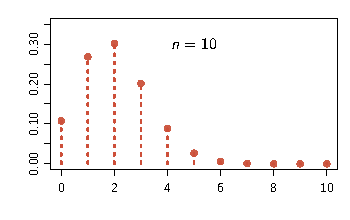
\includegraphics{Resources/Plots/BinomialVtlg1-1} 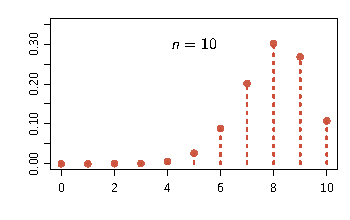
\includegraphics{Resources/Plots/BinomialVtlg1-2} 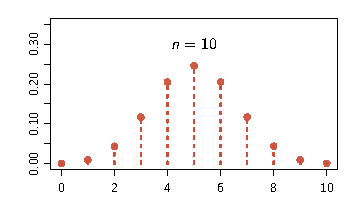
\includegraphics{Resources/Plots/BinomialVtlg1-3} \end{center}
\normalsize
\end{frame}

\begin{frame}{Binomialverteilung}
\phantomsection\label{binomialverteilung-7}
\framesubtitle{Wahrscheinlichkeitsfunktion}

\begin{itemize}
\tightlist
\item
  Den Effekt von \(n\) bei konstantem \(p\) verdeutlicht die folgende
  Abbildung.
\item
  In allen vier Fällen ist \(p=0.2\), die Anzahl der Durchführungen ist
  \(n=10\), \(n=30\), \(n=50\) und \(n=100\).
\item
  Die Symmetrie wird mit zunehmendem \(n\) ausgeprägter.
\end{itemize}
\end{frame}

\begin{frame}{Binomialverteilung}
\phantomsection\label{binomialverteilung-8}
\framesubtitle{Wahrscheinlichkeitsfunktion}

\footnotesize
\begin{center}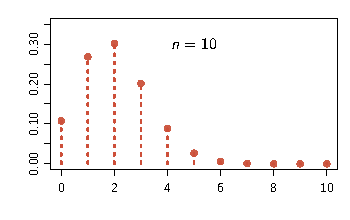
\includegraphics{Resources/Plots/BinomialVtlg2-1} 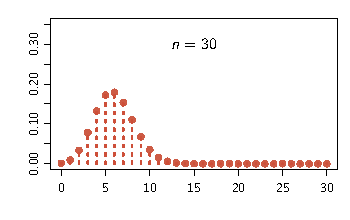
\includegraphics{Resources/Plots/BinomialVtlg2-2} 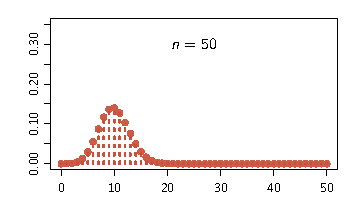
\includegraphics{Resources/Plots/BinomialVtlg2-3} 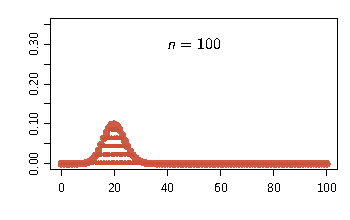
\includegraphics{Resources/Plots/BinomialVtlg2-4} \end{center}
\normalsize
\end{frame}

\begin{frame}{Binomialverteilung}
\phantomsection\label{binomialverteilung-9}
\framesubtitle{Verteilungsfunktion für $p=0.2$ und $n=10$}

\(F(x)\) macht bei \(x=2\), wo \(f(x)\) ein Maximum besitzt, den größten
Sprung.

\footnotesize
\begin{center}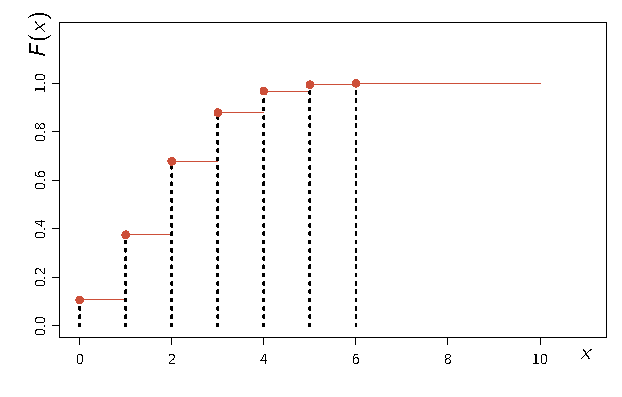
\includegraphics{Resources/Plots/BinomialVtlg3-1} \end{center}
\normalsize
\end{frame}

\begin{frame}{Binomialverteilung}
\phantomsection\label{binomialverteilung-10}
\framesubtitle{Erwartungswert und Varianz}
\vspace{1cm}

\begin{itemize}
\item
  Da \(X\) als \(X=\sum^n_{j=1} X_j\) definiert ist und jedes \(X_j\)
  einer Bernoulli-Verteilung mit dem Erwartungswert \(\E(X_j)=p\) folgt,
  gilt \begin{align}
  \mu=\E\left(\sum^n_{j=1}X_j\right)\stackrel{\eqref{EWSumme}}{=}\sum^n_{j=1} \E(X_j)=\sum\limits^n_{j=1}p=np. \label{EwertBinomial}
  \end{align}
\item
  Die Varianz von \(X\) lässt sich mit dem
  \hil{Additionssatz für Varianzen stochastisch unabhängiger Zufallsvariablen}
  \eqref{varSumme} ermitteln.
\item
  Da jedes \(X_j\), \(j=1,\ldots,n\) dieselbe Varianz \(\var(X_j)=pq\)
  besitzt, folgt für die Summe \(X\) \begin{align}
  \sigma^2= \var\left(\sum\limits^n_{j=1}X_j\right)=\sum\limits^n_{j=1}\var(X_j)=\sum\limits^n_{j=1}pq \stackrel{\eqref{BernouVar}}{=} n p q. \label{VarBinomial}
  \end{align}
\end{itemize}
\end{frame}

\begin{frame}{Binomialverteilung}
\phantomsection\label{binomialverteilung-11}
\framesubtitle{Varianz}

\begin{itemize}
\tightlist
\item
  Der Einfluss der \hil{Scharparameter} \(n\) und \(p\) kann an den
  Gleichungen \[\mu=np\qquad\text{ und }\qquad\sigma^2=npq\] erkannt
  werden.
\item
  Erhöht man \(n\) bei konstantem \(p\), steigen \(\mu\) und
  \(\sigma^2\); für die drei Verteilungen in der Abbildung erhält man
  \(\mu_1=2\), \(\sigma^2_1=1.6\), \(\mu_2=6\), \(\sigma^2_2=4.8\) und
  \(\mu_3=10\), \(\sigma^2_3=8\).
\item
  Eine größeres \(p\) bei konstantem \(n\) lässt \(\mu\) wachsen,
  während \(\sigma^2\) nur bis \(p=0.5\) steigt, dann wieder fällt.
\end{itemize}
\end{frame}

\begin{frame}{Binomialverteilung}
\phantomsection\label{binomialverteilung-12}
\framesubtitle{Beispiel - QuizAcademy}
\QuizAcademy{Verteilungen 1}\endQuizAcademy
\end{frame}

\begin{frame}{Binomialverteilung}
\phantomsection\label{binomialverteilung-13}
\framesubtitle{Beispiel}

\xmpl[Glücksrad]Bei einem Glücksspiel betrage die Wahrscheinlichkeit zu
gewinnen \(p=0.2\).\mps Die Binomialverteilung \(B(5,0.2)\) liefert die
Wahrscheinlichkeit, dass bei 5 Teilnahmen mindestens einmal gewonnen
wird, wenn die Spiele unabhängig sind. \(P(X\geq 1)\) berechnet sich
nach dem Additionssatz für disjunkte Ereignisse als \begin{align*}
P(X\geq1) & = f(x=1)+\ldots+f(x=5) \\
& = \binom{5}{1}\cdot 0.2\cdot 0.8^4 +\ldots+
\binom{5}{5}\cdot 0.2^5\cdot 0.8^0 \\
& = 0.4096+0.2048+0.0512+0.0064+0.0003=0.6723.
\end{align*} \endxmpl
\end{frame}

\begin{frame}[fragile]{Binomialverteilung}
\phantomsection\label{binomialverteilung-14}
\framesubtitle{Beispiel}

\xmpl[Glücksrad]
 Schneller findet man die gesuchte Wahrscheinlichkeit über das
Komplemantärereignis -- kein Gewinn --, das zu \(X=0\) führt. Aus
\[P(X=0)+P(X\geq1)=1\] folgt
\[P(X\geq1)=1-P(X=0)=1-\binom{5}{0}\cdot 0.2^0\cdot 0.8^5=1-0.3277=0.6723.\]
\(F(x)\) liefert die gesuchte Wahrscheinlichkeit \(P(X\leq x)\) direkt.
\endxmpl

\footnotesize

\begin{Shaded}
\begin{Highlighting}[]
\DecValTok{1} \SpecialCharTok{{-}} \FunctionTok{pbinom}\NormalTok{(}\AttributeTok{q =} \DecValTok{0}\NormalTok{, }\AttributeTok{size =} \DecValTok{5}\NormalTok{, }\AttributeTok{prob =} \FloatTok{0.2}\NormalTok{)}
\end{Highlighting}
\end{Shaded}

\begin{verbatim}
## [1] 0.6723
\end{verbatim}

\begin{Shaded}
\begin{Highlighting}[]
\FunctionTok{pbinom}\NormalTok{(}\AttributeTok{q =} \DecValTok{0}\NormalTok{, }\AttributeTok{size =} \DecValTok{5}\NormalTok{, }\AttributeTok{prob =} \FloatTok{0.2}\NormalTok{, }\AttributeTok{lower.tail =}\NormalTok{ F)}
\end{Highlighting}
\end{Shaded}

\begin{verbatim}
## [1] 0.6723
\end{verbatim}

\normalsize
\end{frame}

\begin{frame}[fragile]{Binomialverteilung}
\phantomsection\label{binomialverteilung-15}
\framesubtitle{in \R}

\footnotesize

\begin{Shaded}
\begin{Highlighting}[]
\NormalTok{x }\OtherTok{\textless{}{-}} \FunctionTok{rbinom}\NormalTok{(}\AttributeTok{n =} \DecValTok{10000}\NormalTok{, }\AttributeTok{size =} \DecValTok{5}\NormalTok{, }\AttributeTok{prob =} \FloatTok{0.2}\NormalTok{)}
\FunctionTok{head}\NormalTok{(x, }\AttributeTok{n =} \DecValTok{20}\NormalTok{)}
\end{Highlighting}
\end{Shaded}

\begin{verbatim}
##  [1] 2 3 1 0 1 1 1 1 0 1 2 2 1 1 2 1 0 0 0 0
\end{verbatim}

\begin{Shaded}
\begin{Highlighting}[]
\FunctionTok{mean}\NormalTok{(x) }\CommentTok{\# Stichprobenmittelwert}
\end{Highlighting}
\end{Shaded}

\begin{verbatim}
## [1] 1.007
\end{verbatim}

\begin{Shaded}
\begin{Highlighting}[]
\FunctionTok{var}\NormalTok{(x)  }\CommentTok{\# Stichprobenvarianz}
\end{Highlighting}
\end{Shaded}

\begin{verbatim}
## [1] 0.7963
\end{verbatim}

\begin{Shaded}
\begin{Highlighting}[]
\FunctionTok{dbinom}\NormalTok{(}\AttributeTok{x =} \DecValTok{0}\SpecialCharTok{:}\DecValTok{5}\NormalTok{, }\AttributeTok{size =} \DecValTok{5}\NormalTok{, }\AttributeTok{prob =} \FloatTok{0.2}\NormalTok{) }\CommentTok{\# Wahrscheinlichkeitsfunktion}
\end{Highlighting}
\end{Shaded}

\begin{verbatim}
## [1] 0.32768 0.40960 0.20480 0.05120 0.00640 0.00032
\end{verbatim}

\begin{Shaded}
\begin{Highlighting}[]
\FunctionTok{pbinom}\NormalTok{(}\AttributeTok{q =} \DecValTok{0}\SpecialCharTok{:}\DecValTok{5}\NormalTok{, }\AttributeTok{size =} \DecValTok{5}\NormalTok{, }\AttributeTok{prob =} \FloatTok{0.2}\NormalTok{) }\CommentTok{\# Verteilungsfunktion}
\end{Highlighting}
\end{Shaded}

\begin{verbatim}
## [1] 0.3277 0.7373 0.9421 0.9933 0.9997 1.0000
\end{verbatim}

\begin{Shaded}
\begin{Highlighting}[]
\FunctionTok{sum}\NormalTok{(x }\SpecialCharTok{==} \DecValTok{2}\NormalTok{) }\SpecialCharTok{/} \DecValTok{10000} \CommentTok{\# relative Häufigkeit der Realisationen gleich zwei}
\end{Highlighting}
\end{Shaded}

\begin{verbatim}
## [1] 0.2074
\end{verbatim}

\normalsize
\end{frame}

\begin{frame}[fragile]{Binomialverteilung}
\phantomsection\label{binomialverteilung-16}
\framesubtitle{Beispiel}

\xmpl[Produktion]Bei einer Fertigung seien 5\% der Produkte fehlerhaft.
Zur Qualitätsprüfung werden 5 Produkte entnommen. Gesucht sind die
Wahrscheinlichkeiten für genau ein bzw. genau zwei defekte Produkte.
\begin{align*}
P(X=1) = f(x=1)&= \binom{5}{1}\cdot 0.05^1\cdot (1-0.05)^{5-1}\\
& = \frac{5!}{1!(5-1)!}\cdot 0.05\cdot 0.95^4 =0.2036.\\
P(X=2) = f(x=2)&= \binom{5}{2}\cdot 0.05^2\cdot (1-0.05)^{5-2}=0.0214.
\end{align*}

\footnotesize

\begin{Shaded}
\begin{Highlighting}[]
\FunctionTok{dbinom}\NormalTok{(}\AttributeTok{x =} \DecValTok{1}\SpecialCharTok{:}\DecValTok{2}\NormalTok{, }\AttributeTok{size =} \DecValTok{5}\NormalTok{, }\AttributeTok{prob =} \FloatTok{0.05}\NormalTok{)}
\end{Highlighting}
\end{Shaded}

\begin{verbatim}
## [1] 0.20363 0.02143
\end{verbatim}

\normalsize

\endxmpl
\end{frame}

\begin{frame}{Binomialverteilung}
\phantomsection\label{binomialverteilung-17}
\framesubtitle{Reproduktivität}

\begin{itemize}
\tightlist
\item
  Die Summe \(\tilde{S}=X+Y\) zweier unabhängiger und binomialverteilter
  Zufallsvariablen \(X\) und \(Y\) mit demselben \(p\) ist ebenfalls
  binomialverteilt.
\item
  Aus \(X\): \(B(m,p)\) und \(Y\): \(B(n,p)\) folgt also \(\tilde{S}\):
  \(B(m+n,p)\) -- die Binomialverteilung ist \hil{reproduktiv}.
\item
  Denn: Da \(X\) die Summe von \(m\) unabhängigen, zweipunktverteilten
  Zufallsvariablen und \(Y\) die Summe von \(n\) unabhängigen,
  zweipunktverteilten Zufallsvariablen ist, ist \(\tilde{S}\) die Summe
  von \(m+n\) unabhängigen zweipunktverteilten Zufallsvariablen.
\item
  Die Wahrscheinlichkeitsfunktion \(f(s)\) für \(s=0,1,2,\ldots,m+n\)
  ist daher analog zu \(f(x)\) \[f(s)=\binom{m+n}{s} p^sq^{m+n-s},\]
  null sonst.
\end{itemize}
\end{frame}

\begin{frame}{Geometrische Verteilung}
\phantomsection\label{geometrische-verteilung}
\begin{itemize}
\tightlist
\item
  Die Binomialverteilung liefert die Wahrscheinlichkeit für \(x\)-mal
  \emph{Erfolg} in einer Bernoulli-Kette mit Länge \(n\).
\item
  Manchmal interessiert aber die Wahrscheinlichkeit, dass eine
  Bernoulli-Kette die Länge \(n\) erreicht, bevor zum ersten Mal
  \emph{Erfolg} eintritt.
\item
  \(X\) ist nun definiert als Anzahl der Fehlversuche bis zum ersten
  Erfolg.
\item
  Bei \(X=0\) tritt der Erfolg bereits bei der ersten Durchführung ein,
  bei \(X=x\) bei der \((x+1)\)-ten Wiederholung.
\end{itemize}
\end{frame}

\begin{frame}{Geometrische Verteilung}
\phantomsection\label{geometrische-verteilung-1}
\framesubtitle{Wahrscheinlichkeitsfunktion}

\begin{itemize}
\tightlist
\item
  Die Wahrscheinlichkeiten für diese Ereignisse liefert der
  Multiplikationssatz für unabhängige Ereignisse \eqref{gemWSUnabh}.
\item
  Ist die Erfolgswahrscheinlichkeit wieder \(p\) (und für
  \emph{Misserfolg} \(q=1-p\)), ergibt sich
  \[ P(X=0)=p,\; P(X=1)=pq,\; P(X=2)=pq^2, \text{ usw.} \]
\item
  Verallgemeinert erhält man die Wahrscheinlichkeitsfunktion \(f(x)\)
  als \begin{equation}
  f(x)=
  \begin{cases}
   pq^x & x=0,1,2,\ldots \label{DichteGeomVtlg}\\
   0 & \text{sonst}.\notag
  \end{cases}
  \end{equation}
\end{itemize}
\end{frame}

\begin{frame}{Geometrische Verteilung}
\phantomsection\label{geometrische-verteilung-2}
\framesubtitle{Verteilungsfunktion}
\vspace{1cm}

\begin{itemize}
\tightlist
\item
  Eine solche Zufallsvariable heißt \hil{geometrisch verteilt}; die
  Verteilung hängt nur von \(p\) ab. Kurzform: \(G(p)\).
\item
  Für \(f(x)\) gilt mit der Summenformel für eine geometrische Reihe
  \begin{eqnarray*}
   \sum\limits^\infty_{x=0}f(x)&=&p+pq+pq^2+\ldots \\
   &=&p(1+q+q^2+\ldots )\\
   &=& p\sum\limits^\infty_{x=0}q^x=p\frac{1}{1-q}=p\frac{1}{p}=1.
  \end{eqnarray*}
\item
  Für \(x=0,1,2,\ldots\) lautet die Verteilungsfunktion \vspace{-0.5em}
  \begin{equation*}
  F(x)=\sum\limits^x_{k=0}p q^k.
  \end{equation*}
\end{itemize}
\end{frame}

\begin{frame}{Geometrische Verteilung}
\phantomsection\label{geometrische-verteilung-3}
\framesubtitle{Verteilungsfunktion}

Das Buch auf S.~94-95 zeigt, dass \(F(x)\) geschrieben werden kann als
\begin{equation*}
  F(x)=
  \begin{cases}
   0& x<0 \\
   1-q^{[x]+1}& x\geq 0 \\
   1& x=\infty.
  \end{cases}
 \end{equation*} Beispiele für \(p=0.6\):

\footnotesize
\begin{center}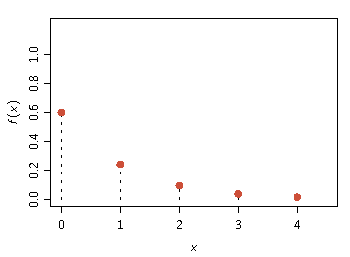
\includegraphics{Resources/Plots/GeometrischeVtlg1-1} 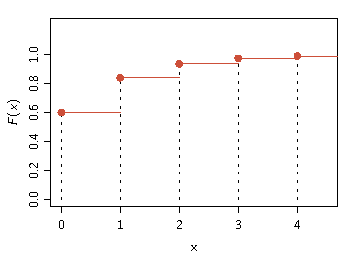
\includegraphics{Resources/Plots/GeometrischeVtlg1-2} \end{center}
\normalsize
\end{frame}

\begin{frame}{Geometrische Verteilung}
\phantomsection\label{geometrische-verteilung-4}
\framesubtitle{Verteilungsfunktion}

\begin{itemize}
\tightlist
\item
  Je größer \(p\), desto schneller strebt \(f(x)\) gegen null und
  \(F(x)\) gegen eins.
\item
  \(q^{x+1}\) ist die Komplementärwahrscheinlichkeit zu \(F(x)\).
\item
  Da \(F(x)=P(X\leq x)\), ist \(P(X>x)=q^{x+1}\).
\item
  Damit \(X>x\) überhaupt eintreten kann, müssen zunächst genau \(x+1\)
  Misserfolge vorliegen; die Anzahl nachfolgender Fehlversuche ist dann
  unerheblich.
\end{itemize}
\end{frame}

\begin{frame}{Geometrische Verteilung}
\phantomsection\label{geometrische-verteilung-5}
\framesubtitle{Wartezeitverteilung - Beispiel}

\xmpl[Investition]
 Bei einem Investitionsobjekt beträgt die Wahrscheinlichkeit, Gewinn pro
Periode zu erzielen: \(p=0.7\).\mps Wenn die Periodengewinne unabhängig
sind, liefert die geometrische Verteilung die Wahrscheinlichkeit für den
ersten Gewinn in der vierten Periode.\mps \(X\) nimmt den Wert \(x=3\)
an, \(F(x)\) ist an der Stelle \(x=3\) \[F(3)=1-0.3^4=0.9919.\]
\(F(3)=P(X\leq3)\) ist die Wahrscheinlichkeit dafür, dass es höchstens
drei Perioden dauert, bis in der vierten Periode der erste Gewinn
realisiert wird. Man bezeichnet \(G(p)\) wegen dieser Interpretation
auch als \hil{Wartezeitverteilung}. \endxmpl
\end{frame}

\begin{frame}{Geometrische Verteilung}
\phantomsection\label{geometrische-verteilung-6}
\framesubtitle{Wartezeitverteilung - Beispiel}

\xmpl[Investition]
 Die Wahrscheinlichkeit der geometrischen Verteilung
\(f(x=3)=0.7\cdot 0.3^3=0.0189\) darf nicht mit der Wahrscheinlichkeit
der Binomialverteilung verwechselt werden, die man für \(n=4\) und
\(x=1\) (Erfolg) erhält. Diese beträgt
\[f(x=1)=\binom{4}{1}0.7\cdot 0.3^3=0.0756.\] Sie gibt die
Wahrscheinlichkeit einer Bernoulli-Kette der Länge \(n=4\) mit einem
\emph{Erfolg} an. Da dieser nicht erst bei der vierten Durchführung
eintreten muss, ist die Wahrscheinlichkeit notwendigerweise größer als
bei der geometrischen Verteilung. \endxmpl
\end{frame}

\begin{frame}[fragile]{Geometrische Verteilung}
\phantomsection\label{geometrische-verteilung-7}
\framesubtitle{Wartezeitverteilung - Beispiel}

\xmpl[*]

\footnotesize

\begin{Shaded}
\begin{Highlighting}[]
\CommentTok{\# Verteilungsfunktion der geometrischen Verteilung}
\FunctionTok{pgeom}\NormalTok{(}\AttributeTok{q =} \DecValTok{3}\NormalTok{, }\AttributeTok{prob =} \FloatTok{0.7}\NormalTok{)}
\end{Highlighting}
\end{Shaded}

\begin{verbatim}
## [1] 0.9919
\end{verbatim}

\begin{Shaded}
\begin{Highlighting}[]
\CommentTok{\# Alternativ Berechnung über die Dichtefunktion}
\FunctionTok{sum}\NormalTok{(}\FunctionTok{dgeom}\NormalTok{(}\AttributeTok{x =} \DecValTok{0}\SpecialCharTok{:}\DecValTok{3}\NormalTok{, }\AttributeTok{prob =} \FloatTok{0.7}\NormalTok{))}
\end{Highlighting}
\end{Shaded}

\begin{verbatim}
## [1] 0.9919
\end{verbatim}

\begin{Shaded}
\begin{Highlighting}[]
\CommentTok{\# Zufallszahlen aus der Verteilung ziehen}
\FunctionTok{rgeom}\NormalTok{(}\AttributeTok{n =} \DecValTok{100}\NormalTok{, }\AttributeTok{prob =} \FloatTok{0.7}\NormalTok{)}
\end{Highlighting}
\end{Shaded}

\begin{verbatim}
##   [1] 0 0 0 0 0 0 0 0 1 0 0 1 1 0 0 0 0 0 1 0 1 1 1 0 0 0 0 4 1 0 0 0 0 1 1 0 0
##  [38] 0 1 2 0 2 0 0 1 2 0 0 0 0 2 0 0 0 0 2 0 0 0 0 0 0 0 0 0 0 0 1 0 2 1 0 0 0
##  [75] 0 1 1 0 0 0 2 0 0 2 0 0 1 0 0 0 0 0 0 0 0 2 0 0 0 0
\end{verbatim}

\begin{Shaded}
\begin{Highlighting}[]
\CommentTok{\# 3 tritt sehr selten auf, 4 so gut wie nie}
\end{Highlighting}
\end{Shaded}

\normalsize
\endxmpl
\end{frame}

\begin{frame}{Geometrische Verteilung}
\phantomsection\label{geometrische-verteilung-8}
\framesubtitle{Erwartungswert und Varianz}

Erwartungswert und Varianz der geometrischen Verteilung lauten
\[  \mu=\frac{q}{p} \] bzw. \[\sigma^2 = \frac{q}{p^2}.\] Eine
ausführliche Herleitung der beiden Parameter findet sich im Anhang.
\end{frame}

\begin{frame}{Geometrische Verteilung}
\phantomsection\label{geometrische-verteilung-9}
\framesubtitle{Erwartungswert und Varianz - QuizAcademy}
\QuizAcademy{Verteilungen 2}\endQuizAcademy
\end{frame}

\begin{frame}{Negative Binomialverteilung}
\phantomsection\label{negative-binomialverteilung}
\begin{itemize}
\tightlist
\item
  Die Problemstellung der geometrischen Verteilung lässt sich
  verallgemeinern: Wie oft ist ein Bernoulli-Experiment durchzuführen,
  bis genau \(r\) Erfolge eingetreten sind?
\item
  \(X\) ist jetzt definiert als die Anzahl der Misserfolge bis zum
  \(r\)-ten Erfolg.
\item
  Damit \(r\) Erfolge eintreten können, muss das Bernoulli-Experiment
  mindestens \(r\)-mal durchgeführt werden.
\item
  \(X=0\) bedeutet, dass alle \(r\) Durchführungen Erfolge sind; \(X=1\)
  bedeutet, dass sich der \(r\)-te Erfolg in der \((r+1)\)-ten
  Durchführung einstellt.
\item
  Allgemein bedeutet \(X=x\), dass der \(r\)-te Erfolg bei der
  \((x+r)\)-ten Ausführung vorliegt.
\item
  Bevor der \(r\)-te Erfolg eintritt, müssen in \(x+r-1\) Durchführungen
  genau \(r-1\) Erfolge realisiert worden sein; in der letzten, der
  \((x+r)\)-ten Wiederholung muss \emph{Erfolg} eintreten.
\end{itemize}
\end{frame}

\begin{frame}{Negative Binomialverteilung}
\phantomsection\label{negative-binomialverteilung-1}
\begin{itemize}
\item
  Die Wahrscheinlichkeit für \(r-1\) Erfolge bei \(x+r-1\)
  Durchführungen erhält man mit der Binomialverteilung
  \eqref{DichteBinomial} als \[ \binom{x+r-1}{r-1} p^{r-1}q^x. \]
\item
  Die Erfolgswahrscheinlichkeit im \((x+r)\)-ten Durchgang beträgt wie
  bei allen anderen Durchführungen \(p\).
\item
  Die Wahrscheinlichkeit, dass der \(r\)-te Erfolg genau bei der
  \((r+x)\)-ten Durchführung eintritt, ist wegen Unabhängigkeit der
  Experimente das Produkt beider Wahrscheinlichkeiten.
\item
  Damit lautet \begin{equation*}
  f(x)=
  \begin{cases}
   \dbinom{x+r-1}{r-1}p^rq^x& x=0,1,2,\ldots \\
   0& \text{sonst}.
  \end{cases}
   \end{equation*}
\end{itemize}
\end{frame}

\begin{frame}{Negative Binomialverteilung}
\phantomsection\label{negative-binomialverteilung-2}
\framesubtitle{Verteilungsfunktion}

\begin{itemize}
\tightlist
\item
  Eine solche Zufallsvariable heißt \hil{negativ binomialverteilt} oder
  auch \hil{Pascal-verteilt}.
\item
  Die negative Binomialverteilung hängt von den Parametern \(r\) und
  \(p\) ab; symbolisiere sie daher mit \(NB(r,p)\).
\item
  Die Verteilungsfunktion lautet \begin{equation*}
  F(x) =
  \begin{cases}
   0& x<0 \\
   \sum\limits_{k=0}^{[x]}\dbinom{k+r-1}{r-1}p^rq^k& 0\leq x,\quad k=0,1,\ldots[x].
  \end{cases}
   \end{equation*}
\end{itemize}
\end{frame}

\begin{frame}{Negative Binomialverteilung}
\phantomsection\label{negative-binomialverteilung-3}
\framesubtitle{Wahrscheinlichkeits- und Verteilungsfunktion}

In der Abbildung sind Wahrscheinlichkeits- und Verteilungsfunktion der
negativen Binomialverteilung für \(r=4\) und \(p=0.5\) dargestellt.

\footnotesize
\begin{center}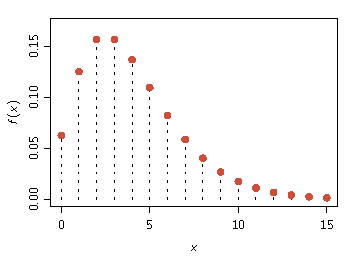
\includegraphics{Resources/Plots/NegBinomialVtlg1-1} 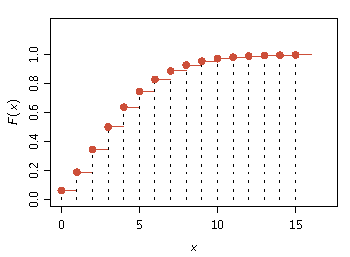
\includegraphics{Resources/Plots/NegBinomialVtlg1-2} \end{center}
\normalsize
\end{frame}

\begin{frame}{Negative Binomialverteilung}
\phantomsection\label{negative-binomialverteilung-4}
\framesubtitle{Erwartungswert und Varianz}

\begin{itemize}
\tightlist
\item
  Die Herleitung des Erwartungswertes und der Varianz finden sich im
  Buch auf S.~96-97.
\item
  Erwartungswert und Varianz für \(X\) betragen \begin{eqnarray*}
  \mu &=& %\E\left(\sum_{j=1}^r X_j \right) = \sum_{j=1}^r \E(X_j) =
  \frac{rq}{p} \quad \text{und} \\
  \sigma^2 &=& %\var\left(\sum_{j=1}^r X_j\right)  = \sum_{j=1}^r \var(X_j) =
  \frac{rq}{p^2}.
  \end{eqnarray*}
\end{itemize}
\end{frame}

\begin{frame}{Negative Binomialverteilung}
\phantomsection\label{negative-binomialverteilung-5}
\framesubtitle{Beispiel}

\xmpl[Glücksspiel]Bei einem Glücksspiel hat derjenige gewonnen, der
4-mal die 6 mit der geringsten Anzahl an Würfen erzielt. Die
Wahrscheinlichkeit, dass ein Teilnehmer dieses Ziel mit sechs Würfen
erreicht, lässt sich mit der negativen Binomialverteilung berechnen.\mps
In diesem Fall muss beim sechsten Wurf zum vierten Mal die 6 eintreten.
Die Parameter der negativen Binomialverteilung lauten \(p=\frac{1}{6}\)
und \(r=4\); \(X\) nimmt den Wert zwei an. Es ergibt sich
\[f(2)= \binom{5}{3}p^4q^2=0.0054.\] \endxmpl
\end{frame}

\begin{frame}{Negative Binomialverteilung}
\phantomsection\label{negative-binomialverteilung-6}
\framesubtitle{Beispiel}

\xmpl[*]Der Erwartungswert des Spiels beträgt dann
\[\mu = \frac{4\cdot5/6}{1/6}=20,\] d.h. der vierte Erfolg kann nach 20
Misserfolgen erwartet werden bzw. es muss bis zum vierten Erfolg
durchschnittlich 24-mal gespielt werden.\mps Die Varianz folgt als
\[\sigma^2=\frac{4\cdot 5/6}{1/36}=120,\] oder \(\sigma=10.9545\). Je
größer \(\sigma^2\), desto geringer ist die Information, die der
Erwartungswert, als mittlere Wartezeit interpretiert, liefert. \endxmpl
\end{frame}

\begin{frame}[fragile]{Negative Binomialverteilung}
\phantomsection\label{negative-binomialverteilung-7}
\framesubtitle{Beispiel}

\xmpl[*]

\footnotesize

\begin{Shaded}
\begin{Highlighting}[]
\FunctionTok{dnbinom}\NormalTok{(}\AttributeTok{x =} \DecValTok{2}\NormalTok{, }\AttributeTok{size =} \DecValTok{4}\NormalTok{, }\AttributeTok{prob =} \DecValTok{1}\SpecialCharTok{/}\DecValTok{6}\NormalTok{)}
\end{Highlighting}
\end{Shaded}

\begin{verbatim}
## [1] 0.005358
\end{verbatim}

\begin{Shaded}
\begin{Highlighting}[]
\FunctionTok{plot}\NormalTok{(}\AttributeTok{x =} \DecValTok{0}\SpecialCharTok{:}\DecValTok{60}\NormalTok{, }\AttributeTok{y =} \FunctionTok{dnbinom}\NormalTok{(}\AttributeTok{x =} \DecValTok{0}\SpecialCharTok{:}\DecValTok{60}\NormalTok{, }\AttributeTok{size =} \DecValTok{4}\NormalTok{, }\AttributeTok{prob =} \DecValTok{1}\SpecialCharTok{/}\DecValTok{6}\NormalTok{), }\AttributeTok{pch =} \DecValTok{19}\NormalTok{,}
     \AttributeTok{col =} \StringTok{"tomato3"}\NormalTok{, }\AttributeTok{ylab =} \StringTok{"$f(x)$"}\NormalTok{, }\AttributeTok{xlab =} \StringTok{"$x$"}\NormalTok{)}
\end{Highlighting}
\end{Shaded}

\begin{center}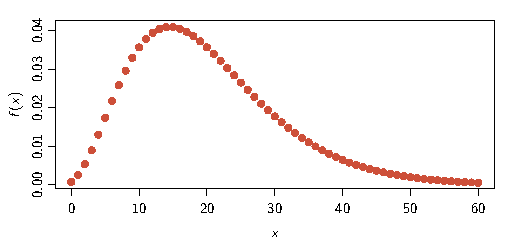
\includegraphics{Resources/Plots/unnamed-chunk-14-1} \end{center}
\normalsize
\endxmpl
\end{frame}

\begin{frame}{Hypergeometrische Verteilung}
\phantomsection\label{hypergeometrische-verteilung}
\begin{itemize}
\tightlist
\item
  Den bisher behandelten Verteilungen liegt \emph{Ziehen mit
  Zurücklegen} zugrunde.
\item
  Die \hil{hypergeometrische Verteilung} ergibt sich, wenn die
  Zufallsvorgänge durch \emph{Ziehen ohne Zurücklegen} charakterisiert
  werden können, bei denen wieder nur das Eintreten einer Eigenschaft
  \(A\) relevant ist.
\item
  Ausgangspunkt ist daher eine endliche Grundgesamtheit vom Umfang
  \(N\), bei der \(M<N\) Elemente eine Eigenschaft \(A\) besitzen, die
  übrigen \(N-M\) Elemente nicht.
\item
  Die Zufallsvariablen \(X_j\), \(j=1,\ldots,n\), sind eins, wenn das
  gezogene Element bei der \(j\)-ten Entnahme \(A\) aufweist; sie sind
  null wenn nicht.
\item
  Zieht man \(n\)-mal ohne Zurücklegen, gibt \(X=\sum^n_{j=1}X_j\) an,
  wie viele der Entnahmen die Eigenschaft \(A\) aufweisen.
\end{itemize}
\end{frame}

\begin{frame}{Hypergeometrische Verteilung}
\phantomsection\label{hypergeometrische-verteilung-1}
\framesubtitle{Wahrscheinlichkeits- und Verteilungsfunktion}

\begin{itemize}
\tightlist
\item
  Um Wahrscheinlichkeiten zu bestimmen, muss zunächst die Anzahl der
  Möglichkeiten, \(n\) Elemente aus \(N\) auszuwählen, berechnet werden.
\item
  Es gibt \(\binom{N}{n}\) Möglichkeiten, siehe \eqref{BinKoeff}.
\item
  Wir nehmen an, dass sie alle die gleiche Ziehungswahrscheinlichkeit
  besitzen.
\item
  Für \(P(X=x)\) benötigt man die Anzahl der Möglichkeiten, die \(x\)
  Elemente mit \(A\) enthalten.
\item
  Es gibt \(\binom{M}{x}\) Möglichkeiten, \(x\) aus \(M\) Elementen ohne
  Zurücklegen auszuwählen, siehe wiederum \eqref{BinKoeff}.
\end{itemize}
\end{frame}

\begin{frame}{Hypergeometrische Verteilung}
\phantomsection\label{hypergeometrische-verteilung-2}
\framesubtitle{Wahrscheinlichkeits- und Verteilungsfunktion}

\begin{itemize}
\tightlist
\item
  Zu jeder dieser Möglichkeiten existieren \(\binom{N-M}{n-x}\)
  Möglichkeiten, \(n-x\) Elemente aus \(N-M\) Elementen auszuwählen, die
  nicht \(A\) aufweisen.
\item
  Insgesamt gibt es somit \(\binom{M}{x}\binom{N-M}{n-x}\)
  Möglichkeiten, die \(x\) Elemente mit Eigenschaft \(A\) enthalten.
\item
  Das Verhältnis dieser Anzahl zu den insgesamt möglichen Auswahlen ist
  die Wahrscheinlichkeit für \(X=x\).
\end{itemize}
\end{frame}

\begin{frame}{Hypergeometrische Verteilung}
\phantomsection\label{hypergeometrische-verteilung-3}
\framesubtitle{Wahrscheinlichkeits- und Verteilungsfunktion}

\begin{itemize}
\tightlist
\item
  Die Wahrscheinlichkeitsfunktion resultiert also als
  \begin{eqnarray*}\notag
  & & f(x)=
  \begin{cases}
   \frac{\binom{M}{x}\binom{N-M}{n-x}}{\binom{N}{n}} & \max\{0,n+M-N\} \leq x \leq \min\{n,M\} \\ 0 &  \text{sonst}.
  \end{cases} \\
   \end{eqnarray*}
\item
  Die Verteilungsfunktion folgt hieraus durch Summation über \(k\):
  \begin{eqnarray*}\notag
  & & F(x)=
  \begin{cases}
   0 &  x<\max\{0,n+M-N\}=a \\
   \frac{\sum_{k=a}^{[x]}\binom{M}{k}\binom{N-M}{n-k}}{\binom{N}{n}} &  a \leq x \leq \min\{n,M\}, \quad k=a,\ldots, [x]\\
   1 & x>\min\{n,M\} \\
  \end{cases} \\
   \end{eqnarray*}
\item
  Die Beschränkungen für den Wertebereich von \(X\) werden im Buch auf
  S.~109 hergeleitet.
\end{itemize}
\end{frame}

\begin{frame}{Hypergeometrische Verteilung}
\phantomsection\label{hypergeometrische-verteilung-4}
\framesubtitle{Wahrscheinlichkeits- und Verteilungsfunktion}

\begin{itemize}
\tightlist
\item
  \(f(x)\) und \(F(x)\) zeigen, dass die hypergeometrische Verteilung
  die Parameter \(N,\) \(M\) und \(n\) besitzt; kürze sie daher mit
  \(H(N,M,n)\) ab.
\item
  In der folgenden Abbildung unterscheiden sich die \(f(x)\) nur in
  \(M\):
\end{itemize}

\footnotesize
\begin{center}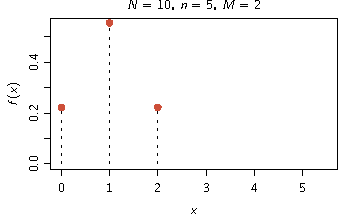
\includegraphics{Resources/Plots/HyperGeomVtlg1-1} 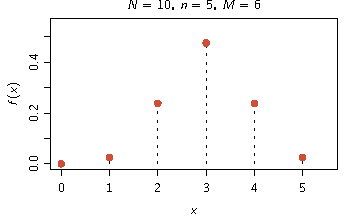
\includegraphics{Resources/Plots/HyperGeomVtlg1-2} \end{center}
\normalsize

\begin{itemize}
\tightlist
\item
  Mit zunehmendem \(M\) wandert \(f(x)\) nach rechts.
\end{itemize}
\end{frame}

\begin{frame}{Hypergeometrische Verteilung}
\phantomsection\label{hypergeometrische-verteilung-5}
\framesubtitle{Erwartungswert und Varianz}

\begin{itemize}
\tightlist
\item
  Erwartungswert und Varianz der hypergeometrischen Verteilung sind
  (Herleitung siehe Anhang):
  \[  \mu=np\quad\text{bzw.}\quad\sigma^2=np(1-p)\dfrac{N-n}{N-1}.\]
\item
  Binomial- und hypergeometrische Verteilung besitzen denselben
  Erwartungswert, obwohl sich die zugrunde liegenden Zufallsvorgänge
  unterscheiden (vgl. \eqref{EwertBinomial}).
\item
  Für den Erwartungswert ist es daher unbedeutend, ob bei dem
  Urnenmodell das entnommene Element zurückgelegt wird oder nicht.
\item
  Die \hil{Varianz} der hypergeometrischen Verteilung stimmt bis auf den
  Faktor \(\frac{N-n}{N-1}\) auch mit der für die Binomialverteilung
  überein (vgl. \eqref{VarBinomial}).
\end{itemize}
\end{frame}

\begin{frame}{Hypergeometrische Verteilung}
\phantomsection\label{hypergeometrische-verteilung-6}
\framesubtitle{Korrekturfaktor}

\begin{itemize}
\tightlist
\item
  Da sich beim \emph{Ziehen mit Zurücklegen} die Grundgesamtheit nicht
  erschöpft, nennt man \(\frac{N-n}{N-1}\) den
  \hil{Korrekturfaktor für endliche Gesamtheiten}.
\item
  Bei \(N=n\) ist, logischerweise, \(\sigma^2=0\) (warum?).
\item
  Für hinreichend große \(N\) gilt
  \[\frac{N-n}{N-1}\approx \frac{N-n}{N}=1-\frac{n}{N}.\]
\item
  Der Korrekturfaktor ist bei kleinem Auswahlsatz \(n/N\) fast eins.
\item
  Dann bleibt die Wahrscheinlichkeit, Elemente mit \(A\) zu erhalten,
  auch beim \emph{Ziehen ohne Zurücklegen} von Entnahme zu Entnahme fast
  gleich.
\item
  Die Binomialverteilung kann als Approximation für die
  hypergeometrische Verteilung dienen, wenn der \hil{Auswahlsatz}
  \(n/N\) kleiner als 5\% ist.
\end{itemize}
\end{frame}

\begin{frame}[fragile]{Hypergeometrische Verteilung}
\phantomsection\label{hypergeometrische-verteilung-7}
\framesubtitle{Vergleich Binomial- und hypergeometrische Verteilung}

\footnotesize

\begin{Shaded}
\begin{Highlighting}[]
\NormalTok{N }\OtherTok{\textless{}{-}} \DecValTok{200}\NormalTok{; n }\OtherTok{\textless{}{-}} \DecValTok{5}
\NormalTok{x }\OtherTok{\textless{}{-}} \DecValTok{0}\SpecialCharTok{:}\NormalTok{N; M }\OtherTok{\textless{}{-}} \DecValTok{80}
\NormalTok{p }\OtherTok{\textless{}{-}}\NormalTok{ M}\SpecialCharTok{/}\NormalTok{N}

\FunctionTok{plot}\NormalTok{(x, }\FunctionTok{dbinom}\NormalTok{(x,n,p), }\AttributeTok{xlim =} \FunctionTok{c}\NormalTok{(}\DecValTok{0}\NormalTok{,n), }\AttributeTok{cex =} \FloatTok{1.3}\NormalTok{, }\AttributeTok{col =} \StringTok{"blue"}\NormalTok{, }\AttributeTok{lwd =} \DecValTok{2}\NormalTok{, }\AttributeTok{ylab =} \StringTok{"Dichte"}\NormalTok{)}
\end{Highlighting}
\end{Shaded}

\normalsize

\footnotesize
\begin{center}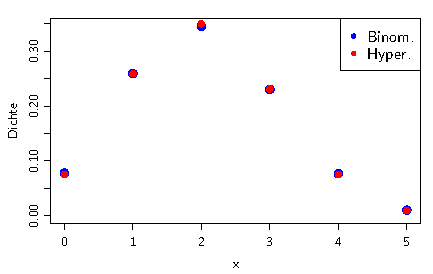
\includegraphics{Resources/Plots/HyperGeoAnhang2-1} \end{center}
\normalsize
\end{frame}

\begin{frame}{Hypergeometrische Verteilung}
\phantomsection\label{hypergeometrische-verteilung-8}
\framesubtitle{Beispiel}

\xmpl[Lotto, 6 aus 49 (bis 2013)]
 Man kann sechs der Zahlen 1 bis 49 auf
\(\binom{N}{n}=\binom{49}{6}=13\,983\, 816\) unterschiedliche Arten
ankreuzen. Durch Ziehen ohne Zurücklegen werden sechs Gewinnzahlen
ermittelt.\mps Damit sind die 49 Zahlen in eine Teilmenge mit den
\(M=6\) Gewinnzahlen und eine andere Teilmenge der \(N-M=43\) restlichen
Zahlen aufgeteilt.\mps Die Wahrscheinlichkeit, dass in einer Kombination
\(x=0,1,2,\ldots,6\) Gewinnzahlen vorkommen, erhält man aus
\[f(x)=\dfrac{\binom{6}{x}\binom{43}{6-x}}{\binom{49}{6}}.\] \endxmpl
\end{frame}

\begin{frame}{Hypergeometrische Verteilung}
\phantomsection\label{hypergeometrische-verteilung-9}
\framesubtitle{Beispiel}

\xmpl[*]Die Wahrscheinlichkeiten für \(x=0, x=3\) und \(x=5\) betragen
gerundet
\[ f(x=0)=0.4360,\; f(x=3)=0.0177 \text{ und } f(x=5)=0.00002.\] Nach
der Ziehung der sechs Gewinnzahlen wird eine Zusatzzahl gezogen. Die
Wahrscheinlichkeit für das Ereignis \emph{drei Gewinnzahlen (GZ) und die
Zusatzzahl (ZZ)} erhalten wir aus \begin{eqnarray*}
P(\text{GZ}=x\text{ und ZZ})&=&P(\text{ZZ}|\text{GZ}=x)P(\text{GZ}=x)\\
&=&\frac{6-x}{43}f(x).
\end{eqnarray*} \endxmpl
\end{frame}

\begin{frame}[fragile]{Hypergeometrische Verteilung}
\phantomsection\label{hypergeometrische-verteilung-10}
\framesubtitle{Beispiel}
\xmpl[*]

\footnotesize

\begin{Shaded}
\begin{Highlighting}[]
\CommentTok{\# WSK für 0, 1, 2, ..., 6 Gewinnzahlen}
\FunctionTok{round}\NormalTok{(}\FunctionTok{dhyper}\NormalTok{(}\AttributeTok{x =} \DecValTok{0}\SpecialCharTok{:}\DecValTok{6}\NormalTok{, }\AttributeTok{m =} \DecValTok{6}\NormalTok{, }\AttributeTok{n =} \DecValTok{43}\NormalTok{, }\AttributeTok{k =} \DecValTok{6}\NormalTok{), }\DecValTok{5}\NormalTok{)}
\end{Highlighting}
\end{Shaded}

\begin{verbatim}
## [1] 0.43596 0.41302 0.13238 0.01765 0.00097 0.00002 0.00000
\end{verbatim}

\begin{Shaded}
\begin{Highlighting}[]
\CommentTok{\# 3 Gewinnzahlen + Zusatzzahl}
\CommentTok{\# m = 6 {-}\textgreater{} 6 mögliche Treffer, m = 3 {-}\textgreater{} nur noch 3 mögliche Treffer}
\FunctionTok{dhyper}\NormalTok{(}\AttributeTok{x =} \DecValTok{3}\NormalTok{, }\AttributeTok{m =} \DecValTok{6}\NormalTok{, }\AttributeTok{n =} \DecValTok{43}\NormalTok{, }\AttributeTok{k =} \DecValTok{6}\NormalTok{) }\SpecialCharTok{*} \FunctionTok{dhyper}\NormalTok{(}\AttributeTok{x =} \DecValTok{1}\NormalTok{, }\AttributeTok{m =} \DecValTok{3}\NormalTok{, }\AttributeTok{n =} \DecValTok{40}\NormalTok{, }\AttributeTok{k =} \DecValTok{1}\NormalTok{)}
\end{Highlighting}
\end{Shaded}

\begin{verbatim}
## [1] 0.001231
\end{verbatim}

\normalsize
\mps

Man bemerke (siehe \texttt{?dhyper}), dass \(\texttt{m}=M\),
\(\texttt{n}=N-M\) und \(\texttt{k}=n\).

Beachte außerdem im letzten Schritt, dass \(M=6-x\), \(x=1\), \(n=1\)
und \(N=43\), so dass \[
\frac{{6-x \choose 1}{43-(6-x) \choose 0}}{{43 \choose 1}}=\frac{6-x}{43}
\] \endxmpl
\end{frame}

\begin{frame}{Ausgewählte diskrete Verteilungen}
\phantomsection\label{ausgewuxe4hlte-diskrete-verteilungen}
\framesubtitle{Aufgaben}
\exe

Geben Sie für \(X\), das aus dem Zufallsexperiment \emph{einmaliger
Würfelwurf} resultiert, die Wahrscheinlichkeits- und die
Verteilungsfunktion an! \endexe \exe Aus einer Urne mit zwei weißen
Kugeln und einer schwarzen Kugel wird einmal gezogen. \(X\) nimmt 1 an,
wenn \emph{weiß} gezogen wird und 0, wenn \emph{schwarz} gezogen wird.
Geben Sie für \(X\) die Wahrscheinlichkeits- und die Verteilungsfunktion
an! \endexe
\end{frame}

\begin{frame}{Ausgewählte diskrete Verteilungen}
\phantomsection\label{ausgewuxe4hlte-diskrete-verteilungen-1}
\framesubtitle{Aufgaben}
\exe

In einer Urne befinden sich 30 grüne und 60 schwarze Kugeln. Es werden 4
Kugeln mit Zurücklegen aus der Urne entnommen.

\begin{enumerate}
[(a)]
\tightlist
\item
  Wie groß ist die Wahrscheinlichkeit 2 grüne Kugeln zu ziehen?
\item
  Wie groß ist die Wahrscheinlichkeit höchstens 2 grüne Kugeln zu
  ziehen?
\item
  Berechnen Sie den Erwartungswert und die Varianz für \(X\)!
\end{enumerate}

\endexe
\end{frame}

\begin{frame}{Ausgewählte diskrete Verteilungen}
\phantomsection\label{ausgewuxe4hlte-diskrete-verteilungen-2}
\framesubtitle{Aufgaben}
\exe

In einer Urne befinden sich 10 Kugeln von denen 6 schwarz und die
restlichen weiß sind. Wenn 5 Kugeln aus der Urne ohne Zurücklegen
gezogen werden, wie groß ist die Wahrscheinlichkeit, dass 3 davon
schwarz sind? \endexe \exe Zufallsexperiment: Einmaliger Würfelwurf.

\begin{enumerate}
[(a)]
\tightlist
\item
  Wie groß ist die Wahrscheinlichkeit, dass im 8. Wurf das 3. Mal die 6
  gefallen ist?
\item
  Wie groß ist die Wahrscheinlichkeit, dass spätestens im 8. Wurf die
  dritte 6 fällt?
\item
  Wie oft muss durchschnittlich gewürfelt werden bis die dritte 6 fällt?
\end{enumerate}

\endexe
\end{frame}

\begin{frame}{Ausgewählte diskrete Verteilungen}
\phantomsection\label{ausgewuxe4hlte-diskrete-verteilungen-3}
\framesubtitle{Aufgaben}
\exe

Bei der Untersuchung von Investitionstätigkeiten von Bankangestellten
hat sich herausgestellt, dass pro Jahr 15 Transaktionen an der Börse
getätigt werden.

\begin{enumerate}
[(a)]
\tightlist
\item
  Wie groß ist die Wahrscheinlichkeit, dass in einem Jahr eine
  Transaktion durchgeführt wird?
\item
  Wie groß ist die Wahrscheinlichkeit, dass in einem Monat eine
  Transaktion durchgeführt wird?
\end{enumerate}

\endexe

\exe

Ein Basketballspieler hat während seiner Karriere 84\% seiner Freiwürfe
verwandelt. Wie groß ist die Wahrscheinlichkeit, dass er in einem Spiel
6 von 16 Freiwürfen nicht verwandelt? \endexe
\end{frame}

\begin{frame}{Ausgewählte diskrete Verteilungen}
\phantomsection\label{ausgewuxe4hlte-diskrete-verteilungen-4}
\framesubtitle{Aufgaben}
\vspace{1cm}
\exe

In einer Gruppe von 10 Personen präferieren 6 Personen Cola und die
restlichen Personen Fanta. Wenn 3 Personen aus dieser Gruppe nach ihrem
Lieblingsgetränk gefragt werden, wie groß ist die Wahrscheinlichkeit,
dass die Mehrheit Fanta bevorzugt? \endexe \exe Ein Student kommt nach
einer Studentenparty angetrunken nach Hause. Er hat einen Schlüsselbund
mit 8 Schlüsseln und sucht nach dem Haustürschlüssel.

\begin{enumerate}
[(a)]
\tightlist
\item
  Wie groß ist die Wahrscheinlichkeit, dass der 6. Schlüssel, den er
  ausprobiert in das Schloss passt?
\item
  Wie groß ist die Wahrscheinlichkeit, dass spätestens der 6. Schlüssel
  passt?
\item
  Wie viele Schlüssel muss er durchschnittlich ausprobieren bis er den
  richtigen Schlüssel gefunden hat?
\end{enumerate}

\endexe
\end{frame}

\begin{frame}{Ausgewählte diskrete Verteilungen}
\phantomsection\label{ausgewuxe4hlte-diskrete-verteilungen-5}
\framesubtitle{Aufgaben}
\exe

Ein Spieler setzt beim Roulettespiel bei jedem der 200 durchgeführten
Spiele auf die 17. Die Wahrscheinlichkeit einmal zu gewinnen ist
\(P(\text{Zahl}\; 17)=\frac{1}{37}=0.027\).\mps Wie groß ist die
Wahrscheinlichkeit, dass er genau acht Mal gewinnt? \endexe
\end{frame}

\begin{frame}{Normalverteilung}
\phantomsection\label{normalverteilung}
\begin{itemize}
\tightlist
\item
  Die wohl wichtigste Verteilung der Statistik ist die
  \hil{Normalverteilung}. Sie wurde von de Moivre, Laplace und Gauß
  entwickelt.
\item
  Die Normalverteilung beschreibt bestimmte konkrete empirische
  Verteilungen recht gut.
\item
  Für die Induktive Statistik aber noch bedeutsamer ist, dass bei
  hinreichend großem Stichprobenumfang auch viele in der Schätz- und
  Testtheorie auftretenden theoretischen Verteilungen durch die
  Normalverteilung gut approximiert werden.
\end{itemize}
\end{frame}

\begin{frame}{Normalverteilung}
\phantomsection\label{normalverteilung-1}
\framesubtitle{Dichte- und Verteilungsfunktion}

\begin{itemize}
\item
  Die Dichte der Normalverteilung lautet
  \[f(x) \stackrel{\text{Def.} \, \ref{DichteFkt}}{=}\frac{1}{\sqrt{2\pi}\sigma}\text{e}^{-\frac{1}{2}\left(\frac{x-\mu}{\sigma}\right)^2} \; , \quad -\infty < x < \infty, \]
  mit Erwartungswert \(\mu\) und Varianz \(\sigma^2\) als
  Scharparameter.
\item
  Daraus erhält man die Verteilungsfunktion als \begin{equation*}
  F(x) \stackrel{\text{Def.} \, \ref{VtlgFunktion}}{=}\frac{1}{\sqrt{2\pi}\sigma}\int\limits_{-\infty}^x  \text{e}^{-\frac{1}{2}\left(\frac{u-\mu}{\sigma}\right)^2} \, du  \; , \quad -\infty < x < \infty.
  \end{equation*}
\item
  Die Normalverteilung wird abgekürzt mit \(N(\mu,\sigma^2)\).
\end{itemize}
\end{frame}

\begin{frame}{Normalverteilung}
\phantomsection\label{normalverteilung-2}
\framesubtitle{Dichte- und Verteilungsfunktion für $\mu=0$ und $\sigma^2=1$}

\footnotesize
\begin{center}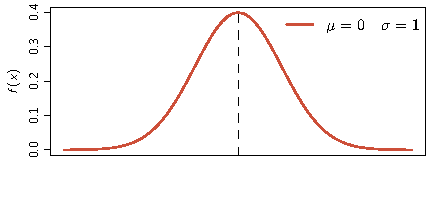
\includegraphics{Resources/Plots/NormalVtlg1-1} 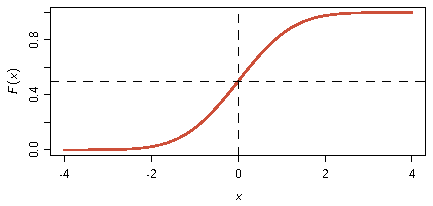
\includegraphics{Resources/Plots/NormalVtlg1-2} \end{center}
\normalsize
\end{frame}

\begin{frame}{Normalverteilung}
\phantomsection\label{normalverteilung-3}
\framesubtitle{Dichte- und Verteilungsfunktion}
\exe

Zeigen Sie, dass die Dichtefunktion der Normalverteilung an der Stelle
\(x=\mu\) ein Maximum besitzt! \endexe

\begin{itemize}
\tightlist
\item
  Die Dichtefunktion ist symmetrisch um \(\mu\); an den Stellen
  \(\mu+x\) und \(\mu-x\) nimmt \(f(x)\) für alle \(x\in\mathbb{R}\)
  dieselben Werte an.
\item
  Die Dichtefunktion fällt rechts und links von \(\mu\) streng monoton
  und nähert sich asymptotisch der Abszisse für
  \(x\rightarrow\pm\infty\).
\item
  Wegen der \hil{Symmetrie} gilt Median = Modus = Erwartungswert.
\item
  Also hat die Verteilungsfunktion bei \(x=\mu\) einen Wendepunkt.
\end{itemize}
\end{frame}

\begin{frame}{Normalverteilung}
\phantomsection\label{normalverteilung-4}
\framesubtitle{Variation von $\mu$ und $\sigma$}

\begin{itemize}
\tightlist
\item
  Wird \(\mu\) variiert, verschiebt sich die Dichtefunktion auf der
  \(x\)-Achse, ohne dass sich ihre Form ändert.
\item
  Die Auswirkung einer Variation von \(\sigma\) illustriert der
  Funktionswert \(f(x)\) an der Stelle \(x=\mu\):
  \[f(\mu)=\frac{1}{\sigma\sqrt{2\pi}}.\]
\item
  Nimmt \(\sigma\) zu, wird \(f(\mu)\) kleiner. Daher verläuft die
  Dichtefunktion mit zunehmendem \(\sigma\) flacher.
\item
  Die nächsten Abbildungen zeigen \(f(x)\)

  \begin{enumerate}
  [(a)]
  \tightlist
  \item
    für \(\mu=3\) und \(\mu=4\) bei konstantem \(\sigma\), sowie
  \item
    für \(\sigma^2=0.25\), \(\sigma^2=1\) und \(\sigma^2=4\) bei
    konstantem \(\mu=0\).
  \end{enumerate}
\end{itemize}
\end{frame}

\begin{frame}{Normalverteilung}
\phantomsection\label{normalverteilung-5}
\framesubtitle{Variation von $\mu$ und $\sigma$}

\footnotesize
\begin{center}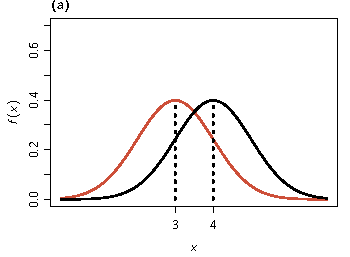
\includegraphics{Resources/Plots/NormalVtlg2-1} 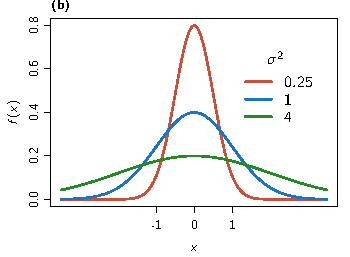
\includegraphics{Resources/Plots/NormalVtlg2-2} \end{center}
\normalsize
\end{frame}

\begin{frame}{Normalverteilung}
\phantomsection\label{normalverteilung-6}
\framesubtitle{Reproduktivitätseigenschaft}

\begin{itemize}
\tightlist
\item
  Die Normalverteilung besitzt die \hil{Reproduktivitätseigenschaft},
  d.h.~Linearkombinationen von normalverteilten \(X_1,\ldots,X_n\) sind
  auch normalverteilt.
\item
  Zwei wichtige Spezialfälle:

  \begin{enumerate}
  [(a)]
  \tightlist
  \item
    Die \hil{Summe} \(\tilde{S}\) der \(X_j\),
    \(\tilde{S}=\sum^n_{j=1}X_j\) und
  \item
    das \hil{arithmetische Mittel}
    \(\bar{X}=\frac{1}{n}\sum^n_{j=1}X_j\) sind normalverteilt.
  \end{enumerate}
\item
  Im folgenden Kapitel mehr zu den dann resultierenden Parametern der
  Normalverteilung von \(\tilde{S}\) und \(\bar{X}\).
\end{itemize}
\end{frame}

\begin{frame}{Normalverteilung}
\phantomsection\label{normalverteilung-7}
\framesubtitle{Lineartransformation}

\begin{itemize}
\tightlist
\item
  Ist \(X:N(\mu_X, \sigma^2_X)\), dann ist auch \(Y=a+bX\)
  normalverteilt mit Parametern
  \[\mu_Y\stackrel{\eqref{EWlinTrafo}}{=}a+b\mu_X\quad\text{und}\quad \sigma^2_Y\stackrel{\eqref{VarLinKomb3}}{=}b^2\sigma^2_X.\]
\item
  Die Transformation \begin{equation}\label{stdNormalTrafo}
  Y=a+b X\quad\text{mit}\quad a=-\mu_X/\sigma_X\quad\text{und}\quad b=1/\sigma_X
  \end{equation} führt zu einer standardisierten Zufallsvariablen
  (s.~\eqref{stdRV}), mit \(\mu_Y=0\) und \(\sigma^2_Y=1\).
\item
  Ist \(X\) normalverteilt, so ist die standardisierte Zufallsvariable
  \(Z\) \(N(0,1)\)-verteilt, d.h.~\hil{standardnormalverteilt}.
\item
  Zusammengefasst:
  \[  Z=\dfrac{X-\mu}{\sigma}, \text{ mit } X:\; N(\mu,\sigma^2) \text{ und }  Z:\; N(0,1).\]
\end{itemize}
\end{frame}

\begin{frame}{Standardnormalverteilung}
\phantomsection\label{standardnormalverteilung}
\framesubtitle{Dichte- und Verteilungsfunktion}

\begin{itemize}
\tightlist
\item
  Für die Wahrscheinlichkeiten gilt somit \begin{align}
   P(X\leq a) = P\left(Z\leq \dfrac{a-\mu}{\sigma}\right). \label{StdNormVtlgWsk}
   \end{align}
\item
  Dichte- und Verteilungsfunktion von \(Z\):
  \[f(z)= \frac{1}{\sqrt{2\pi}}\text{e}^{-\frac{z^2}{2}},\quad F(z)=\frac{1}{\sqrt{2\pi}}\int\limits_{-\infty}^z \text{e}^{-\frac{u^2}{2}}\; du.
  \]
\item
  Die Dichtefunktion hat das Maximum an der Stelle \(z=\mu=0\) und
  Wendepunkte bei \(z=\pm\sigma=\pm 1\); der Wendepunkt der
  Verteilungsfunktion \(F(z)\) liegt bei \(z=\mu=0\).
\end{itemize}
\end{frame}

\begin{frame}{Standardnormalverteilung}
\phantomsection\label{standardnormalverteilung-1}
\framesubtitle{Dichte- und Verteilungsfunktion}

\begin{itemize}
\tightlist
\item
  Die folgenden Graphen zeigen Dichte- und Verteilungsfunktion einer
  standardnormalverteilten Zufallsvariable:
\end{itemize}

\footnotesize
\begin{center}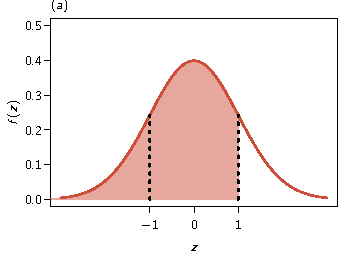
\includegraphics{Resources/Plots/StdNormalVtlg1-1} 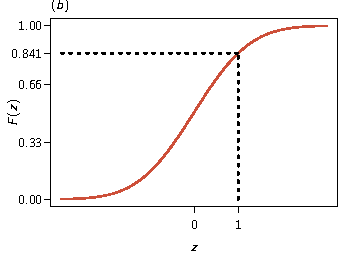
\includegraphics{Resources/Plots/StdNormalVtlg1-2} \end{center}
\normalsize
\end{frame}

\begin{frame}{Standardnormalverteilung}
\phantomsection\label{standardnormalverteilung-2}
\framesubtitle{Dichte- und Verteilungsfunktion - QuizAcademy}
\QuizAcademy{Verteilungen 3}\endQuizAcademy
\end{frame}

\begin{frame}{Standardnormalverteilung}
\phantomsection\label{standardnormalverteilung-3}
\framesubtitle{Dichte- und Verteilungsfunktion}

\begin{itemize}
\tightlist
\item
  \hil{Symmetrie} der Normalverteilung um Null impliziert, dass
  \[P(Z\leq -z_1)=P(Z\geq z_1)=1- P(Z\leq z_1)\] für jedes
  \(z_1 \in\mathbb{R}\).
\item
  Die rötliche Fläche in \blue{(a)} hat dieselbe Größe wie die Ordinate
  \(F(z_1)\) in (b): \(P(Z\leq z_1)\).
\item
  Die Wahrscheinlichkeit, dass \(Z\) Werte im Intervall \([z_1,z_2]\)
  annimmt, berechnet sich (wie üblich) als
  \[P(z_1\leq Z\leq z_2) = P(Z\leq z_2)-P(Z<z_1)=F(z_2)-F(z_1).\]
\end{itemize}
\end{frame}

\begin{frame}{Standardnormalverteilung}
\phantomsection\label{standardnormalverteilung-4}
\framesubtitle{Tabellierung der Verteilungsfunktion}

\begin{itemize}
\tightlist
\item
  Früher hat man \(F(z)\) in folgender Tabelle abgelesen:
  \vspace{-0.25em}

  \begin{scriptsize}
  \setlength{\tabcolsep}{.5mm}
  \begin{center}
  \begin{tabular}{|c|c|c|c|c|c|c|c|c|c|c|c}\cline{1-11}
  {\boldmath{$z$}} & {\bf 0.00}   & {\bf 0.01}   & {\bf 0.02}   & {\bf 0.03}   & {\bf 0.04}
  & {\bf 0.05} & {\bf 0.06} & {\bf 0.07} & {\bf 0.08} & {\bf 0.09} \\ \cline{1-11}
  {\bf 0.0} & 0.5000 & 0.5040 & 0.5080 & 0.5120 & 0.5160  &   0.5199  &   0.5239  &   0.5279  & 0.5319  &   0.5359 \\
  {\bf 0.1} &   0.5398  &   0.5438  &   0.5478  &   0.5517  & 0.5557  &   0.5596  &   0.5636  &   0.5675  & 0.5714  &   0.5753 \\
  {\bf 0.2} &   0.5793  &   0.5832  &   0.5871  &   0.5910  & 0.5948  &   0.5987  &   0.6026  &   0.6064  & 0.6103  &   0.6141 \\
  {\bf 0.3} &   0.6179  &   0.6217  &   0.6255  &   0.6293  & 0.6331  &   0.6368  &   0.6406  &   0.6443  & 0.6480  &   0.6517 \\
  {\bf 0.4} &   0.6554  &   0.6591  &   0.6628  &   0.6664  & 0.6700  &   0.6736  &   0.6772  &   0.6808  & 0.6844  &   0.6879 \\
  {\bf 0.5} &   0.6915  &   0.6950  &   0.6985  &   0.7019  & 0.7054  &   0.7088  &   0.7123  &   0.7157  & 0.7190  &   0.7224 \\
  {\bf 0.6} &   0.7257  &   0.7291  &   0.7324  &   0.7357  & 0.7389  &   0.7422  &   0.7454  &   0.7486  & 0.7517  &   0.7549 \\
  {\bf 0.7} &   0.7580  &   0.7611  &   0.7642  &   0.7673  & 0.7704  &   0.7734  &   0.7764  &   0.7794  & 0.7823  &   0.7852 \\
  {\bf 0.8} &   0.7881  &   0.7910  &   0.7939  &   0.7967  & 0.7995  &   0.8023  &   0.8051  &   0.8078  & 0.8106  &   0.8133 \\
  {\bf 0.9} &   0.8159  &   0.8186  &   0.8212  &   0.8238  & 0.8264  &   0.8289  &   0.8315  &   0.8340  & 0.8365  &   0.8389 \\
  {\bf 1.0} &   0.8413  &   0.8438  &   0.8461  &   0.8485  & 0.8508  &   0.8531  &   0.8554  &   0.8577  & 0.8599  &   0.8621 \\ \cline{1-11}
  {\bf 1.1} &   0.8643  &   0.8665  &   0.8686  &   0.8708  & 0.8729  &   0.8749  &   0.8770  &   0.8790  & 0.8810  &   0.8830 \\
  {\bf 1.2} &   0.8849  &   0.8869  &   0.8888  &   0.8907  & 0.8925  &   0.8944  &   0.8962  &   0.8980  & 0.8997  &   0.9015 \\
  {\bf 1.3} &   0.9032  &   0.9049  &   0.9066  &   0.9082  & 0.9099  &   0.9115  &   0.9131  &   0.9147  & 0.9162  &   0.9177 \\
  {\bf 1.4} &   0.9192  &   0.9207  &   0.9222  &   0.9236  & 0.9251  &   0.9265  &   0.9279  &   0.9292  & 0.9306  &   0.9319 \\
  {\bf 1.5} &   0.9332  &   0.9345  &   0.9357  &   0.9370  & 0.9382  &   0.9394  &   0.9406  &   0.9418  & 0.9429  &   0.9441 \\
  {\bf 1.6} &   0.9452  &   0.9463  &   0.9474  &   0.9484  & 0.9495  &   0.9505  &   0.9515  &   0.9525  & 0.9535  &   0.9545 \\
  {\bf 1.7} &   0.9554  &   0.9564  &   0.9573  &   0.9582  & 0.9591  &   0.9599  &   0.9608  &   0.9616  & 0.9625  &   0.9633 \\
  {\bf 1.8} &   0.9641  &   0.9649  &   0.9656  &   0.9664  & 0.9671  &   0.9678  &   0.9686  &   0.9693  & 0.9699  &   0.9706 \\
  {\bf 1.9} &   0.9713  &   0.9719  &   0.9726  &   0.9732  & 0.9738  &   0.9744  &   0.9750  &   0.9756  & 0.9761  &   0.9767 \\
  {\bf 2.0} &   0.9772  &   0.9778  &   0.9783  &   0.9788  & 0.9793  &   0.9798  &   0.9803  &   0.9808  & 0.9812  &   0.9817 \\ \cline{1-11}
  \end{tabular}
  \end{center}
  \end{scriptsize}
\end{itemize}
\end{frame}

\begin{frame}{Standardnormalverteilung}
\phantomsection\label{standardnormalverteilung-5}
\framesubtitle{Beispiele}

\xmpl[Intervallwahrscheinlichkeit]Es ist \(P(Z\leq1)=F(1)=0.8413\).
Ferner ist \[P(Z\leq -1)=P(Z\geq1)=1-P(Z\leq 1)=1-F(1)=0.1587.\] Damit
ergibt sich die Wahrscheinlichkeit für Werte im zentralen
Schwankungsintervall \(-1\leq Z \leq1\) als
\[ P(-1\leq Z\leq1)=P(Z\leq1)-P(Z\leq-1)\approx 0.8413-0.1587=0.6826. \]
\endxmpl
\end{frame}

\begin{frame}[fragile]{Standardnormalverteilung}
\phantomsection\label{standardnormalverteilung-6}
\framesubtitle{Beispiele}

\xmpl[*]

\footnotesize

\begin{Shaded}
\begin{Highlighting}[]
\FunctionTok{pnorm}\NormalTok{(}\FunctionTok{c}\NormalTok{(}\SpecialCharTok{{-}}\DecValTok{1}\NormalTok{, }\DecValTok{1}\NormalTok{), }\AttributeTok{mean =} \DecValTok{0}\NormalTok{, }\AttributeTok{sd =} \DecValTok{1}\NormalTok{) }\CommentTok{\# oder pnorm(c({-}1, 1))}
\end{Highlighting}
\end{Shaded}

\begin{verbatim}
## [1] 0.1587 0.8413
\end{verbatim}

\begin{Shaded}
\begin{Highlighting}[]
\FunctionTok{pnorm}\NormalTok{(}\DecValTok{1}\NormalTok{) }\SpecialCharTok{{-}} \FunctionTok{pnorm}\NormalTok{(}\SpecialCharTok{{-}}\DecValTok{1}\NormalTok{)}
\end{Highlighting}
\end{Shaded}

\begin{verbatim}
## [1] 0.6827
\end{verbatim}

\begin{Shaded}
\begin{Highlighting}[]
\CommentTok{\# Symmetrie: Flächeninhalt von {-}Inf bis 0 entspricht dem von 0 bis Inf}
\FunctionTok{pnorm}\NormalTok{(}\DecValTok{0}\NormalTok{)}
\end{Highlighting}
\end{Shaded}

\begin{verbatim}
## [1] 0.5
\end{verbatim}

\normalsize
\endxmpl
\end{frame}

\begin{frame}{Standardnormalverteilung}
\phantomsection\label{standardnormalverteilung-7}
\framesubtitle{Beispiele}

\xmpl[Schwankungsintervall]\(X\) ist normalverteilt \(N(5,16)\).
Standardisieren liefert \[Z=\frac{X-\mu}{\sigma}=\frac{X-5}{4}.\] Dann
gilt bspw. \begin{align*}
P(X\geq8)& \stackrel{\eqref{StdNormVtlgWsk}}{=} P\left(Z\geq
\dfrac{8-\mu}{\sigma}\right)=P(Z\geq 0.75) \\
& =1 -P(Z<0.75)=1-F(0.75).
\end{align*} Für \(z=0.75\) erhält man \(F(0.75)=P(Z\leq 0.75)=0.7734\).
Die gesuchte Wahrscheinlichkeit beträgt daher
\[ P(X\geq8) = 1-0.7734=0.2266. \] \endxmpl
\end{frame}

\begin{frame}[fragile]{Standardnormalverteilung}
\phantomsection\label{standardnormalverteilung-8}
\framesubtitle{Beispiele}
\xmpl[*]

\footnotesize

\begin{Shaded}
\begin{Highlighting}[]
\DecValTok{1} \SpecialCharTok{{-}} \FunctionTok{pnorm}\NormalTok{(}\DecValTok{8}\NormalTok{, }\AttributeTok{mean =} \DecValTok{5}\NormalTok{, }\AttributeTok{sd =} \DecValTok{4}\NormalTok{)}
\end{Highlighting}
\end{Shaded}

\begin{verbatim}
## [1] 0.2266
\end{verbatim}

\begin{Shaded}
\begin{Highlighting}[]
\CommentTok{\# Oder kürzer:}
\DecValTok{1} \SpecialCharTok{{-}} \FunctionTok{pnorm}\NormalTok{(}\FloatTok{0.75}\NormalTok{)}
\end{Highlighting}
\end{Shaded}

\begin{verbatim}
## [1] 0.2266
\end{verbatim}

\normalsize
\mps

Für etwa \(P(3\leq X\leq8)\) muss noch die untere Wahrscheinlichkeit
abgezogen werden.

\footnotesize

\begin{Shaded}
\begin{Highlighting}[]
\FunctionTok{pnorm}\NormalTok{(}\FloatTok{0.75}\NormalTok{) }\SpecialCharTok{{-}} \FunctionTok{pnorm}\NormalTok{(}\SpecialCharTok{{-}}\FloatTok{0.5}\NormalTok{) }\CommentTok{\# wegen Standardisierung (3{-}5)/4={-}0.5}
\end{Highlighting}
\end{Shaded}

\begin{verbatim}
## [1] 0.4648
\end{verbatim}

\begin{Shaded}
\begin{Highlighting}[]
\FunctionTok{pnorm}\NormalTok{(}\DecValTok{8}\NormalTok{, }\AttributeTok{mean =} \DecValTok{5}\NormalTok{, }\AttributeTok{sd =} \DecValTok{4}\NormalTok{) }\SpecialCharTok{{-}} \FunctionTok{pnorm}\NormalTok{(}\DecValTok{3}\NormalTok{, }\AttributeTok{mean =} \DecValTok{5}\NormalTok{, }\AttributeTok{sd =} \DecValTok{4}\NormalTok{) }\CommentTok{\# einfacher}
\end{Highlighting}
\end{Shaded}

\begin{verbatim}
## [1] 0.4648
\end{verbatim}

\normalsize

\endxmpl
\end{frame}

\begin{frame}{Standardnormalverteilung}
\phantomsection\label{standardnormalverteilung-9}
\exe

Berechnen Sie für \(Z: N(0,1)\) folgende Wahrscheinlichkeiten:

\begin{enumerate}
[(a)]
\tightlist
\item
  \(P(Z\leq 3)\)
\item
  \(P(Z<3)\)
\item
  \(P(Z\leq 2.34)\)
\item
  \(P(Z\geq 1.2)\)
\end{enumerate}

\endexe
\exe

Berechnen Sie für \(X: N(8,25)\) folgende Wahrscheinlichkeiten:

\begin{enumerate}
[(a)]
\tightlist
\item
  \(P(X\leq 10)\)
\item
  \(P(X\geq 20)\)
\end{enumerate}

\endexe
\end{frame}

\begin{frame}{Standardnormalverteilung}
\phantomsection\label{standardnormalverteilung-10}
\exe

In einem Produktionsprozess ist das Füllvolumen von Bierflaschen
normalverteilt mit einem Erwartungswert von 500 ml und einer Varianz von
25 ml\(^2\).

\begin{enumerate}
[(a)]
\tightlist
\item
  Welche Mindestfüllmenge kann die Firma garantieren, wenn die
  Rücklaufquote \(1\%\) betragen soll?
\item
  Wie groß ist die Mindestfüllmenge, wenn man sie mit der Ungleichung
  von Tschebyscheff abschätzt?
\end{enumerate}

\endexe
\end{frame}

\begin{frame}{Quantile}
\phantomsection\label{quantile}
\begin{itemize}
\tightlist
\item
  Oft benötigen wir die Werte \(x\), die für vorgegebene
  Wahrscheinlichkeiten die Gleichung \[F(x)=P(X\leq x)=1-\alpha\]
  erfüllen. Diese nennen wir \hil{$1-\alpha$-Quantile} einer Verteilung.
  Links von \(x\) liegen also \(1-\alpha\) der Wahrscheinlichkeitsmasse.
  Ist \(F\) invertierbar, so gilt \[x=F^{-1}(1-\alpha)\]
\end{itemize}

\vspace*{-0.5cm}

\footnotesize
\begin{center}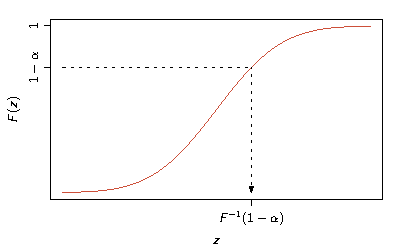
\includegraphics{Resources/Plots/unnamed-chunk-19-1} \end{center}
\normalsize
\end{frame}

\begin{frame}[fragile]{Quantile}
\phantomsection\label{quantile-1}
\begin{itemize}
\tightlist
\item
  Quantile der Normalverteilung etwa berechnet man in R bequem mit der
  Funktion \linebreak \texttt{qnorm(p,\ mean,\ sd)}.
\end{itemize}

\footnotesize

\begin{Shaded}
\begin{Highlighting}[]
\CommentTok{\# Quantile der Standardnormalverteilung}
\NormalTok{x }\OtherTok{\textless{}{-}} \FunctionTok{c}\NormalTok{(}\DecValTok{0}\NormalTok{, }\FloatTok{0.25}\NormalTok{, }\FloatTok{0.5}\NormalTok{, }\FloatTok{0.75}\NormalTok{, }\DecValTok{1}\NormalTok{)}
\FunctionTok{qnorm}\NormalTok{(}\AttributeTok{p =}\NormalTok{ x, }\AttributeTok{mean =} \DecValTok{0}\NormalTok{, }\AttributeTok{sd =} \DecValTok{1}\NormalTok{)}
\end{Highlighting}
\end{Shaded}

\begin{verbatim}
## [1]    -Inf -0.6745  0.0000  0.6745     Inf
\end{verbatim}

\normalsize

\vspace{0.5cm}
\QuizAcademy{Verteilungen 4}\endQuizAcademy
\end{frame}

\begin{frame}{\(\chi^2\)-Verteilung}
\phantomsection\label{chi2-verteilung}
\begin{itemize}
\tightlist
\item
  Ausgangspunkt sind \(n\) Zufallsvariablen \(Z_1,\ldots, Z_n\), die
  unabhängig und \(N(0,1)\)-verteilt sind. Die neue Zufallsvariable
  \[ X = Z_1^2 + Z_2^2 + \ldots + Z_n^2 \] folgt einer
  \hil{$\chi^2$-Verteilung}.
\item
  Die Anzahl der unabhängigen Zufallsvariablen \(n\) in dieser Summe
  wird als \hil{Freiheitsgrad} bezeichnet.
\item
  Erwartungswert und Varianz der \(\chi^2\)-Verteilung sind
  \begin{equation*}
  \mu=n \quad \text{und}\quad \sigma^2=2n.
  \end{equation*}
\item
  Die Freiheitsgrade \(n\) sind also Scharparameter der Verteilung.
  Daher schreibt man die \(\chi^2\)-Verteilung kompakt als
  \(\chi^2(n)\).
\item
  Weitere Details finden sich im Buch auf S.~135-138.
\end{itemize}
\end{frame}

\begin{frame}[fragile]{\(\chi^2\)-Verteilung}
\phantomsection\label{chi2-verteilung-1}
\framesubtitle{Erzeugen einer $\chi^2$-verteilten ZV in \R}

\footnotesize

\begin{Shaded}
\begin{Highlighting}[]
\NormalTok{Wiederholungen }\OtherTok{\textless{}{-}} \DecValTok{20000}
\NormalTok{FG }\OtherTok{\textless{}{-}} \DecValTok{7} \CommentTok{\# Freiheitsgrade der chi{-}Quadrat{-}Verteilung}
\NormalTok{Z  }\OtherTok{\textless{}{-}} \FunctionTok{replicate}\NormalTok{(Wiederholungen, }\FunctionTok{rnorm}\NormalTok{(FG)) }\CommentTok{\# 20000 Spalten à 7 N(0,1){-}ZVen}
\NormalTok{X  }\OtherTok{\textless{}{-}} \FunctionTok{colSums}\NormalTok{(Z}\SpecialCharTok{\^{}}\DecValTok{2}\NormalTok{) }\CommentTok{\# Spaltensummen der Quadrate}

\CommentTok{\# Histogramm der quadrierten Spaltensummen:}
\FunctionTok{hist}\NormalTok{(X, }\AttributeTok{freq =}\NormalTok{ F, }\AttributeTok{col=}\StringTok{"lightblue"}\NormalTok{, }\AttributeTok{breaks =} \DecValTok{40}\NormalTok{, }\AttributeTok{ylab=}\StringTok{"Dichte"}\NormalTok{, }\AttributeTok{main=}\StringTok{""}\NormalTok{)}
\NormalTok{grid }\OtherTok{\textless{}{-}} \FunctionTok{seq}\NormalTok{(}\DecValTok{0}\NormalTok{, }\DecValTok{60}\NormalTok{, }\FloatTok{0.03}\NormalTok{) }\CommentTok{\# x{-}Achse definieren}
\CommentTok{\# theoretische Dichte hinzufügen:}
\FunctionTok{lines}\NormalTok{(grid, }\FunctionTok{dchisq}\NormalTok{(}\AttributeTok{x =}\NormalTok{ grid, }\AttributeTok{df =}\NormalTok{ FG), }\AttributeTok{type =} \StringTok{\textquotesingle{}l\textquotesingle{}}\NormalTok{, }\AttributeTok{lwd =} \DecValTok{2}\NormalTok{, }\AttributeTok{col=}\StringTok{"tomato3"}\NormalTok{)}
\end{Highlighting}
\end{Shaded}

\normalsize
\vspace{-1.75em}

\footnotesize
\begin{center}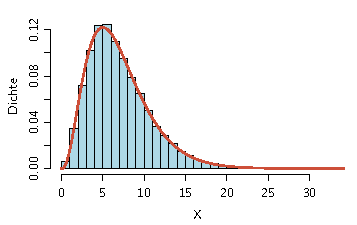
\includegraphics{Resources/Plots/unnamed-chunk-22-1} \end{center}
\normalsize
\end{frame}

\begin{frame}{\(t\)-Verteilung}
\phantomsection\label{t-verteilung}
\begin{itemize}
\tightlist
\item
  Bildet man aus unabhängigen Zufallsvariablen \(Z:\; N(0,1)\) und
  \(Y:\; \chi^2(n)\) den Quotienten
  \begin{equation} X=\frac{Z}{\sqrt{Y/n}}\label{tVtlg},
  \end{equation} dann ist \(X\) \hil{{\boldmath{$t$}}-verteilt} mit
  \(n\) Freiheitsgraden.
\item
  Die \(t\)-Verteilung hängt auch von den Freiheitsgraden \(n\) ab;
  kürze sie daher mit \(t(n)\) ab.
\item
  Der \hil{Erwartungswert} ist für \(n>1\) definiert und ist dann immer
  null. Die \hil{Varianz} ist \begin{equation*}
  \sigma^2=\frac{n}{n-2} \quad \text{für } n>2.
  \end{equation*}
\item
  Die \(t\)-Verteilung ist symmetrisch um \(\mu=0\), d.h.
  \(F(-x)= 1-F(x)\).
\end{itemize}
\end{frame}

\begin{frame}[fragile]{\(t\)-Verteilung}
\phantomsection\label{t-verteilung-1}
\footnotesize

\begin{Shaded}
\begin{Highlighting}[]
\NormalTok{grid }\OtherTok{\textless{}{-}} \FunctionTok{seq}\NormalTok{(}\SpecialCharTok{{-}}\DecValTok{3}\NormalTok{, }\DecValTok{3}\NormalTok{, .}\DecValTok{01}\NormalTok{)}
\FunctionTok{plot}\NormalTok{(}\AttributeTok{x =}\NormalTok{ grid, }\AttributeTok{y =} \FunctionTok{dnorm}\NormalTok{(grid), }\AttributeTok{type =} \StringTok{"l"}\NormalTok{, }
     \AttributeTok{col =} \StringTok{"tomato3"}\NormalTok{, }\AttributeTok{xlab =} \StringTok{""}\NormalTok{, }\AttributeTok{ylab =} \StringTok{""}\NormalTok{, }\AttributeTok{lwd =} \DecValTok{2}\NormalTok{)}
\FunctionTok{lines}\NormalTok{(}\AttributeTok{x =}\NormalTok{ grid, }\AttributeTok{y =} \FunctionTok{dt}\NormalTok{(grid, }\AttributeTok{df =} \DecValTok{4}\NormalTok{), }\AttributeTok{col =} \StringTok{"dodgerblue3"}\NormalTok{, }\AttributeTok{lwd =} \DecValTok{2}\NormalTok{)}
\FunctionTok{lines}\NormalTok{(}\AttributeTok{x =}\NormalTok{ grid, }\AttributeTok{y =} \FunctionTok{dt}\NormalTok{(grid, }\AttributeTok{df =} \DecValTok{2}\NormalTok{), }\AttributeTok{col =} \StringTok{"forestgreen"}\NormalTok{, }\AttributeTok{lwd =} \DecValTok{2}\NormalTok{)}
\end{Highlighting}
\end{Shaded}

\normalsize

\footnotesize
\begin{center}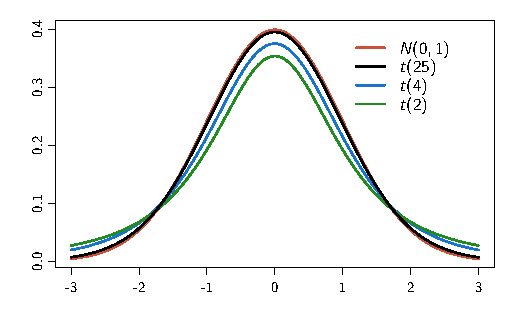
\includegraphics{Resources/Plots/tVtlg1x-1} \end{center}
\normalsize
\end{frame}

\begin{frame}[fragile]{\(t\)-Verteilung}
\phantomsection\label{t-verteilung-2}
\begin{itemize}
\tightlist
\item
  Die Abbildung zeigt \(f(x)\) der \(t\)-Verteilung für
  \(n=\{2, 4, 25\}\) und die Dichte der \(N(0,1)\)-Verteilung.
\item
  Für kleines \(n\) verläuft die \(t\)-Verteilung flacher als die
  \(N(0,1)\)-Verteilung.
\item
  Dieser Unterschied verringert sich aber mit wachsendem \(n\), so dass
  es ab \(n\geq 30\) zulässig ist, anstelle der \(t\)- die
  \(N(0,1)\)-Verteilung zu verwenden.
\end{itemize}

\footnotesize

\begin{Shaded}
\begin{Highlighting}[]
\NormalTok{x }\OtherTok{\textless{}{-}} \FunctionTok{seq}\NormalTok{(}\SpecialCharTok{{-}}\DecValTok{5}\NormalTok{,}\DecValTok{5}\NormalTok{)}
\FunctionTok{round}\NormalTok{(}\FunctionTok{dnorm}\NormalTok{(x) }\SpecialCharTok{{-}} \FunctionTok{dt}\NormalTok{(x, }\DecValTok{30}\NormalTok{), }\DecValTok{3}\NormalTok{)}
\end{Highlighting}
\end{Shaded}

\begin{verbatim}
##  [1]  0.000  0.000 -0.002 -0.003  0.004  0.003  0.004 -0.003 -0.002  0.000
## [11]  0.000
\end{verbatim}

\normalsize
\end{frame}

\begin{frame}{\(t\)-Verteilung}
\phantomsection\label{t-verteilung-3}
\exe

Finden Sie das folgende Quantil der \(t\)-Verteilung: \[t(0.95;30).\]
\endexe
\end{frame}

\begin{frame}{Anhang}
\phantomsection\label{anhang}
\framesubtitle{Geometrische Verteilung}

\begin{itemize}
\tightlist
\item
  Definitionsgemäß erhält man \(\mu\) der geometrischen Verteilung als
  \begin{equation*}
   \mu=\sum\limits^\infty_{x=0}x p q^x = p q
   \sum\limits^\infty_{x=1}x q^{x-1}.
  \end{equation*}
\item
  Um zu ermitteln, ob die Summe existiert und welchen Wert sie annimmt,
  wird der Ausdruck \(x q^{x-1}\) als Ableitung der Funktion \(q^x\)
  nach \(q\) geschrieben \[\dfrac{d}{dq}(q^x)=x q^{x-1}.\]
\item
  Bei endlichen Summen können die beiden Operationen \(\sum\) und
  \(\frac{d}{dp}\) vertauscht werden:
  \[ \sum\limits^\infty_{x=1}xq^{x-1}=\sum\limits^\infty_{x=1}\frac{d}{dq}(q^x) =\frac{d}{dq}\left(\sum\limits^\infty_{x=1}q^x\right). \]
\end{itemize}
\end{frame}

\begin{frame}{Anhang}
\phantomsection\label{anhang-1}
\framesubtitle{Geometrische Verteilung}

\begin{itemize}
\tightlist
\item
  Wegen \(|q|<1\) existiert \(\sum^\infty_{x=1}q^x\); aus der
  Summenformel für unendliche geometrische Reihen folgt
  \[\sum\limits^\infty_{x=1}q^x=\frac{q}{1-q}.\] Die Ableitung dieser
  Summe lautet
  \[\frac{d}{dq}\left(\frac{q}{1-q}\right)=\frac{1}{(1-q)^2}.\] Damit
  gilt \begin{equation*}
   \sum\limits^\infty_{x=1}x q^{x-1}=\frac{1}{(1-q)^2}\text{ für }
   |q|<1.
  \end{equation*}
\item
  Durch Einsetzen von
  \(\sum\limits^\infty_{x=1}x q^{x-1}=\frac{1}{(1-q)^2}\) in
  \(\mu=\sum\limits^\infty_{x=0}x p q^x = p q\sum\limits^\infty_{x=1}x q^{x-1}\)
  Daher folgt für den \hil{Erwartungswert} \vspace{-0.65em}
  \begin{equation*}
   \mu=\sum\limits^\infty_{x=0}x p q^x = p q\sum\limits^\infty_{x=1}x q^{x-1}=\frac{pq}{(1-q)^2}=\frac{q}{p}.
  \end{equation*}
\end{itemize}
\end{frame}

\begin{frame}{Anhang}
\phantomsection\label{anhang-2}
\framesubtitle{Geometrische Verteilung}

\begin{itemize}
\tightlist
\item
  Zur Berechnung der \hil{Varianz} folgt man dem Ansatz
  \[\sigma^2=\E(X^2)-\mu^2.\]
\item
  Da \(\mu\) bereits vorliegt, fehlt nur noch \(\E(X^2)\):
  \[ \E(X^2)=\sum\limits^\infty_{x=0}x^2 p q^x = p q \sum\limits^\infty_{x=1}x^2 q^{x-1}. \]
\item
  Die letzte Summe lässt sich wieder als Ableitung nach \(q\) darstellen
  \[ \sum\limits^\infty_{x=1}x^2 q^{x-1}=\frac{d}{dq} \left(\sum\limits^\infty_{x=1}x q^x\right)=\frac{d}{dq}\left( q\sum_{x=1}^\infty xq^{x-1}\right). \]
\end{itemize}
\end{frame}

\begin{frame}{Anhang}
\phantomsection\label{anhang-3}
\framesubtitle{Geometrische Verteilung}

\begin{itemize}
\tightlist
\item
  Ersetzt man jetzt die rechte Summe durch Gleichung
  \[\sum\limits^\infty_{x=1}x q^{x-1}=\frac{1}{(1-q)^2},\] folgt
  \begin{equation*}
   \sum_{x=1}^\infty x^2q^{x-1} =
   \frac{d}{dq}\left[\frac{q}{(1-q)^2}\right] = \frac{1+q}{(1-q)^3}
   \text{ für } |q|<1.
  \end{equation*}
\item
  Also ist \[ \E(X^2)=pq\frac{1+q}{(1-q)^3}=\frac{q(1+q)}{(1-q)^2}. \]
\item
  Die Varianz der geometrischen Verteilung folgt jetzt als
  \[\sigma^2 = \E(X^2) - \mu^2 = \frac{q(1+q)}{(1-q)^2} -  \frac{q^2}{p^2} = \frac{q}{(1-q)^2}= \frac{q}{p^2}.\]
\end{itemize}
\end{frame}

\begin{frame}{Anhang}
\phantomsection\label{anhang-4}
\framesubtitle{Hypergeometrische Verteilung}

\begin{itemize}
\tightlist
\item
  Für Erwartungswert und Varianz einer hypergeometrischen Verteilung ist
  folgende Umformung des Binomialkoeffizienten hilfreich. Es gilt
  \begin{equation*}
   \binom{M}{x}=\dfrac{M!}{x!(M-x)!}  =\dfrac{M(M-1)!}{x(x-1)!(M-x)!}=\dfrac{M}{x}\binom{M-1}{x-1}.
  \end{equation*}
\item
  Der Erwartungswert kann dann wie folgt aus seiner Definitionsgleichung
  ermittelt werden
  \[\mu = \sum_{x=0}^n x\frac{\binom{M}{x}\binom{N-M}{n-x}}{\binom{N}{n}} = \sum_{x=1}^n x
  \frac{\frac{M}{x}\binom{M-1}{x-1}\binom{N-M}{n-x}}{\frac{N}{n}\binom{N-1}{n-1}} = n\frac{M}{N}\sum_{x=1}^n
  \frac{\binom{M-1}{x-1}\binom{N-M}{n-x}}{\binom{N-1}{n-1}}.\]
\end{itemize}
\end{frame}

\begin{frame}{Anhang}
\phantomsection\label{anhang-5}
\framesubtitle{Hypergeometrische Verteilung}

\begin{itemize}
\tightlist
\item
  \(M/N\) stellt die Wahrscheinlichkeit dar, dass beim ersten Zug ein
  Element mit der Eigenschaft \(A\) eintritt.
\item
  Diese Wahrscheinlichkeit beträgt \(p\). Setzt man \(z=x-1\), kann die
  letzte Summe geschrieben werden
  \[ \sum_{x=1}^n \frac{\binom{M-1}{x-1}\binom{N-M}{n-x}}{\binom{N-1}{n-1}} = \sum_{z=0}^{n-1} \frac{\binom{M-1}{z}\binom{N-M}{n-1-z}}{\binom{N-1}{n-1}}. \]
\item
  Der letzte Bruch ist aber die Wahrscheinlichkeitsfunktion einer
  hypergeometrisch verteilten Zufallsvariablen \(Z\) mit den Parametern
  \(N-1,\) \(M-1\) und \(n-1: f(z|N-1, M-1, n-1)\).
\item
  Da ihre Summe über \(z=0,\ldots,n-1\) gleich eins ist, ist der
  Erwartungswert \(\mu\) einer hypergeometrisch verteilten
  Zufallsvariablen \begin{equation*}
   \mu=np.
  \end{equation*}
\end{itemize}
\end{frame}

\begin{frame}{Anhang}
\phantomsection\label{anhang-6}
\framesubtitle{Hypergeometrische Verteilung}

\begin{itemize}
\tightlist
\item
  Forme zur Ermittlung der \hil{Varianz} den Verschiebungssatz um:
  \[ \sigma^2=\E(X^2)-[\E(X)]^2=\E[X(X-1)]+\E(X)-[\E(X)]^2. \]
\item
  Beachtet man, dass außerdem gilt
  \[ \binom{M}{x}=\dfrac{M(M-1)}{x(x-1)}\binom{M-2}{x-2}\quad
  \text{und} \quad \binom{N}{n}=\dfrac{N(N-1)}{n(n-1)}\binom{N-2}{n-2}, \]
  ergibt sich
  \[ \E[X(X-1)]=\sum\limits^n_{x=0}x(x-1)\dfrac{\binom{M}{x}\binom{N-M}{n-x}}{\binom{N}{n}}= \dfrac{M(M-1)}{\frac{N(N-1)}{n(n-1)}}\sum\limits^n_{x=2}\dfrac{\binom{M-2}{x-2}\binom{N-M}{n-x} }{\binom{N-2}{n-2}}. \]
\item
  Setzt man jetzt \(z=x-2\) und stellt den Bruch vor dem letzten
  Summenzeichen um, erhält man
  \[ \E[X(X-1)]=\dfrac{p(M-1)n(n-1)}{(N-1)}\sum\limits^{n-2}_{z=0}\dfrac{\binom{M-2}{z} \binom{N-M}{n-2-z}}{\binom{N-2}{n-2}}, \text{ mit } p=\frac{M}{N}.
  \]
\end{itemize}
\end{frame}

\begin{frame}{Anhang}
\phantomsection\label{anhang-7}
\framesubtitle{Hypergeometrische Verteilung}

\begin{itemize}
\tightlist
\item
  Der letzte Bruch ist analog zu oben die Wahrscheinlichkeitsfunktion
  einer hypergeometrisch verteilten Zufallsvariablen mit \(N-2\),
  \(M-2\) und \(n-2\). Da auch ihre Summe eins ist, resultiert
  \[ \E[X(X-1)]=\dfrac{p(M-1)n(n-1)}{(N-1)}=\dfrac{n p(pN-1)(n-1)}{N-1}. \]
\item
  Es sind nun alle Terme bestimmt, so dass
  \[ \sigma^2=\dfrac{n p(p N-1)(n-1)}{N-1}+np-n^2p^2,\] oder nach
  einigen Umformungen \[  \sigma^2=np(1-p)\dfrac{N-n}{N-1}.\]
\end{itemize}
\end{frame}

\section{Grundzüge der
Stichprobentheorie}\label{grundzuxfcge-der-stichprobentheorie}

\begin{frame}{Stichproben und Stichprobenfunktion}
\phantomsection\label{stichproben-und-stichprobenfunktion}
\framesubtitle{Grundgesamtheit}

\begin{itemize}
\tightlist
\item
  Enthält eine Grundgesamtheit zu viele Elemente, sind \hil{Stichproben}
  notwendig.
\item
  Eine Grundgesamtheit kann endlich oder unendlich viele Elemente
  enthalten:

  \begin{itemize}
  \tightlist
  \item
    Theoretische Grundgesamtheiten sind oft (überabzählbar) unendlich,
    wie z.B. bei stetigen Zufallsvariablen.
  \item
    Reale Grundgesamtheiten sind meistens sehr groß, aber häufig endlich
    (z.B. deutsche Bevölkerung).
  \end{itemize}
\end{itemize}
\end{frame}

\begin{frame}{Stichproben und Stichprobenfunktion}
\phantomsection\label{stichproben-und-stichprobenfunktion-1}
\begin{itemize}
\tightlist
\item
  Bei unbekannter Verteilung in der Grundgesamtheit muss jede
  statistische Information hierüber durch Stichproben erhoben werden.
\item
  Das \hil{Ziehen einer Stichprobe} besteht darin, \(n\) Elemente aus
  der Grundgesamtheit auszuwählen.
\item
  So entsteht eine Stichprobe mit dem Umfang oder der Länge \(n\).
\item
  Um die Wahrscheinlichkeitstheorie für die Stichprobenanalyse nutzbar
  zu machen, muss das \hil{Auswahlverfahren} randomisiert sein.
\item
  Bei zufälliger Auswahl liegen \hil{Zufallsstichproben} vor.
\end{itemize}
\end{frame}

\begin{frame}{Stichproben und Stichprobenfunktion}
\phantomsection\label{stichproben-und-stichprobenfunktion-2}
\framesubtitle{QuizAcademy}
\QuizAcademy{Stichproben 1}\endQuizAcademy
\end{frame}

\begin{frame}{Stichproben und Stichprobenfunktion}
\phantomsection\label{stichproben-und-stichprobenfunktion-3}
\begin{itemize}
\tightlist
\item
  Jede zufällige Ziehung aus der Grundgesamtheit kann als eigenständige
  Zufallsvariable \(X_1,\ldots,X_n\) aufgefasst werden.
\item
  Ihre Verteilung hängt von der Verteilung von \(X\) in der
  Grundgesamtheit ab.
\item
  Die \(X_j\) bezeichnet man als \hil{Stichprobenvariablen}.
\item
  Wird das Element nach Ziehung wieder in die \glqq{}Urne\grqq{}
  zurückgelegt, spricht man von
  \hil{Zufallsstichproben mit Zurücklegen}.
\item
  Geschieht dies nicht, liegen \hil{Zufallsstichproben ohne Zurücklegen}
  vor (von denen wir im Folgenden abstrahieren wollen).
\item
  Je größer die Grundgesamtheit, desto bedeutungsloser die
  Unterscheidung ZmZ/ZoZ.
\end{itemize}
\end{frame}

\begin{frame}{Stichproben und Stichprobenfunktion}
\phantomsection\label{stichproben-und-stichprobenfunktion-4}
\begin{itemize}
\tightlist
\item
  Eine konkrete Zufallsstichprobe, auch als \hil{Stichprobenrealisation}
  bzw. \hil{Stichprobenergebnis} bezeichnet, sind also die Zahlen, die
  sich aus den Realisationen der \(X_j\) ergeben,
  \[ X_1=x_1, \quad X_2=x_2,\quad\ldots,X_n=x_n \] oder als \(n\)-Tupel
  geschrieben: \((x_1,\ldots,x_n).\)
\item
  Alle möglichen Stichproben stellen die Ausgänge und diese zusammen den
  \hil{Stichprobenraum} des Zufallsvorgangs \glqq{}Ziehen einer
  Stichprobe\grqq{} dar.
\end{itemize}
\end{frame}

\begin{frame}{Stichproben und Stichprobenfunktion}
\phantomsection\label{stichproben-und-stichprobenfunktion-5}
\rem[Uneingeschränkte Zufallsstichprobe]Jedes Element der
Grundgesamtheit besitzt dieselbe Wahrscheinlichkeit, in eine
Zufallsstichprobe mit dem Umfang \(n\) zu gelangen. \endrem

\begin{itemize}
\tightlist
\item
  ZmZ und ZoZ liefern immer \hil{uneingeschränkte Zufallsstichproben}
  und die \(X_j\) sind identisch verteilt wie \(X\).
\item
  Bei ZmZ sind die Stichprobenvariablen zusätzlich stochastisch
  unabhängig. Man erhält dann \hil{unabhängige Zufallsstichproben}.
\item
  Uneingeschränkte und unabhängige Zufallsstichproben heißen
  \hil{einfache Zufallsstichproben}.
\end{itemize}
\end{frame}

\begin{frame}{Stichproben und Stichprobenfunktion}
\phantomsection\label{stichproben-und-stichprobenfunktion-6}
\begin{itemize}
\tightlist
\item
  Eine Funktion \(T=T(X_1,\ldots,X_n),\) \(n\geq 1\), die nur von
  Stichprobenvariablen, nicht aber von unbekannten Parametern abhängt,
  heißt \hil{Stichprobenfunktion} bzw. \hil{Statistik}.
\item
  Stichprobenfunktionen sollen Stichprobenergebnisse in aussagekräftige,
  einfache statistische Größen überführen.
\item
  So stellen
  \[ T=\frac{1}{n}\sum\limits^n_{j=1} X_j \ \ \text{oder} \ \ T=X_1-5 \]
  Stichprobenfunktionen bzw. Statistiken dar, nicht aber
  \[Z=\frac{X-\mu}{\sigma},\] wenn \(\mu\) und \(\sigma\) unbekannt
  sind.
\end{itemize}
\end{frame}

\begin{frame}{Stichproben und Stichprobenfunktion}
\phantomsection\label{stichproben-und-stichprobenfunktion-7}
\begin{itemize}
\tightlist
\item
  Da die Argumente von \(T\) Zufallsvariablen sind, ist \(T\) selbst
  eine Zufallsvariable, deren Verteilung \hil{Stichprobenverteilung}
  heißt.
\item
  Die Varianz der Stichprobenverteilung nennt man \hil{Fehlervarianz},
  die positive Wurzel hieraus \hil{Standardfehler}.
\item
  Eine Realisation von \(T\) aufgrund einer konkreten Stichprobe wird
  mit \[t=T(x_1,\ldots,x_n)\] bezeichnet.
\item
  Im Folgenden betrachten wir einige spezielle Stichprobenverteilungen.
\end{itemize}
\end{frame}

\begin{frame}{Stichprobenverteilung des arithmetischen Mittels}
\phantomsection\label{stichprobenverteilung-des-arithmetischen-mittels}
\begin{itemize}
\tightlist
\item
  Ziehen aller möglicher Stichproben aus einer Grundgesamtheit und
  jeweiliges Berechnen der Stichprobenfunktion arithmetisches Mittel,
  \(\bar{X}=\frac{1}{n}\sum^n_{j=1} X_j\), liefert dessen
  \hil{Stichprobenverteilung}.
\item
  Wir betrachten zunächst Erwartungswert und Varianz der Verteilung.
\item
  Der Erwartungswert von \(\bar{X}\) ist
  \begin{equation} \E(\bar{X})=\E\left(\frac{1}{n}\sum_{j=1}^n X_j\right) = \frac{1}{n}\sum_{j=1}^n \E(X_j)= \frac{n}{n}\mu=\mu,
  \label{EWMWsrs}
  \end{equation} eine Vereinfachung von \eqref{EW}, da nun wegen der
  identischen Verteilung alle Erwartungswerte gleich sind.
\end{itemize}
\end{frame}

\begin{frame}{Stichprobenverteilung des arithmetischen Mittels}
\phantomsection\label{stichprobenverteilung-des-arithmetischen-mittels-1}
\begin{itemize}
\item
  Bei einfachen Stichproben erhält man die Fehlervarianz als
  \begin{align}
  \var(\bar{X}) =\sigma^2_{\bar{X}}&=\var\left(\frac{1}{n}\sum_{j=1}^n X_j\right)
  \stackrel{\eqref{varlinTrafo}}{=} \frac{1}{n^2}\sum_{j=1}^n\var(X_j) \notag\\
  & =\frac{1}{n^2}\sum_{j=1}^n
  \sigma^2 =\frac{1}{n}\sigma^2.\label{varMWsrs}
  \end{align}
\item
  Um die Verteilung von \(\bar{X}\) zu bestimmen, muss unterschieden
  werden, ob die Verteilung für \(X\) in der Grundgesamtheit bekannt ist
  oder nicht.
\item
  Ist \(X\) \hil{normalverteilt} mit \(\mu\) und \(\sigma^2\), dann ist
  aufgrund der Reproduktivitätseigenschaft der Normalverteilung auch
  \(\bar{X}\) normalverteilt mit (bei Unabhängigkeit) den oben
  abgeleiteten Parametern
  \[ \mu_{\bar{X}}=\mu \quad \text{und} \quad \sigma^2_{\bar{X}}=\frac{\sigma^2}{n}. \]
\end{itemize}
\end{frame}

\begin{frame}[fragile]{Stichprobenverteilung des arithmetischen Mittels}
\phantomsection\label{stichprobenverteilung-des-arithmetischen-mittels-2}
\framesubtitle{Beispiele}

\xmpl[Körpergröße deutscher Männer]Die Körpergröße deutscher Männer sei
in der Grundgesamtheit normalverteilt mit \(\mu=178\) cm und
\(\sigma^2=64\text{ cm}^2\). Das Stichprobenmittel \(\bar{X}\) ist dann
normalverteilt mit \(\mu_{\bar{X}}=178\) und
\(\sigma^2_{\bar{X}}=64/n\). Wird eine Stichprobe mit dem Umfang
\(n=100\) gezogen, ist \(\sigma^2_{\bar{X}}=64/100=0.64\).\mps Die
Wahrscheinlichkeit, dass eine Stichprobe einen Mittelwert von
\(\bar{x}=180\) oder größer liefert, ist mit
\texttt{1-pnorm(180,\ 178,\ sqrt(0.64))} \(=0.0062\) \begin{align*}
  P(\bar{X}\geq 180) & =
  %P\left(Z\geq\frac{180-\mu}{\sigma/\sqrt{n}}\right)=P\left(Z\geq \frac{180-178}{0.8}\right)\\
  %& =P(Z\geq2.5) = 1-P(Z<2.5)=1-0.9938=
  0.0062.
 \end{align*} \endxmpl
\end{frame}

\begin{frame}[fragile]{Stichprobenverteilung des arithmetischen Mittels}
\phantomsection\label{stichprobenverteilung-des-arithmetischen-mittels-3}
\xmpl[*]

\footnotesize

\begin{Shaded}
\begin{Highlighting}[]
\NormalTok{mu   }\OtherTok{\textless{}{-}} \DecValTok{178}\NormalTok{; sigma }\OtherTok{\textless{}{-}} \DecValTok{8}\NormalTok{; N }\OtherTok{\textless{}{-}} \DecValTok{100} \CommentTok{\# EW, Standardabw., Stichprobengröße}
\NormalTok{grid }\OtherTok{\textless{}{-}} \FunctionTok{seq}\NormalTok{(mu }\SpecialCharTok{{-}} \DecValTok{3}\NormalTok{, mu }\SpecialCharTok{+} \DecValTok{3}\NormalTok{, .}\DecValTok{01}\NormalTok{)}
\CommentTok{\# ziehe 5000 Stichproben der Größe 100 und berechne deren Stichprobenmittel:}
\NormalTok{est  }\OtherTok{\textless{}{-}} \FunctionTok{colMeans}\NormalTok{(}\FunctionTok{replicate}\NormalTok{(}\DecValTok{5000}\NormalTok{, }\FunctionTok{rnorm}\NormalTok{(N, mu, sigma)))}
\FunctionTok{hist}\NormalTok{(est, }\AttributeTok{freq =}\NormalTok{ F, }\AttributeTok{col =} \StringTok{"lightblue"}\NormalTok{, }\AttributeTok{breaks =} \DecValTok{40}\NormalTok{, }\AttributeTok{ylab =} \StringTok{"Dichte"}\NormalTok{, }\AttributeTok{main =} \StringTok{""}\NormalTok{)}
\FunctionTok{lines}\NormalTok{(}\AttributeTok{x =}\NormalTok{ grid, }\AttributeTok{y =} \FunctionTok{dnorm}\NormalTok{(grid, mu, sigma}\SpecialCharTok{/}\FunctionTok{sqrt}\NormalTok{(N)), }\AttributeTok{col =} \StringTok{"tomato3"}\NormalTok{, }\AttributeTok{lwd =} \DecValTok{2}\NormalTok{)}
\end{Highlighting}
\end{Shaded}

\begin{center}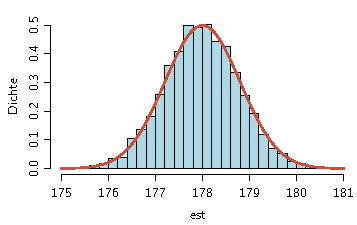
\includegraphics{Resources/Plots/unnamed-chunk-23-1} \end{center}
\normalsize
\endxmpl
\end{frame}

\begin{frame}{Stichprobenverteilung des arithmetischen Mittels}
\phantomsection\label{stichprobenverteilung-des-arithmetischen-mittels-4}
\framesubtitle{Aufgaben}
\exe

Die vom Unternehmen A hergestellten Glühlampen besitzen eine
normalverteilte Lebensdauer mit einem Erwartungswert von 800 Stunden und
einer Standardabweichung von 40 Stunden.\mps Eine Geschäftsfiliale
bekommt eine Lieferung von 100 Glühlampen. Wie groß ist die
Wahrscheinlichkeit, dass die durchschnittliche Lebensdauer weniger als
790 Stunden beträgt? \endexe
\end{frame}

\begin{frame}{Das Gesetz der großen Zahlen}
\phantomsection\label{das-gesetz-der-grouxdfen-zahlen}
Was passiert mit dieser Verteilung, wenn \(n\) sehr groß wird? Betrachte
hierzu \(\bar{X}\) als Folge von Zufallsvariablen und schreibe deswegen
\(\bar{X}(n)\). \defn[Schwaches Gesetz der großen Zahlen]\label{GdgZ}
Das \hil{schwache Gesetz der großen Zahlen} lautet
\[ \lim\limits_{n\rightarrow\infty} P[|\bar{X}(n)-\mu|>\varepsilon] =0 \quad \text{bzw.} \quad \lim\limits_{n\rightarrow\infty} P[|\bar{X}(n)-\mu|<\varepsilon] =1. \]
\enddefn \vspace{0.5cm} Mehr hierzu im Buch auf S.~171-176.
\end{frame}

\begin{frame}{Zentraler Grenzwertsatz von Lindeberg-Levy}
\phantomsection\label{zentraler-grenzwertsatz-von-lindeberg-levy}
Der \hil{zentrale Grenzwertsatz von Lindeberg-Levy} liefert bei
\hil{unbekannter Verteilung} von \(X\) eine Approximation der Verteilung
von \(\bar{X}\). \defn[Zentraler Grenzwertsatz von Lindeberg-Levy]Die
Verteilung der standardisierten Summe und des standardisierten
Durchschnitts, also \begin{equation}\label{ZGWS}
\frac{\tilde{S}(n)-n\mu}{\sqrt{n}\sigma} \quad \text{bzw.}\quad \frac{\bar{X}(n)-\mu}{\sigma/\sqrt{n}} \to_DN(0,1),
\end{equation} d.h., konvergiert für \(n\rightarrow\infty\) gegen die
\hil{Standardnormalverteilung} \(N(0,1)\). \enddefn \vspace{0.5cm}
Dieser basiert auf der Annahme, dass \(X_1,\ldots,X_n\) unabhängig
identisch verteilt sind mit \(\E(X_j)=\mu\) und \(\var(X_j)=\sigma^2>0\)
für alle \(j\). Mehr nicht!
\end{frame}

\begin{frame}{Zentraler Grenzwertsatz von Lindeberg-Levy}
\phantomsection\label{zentraler-grenzwertsatz-von-lindeberg-levy-1}
Aus dem zentralen Grenzwertsatz von \hil{Lindeberg-Levy} folgt daher für
ein großes \(n\), dass

\begin{enumerate}
[(a)]
\tightlist
\item
  die Summe \(\tilde{S}(n)\) asymptotisch normalverteilt
  \(N(n \mu, n \sigma^2)\) und
\item
  der Durchschnitt \(\bar{X}(n)\) asymptotisch normalverteilt
  \(N\left(\mu, \sigma^2/n\right)\)
\end{enumerate}

ist. Siehe \texttt{clt.R}.
\end{frame}

\begin{frame}{Zentraler Grenzwertsatz von Lindeberg-Levy}
\phantomsection\label{zentraler-grenzwertsatz-von-lindeberg-levy-2}
\framesubtitle{Aufgaben}
\exe

Die maximale Traglast eines der beiden Besucheraufzüge im
Reichstagsgebäude in Berlin beträgt 4000 kg. Nach Herstellerangaben
entspricht dies einer Kapazität von 45 Personen. Das Gewicht der
Personen, die den Aufzug benutzen, beträgt im Durchschnitt 88 kg bei
einer Varianz von 16 kg\(^2\).\mps Wie groß ist die Wahrscheinlichkeit,
dass bei 45 Personen die maximale Traglast überschritten wird? \endexe
\end{frame}

\begin{frame}{Zentraler Grenzwertsatz von Lindeberg-Levy}
\phantomsection\label{zentraler-grenzwertsatz-von-lindeberg-levy-3}
\framesubtitle{Aufgaben}

\exe
2500 Unternehmensberater wurden bzgl. ihres Jahreseinkommens befragt. Es
ergab sich ein Durchschnittseinkommen von 51.800 Euro mit einer
Standardabweichung von 4000 Euro.\mps Wie groß ist die
Wahrscheinlichkeit, dass bei einer Stichprobe im Umfang von \(n=30\) der
Mittelwert um höchstens 500 Euro vom Erwartungswert abweicht? \endexe
\end{frame}

\begin{frame}{Stichprobenverteilung des Anteilswertes}
\phantomsection\label{stichprobenverteilung-des-anteilswertes}
Siehe Buch ab S.~192.
\end{frame}

\begin{frame}{\large Verteilung von Quotienten aus
Stichprobenfunktionen}
\phantomsection\label{verteilung-von-quotienten-aus-stichprobenfunktionen}
\begin{itemize}
\tightlist
\item
  Aus \eqref{stdNormalTrafo} folgt, dass der standardisierte Mittelwert
  \begin{equation}\label{ZN01}
  Z=\frac{\bar{X}-\mu}{\sigma/\sqrt{n}}\sim N(0,1),
  \end{equation} also \(N(0,1)\)-verteilt ist, wenn \(X\) normalverteilt
  ist.
\item
  Dieses Ergebnis setzt aber die Kenntnis der Varianz \(\sigma^2\) von
  \(X\) in der Grundgesamtheit voraus. Ist \(\sigma^2\) \hil{unbekannt},
  ist \(Z\) keine Stichprobenfunktion mehr.
\item
  Ersetzt man \(\sigma^2\) durch die \hil{Stichprobenvarianz}
  \[S^2=\frac{1}{n-1}\sum_{i=1}^n(X_i-\bar{X})^2,\] geht \(Z\) über in
  \[ Z(t)=\frac{\bar{X}-\mu}{S/\sqrt{n}}. \]
\end{itemize}
\end{frame}

\begin{frame}{\large Verteilung von Quotienten aus
Stichprobenfunktionen}
\phantomsection\label{verteilung-von-quotienten-aus-stichprobenfunktionen-1}
\begin{itemize}
\tightlist
\item
  \(Z(t)\) ist jetzt aber nicht mehr standardnormalverteilt.
\item
  \(Z(t)\) ist bei bekanntem \(\mu\) eine Stichprobenfunktion.
\item
  Um das Verteilungsgesetz von \(Z(t)\) zu entwickeln, erweitere
  \[Z(t)=\frac{\bar{X}-\mu}{S/\sqrt{n}}=\frac{\overset{N(0,1),\; s.~\eqref{ZN01}}{\overbrace{\sqrt{n}\frac{\bar{X}-\mu}{\sigma}}}}{
  \sqrt{\underset{\chi^2}{\underbrace{{\frac{(n-1)S^2}{\sigma^2}}}}\Bigl/n-1}}.
   \label{tVert}\]
\item
  Der Zähler \(Z\) in \(Z(t)\) ist standardnormalverteilt.
\item
  \((n-1)S^2/\sigma^2\) ist bei normalverteiltem \(X\)
  \(\chi^2\)-verteilt mit \(n-1\) Freiheitsgraden.
\end{itemize}
\end{frame}

\begin{frame}{\large Verteilung von Quotienten aus
Stichprobenfunktionen}
\phantomsection\label{verteilung-von-quotienten-aus-stichprobenfunktionen-2}
\begin{itemize}
\tightlist
\item
  Wir erinnern uns (vgl.~\eqref{tVtlg}), dass der Quotient aus einer
  \(N(0,1)\)- und der Wurzel einer \(\chi^2\)-verteilten
  Zufallsvariablen geteilt durch ihre Freiheitsgerade \hil{$t$-verteilt}
  ist, sofern die ZVen \hil{unabhängig} sind.
\item
  Da \(\bar{X}\) und \(S^2\) auf derselben Stichprobe beruhen, hängt
  \(S^2\) von \(\bar{X}^2\) ab. Die beiden Zufallsvariablen \(\bar{X}\)
  und \(S^2\) sind daher i.A.~stochastisch abhängig.
\item
  Eine Ausnahme liegt vor, wenn \(X\) in der Grundgesamtheit
  \hil{normalverteilt} ist: Dann sind \(\bar{X}\) und \(S^2\)
  unabhängig.
\item
  Ist also \(X\) in der Grundgesamtheit normalverteilt, dann folgt
  \(Z(t)\) einer \(t\)-Verteilung mit \(n-1\) Freiheitsgraden.
\end{itemize}
\end{frame}

\begin{frame}{\large Verteilung von Quotienten aus
Stichprobenfunktionen}
\phantomsection\label{verteilung-von-quotienten-aus-stichprobenfunktionen-3}
\framesubtitle{Beispiel}
\xmpl

Aus einer normalverteilten Grundgesamtheit mit \(\mu=10\) und
unbekannter Varianz wird eine Stichprobe mit \(n=9\) gezogen.\mps Die
Stichprobenvarianz sei \(s^2=9\). Die Variable
\[ Z(t)=\frac{\bar{X}-10}{3/\sqrt{9}}=\bar{X}-10 \] ist \(t\)-verteilt
mit \(n-1=8\) Freiheitsgraden. \endxmpl
\end{frame}

\begin{frame}{\large Verteilung von Quotienten aus
Stichprobenfunktionen}
\phantomsection\label{verteilung-von-quotienten-aus-stichprobenfunktionen-4}
\framesubtitle{QuizAcademy}
\QuizAcademy{Stichproben 2}\endQuizAcademy
\end{frame}

\begin{frame}{\large Verteilung von Quotienten aus
Stichprobenfunktionen}
\phantomsection\label{verteilung-von-quotienten-aus-stichprobenfunktionen-5}
\xmpl

Das Stichprobenmittel für \(n=9\) betrage \(\bar{x}=12\), so dass
\(Z(t)=2\). Die Wahrscheinlichkeit dafür, dass \(\bar{X}\) kleiner
gleich 12 ist, beträgt \[ P(\bar{X}\leq 12)=P[Z(t)\leq 2]. \]
\(P[Z(t)\leq 2]\) ermitteln wir in \R durch \texttt{pt(2, 8)} = 0.9597.
\endxmpl
\end{frame}

\begin{frame}{\large Verteilung von Quotienten aus
Stichprobenfunktionen}
\phantomsection\label{verteilung-von-quotienten-aus-stichprobenfunktionen-6}
\begin{itemize}
\tightlist
\item
  Für ein großes \(n\) ist die zuvor vorgestellte Vorgehensweise auch
  bei \hil{unbekannter Verteilung} von \(X\) und unbekannter Varianz
  gültig.
\item
  Aufgrund des Gesetzes der großen Zahlen lässt sich die Varianz für
  großes \(n\) gut über die Stichprobenvarianz approximieren, also
  \(S^2\approx\sigma^2\).
\item
  Also gilt
  \[ Z(t)=\frac{\bar{X}-\mu}{S/\sqrt{n}}\approx\frac{\bar{X}-\mu}{\sigma/\sqrt{n}}\sim N(0,1), \]
  d.h.~wir verwenden den Zentralen Grenzwertsatz.
\end{itemize}
\end{frame}

\section{Statistische
Schätzverfahren}\label{statistische-schuxe4tzverfahren}

\begin{frame}{Statistische Schätzverfahren}
\phantomsection\label{statistische-schuxe4tzverfahren-1}
\begin{itemize}
\tightlist
\item
  Bei vielen empirischen Untersuchungen sind die Parameter in der
  Grundgesamtheit unbekannt.
\item
  Die \hil{statistische Schätztheorie} befasst sich mit Möglichkeiten,
  diese Parameter aus Stichproben zu schätzen.
\item
  Die Quantifizierung der Sicherheit solcher Schätzungen nutzt die
  Ergebnisse der Stichprobentheorie.
\item
  Die Schätzung eines unbekannten Parameters \(\theta\) einer
  Grundgesamtheit wird mit einer Stichprobenfunktion durchgeführt, die
  jetzt \hil{Schätzfunktion} oder \hil{Schätzer} heißt.
\item
  Schätzer haben also auch eine Verteilung.
\end{itemize}
\end{frame}

\begin{frame}{Statistische Schätzverfahren}
\phantomsection\label{statistische-schuxe4tzverfahren-2}
\framesubtitle{Eigenschaften von Schätzern}

\begin{itemize}
\tightlist
\item
  Die Schätzfunktion lautet
  \[ \hat{\theta}=T_{\theta} (X_1,\ldots,X_n).\] \(\hat{\theta}\) ist
  dann eine Zufallsvariable mit Schätzwerten, die unterschiedlich stark
  von \(\theta\) abweichen.
\item
  Einsetzen von Stichprobenrealisationen in den Schätzer liefert einen
  konkreten Schätzwert. Dieser Schätzwert heißt \hil{Punktschätzung}.
\item
  Eine \hil{Intervallschätzung} liefert eine Intervallvorschrift, die
  mit vorgegebener Wahrscheinlichkeit den unbekannten Parameter
  \(\theta\) enthält.
\end{itemize}
\end{frame}

\begin{frame}{Statistische Schätzverfahren}
\phantomsection\label{statistische-schuxe4tzverfahren-3}
\framesubtitle{Eigenschaften von Schätzern}

\begin{itemize}
\tightlist
\item
  Wir suchen Schätzer, die bestimmte Qualitätskriterien erfüllen.
\item
  Die Abweichung \(\hat{\theta}-\theta\) heißt \hil{Schätzfehler}.
\item
  Eine wünschenswerte Eigenschaft ist, dass der Erwartungswert des
  Schätzfehlers für jeden Stichprobenumfang \(n\) null ist.
\item
  Formal:
  \[ \E(\hat{\theta}_n-\theta)=0 \quad \text{oder}\quad \E(\hat{\theta}_n)=\theta \quad  \text{für alle } n. \]
\item
  Ein Schätzer \(\hat{\theta}_n\), die dieses Kriterium erfüllt, heißt
  \hil{erwartungstreu}, \hil{unverzerrt} oder \hil{unbiased}.
\item
  Andernfalls \hil{nicht erwartungstreu} bzw. \hil{verzerrt}.
\item
  Es gibt oft mehrere erwartungstreue Schätzer.
\item
  Aus der Klasse erwartungstreuer Schätzer liegt es nahe, den mit der
  \hil{kleinsten Varianz} zu bestimmen.
\end{itemize}
\end{frame}

\begin{frame}{Statistische Schätzverfahren}
\phantomsection\label{statistische-schuxe4tzverfahren-4}
\framesubtitle{Eigenschaften von Schätzern - QuizAcademy}
\QuizAcademy{Schätzfrage}\endQuizAcademy
\end{frame}

\begin{frame}{Statistische Schätzverfahren}
\phantomsection\label{statistische-schuxe4tzverfahren-5}
\framesubtitle{Eigenschaften von Schätzern}

\begin{itemize}
\tightlist
\item
  Hier sind die Stichprobenverteilungen für zwei erwartungstreue
  Schätzer \(\hat{\theta}_{1,n}\) und \(\hat{\theta}_{2,n}\)
  dargestellt. \(\hat{\theta}_{1,n}\) ist effizienter als
  \(\hat{\theta}_{2,n}\), da
  \(\var(\hat{\theta}_{2,n})>\var(\hat{\theta}_{1,n})\).
\end{itemize}

\footnotesize
\begin{center}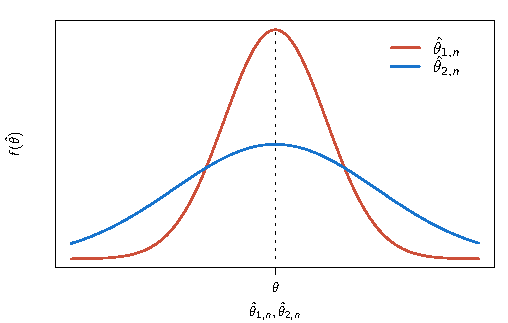
\includegraphics{Resources/Plots/unnamed-chunk-24-1} \end{center}
\normalsize
\end{frame}

\begin{frame}{Statistische Schätzverfahren}
\phantomsection\label{statistische-schuxe4tzverfahren-6}
\framesubtitle{Eigenschaften von Schätzern}

\begin{itemize}
\tightlist
\item
  Den Vorteil einer erwartungstreuen und effizienten Schätzung kann man
  analytisch zeigen. Die Tschebyscheff-Ungleichung
  \eqref{Tschebyscheff1} liefert
  \[ P(|X-\mu|\geq \varepsilon)\leq \frac{\sigma^2}{\varepsilon^2}. \]
\item
  Setzt man \(X=\hat{\theta}\), \(\mu=\E(\hat{\theta})=\theta\) und
  \(\sigma^2=\var(\hat{\theta})\) folgt
  \[ P(|\hat{\theta}-\theta|\geq\varepsilon)\leq \dfrac{\var(\hat{\theta})}{\varepsilon^2}. \]
\item
  Je kleiner \(\var(\hat{\theta})\), desto geringer wird die
  Wahrscheinlichkeit, dass der absolute Schätzfehler
  \(|\hat{\theta}-\theta|\) größer als \(\varepsilon\) ist.
\item
  Daher ist \(\hat{\theta}_{1,n}\) dem Schätzer \(\hat{\theta}_{2,n}\)
  vorzuziehen.
\end{itemize}
\end{frame}

\begin{frame}{Statistische Schätzverfahren}
\phantomsection\label{statistische-schuxe4tzverfahren-7}
\framesubtitle{Eigenschaften von Schätzern}

\begin{itemize}
\tightlist
\item
  Eine weitere wünschenswerte Eigenschaft von erwartungstreuen Schätzern
  ist die Konvergenz der Varianz mit zunehmendem \(n\) gegen null.
\item
  Für \(n\rightarrow\infty\) folgt
  \[ \lim\limits_{n\rightarrow\infty} P(|\hat{\theta}_n-\theta|\geq\varepsilon)=0 \quad \text{für } \lim\limits_{n\rightarrow\infty}\var(\hat{\theta}_n)=0. \]
\item
  Schätzfunktionen mit der Eigenschaft
  \[\lim\limits_{n\rightarrow\infty} P(|\hat{\theta}_n-\theta|<\varepsilon)=1 \]
  heißen (schwach) \hil{konsistent}.
\item
  Diese Eigenschaft entspricht formal dem Gesetz der großen Zahlen
  (siehe~\ref{GdgZ}).
\end{itemize}
\end{frame}

\begin{frame}{Statistische Schätzverfahren}
\phantomsection\label{statistische-schuxe4tzverfahren-8}
\framesubtitle{Eigenschaften von Schätzern}

\begin{itemize}
\tightlist
\item
  Bei verzerrten Schätzern ist der Erwartungswert des Schätzfehlers
  nicht null: \[\E(\hat{\theta}_n) \neq\theta.\]
\item
  Die Differenz \(\E(\hat{\theta}_n)-\theta\) misst die
  \hil{Verzerrung}.
\item
  Bei einigen verzerrten Schätzern stellt sich für
  \(n\rightarrow\infty\) Erwartungstreue ein:
  \[ \lim\limits_{n\rightarrow\infty}\E(\hat{\theta}_n - \theta)=0 \quad \text{bzw.}\quad \lim\limits_{n\rightarrow\infty} \E(\hat{\theta}_n) =\theta. \]
\item
  Diesen Fall nennt man \hil{asymptotische Erwartungstreue}.
\item
  Auch asymptotisch erwartungstreue Schätzer können konsistent sein.
\item
  Betrachte hierzu den \hil{mittleren quadratischen Fehler} (MSE)
  \[ \text{MSE}(\hat{\theta}_n)=\E[(\hat{\theta}_n-\theta)^2]. \]
\end{itemize}
\end{frame}

\begin{frame}{Statistische Schätzverfahren}
\phantomsection\label{statistische-schuxe4tzverfahren-9}
\framesubtitle{Mean Squared Error}

\begin{itemize}
\tightlist
\item
  Das Buch auf S.~214 zeigt, dass der mittlere quadratische Fehler die
  Summe von Varianz \(\var(\hat{\theta}_n)\) und quadrierter Verzerrung
  \([\E(\hat{\theta}_n)-\theta]^2\) ist:
  \[ \text{MSE}(\hat{\theta}_n)=\var(\hat{\theta}_n)+[\E(\hat{\theta}_n)-\theta]^2. \]
\item
  Der verzerrte Schätzer ist konsistent, wenn gilt
  \[ \lim\limits_{n\rightarrow\infty}\text{MSE}(\hat{\theta}_n)= \lim\limits_{n\rightarrow\infty} \var(\hat{\theta}_n)+ \lim\limits_{n\rightarrow\infty}[\E(\hat{\theta}_n)-\theta]^2 =0. \]
\item
  Da weder die Varianz noch die quadrierte Verzerrung negativ werden
  können, müssen beide Grenzwerte null sein.
\item
  Damit ist eine hinreichende Bedingung für \hil{Konsistenz} gefunden.
  \[ \text{\blue{(a)}} \;\lim\limits_{n\rightarrow\infty}[\E(\hat{\theta}_n)-\theta]^2=0 \quad \text{und}\quad \text{\blue{(b)}} \; \lim\limits_{n\rightarrow\infty} \var(\hat{\theta}_n)=0 \]
\end{itemize}
\end{frame}

\begin{frame}{Intervallschätzung}
\phantomsection\label{intervallschuxe4tzung}
\framesubtitle{Mean Squared Error}

\xmpl[$\bar{X}$ als Schätzer für $\mu$]\(\bar{X}\) ist ein
erwartungstreuer Schätzer für \(\mu\). Der \(\text{MSE}(\bar{X})\) ist
daher gleich der Varianz, \begin{align*}
\text{MSE}(\bar{X})&= \var(\bar{X})\\&\stackrel{\eqref{varMWsrs}}{=}\frac{\sigma^2}{n}.
\end{align*}

\endxmpl
\end{frame}

\begin{frame}[fragile]{Statistische Schätzverfahren}
\phantomsection\label{statistische-schuxe4tzverfahren-10}
\framesubtitle{Konsistenz}

\xmpl[Werfen eines Würfel]Die ZV \(X\) sei die realisierte Augenzahl
beim Werfen eines Würfels. Es gilt \begin{align*}
\E(\bar{X}) = \frac{1}{n}\sum_{j=1}^n \E(X_j) = \E(X_j) = \mu \stackrel{\eqref{EWWuerfel}}{=} 3.5
\end{align*} sowie \begin{align*}
\MSE(\bar{X}) = \var(\bar{X}) = \frac{\sigma^2}{n} \stackrel{\eqref{VarWuerfel}}{\approx} \frac{2.9167}{n}
\end{align*}

\footnotesize

\begin{Shaded}
\begin{Highlighting}[]
\NormalTok{n    }\OtherTok{\textless{}{-}} \DecValTok{300} \CommentTok{\# 300 Würfe}
\NormalTok{Xbar }\OtherTok{\textless{}{-}} \FunctionTok{cumsum}\NormalTok{(}\FunctionTok{sample}\NormalTok{(}\DecValTok{1}\SpecialCharTok{:}\DecValTok{6}\NormalTok{, }\AttributeTok{size =}\NormalTok{ n, }\AttributeTok{replace =}\NormalTok{ T)) }\SpecialCharTok{/} \DecValTok{1}\SpecialCharTok{:}\NormalTok{n }\CommentTok{\# Kumulierte Mittel}
\FunctionTok{head}\NormalTok{(Xbar) }
\end{Highlighting}
\end{Shaded}

\begin{verbatim}
## [1] 1.000 1.500 2.667 2.750 3.400 3.833
\end{verbatim}

\normalsize
\endxmpl
\end{frame}

\begin{frame}{Statistische Schätzverfahren}
\phantomsection\label{statistische-schuxe4tzverfahren-11}
\framesubtitle{Konsistenz}

\xmpl[*]

\footnotesize
\begin{center}\includegraphics{Resources/Plots/unnamed-chunk-26-1} \includegraphics{Resources/Plots/unnamed-chunk-26-2} \end{center}
\normalsize
\endxmpl
\end{frame}

\begin{frame}{Statistische Schätzverfahren}
\phantomsection\label{statistische-schuxe4tzverfahren-12}
\framesubtitle{Konsistenz}

\begin{itemize}
\tightlist
\item
  Man spricht dann von \hil{Konvergenz im quadratischen Mittel}.
\item
  Im quadratischen Mittel konvergente Schätzer sind immer auch
  mindestens asymptotisch erwartungstreu.
\item
  Konsistenz ist eine Mindestanforderung für einen guten Schätzer.
\end{itemize}

\xmpl[Verzerrter, aber konsistenter Schätzer]Das Mittel
\(\widetilde{X} = \frac{1}{n+3}\sum_{i=1}^n X_i\) ist ein verzerrter,
jedoch konsistenter Schätzer für den Erwartungswert. \begin{align*}
  \E(\widetilde{X}) = \frac{n}{n+3}\mu \neq \mu
\end{align*} \endxmpl
\end{frame}

\begin{frame}{Statistische Schätzverfahren}
\phantomsection\label{statistische-schuxe4tzverfahren-13}
\framesubtitle{Konsistenz}

\xmpl[*]Überprüfung der Bedingung \blue{(a)}: \begin{align*}
  \lim\limits_{n\rightarrow\infty}[\E(\widetilde{X}) - \mu]^2 & = \lim\limits_{n\rightarrow\infty}\left(\frac{n^2}{(n+3)^2} - 2\frac{n}{n+3} + 1\right)\cdot \mu^2 = 0\\
\end{align*} Überprüfung der Bedingung \blue{(b)}: \begin{align*}
   \lim\limits_{n\rightarrow\infty}\var(\widetilde{X}) & = \lim\limits_{n\rightarrow\infty}\frac{n}{(n+3)^2} \sigma^2 = 0
\end{align*} \endxmpl
\end{frame}

\begin{frame}{Statistische Schätzverfahren}
\phantomsection\label{statistische-schuxe4tzverfahren-14}
\framesubtitle{Konsistenz}
\xmpl[*]

\begin{itemize}
\tightlist
\item
  In der folgenden Abbildung werden die Verteilungen von
  \(\widetilde{X}\) für verschiedene Stichprobengrößen aus \(N(10, 4)\)
  dargestellt.
\item
  Für die Stichprobenumfänge gilt \(n_1<n_2<n_3\).
\item
  Mit zunehmendem \(n\) verringern sich Verzerrung und Varianz.
\item
  Die Stichprobenverteilung bewegt sich in Richtung \(\mu = 10\).
\end{itemize}

\endxmpl
\end{frame}

\begin{frame}{Statistische Schätzverfahren}
\phantomsection\label{statistische-schuxe4tzverfahren-15}
\framesubtitle{Konsistenz}

\xmpl[*]

\footnotesize
\begin{center}\includegraphics{Resources/Plots/KonsSchFun-1} \end{center}
\normalsize
\endxmpl
\end{frame}

\begin{frame}[fragile]{Statistische Schätzverfahren}
\phantomsection\label{statistische-schuxe4tzverfahren-16}
\framesubtitle{Konsistenz}

\xmpl[*]

\footnotesize

\begin{Shaded}
\begin{Highlighting}[]
\CommentTok{\# Definiere eigene verzerrte "mean" Funktion}
\NormalTok{mean\_biased }\OtherTok{\textless{}{-}} \ControlFlowTok{function}\NormalTok{(x) \{}
  \FunctionTok{sum}\NormalTok{(x) }\SpecialCharTok{/}\NormalTok{ (}\FunctionTok{length}\NormalTok{(x) }\SpecialCharTok{+} \DecValTok{3}\NormalTok{)}
\NormalTok{\}}
\CommentTok{\# Ziehe 100000 Stichproben}
\NormalTok{smpls  }\OtherTok{\textless{}{-}} \FunctionTok{replicate}\NormalTok{(}\DecValTok{100000}\NormalTok{, }\FunctionTok{rnorm}\NormalTok{(n, }\DecValTok{10}\NormalTok{, }\DecValTok{2}\NormalTok{))}
\CommentTok{\# Berechne für jede Stichprobe das verzerrte Mittel}
\NormalTok{xtilde }\OtherTok{\textless{}{-}} \FunctionTok{apply}\NormalTok{(smpls, }\DecValTok{2}\NormalTok{, }\ControlFlowTok{function}\NormalTok{(x) }\FunctionTok{mean\_biased}\NormalTok{(x))}
\CommentTok{\# Plot}
\FunctionTok{hist}\NormalTok{(xtilde, }\AttributeTok{freq =}\NormalTok{ F, }\AttributeTok{col =} \StringTok{"lightblue"}\NormalTok{, }\AttributeTok{breaks =} \DecValTok{40}\NormalTok{, }\AttributeTok{ylab =} \StringTok{"Dichte"}\NormalTok{)}
\FunctionTok{abline}\NormalTok{(}\AttributeTok{v =} \DecValTok{10}\NormalTok{, }\AttributeTok{col =} \StringTok{"red"}\NormalTok{, }\AttributeTok{lwd =} \DecValTok{2}\NormalTok{) }\CommentTok{\# Wahres Mittel}
\end{Highlighting}
\end{Shaded}

\normalsize
\endxmpl
\end{frame}

\begin{frame}{Statistische Schätzverfahren}
\phantomsection\label{statistische-schuxe4tzverfahren-17}
\exe

Für den unbekannten Erwartungswert einer Grundgesamtheit liegen folgende
Schätzfunktionen vor (Annahme: einfache Zufallsstichproben)
\[\hat\mu_1=\frac{3}{7}X_1+\frac{2}{7}X_2+\frac{1}{7}X_3+\frac{1}{7}X_4,\]
\[\hat\mu_2=\frac{1}{8}X_1+\frac{1}{4}X_2+\frac{1}{2}X_3+\frac{1}{8}X_4,\]
\[\hat\mu_3=\frac{1}{4}(X_1+X_2+X_3+X_4)+a, a\neq0.\]

\begin{enumerate}
[(a)]
\tightlist
\item
  Welche der Schätzfunktionen ist erwartungstreu?
\item
  Welche der erwartungstreuen Schätzfunktionen ist die effizienteste?
\end{enumerate}

\endexe
\end{frame}

\begin{frame}{Konstruktion von Schätzfunktionen}
\phantomsection\label{konstruktion-von-schuxe4tzfunktionen}
\framesubtitle{Methoden}

\begin{itemize}
\tightlist
\item
  Es gibt verschiedene Vorgehensweisen für die Konstruktion von
  Schätzern, die jeweils eine Klasse von Schätzverfahren festlegen.
\item
  Die wichtigsten sind

  \begin{enumerate}
  [(1)]
  \tightlist
  \item
    die Momentenmethode (vgl. Anhang),
  \item
    die Methode der kleinsten Quadrate und
  \item
    die Maximum-Likelihood-Methode.
  \end{enumerate}
\end{itemize}
\end{frame}

\begin{frame}{Methode der kleinsten Quadrate}
\phantomsection\label{methode-der-kleinsten-quadrate}
\xmpl[OLS-Schätzung für $\mu$]

\begin{small}
Der unbekannte Parameter $\mu$ einer Grundgesamtheit soll mit der Methode der kleinsten Quadrate geschätzt werden. Daher können wir schreiben \[ \hat{S}=\sum\limits_{j=1}^n (X_j-\hat{\mu})^2 \longrightarrow \underset{\hat{\mu}}{\text{Min!}}\]
Die erste und zweite Ableitung von $\hat{S}$ nach $\hat{\mu}$ lauten
\[ \dfrac{d\hat{S}}{d\hat{\mu}} = -2\sum_{j=1}^n(X_j-\hat{\mu})=0 \quad \text{und}\quad \dfrac{d^2\hat{S}}{d\hat{\mu}^2}=2n >0 . \]
Die Lösung der ersten Ableitung ergibt den OLS-Schätzer
\[ \hat{\mu}=\dfrac{1}{n} \sum\limits^n_{j=1}X_j=\bar{X}. \] Er minimiert aufgrund der positiven zweiten Ableitung $\hat{S}$.
\end{small}
\endxmpl
\end{frame}

\begin{frame}{Konstruktion von Schätzfunktionen}
\phantomsection\label{konstruktion-von-schuxe4tzfunktionen-1}
\framesubtitle{Maximum-Likelihood-Methode}

\begin{itemize}
\tightlist
\item
  Die \hil{Maximum-Likelihood-Methode} (ML-Methode) setzt voraus, dass
  die Verteilung von \(X\) bekannt ist, bis auf die Parameter
  \[\boldsymbol\theta=(\theta_1,\ldots,\theta_K).\]
\item
  Diese unbekannten Parameter werden so geschätzt, dass die
  Wahrscheinlichkeit für das Eintreten der bereits vorliegenden
  Stichprobenrealisationen \((x_1,\ldots,x_n)\) maximal wird.
\end{itemize}
\end{frame}

\begin{frame}{Konstruktion von Schätzfunktionen}
\phantomsection\label{konstruktion-von-schuxe4tzfunktionen-2}
\framesubtitle{Maximum-Likelihood-Methode}

\begin{itemize}
\tightlist
\item
  Da die Stichprobenvariablen unabhängig wie \(X\) verteilt sind,
  besitzen sie alle dieselben Wahrscheinlichkeits- bzw. Dichtefunktionen
  \[ f(X_1|\boldsymbol\theta)=f(X_2|\boldsymbol\theta)=\ldots =f(X_n|\boldsymbol\theta). \]
\item
  Die gemeinsame Wahrscheinlichkeits- bzw. Dichtefunktion folgt nach
  Verallgemeinerung für den \(n\)-dimensionalen Fall als
  \[ f(X_1,X_2,\ldots,X_n|\boldsymbol\theta)=f(X_1|\boldsymbol\theta)f(X_2|\boldsymbol\theta)\cdot \ldots \cdot f(X_n|\boldsymbol\theta)=\prod\limits_{j=1}^nf(X_j|\boldsymbol\theta). \]
  (Verallgemeinerung von \blue{\eqref{gemWSUnabh}})
\end{itemize}
\end{frame}

\begin{frame}{Konstruktion von Schätzfunktionen}
\phantomsection\label{konstruktion-von-schuxe4tzfunktionen-3}
\framesubtitle{Maximum-Likelihood-Methode}

\begin{itemize}
\tightlist
\item
  In der gemeinsamen Wahrscheinlichkeits- bzw. Dichtefunktion sind jetzt
  die Elemente des Vektors \(\boldsymbol\theta\) die Variablen.
\item
  Man bezeichnet diese Funktion daher als \hil{Likelihood-Funktion}
  \(L\), die bezüglich \(\boldsymbol\theta\) zu maximieren ist.
  \[ L=f(\boldsymbol\theta|x_1,\ldots,x_n) \longrightarrow \underset{\boldsymbol\theta}{\text{Max!}} \]
\item
  Die Lösung dieses Problems liefert den \hil{ML-Schätzer}
  \(\hat{\boldsymbol\theta}\).
\item
  Unter geeigneten Annahmen sind ML-Schätzer konsistent, mindestens
  asymptotisch erwartungstreu und mindestens asymptotisch effizient.
\end{itemize}
\end{frame}

\begin{frame}{Konstruktion von Schätzfunktionen}
\phantomsection\label{konstruktion-von-schuxe4tzfunktionen-4}
\framesubtitle{Maximum-Likelihood-Methode}

\xmpl[Geometrische Verteilung (1/2)]Die Likelihood-Funktion ist mit
\eqref{DichteGeomVtlg} \[L(p|x_1,\ldots,x_n)=\prod_{i=1}^n(1-p)^{x_i}p\]
Logarithmieren von \(L\) liefert die zur Differentiation geeignetere
Form \[\ln L(p)=k\ln(1-p)+n\ln(p),\] wobei \(k=\sum_ix_i\). Die erste
Ableitung ist
\[\frac{\partial\ln L}{\partial p}=-\frac{k}{1-p}+\frac{n}{p}.\]
\endxmpl
\end{frame}

\begin{frame}{Konstruktion von Schätzfunktionen}
\phantomsection\label{konstruktion-von-schuxe4tzfunktionen-5}
\framesubtitle{Maximum-Likelihood-Methode}

\xmpl[*]Nullsetzen und Auflösen liefert \[\frac{k}{1-p}=\frac{n}{p}\]
bzw. \[\frac{p}{n}+\frac{p}{k}=\frac{1}{k},\] so dass
\[\hat{p}_{ML}=\frac{n}{k+n}.\] \endxmpl
\end{frame}

\begin{frame}{Konstruktion von Schätzfunktionen}
\phantomsection\label{konstruktion-von-schuxe4tzfunktionen-6}
\framesubtitle{Maximum-Likelihood-Methode}

Äquivalent, aber praktischer ist es, die Schritte in einer anderen
Reihenfolge durchzuführen.

\begin{enumerate}
\tightlist
\item
  Dichte für ein einzelnes \(x_i\) logarithmieren
\item
  Logarithmierte Dichte ableiten
\item
  Von \(i=1,\ldots,n\) summieren
\item
  Gleich Null setzen und auflösen
\end{enumerate}
\end{frame}

\begin{frame}{Konstruktion von Schätzfunktionen}
\phantomsection\label{konstruktion-von-schuxe4tzfunktionen-7}
\framesubtitle{Maximum-Likelihood-Methode}
\exe

Gegeben sei eine Zufallsstichprobe vom Umfang \(n\) aus einer
Grundgesamtheit mit Dichte \[f(x;\lambda)=\lambda e^{-\lambda x}\]
Ermitteln Sie den ML-Schätzer für \(\lambda\)! \endexe
\end{frame}

\begin{frame}{Ausgewählte Schätzfunktionen}
\phantomsection\label{ausgewuxe4hlte-schuxe4tzfunktionen}
Hier ohne Beweis einige Beispiele für die oben diskutierten Konzepte.

\begin{itemize}
\tightlist
\item
  \(\bar{X}\) ist erwartungstreu für den Erwartungswert \(\mu\) und mit
  \(\var(\bar{X})=\sigma^2/n\) darüber hinaus konsistent und effizient
  unter den unverzerrten Schätzern.
\item
  Für \(X\sim N(\mu,\sigma^2)\) ist
  \[S_{\text{ML}}^2=\frac{1}{n}\sum_{j=1}^n(X_j-\bar{X})^2\] der
  ML-Schätzer der Varianz \(\sigma^2\).
\item
  \(S_{\text{ML}}^2\) ist verzerrt mit Erwartungswert
  \(\sigma^2(n-1)/n\), asy.~erwartungstreu und konsistent.
\item
  Damit ist \[S^2=\frac{1}{n-1}\sum_{j=1}^n(X_j-\bar{X})^2\]
  erwartungstreu und konsistent für die Varianz \(\sigma^2\). Für
  \(X\sim N(\mu,\sigma^2)\) ist \(\var(S^2)=2\sigma^4/(n-1)\).
\end{itemize}
\end{frame}

\begin{frame}{Ausgewählte Schätzfunktionen}
\phantomsection\label{ausgewuxe4hlte-schuxe4tzfunktionen-1}
Siehe \texttt{AsyUnverzerrtheit.R}.

\exe

Zeigen Sie, dass \(\bar{X}\) im quadratischen Mittel nach \(\mu\)
konvergiert, wenn \(X_1,\ldots,X_n\) eine einfache Zufallsstichprobe
ist. \endexe \exe Ermitteln und vergleichen Sie den MSE von \(S^2\) und
\(S^2_{\text{ML}}\), wenn \(X_1,\ldots,X_n\) eine einfache
Zufallsstichprobe aus einer normalverteilten Grundgesamtheit ist.
\endexe
\end{frame}

\begin{frame}{Ausgewählte Schätzfunktionen}
\phantomsection\label{ausgewuxe4hlte-schuxe4tzfunktionen-2}
\framesubtitle{}

\exe

Zeigen Sie, dass

\begin{enumerate}
[(a)]
\tightlist
\item
  bei bekanntem Erwartungswert \(\E(X)=\mu\) der Grundgesamtheit
  \[S^{2}=\frac{1}{n}\sum\limits_{j}(X_{j}-\mu )^{2},\]
\item
  bei unbekanntem Erwartungswert \(\E(X)=\mu\) der Grundgesamtheit
  \[S^{2}=\dfrac{1}{n-1}\sum\limits_{j}(X_{j}-\overline{X})^{2}\] eine
  erwartungstreue Schätzfunktion für die unbekannte Varianz von \(X\) in
  der Grundgesamtheit ist!
\end{enumerate}

\endexe
\end{frame}

\begin{frame}{Ausgewählte Schätzfunktionen}
\phantomsection\label{ausgewuxe4hlte-schuxe4tzfunktionen-3}
\framesubtitle{}
\exe

Im Rahmen eines Projekts soll die Körpergröße von Studenten untersucht
werden. Hierzu wird eine Zufallsstichprobe im Umfang von \(n=10\)
gezogen. Dies liefert folgende Körpergrößen in cm:
\[176, 180, 181, 168, 177, 186, 184, 173, 182, 177.\]

\begin{enumerate}
[(a)]
\tightlist
\item
  Schätzen Sie den unbekannten Erwartungswert der Grundgesamtheit
  \(\mu\)!
\item
  Schätzen Sie die unbekannte Varianz der Grundgesamtheit \(\sigma^2\)!
\end{enumerate}

\endexe
\end{frame}

\begin{frame}{Intervallschätzung}
\phantomsection\label{intervallschuxe4tzung-1}
\framesubtitle{Schwankungsintervall}

\begin{itemize}
\tightlist
\item
  Man bestimmt, ausgehend von den \hil{bekannten} Parametern der
  Grundgesamtheit ein Intervall, aus dem die Stichprobengröße mit hoher,
  vorgegebener Wahrscheinlichkeit Werte annimmt.
\item
  Ein solches Intervall nennt man \hil{Schwankungsintervall}.
\item
  Ein \hil{zentrales} Schwankungsintervall ist dabei symmetrisch um
  \(\mu\) konstruiert.
\item
  Die vorgegebene, hohe Wahrscheinlichkeit bezeichnet man mit
  \(1-\alpha\).
\item
  Hierzu benötigen wir die Verteilung der Stichprobengröße.
\item
  So ist bspw.~\(\bar{X}\) bei einfachen Stichproben wegen
  \eqref{EWMWsrs} und \eqref{varMWsrs} für hinreichend großes \(n\) dank
  des Zentralen Grenzwertsatzes \eqref{ZGWS} unter den dortigen
  Bedingungen annähernd normalverteilt mit
  \[ \E(\bar{X})=\mu \quad \text{und} \quad\var(\bar{X})=\sigma_{\bar{X}}^2=\frac{1}{n}\sigma^2. \]
\end{itemize}
\end{frame}

\begin{frame}{Intervallschätzung}
\phantomsection\label{intervallschuxe4tzung-2}
\framesubtitle{Schwankungsintervall}

\footnotesize
\begin{center}\includegraphics{Resources/Plots/Stichprobenverteilung-1} \end{center}
\normalsize
\end{frame}

\begin{frame}{Intervallschätzung}
\phantomsection\label{intervallschuxe4tzung-3}
\framesubtitle{Schwankungsintervall}

\begin{itemize}
\tightlist
\item
  Die nicht rötliche Fläche entspricht der Wahrscheinlichkeit
  \(1-\alpha\), die rötlichen Flächen betragen jeweils \(\alpha/2\).
\item
  Wegen der Symmetrie der Normalverteilung wird die nicht schraffierte
  Fläche auf der Abszisse durch die Werte \(\mu \pm a\) begrenzt.
\item
  Damit gilt für die Wahrscheinlichkeit des Ereignisses
  \(\mu-a\leq \bar{X}\leq \mu+a\)
  \[ P(\mu-a\leq \bar{X} \leq \mu+a)=1-\alpha. \]
\item
  Nach Standardisieren mit \(Z=\frac{\bar{X}-\mu}{\sigma_{\bar{X}}}\)
  folgt
  \[ P\left(-\dfrac{a}{\sigma_{\bar{X}}} \leq \dfrac{\bar{X}-\mu}{\sigma_{\bar{X}}} \leq \dfrac{a}{\sigma_{\bar{X}}}\right) = P(-z\leq Z\leq z)=1-\alpha . \]
\end{itemize}
\end{frame}

\begin{frame}{Intervallschätzung}
\phantomsection\label{intervallschuxe4tzung-4}
\framesubtitle{Schwankungsintervall}

\begin{itemize}
\tightlist
\item
  Die Wahrscheinlichkeit \(1-\alpha\) legt die Werte \(\pm z\) der
  standardnormalverteilten Zufallsvariablen \(Z\) fest. Es gilt
  \[ \pm z=\pm z_{1-\frac{\alpha}{2}}. \]
\item
  Das Schwankungsintervall für \(\bar{X}\) lautet daher
  \[ P(\mu-\sigma_{\bar{X}}z_{1-\frac{\alpha}{2}} \leq \bar{X} \leq \mu + \sigma_{\bar{X}} z_{1-\frac{\alpha}{2}})=1-\alpha \]
  mit
  \[ \sigma_{\bar{X}}\stackrel{\eqref{varMWsrs}}{=}\dfrac{\sigma}{\sqrt{n}}.\]
\end{itemize}
\end{frame}

\begin{frame}{Intervallschätzung}
\phantomsection\label{intervallschuxe4tzung-5}
\framesubtitle{Schwankungsintervall}

\xmpl[Schwankungsintervall des Stichprobenmittels] \label{Bsp6_12} Die
Körpergröße deutscher Männer ist normalverteilt mit \(\mu=178\) cm und
\(\sigma^2=64\text{ cm}^2\). Um das Schwankungsintervall für die
Stichprobenmittelwerte \(\bar{X}\) zu bilden, benötigt man
\(z_{1-\frac{\alpha}{2}}\).\mps Für \(1-\alpha=0.95\) erhalten wir
\(z_{1-\frac{\alpha}{2}}=z_{0.975}= 1.96\) aus \texttt{qnorm(0.975)} =
1.96.

Für einfache Stichproben beträgt die Varianz bei einem Stichprobenumfang
von \(n=100\) \(\sigma^2_{\bar{X}}=64/100\) und die Standardabweichung
\(\sigma_{\bar{X}}=0.8\). \endxmpl
\end{frame}

\begin{frame}{Intervallschätzung}
\phantomsection\label{intervallschuxe4tzung-6}
\framesubtitle{Schwankungsintervall}

\xmpl[*]Die Gleichung
\[ P(\mu-\sigma_{\bar{X}}z_{1-\frac{\alpha}{2}} \leq \bar{X} \leq \mu + \sigma_{\bar{X}} z_{1-\frac{\alpha}{2}})=1-\alpha \]
geht daher über in \begin{eqnarray*}
0.95=&P(178-1.96\cdot 0.8 \leq \bar{X}\leq 178+1.96\cdot 0.8)\quad \text{oder}\\
0.95=&P(176.432\leq \bar{X}\leq 179.568).
\end{eqnarray*} Im berechneten Schwankungsintervall liegen 95\% aller
einfachen Stichprobenmittelwerte bei einem Stichprobenumfang von
\(n=100\). \endxmpl
\end{frame}

\begin{frame}{Statistische Schätzverfahren}
\phantomsection\label{statistische-schuxe4tzverfahren-18}
\framesubtitle{Eigenschaften von Schätzern - QuizAcademy}
\QuizAcademy{Schätzverfahren 1}\endQuizAcademy
\end{frame}

\begin{frame}{Intervallschätzung}
\phantomsection\label{intervallschuxe4tzung-7}
\framesubtitle{Konfidenzintervalle}

\begin{itemize}
\tightlist
\item
  Ziel einer Intervallschätzung ist es, für einen unbekannten Parameter
  einer Grundgesamtheit ein Intervall so zu schätzen, dass es mit großer
  Wahrscheinlichkeit die unbekannte Größe einschließt.
\item
  Ein solches Intervall nennt man \hil{Konfidenzintervall}, die
  Wahrscheinlichkeit \(1-\alpha\) heißt \hil{Konfidenzniveau}.
\item
  Jedes berechnete Konfidenzintervall stellt eine
  \hil{Intervallschätzung} für den enthaltenen Grundgesamtheitsparameter
  dar.
\end{itemize}
\end{frame}

\begin{frame}{Intervallschätzung}
\phantomsection\label{intervallschuxe4tzung-8}
\framesubtitle{Konfidenzintervalle}

\begin{itemize}
\tightlist
\item
  Konfidenzintervalle haben formal dieselbe Struktur wie
  Schwankungsintervalle.
\item
  Aus
  \[ P\left(-z_{1-\frac{\alpha}{2}}\leq Z\leq z_{1-\frac{\alpha}{2}}\right)=1-\alpha \]
  folgt nach Substitution von \(Z\) durch
  \((\bar{X}-\mu)/\sigma_{\bar{X}}\) \begin{eqnarray*}
  && P\left(-z_{1-\frac{\alpha}{2}}\leq \frac{\bar{X}-\mu}{\sigma_{\bar{X}}}\leq z_{1-\frac{\alpha}{2}}\right)=1-\alpha \\
  &\Rightarrow& P\bigl(-z_{1-\frac{\alpha}{2}}\sigma_{\bar{X}}\leq \bar{X}-\mu\leq z_{1-\frac{\alpha}{2}}\sigma_{\bar{X}}\bigr)=1-\alpha\\
  &\Rightarrow& P\bigl(-\bar{X}-z_{1-\frac{\alpha}{2}}\sigma_{\bar{X}}\leq -\mu\leq -\bar{X}+z_{1-\frac{\alpha}{2}}\sigma_{\bar{X}}\bigr)=1-\alpha \\
  &\Rightarrow& P\bigl(\bar{X}+z_{1-\frac{\alpha}{2}}\sigma_{\bar{X}}\geq \mu\geq \bar{X}-z_{1-\frac{\alpha}{2}}\sigma_{\bar{X}}\bigr)=1-\alpha
  \end{eqnarray*} und schließlich
  \[ P\bigl(\bar{X}-z_{1-\frac{\alpha}{2}}\sigma_{\bar{X}}\leq \mu\leq \bar{X} + z_{1-\frac{\alpha}{2}}\sigma_{\bar{X}}\bigr)=1-\alpha. \]
\end{itemize}
\end{frame}

\begin{frame}{Intervallschätzung}
\phantomsection\label{intervallschuxe4tzung-9}
\framesubtitle{Konfidenzintervalle}
\exe

In einer Brauerei ist eine Abfüllmenge für Bier auf eine Sollmenge von
100 l pro Faß eingestellt (Standardabweichung 0.3 l). Es ist möglich,
dass es nach einiger Zeit zu Abweichungen von dieser eingestellten
Sollmenge kommt, so dass die Maschine neu justiert werden muss. Bei
einer zufälligen Stichprobe von 50 Fässern wurde eine durchschnittliche
Abfüllmenge von 100.2 l gemessen.\mps Erstellen Sie ein
95\%-Konfidenzintervall für \(\mu\), um zu überprüfen, ob die Maschine
neu justiert werden muss! \endexe
\end{frame}

\begin{frame}{Intervallschätzung}
\phantomsection\label{intervallschuxe4tzung-10}
\framesubtitle{Konfidenzintervalle}

\begin{itemize}
\tightlist
\item
  Das Konfidenzintervall kann nur für bekanntes \(\sigma^2\) erstellt
  werden.
\item
  Ist dies nicht der Fall, wird \(\sigma^2\) über die Stichprobenvarianz
  geschätzt.
\item
  Wird bei normalverteilten \(X_j\) in
  \[Z=\frac{\bar{X}-\mu}{\sigma/\sqrt{n}}\] \(\sigma^2\) durch die
  Varianz einer Stichprobe ersetzt, folgt
  \[ Z(t)=\frac{\bar{X}-\mu}{S/\sqrt{n}}\] bei einfachen Stichproben
  einer \hil{$t$-Verteilung} mit \(n-1\) Freiheitsgraden, siehe
  \eqref{tVtlg}.
\end{itemize}
\end{frame}

\begin{frame}{Intervallschätzung}
\phantomsection\label{intervallschuxe4tzung-11}
\framesubtitle{Konfidenzintervalle}

Das Konfidenzintervall folgt mit Symmetrie der \(t\)-Verteilung aus
\[ P\left(-t(1-\alpha/2,n-1) \leq \frac{\bar{X}-\mu}{S/\sqrt{n}}\leq t(1-\alpha/2,n-1)\right)=1-\alpha \]
als
\[ P\left(\bar{X}-t(1-\alpha/2,n-1)\frac{S}{\sqrt{n}}\leq \mu\leq \bar{X}+t(1-\alpha/2,n-1)\frac{S}{\sqrt{n}}\right) =1-\alpha. \]
Bei Stichprobenumfängen von \(n\geq 30\) ist folgende
\hil{Approximation} möglich
\[ P\left(\bar{X}-z_{1-\frac{\alpha}{2}}\frac{S}{\sqrt{n}}\leq \mu\leq \bar{X} + z_{1-\frac{\alpha}{2}}\frac{S}{\sqrt{n}}\right)=1-\alpha. \]
Siehe \texttt{Konfidenzintervalle.R}.
\end{frame}

\begin{frame}{Intervallschätzung}
\phantomsection\label{intervallschuxe4tzung-12}
\framesubtitle{Konfidenzintervalle}

\xmpl[Konfidenzintervall für die Körpergröße (Fortsetzung Beispiel \ref{Bsp6_12})]Für
die Körpergröße deutscher Männer soll ein Konfidenzintervall bei einem
Konfidenzniveau von \(1-\alpha=0.95\) mit einer einfachen Stichprobe des
Umfangs \(n=25\) erstellt werden. Das Stichprobenmittel lautet
\(\bar{x}=178\) cm, die Stichprobenvarianzschätzung beträgt
\(s^2=49\text{ cm}^2\).\mps R liefert uns den kritischen Wert der
\(t\)-Verteilung mit \(1-\frac{\alpha}{2} = 0.975\) und \(n-1=24\)
Freiheitsgraden durch \texttt{qt(0.975, 24)} = 2.0639. \endxmpl
\end{frame}

\begin{frame}{Intervallschätzung}
\phantomsection\label{intervallschuxe4tzung-13}
\framesubtitle{Konfidenzintervalle}

\xmpl[*]Die Standardabweichung der Stichprobenverteilung ergibt sich als
\[ \frac{s}{\sqrt{n}}=\frac{7}{5}=1.4.\] Dies führt zu dem
Konfidenzintervall \[\mu\in[178-2.0639\cdot1.4 ; 178+2.0639\cdot1.4] \]
oder \[ \mu\in[175.1105 ;180.8895].\] \endxmpl
\end{frame}

\begin{frame}[fragile]{Intervallschätzung}
\phantomsection\label{intervallschuxe4tzung-14}
\framesubtitle{Konfidenzintervalle}

\xmpl[*]

\footnotesize

\begin{Shaded}
\begin{Highlighting}[]
\FunctionTok{library}\NormalTok{(MASS) }\CommentTok{\# Mit Hilfe von mvrnorm werden normalverteilte Daten erzeugt,}
\CommentTok{\# deren empirische Parameter denen aus dem Beispiel entsprechen.}
\NormalTok{n }\OtherTok{\textless{}{-}} \DecValTok{25}\NormalTok{; x }\OtherTok{\textless{}{-}} \FunctionTok{mvrnorm}\NormalTok{(}\AttributeTok{n =}\NormalTok{ n, }\AttributeTok{empirical =} \ConstantTok{TRUE}\NormalTok{, }\AttributeTok{mu =} \DecValTok{178}\NormalTok{, }\AttributeTok{Sigma =} \DecValTok{49}\NormalTok{)}
\FunctionTok{head}\NormalTok{(}\FunctionTok{as.vector}\NormalTok{(x))}
\end{Highlighting}
\end{Shaded}

\begin{verbatim}
## [1] 182.1 178.0 184.9 174.5 172.9 163.3
\end{verbatim}

\begin{Shaded}
\begin{Highlighting}[]
\CommentTok{\# Alternative 1}
\FunctionTok{confint}\NormalTok{(}\AttributeTok{object =}\NormalTok{ (}\FunctionTok{lm}\NormalTok{(x}\SpecialCharTok{\textasciitilde{}}\DecValTok{1}\NormalTok{)), }\AttributeTok{level =} \FloatTok{0.95}\NormalTok{)}
\end{Highlighting}
\end{Shaded}

\begin{verbatim}
##             2.5 % 97.5 %
## (Intercept) 175.1  180.9
\end{verbatim}

\begin{Shaded}
\begin{Highlighting}[]
\CommentTok{\# Alternative 2 (mit der t{-}Verteilung)}
\FunctionTok{c}\NormalTok{(}\FunctionTok{mean}\NormalTok{(x)}\SpecialCharTok{{-}}\FunctionTok{sd}\NormalTok{(x)}\SpecialCharTok{/}\FunctionTok{sqrt}\NormalTok{(n)}\SpecialCharTok{*}\FunctionTok{qt}\NormalTok{(}\FloatTok{0.975}\NormalTok{,n}\DecValTok{{-}1}\NormalTok{), }\FunctionTok{mean}\NormalTok{(x)}\SpecialCharTok{+}\FunctionTok{sd}\NormalTok{(x)}\SpecialCharTok{/}\FunctionTok{sqrt}\NormalTok{(n)}\SpecialCharTok{*}\FunctionTok{qt}\NormalTok{(}\FloatTok{0.975}\NormalTok{,n}\DecValTok{{-}1}\NormalTok{))}
\end{Highlighting}
\end{Shaded}

\begin{verbatim}
## [1] 175.1 180.9
\end{verbatim}

\begin{Shaded}
\begin{Highlighting}[]
\CommentTok{\# Mit der Normalverteilung}
\FunctionTok{c}\NormalTok{(}\FunctionTok{mean}\NormalTok{(x)}\SpecialCharTok{{-}}\FunctionTok{sd}\NormalTok{(x)}\SpecialCharTok{/}\FunctionTok{sqrt}\NormalTok{(n)}\SpecialCharTok{*}\FunctionTok{qnorm}\NormalTok{(}\FloatTok{0.975}\NormalTok{), }\FunctionTok{mean}\NormalTok{(x)}\SpecialCharTok{+}\FunctionTok{sd}\NormalTok{(x)}\SpecialCharTok{/}\FunctionTok{sqrt}\NormalTok{(n)}\SpecialCharTok{*}\FunctionTok{qnorm}\NormalTok{(}\FloatTok{0.975}\NormalTok{))}
\end{Highlighting}
\end{Shaded}

\begin{verbatim}
## [1] 175.3 180.7
\end{verbatim}

\normalsize

\endxmpl
\end{frame}

\begin{frame}{Intervallschätzung}
\phantomsection\label{intervallschuxe4tzung-15}
\framesubtitle{Konfidenzintervalle - QuizAcademy}
\QuizAcademy{Schätzverfahren 2}\endQuizAcademy
\end{frame}

\begin{frame}{Intervallschätzung}
\phantomsection\label{intervallschuxe4tzung-16}
\framesubtitle{Konfidenzintervalle}
\exe

Es wurden 200 Versicherte einer großen KfZ-Haftpflichtversicherung
zufällig ausgewählt und nach ihrer täglichen Fahrleistung \(X\) befragt.
Die Auswertung der Befragung ergab eine durchschnittliche Fahrleistung
von \(\bar{x}=25\) km pro Tag und eine Varianz von \(s^2=128\)
km\(^2\).\mps Stellen Sie das 95\%-Konfidenzintervall für die
durchschnittliche Fahrleistung \(\mu\) eines Versicherten auf! \endexe
\end{frame}

\begin{frame}{Intervallschätzung}
\phantomsection\label{intervallschuxe4tzung-17}
\framesubtitle{Konfidenzintervalle}

\begin{itemize}
\tightlist
\item
  Für die korrekte Interpretation von Konfidenzintervallen ist wichtig,
  dass nicht der Parameter, sondern die Grenzen des Intervalls die
  Zufallsvariablen sind, da sie von der Stichprobe abhängen.
\item
  Würde man viele Stichproben ziehen und mit jeder ein
  Konfidenzintervall bestimmen, schließen ca.~\((1-\alpha)100\%\) der
  Konfidenzintervalle den Parameter ein, \(\alpha\cdot 100\%\) aber
  nicht.
\item
  Deshalb ist es sinnvoll \(1-\alpha\) groß zu wählen.
\end{itemize}
\end{frame}

\begin{frame}{Anhang}
\phantomsection\label{anhang-8}
\framesubtitle{Momentenmethode}

\begin{itemize}
\tightlist
\item
  Lässt sich ein Grundgesamtheitsparameter \(\theta\) als Funktion
  \(T_{\theta}\) der Anfangsmomente der Grundgesamtheit
  \(M_{\alpha}=\E(X^\alpha)\) angeben, erhält man
  \[ \theta=T_{\theta}(M_1,\ldots,M_K). \]
\item
  Die Schätzung erfolgt nun so, dass die Momente der Grundgesamtheit
  \(M_{\alpha}\) durch die analogen, empirischen Momente \(m_{\alpha}\)
  der Stichprobe ersetzt werden.
\item
  Der Momentenschätzer lautet dann
  \[ \hat{\theta}=T_{\theta} (m_1,\ldots,m_K)\quad \text{mit} \quad m_{\alpha} =\dfrac{1}{n}\sum\limits_{j=1}^n X_j^\alpha \quad \text{für } \alpha=1,\ldots,K. \]
\end{itemize}
\end{frame}

\begin{frame}{Anhang}
\phantomsection\label{anhang-9}
\framesubtitle{Momentenmethode}

\begin{itemize}
\tightlist
\item
  Momentenschätzer sind unabhängig von der Verteilung der
  Grundgesamtheit immer konsistent.
\item
  Dies liegt daran, dass die \(m_\alpha\) mit wachsendem \(n\) in die
  Grundgesamtheitsmomente \(M_\alpha\), die auch
  \hil{theoretische Momente} genannt werden, übergehen.
\item
  Einige dieser Schätzer sind erwartungstreu. Andere, verzerrte Schätzer
  lassen sich mit geringem Aufwand in erwartungstreue überführen.
\item
  Jedoch sind bis auf wenige Ausnahmen Momentenschätzer nicht effizient.
\end{itemize}
\end{frame}

\begin{frame}{Anhang}
\phantomsection\label{anhang-10}
\framesubtitle{Momentenmethode}

\xmpl[Momentenschätzer für $\mu$]In einer Grundgesamtheit ist \(\mu\)
unbekannt. Dieser Lageparameter entspricht dem Anfangsmoment erster
Ordnung. Somit gilt: \(\mu=\E(X)=M_1\). Der Momentenschätzer lautet
daher
\[ \hat{\mu}=T_\mu(m_1)=m_1\ \ \text{mit} \ \ m_1= \frac{1}{n}\sum\limits^n_{j=1} X_j \ \ \text{oder} \ \ \hat{\mu}=\frac{1}{n}\sum X_j=\bar{X}. \]
Liegt eine einfache Stichprobe vor, berechnet man mit ihren
Realisationen das Stichprobenmittel und erhält eine Punktschätzung für
\(\mu\). \endxmpl
\end{frame}

\section{Statistische Testverfahren}\label{statistische-testverfahren}

\begin{frame}{Signifikanztests}
\phantomsection\label{signifikanztests}
\framesubtitle{Testtheorie}

\begin{itemize}
\tightlist
\item
  Mit der \hil{Testtheorie} kann auf der Basis von Stichproben überprüft
  werden, ob Vorstellungen über eine Grundgesamtheit zu Recht bestehen,
  d.h. sich mit der Realität in Einklang befinden.
\item
  Jede Annahme über die unbekannte Verteilung von \(X\) in einer
  Grundgesamtheit heißt \hil{statistische Hypothese}.
\item
  Statistische Hypothesen können sich auf die Parameter \(\theta_k,\)
  \(k=1,\ldots,K\), einer Verteilung oder auf die Verteilung selbst
  beziehen.
\item
  Im ersten Fall heißen sie \hil{Parameterhypothesen}, im zweiten Fall
  \hil{Verteilungshypothesen}.
\item
  Wir beschränken uns hier auf den ersten Fall.
\end{itemize}
\end{frame}

\begin{frame}{Signifikanztests}
\phantomsection\label{signifikanztests-1}
\framesubtitle{Statistische Hypothese}

\begin{itemize}
\tightlist
\item
  Parameterhypothesen legen für die unbekannten Verteilungsparameter
  numerische Werte fest.
\item
  Geschieht dies für alle Parameter des Verteilungsgesetzes so, dass
  ihnen jeweils genau ein Wert zugeordnet wird, liegt eine
  \hil{einfache Hypothese} vor.
\item
  Gibt man für einige oder alle Parameter hingegen Intervalle an oder
  lässt einige gänzlich unbestimmt, heißt die Hypothese
  \hil{zusammengesetzt}.
\end{itemize}
\end{frame}

\begin{frame}{Signifikanztests}
\phantomsection\label{signifikanztests-2}
\framesubtitle{Statistische Hypothese}

\xmpl[Hypothesen]
 \(X\) sei normalverteilt mit unbekannten Parametern \(\mu\) und
\(\sigma^2\). Da für \(\mu\) keine a priori Restriktionen existieren,
ist der Parameterraum \(\mathbb{R}\). Der Parameterraum für \(\sigma^2\)
ist \([0,\infty)\).

\begin{itemize}
\tightlist
\item
  Einfache Hypothese: \(\mu=2\) und \(\sigma^2=4\).
\item
  Gibt man den Wert für einen Parameter genau, für den anderen Parameter
  ein Intervall an, liegt eine zusammengesetzte Hypothese vor, z.B.
  \(\mu=2\) und \(0\leq\sigma^2\leq 4\).
\end{itemize}

\endxmpl
\end{frame}

\begin{frame}{Signifikanztests}
\phantomsection\label{signifikanztests-3}
\framesubtitle{Statistischer Test}

\begin{itemize}
\tightlist
\item
  Die Überprüfung einer statistischen Hypothese heißt
  \hil{statistischer Test}, die dabei überprüfte Hypothese nennt man
  \hil{Nullhypothese}, kurz \(H_0\).
\item
  In der Nullhypothese werden den Parametern \(\theta_k, k=1,\ldots,K\)
  Werte zugeordnet, die eine Teilmenge des Parameterraumes bilden.
\item
  Alle nicht in der Nullhypothese enthaltenen Werte können zur
  Formulierung einer sogenannten \hil{Alternativhypothese} genutzt
  werden.
\item
  Null- und Alternativhypothese sind disjunkt.
\end{itemize}
\end{frame}

\begin{frame}{Signifikanztests}
\phantomsection\label{signifikanztests-4}
\framesubtitle{Parametertest für den Erwartungswert}

\begin{itemize}
\tightlist
\item
  Man will z.B.~oft Hypothesen über den \hil{Erwartungswert} einer
  Grundgesamtheit testen.
\item
  Bei einer \hil{einfachen Hypothese} wird für \(\mu\) der Wert
  \(\mu_0\) angenommen \[ H_0: \, \mu=\mu_0. \]
\item
  Zusammengesetzte \hil{Nullhypothesen}:
  \[ H_0: \, \mu\leq\mu_0 \ \ \text{oder} \ \ \mu\geq\mu_0. \]
\end{itemize}
\end{frame}

\begin{frame}{Signifikanztests}
\phantomsection\label{signifikanztests-5}
\framesubtitle{Parametertest für den Erwartungswert}

\begin{itemize}
\tightlist
\item
  Auch die \hil{Alternativhypothese} \(H_1\) kann in einfacher oder
  zusammengesetzter Form vorliegen.
\item
  Der allgemeinere Fall einer zusammengesetzten Alternativhypothese wird
  häufig angegeben als
  \[ H_1: \, \mu>\mu_0 \ \ \text{oder} \ \ H_1: \, \mu<\mu_0 \ \ \text{oder} \ \ H_1: \, \mu\neq\mu_0. \]
\item
  Die Vorgehensweisen beim \hil{zweiseitigen} und beim
  \hil{einseitigen Testen} ähneln sich sehr.
\item
  Null- und Alternativhypothese beim zweiseitigen Test lauten
  \[ H_0: \, \mu=\mu_0 \ \ \text{und} \ \ H_1: \mu\neq\mu_0. \]
\end{itemize}
\end{frame}

\begin{frame}{Signifikanztests}
\phantomsection\label{signifikanztests-6}
\framesubtitle{Parametertest für den Erwartungswert}

\xmpl[Anlagestrategie]Sie wollen reich werden und haben sich dafür eine
Handelsstrategie am Aktienmarkt überlegt. Der Erwartungswert der Rendite
dieser Strategie sei \(\mu\).\mps Sie wollen testen, ob Ihnen die
Strategie mehr einbringt als Null (oder aber eine sichere Anlage, oder
ein Indexfonds, usw.).\mps Dann testen Sie die zusammengesetzte
Hypothese \[H_0:\mu\leq0\] gegen \[H_1:\mu>0.\] \endxmpl
\end{frame}

\begin{frame}{Signifikanztests}
\phantomsection\label{signifikanztests-7}
\framesubtitle{Teststatistik}

\begin{itemize}
\tightlist
\item
  Um \(H_0\) zu überprüfen, benötigt man eine \hil{Teststatistik}.
\item
  Diese ist eine Stichprobenfunktion und besitzt daher eine Verteilung.
\item
  Einen konkreten \hil{Prüfwert} erhält man, wenn in die Teststatistik
  die Stichprobenrealisationen eingesetzt werden.
\item
  Für den Erwartungswert \(\mu\) eignet sich das arithmetische Mittel
  \(\bar{X}=\frac{1}{n}\sum^n_{j=1} X_j\) als Teststatistik.
\item
  Erinnerung: Für die Stichprobenverteilung von \(\bar{X}\) sind weitere
  Informationen über die Verteilung von \(X\) in der Grundgesamtheit
  notwendig.
\item
  Ist \(X\) normalverteilt mit bekannter Varianz \(\sigma^2\), so ist
  auch \(\bar{X}\) normalverteilt und \hil{unter der Nullhypothese}
  (zusammengesetzte Hypothesen s.u.) gilt mit \eqref{EWMWsrs} und
  \eqref{varMWsrs}
  \[ \E(\bar{X})=\mu_0 \ \ \text{und} \ \ \var(\bar{X})=\frac{\sigma^2}{n}. \]
\end{itemize}
\end{frame}

\begin{frame}{Signifikanztests}
\phantomsection\label{signifikanztests-8}
\framesubtitle{Parametertest für den Erwartungswert}

\xmpl[Anlagestrategie]Sie testen Ihre Anlagestrategie, indem Sie sie an
\(n\) Handelstagen ausprobieren und die durchschnittliche Rendite
ausrechnen.\mps Dass Renditen normalverteilt sind, mag zutreffen oder
auch nicht. Dass \(\sigma^2\) bekannt ist, ist offenbar eine
(vorläufige) vereinfachende Annahme.\mps Wenn Sie die Nullhypothese
testen, dass Ihre Strategie nichts bringt und dem auch so ist, dann hat
Ihre Strategie einen Erwartungswert von \(\mu\leq0\). \endxmpl
\end{frame}

\begin{frame}{Signifikanztests}
\phantomsection\label{signifikanztests-9}
\framesubtitle{Signifikanzniveau}

\begin{itemize}
\tightlist
\item
  Da die Teststatistik selbst eine Zufallsvariable ist, können
  Entscheidungen bei einem Hypothesentest nicht mit Sicherheit getroffen
  werden.
\item
  Daher benötigt man ein Kriterium, mit dem Abweichungen der geschätzten
  Parameter vom Parameterwert \hil{unter $H_0$} noch als zufällig oder
  bereits als \hil{signifikant} bewertet werden können.
\item
  Gegeben ein \(\alpha\in(0,1)\) werden für alle möglichen Realisationen
  der Teststatistik \[T(X_1,\ldots,X_n)\] zwei komplementäre Mengen
  \(I_\alpha\) und \(I_{1-\alpha}\) konstruiert.
\item
  Wähle \(I_\alpha\) so, dass die Wahrscheinlichkeit \hil{unter $H_0$}
  eine Realisation von \(T\) in \(I_\alpha\) zu erhalten gleich
  \(\alpha\) ist.
\end{itemize}
\end{frame}

\begin{frame}{Signifikanztests}
\phantomsection\label{signifikanztests-10}
\framesubtitle{Signifikanzniveau}

\begin{itemize}
\tightlist
\item
  Darüber hinaus sollen in \(I_\alpha\) alle Realisationen von \(T\)
  liegen, die \hil{unter $H_0$} geringe Eintrittswahrscheinlichkeit
  haben.
\item
  Damit lässt sich nun eine Entscheidungsregel für Hypothesentests
  aufstellen.

  \begin{itemize}
  \tightlist
  \item
    Liegt der Prüfwert in \(I_\alpha\), wird \(H_0\) \hil{abgelehnt}.
  \item
    Liegt er in \(I_{1-\alpha}\), wird \(H_0\) \hil{nicht abgelehnt}.
  \end{itemize}
\item
  \(\alpha\) ist also die Wahrscheinlichkeit \(H_0\) abzulehnen, obwohl
  sie richtig ist (was der Tester jedoch nicht weiß).
\end{itemize}
\end{frame}

\begin{frame}{Signifikanztests}
\phantomsection\label{signifikanztests-11}
\framesubtitle{Signifikanzniveau}

\xmpl[Anlagestrategie]Wenn Sie ihre Strategie an anderen Handelstagen
ausprobiert hätten, hätten Sie auch eine andere durchschnittliche
Rendite bekommen.\mps Bloß weil Sie an ihr ein paar Euro verdient haben,
würden Sie sich wohl kaum trauen, sich Millionen zu leihen und die
Strategie in großem Stil zu implementieren. Die positive
durchschnittliche Rendite könnte ja auch Zufall gewesen sein.\mps Wir
suchen also eine Prüfgröße, die nur mit sehr geringer Wahrscheinlichkeit
\glqq{}extreme\grqq{} Werte (z.B.~hohe Durchschnittsrenditen) annimmt,
wenn Ihre Strategie nichts bringt. \endxmpl
\end{frame}

\begin{frame}{Signifikanztests}
\phantomsection\label{signifikanztests-12}
\framesubtitle{Signifikanzniveau}

\begin{itemize}
\tightlist
\item
  Man wird daher bei einem Test \(\alpha\) sehr klein wählen, in der
  Regel 0.1, 0.05 oder 0.01.
\item
  Tests mit diesem Aufbau heißen \hil{Signifikanztests}.
\item
  Man bezeichnet \(\alpha\) daher als \hil{Irrtumswahrscheinlichkeit}.
\item
  Die alternative Bezeichnung \glqq{}\hil{Signifikanzniveau}\grqq{} für
  \(\alpha\) resultiert daraus, dass die Stichprobengröße (etwa
  \(\bar{X}\)) signifikant vom Wert des Parameters aus \(H_0\) abweichen
  muss, um in \(I_\alpha\) zu liegen.
\end{itemize}
\end{frame}

\begin{frame}{Signifikanztests}
\phantomsection\label{signifikanztests-13}
\framesubtitle{Parametertest für den Erwartungswert, zweiseitiger Test}

\footnotesize
\begin{center}\includegraphics{Resources/Plots/unnamed-chunk-28-1} \includegraphics{Resources/Plots/unnamed-chunk-28-2} \end{center}
\normalsize
\end{frame}

\begin{frame}{Signifikanztests}
\phantomsection\label{signifikanztests-14}
\framesubtitle{Parametertest für den Erwartungswert}

\begin{itemize}
\tightlist
\item
  Die linke Abbildung gibt die Normalverteilungsdichte der Teststatistik
  \(\bar{X}\) unter \(H_0\) wieder. \(\bar{x}_{r,1}\) und
  \(\bar{x}_{r,2}\) sind die beiden \hil{kritischen Werte}, die den
  \hil{Annahmebereich} \(I_{1-\alpha}\) und \hil{Ablehnungsbereich}
  \(I_\alpha\) trennen.
\item
  Daneben ist dieselbe Testsituation dargestellt, jetzt jedoch mit der
  unter \(H_0\) standardnormalverteilten Teststatistik
  \[ Z=\frac{\bar{X}-\mu_0}{\sigma/\sqrt{n}}. \]
\item
  Man kann den kritischen Wert \(\bar{x}_{r,2}\) durch Auflösen der
  Gleichung \(P(\bar{X}\leq\bar{x}_{r,2})=1-\frac{\alpha}{2}\) erhalten
  (vgl.~Buch S.~243).
\item
  Der Test lässt sich aber schneller durchführen, wenn \(I_\alpha\) in
  Bezug auf \(Z\) angegeben wird.
\end{itemize}
\end{frame}

\begin{frame}[fragile]{Signifikanztests}
\phantomsection\label{signifikanztests-15}
\framesubtitle{Parametertest für den Erwartungswert}

\begin{itemize}
\tightlist
\item
  Bei gegebener Wahrscheinlichkeit \(1-\alpha/2\) erhält man das
  \(1-\alpha/2\)-Quantil \(z_{1-\alpha/2}\) mit dem R-Befehl
  \texttt{qnorm(p)} wobei \(p=1-\alpha/2\).
\item
  Der \hil{Ablehnungsbereich} lautet
  \[ I_\alpha(z)=\{Z > z_{1-\alpha/2} \text{ oder } Z < z_{\alpha/2}\}. \]
\item
  Liegt also die standardisierte Testgröße
  \[z = \frac{\bar{x}-\mu_0}{\sigma/\sqrt{n}}\] in \(I_\alpha(z)\), ist
  \(H_0\) abzulehnen.
\item
  In diesem Fall kann die Abweichung von \(\bar{x}\) zu \(\mu_0\) nicht
  als zufällig angesehen werden, sondern ist
  \hil{(statistisch) signifikant}.
\end{itemize}
\end{frame}

\begin{frame}{Signifikanztests}
\phantomsection\label{signifikanztests-16}
\framesubtitle{Parametertest für den Erwartungswert - QuizAcademy}
\QuizAcademy{Signifikanztests 1}
\endQuizAcademy
\end{frame}

\begin{frame}{Signifikanztests}
\phantomsection\label{signifikanztests-17}
\framesubtitle{Parametertest für den Erwartungswert}

\xmpl[Parametertest bei normalverteilter Grundgesamtheit]\(X\) sei
normalverteilt mit \(\sigma^2=36\). Es galt \(\E(X)=40\). Trifft dies
noch zu? Da die mögliche Richtung der Veränderung von \(\E(X)\) unklar
ist, führen wir einen zweiseitigen Test durch.\mps

\begin{itemize}
\tightlist
\item
  \(H_0:\mu=\mu_0=40\), \(H_1:\mu\neq 40\).
\item
  Das Signifikanzniveau sei \(\alpha=0.05\).
\item
  Eine Stichprobe im Umfang \(n=100\) liefere \(\bar{x}=42\).
\end{itemize}

Prüfe nun, ob die Abweichung \(\bar{x}-\mu_0\) zufällig oder bei
\(\alpha=0.05\) signifikant ist.\mps Die Statistik
\[ \bar{X}=\frac{1}{n}\sum\limits^n_{j=1}X_j \] ist unter \(H_0\)
normalverteilt mit \(\E(\bar{X})=40\) und \(\var(\bar{X})=36/100=0.36\).
\endxmpl
\end{frame}

\begin{frame}[fragile]{Signifikanztests}
\phantomsection\label{signifikanztests-18}
\framesubtitle{Parametertest für den Erwartungswert}

\xmpl[*]Den kritischen Wert \(z_{r,\alpha/2}\) ermittelt man mit der
Gleichung \[P(Z\leq z_{r,\alpha/2})=0.975.\] Der R-Befehl
\texttt{qnorm(0.975)} liefert \(z_{0.975}=1.96\). Der Annahmebereich für
die Teststatistik \[Z=\frac{\bar{X}-40}{0.6}\] ist
\[ I_{1-\alpha}(z)=\{-1.96<Z<1.96\}. \] Der Prüfwert
\(z=\frac{42-40}{0.6}=3.\bar{3}\) liegt nicht in \(I_{1-\alpha}(z)\).
\endxmpl
\end{frame}

\begin{frame}[fragile]{Signifikanztests}
\phantomsection\label{signifikanztests-19}
\framesubtitle{Parametertest für den Erwartungswert}

\xmpl[*]

\footnotesize

\begin{Shaded}
\begin{Highlighting}[]
\FunctionTok{library}\NormalTok{(MASS)}
\NormalTok{x }\OtherTok{\textless{}{-}} \FunctionTok{mvrnorm}\NormalTok{(}\AttributeTok{n =} \DecValTok{100}\NormalTok{, }\AttributeTok{empirical =} \ConstantTok{TRUE}\NormalTok{, }\AttributeTok{mu =} \DecValTok{42}\NormalTok{, }\AttributeTok{Sigma =} \DecValTok{36}\NormalTok{)}
\FunctionTok{head}\NormalTok{(}\FunctionTok{as.vector}\NormalTok{(x))}
\end{Highlighting}
\end{Shaded}

\begin{verbatim}
## [1] 44.95 42.67 42.65 38.30 41.16 34.09
\end{verbatim}

\begin{Shaded}
\begin{Highlighting}[]
\FunctionTok{t.test}\NormalTok{(x, }\AttributeTok{mu =} \DecValTok{40}\NormalTok{, }\AttributeTok{alternative =} \StringTok{"two.sided"}\NormalTok{, }\AttributeTok{conf.level =} \FloatTok{0.95}\NormalTok{)}
\end{Highlighting}
\end{Shaded}

\begin{verbatim}
## 
##  One Sample t-test
## 
## data:  x
## t = 3.3, df = 99, p-value = 0.001
## alternative hypothesis: true mean is not equal to 40
## 95 percent confidence interval:
##  40.81 43.19
## sample estimates:
## mean of x 
##        42
\end{verbatim}

\normalsize

Auf die Bedeutung von \texttt{df=99} gehen wir später noch ein.

\endxmpl
\end{frame}

\begin{frame}[fragile]{Signifikanztests}
\phantomsection\label{signifikanztests-20}
\framesubtitle{Parametertest für den Erwartungswert}

\xmpl[Dow Jones Returns]

\footnotesize

\begin{Shaded}
\begin{Highlighting}[]
\FunctionTok{library}\NormalTok{(quantmod)}
\FunctionTok{getSymbols}\NormalTok{(}\StringTok{\textquotesingle{}DJIA\textquotesingle{}}\NormalTok{, }\AttributeTok{src =} \StringTok{\textquotesingle{}FRED\textquotesingle{}}\NormalTok{)}
\end{Highlighting}
\end{Shaded}

\begin{verbatim}
## [1] "DJIA"
\end{verbatim}

\begin{Shaded}
\begin{Highlighting}[]
\NormalTok{DJIA    }\OtherTok{\textless{}{-}}\NormalTok{ DJIA[}\SpecialCharTok{!}\FunctionTok{is.na}\NormalTok{(DJIA)]}
\NormalTok{returns }\OtherTok{\textless{}{-}} \FunctionTok{diff}\NormalTok{(DJIA)}\SpecialCharTok{/}\NormalTok{DJIA}
\FunctionTok{t.test}\NormalTok{(}\AttributeTok{x =} \FunctionTok{as.vector}\NormalTok{(returns), }\AttributeTok{mu =} \DecValTok{0}\NormalTok{)}
\end{Highlighting}
\end{Shaded}

\begin{verbatim}
## 
##  One Sample t-test
## 
## data:  as.vector(returns)
## t = 1.2, df = 2517, p-value = 0.2
## alternative hypothesis: true mean is not equal to 0
## 95 percent confidence interval:
##  -0.0001675  0.0007030
## sample estimates:
## mean of x 
## 0.0002677
\end{verbatim}

\normalsize
\endxmpl
\end{frame}

\begin{frame}{Signifikanztests}
\phantomsection\label{signifikanztests-21}
\framesubtitle{Einseitiger Test}

\begin{itemize}
\tightlist
\item
  Zusammengesetzte Nullhypothesen der Form \(\mu\leq\mu_0\) oder
  \(\mu\geq\mu_0\) lassen den für die Verteilung der Teststatistik unter
  \(H_0\) benötigten Parameter \(\mu\) unbestimmt.
\item
  In beiden Fällen setzt man \(\mu=\mu_0\), um den kritischen Bereich
  festzulegen.
\item
  Zusammengesetzte Nullhypothesen führen zu \hil{einseitigen Tests}.

  \begin{itemize}
  \tightlist
  \item
    Für \(H_0:\mu\leq\mu_0\) ist die Alternativhypothese
    \(H_1:\mu>\mu_0\) und es wird \hil{rechtsseitig} getestet.
  \item
    Mit \(H_0:\mu\geq\mu_0\) korrespondiert die Alternativhypothese
    \(H_1:\mu<\mu_0\), und ein \hil{linksseitiger} Test.
  \end{itemize}
\end{itemize}
\end{frame}

\begin{frame}{Signifikanztests}
\phantomsection\label{signifikanztests-22}
\framesubtitle{Einseitiger Test}
\vspace{1cm}

\footnotesize
\begin{center}\includegraphics{Resources/Plots/unnamed-chunk-31-1} \end{center}
\normalsize
\end{frame}

\begin{frame}{Signifikanztests}
\phantomsection\label{signifikanztests-23}
\framesubtitle{Einseitiger Test}

\begin{itemize}
\tightlist
\item
  Bei einem einseitigen Test werden die \hil{kritischen Werte} nicht mit
  \(\alpha/2\), sondern mit \(\alpha\) berechnet.
\item
  Die hierfür relevante Gleichung lautet jetzt
  \[ P(\bar{X}\leq\bar{x}_{r,2})=P(Z\leq z_{1-\alpha})=1-\alpha. \]
\item
  Der kritische Bereich für einen \hil{rechtsseitigen Test} ist also
  \[ I_\alpha(z)=\{z_{1-\alpha}<Z\}. \]
\item
  Bei symmetrischer Verteilung unter \(H_0\) ist der kritische Bereich
  für einen \hil{linksseitigen Test} dann einfach
  \[ I_\alpha(z)=\{Z<z_{\alpha}\} \]
\end{itemize}
\end{frame}

\begin{frame}{Signifikanztests}
\phantomsection\label{signifikanztests-24}
\framesubtitle{Parametertest für den Erwartungswert}
\exe

Von einer Brotfirma werden Brötchen produziert. Die Firma verspricht,
dass das durchschnittliche Gewicht der Brötchen 50 Gramm beträgt. Das
Brötchengewicht \(X\) sei normalverteilt mit einer Varianz von 1.44
g\(^2\).\mps Bei einer Stichprobe von 25 Brötchen ist ein mittleres
Gewicht von \(\bar{x}=49.5\)g festgestellt worden.\mps Stützt der
Stichprobenmittelwert \(\bar{x}\) bei einem Signifikanzniveau von 5\%
die Angaben der Brotfirma? \endexe
\end{frame}

\begin{frame}{Signifikanztests}
\phantomsection\label{signifikanztests-25}
\framesubtitle{Parametertest für den Erwartungswert}
\exe

Bei einem Test einer neu angeschafften Flaschenabfüllanlage wird der
Brauerei eine mittlere Abfüllmenge von 0.5 l bei einer
Standardabweichung von \(\sigma=0.03\) l garantiert. Eine Stichprobe von
\(n=40\) Flaschen aus einer 10 minütigen Produktionsgesamtheit von 500
Flaschen ergab eine durchschnittliche Biermenge pro Flasche von 0.49 l.

\begin{enumerate}
[(a)]
\tightlist
\item
  Kann man mit einer Irrtumswahrscheinlichkeit von 5\% davon ausgehen,
  dass die mittlere Abfüllmenge geringer ist als vom Hersteller der
  Anlage angegeben?
\item
  Bei welchem \(\alpha\)-Niveau wird die unter \blue{(a)} betrachtete
  Hypothese noch abgelehnt?
\end{enumerate}

\endexe
\end{frame}

\begin{frame}{Signifikanztests}
\phantomsection\label{signifikanztests-26}
\framesubtitle{$\alpha$- und $\beta$-Fehler}

\begin{itemize}
\tightlist
\item
  Da beim statistischen Testen Entscheidungen nicht unter Sicherheit
  getroffen werden, besteht immer die Möglichkeit einer
  Fehlentscheidung.
\item
  Der \hil{{\boldmath{$\alpha$}}-{Fehler}}, auch \hil{Fehler erster Art}
  genannt, entsteht, wenn \(H_0\) abgelehnt wird, obwohl sie richtig
  ist.
\item
  Dies ist mit der Wahrscheinlichkeit \(\alpha\) der Fall, daher der
  Name.
\item
  Ist \(H_0\) falsch und fiele die Testgröße in den Annahmebereich, wird
  \(H_0\) nicht verworfen.
\item
  Diesen Fehler nennt man \hil{{\boldmath{$\beta$}}-{Fehler}} oder
  \hil{Fehler zweiter Art}.
\item
  Die Wahrscheinlichkeit für den \(\beta\)-Fehler entspricht (bei einem
  rechtsseitigen Test) der blauen Fläche in der Abbildung auf der
  nächsten Folie.
\end{itemize}
\end{frame}

\begin{frame}{Signifikanztests}
\phantomsection\label{signifikanztests-27}
\framesubtitle{$\alpha$- und $\beta$-Fehler}
\label{alphabetaerr}

\vspace{0.2cm}

\footnotesize
\begin{center}\includegraphics{Resources/Plots/unnamed-chunk-32-1} \end{center}
\normalsize
\end{frame}

\begin{frame}{Signifikanztests}
\phantomsection\label{signifikanztests-28}
\framesubtitle{$\alpha$- und $\beta$-Fehler}

\xmpl[Nullhypothese: nicht schwanger]

\begin{center}
\includegraphics[width=7cm,keepaspectratio=true]{Resources/Grafiken/errors.png}
\end{center}
\endxmpl
\end{frame}

\begin{frame}{Signifikanztests}
\phantomsection\label{signifikanztests-29}
\framesubtitle{Entscheidungssituationen und Fehlerarten}

\begin{table}
\begin{tabular}{|l|c|c|}\hline
     \diagbox{Entscheidung}{Realität} & $H_0$ richtig & $H_1$ richtig  \\ \hline
     $H_0$ nicht verwerfen & richtig & falsch \\
      & $1-\alpha$ &  $\beta$-Fehler \\  \hline
     $H_0$ ablehnen & falsch & richtig\\
      & $\alpha$-Fehler & $1-\beta$ \\ \hline
\end{tabular}
\end{table}
\end{frame}

\begin{frame}{Signifikanztests}
\phantomsection\label{signifikanztests-30}
\framesubtitle{$\alpha$- und $\beta$-Fehler}

\xmpl[Anlagestrategie]Es kann also sein, dass ihr Test sagt, dass Ihre
Strategie Sie reich macht, obwohl das gar nicht stimmt, weil das
unwahrscheinliche, aber nicht unmögliche Ereignis eingetreten ist, dass
Ihre Anlagestrategie an den \(n\) Testtagen zufällig sehr gut klappte,
obwohl sie langfristig nichts bringt.\mps Umgekehrt kann es sein, dass
Sie tatsächlich den Schlüssel zum Geld gefunden haben, das aber in den
\(n\) Testtagen noch nicht deutlich wird.\mps Oder der Test liegt
richtig: Ihre \(n\) Testtage machen klar, dass die Idee doch nicht
besonders toll war, oder aber bestätigen, dass sie reich werden.
\endxmpl
\end{frame}

\begin{frame}{Signifikanztests}
\phantomsection\label{signifikanztests-31}
\framesubtitle{$\alpha$- und $\beta$-Fehler}

\begin{itemize}
\tightlist
\item
  Ein \glqq{}guter\grqq{} Test sollte also kleine \(\alpha\)- und
  \(\beta\)-Fehler haben.
\item
  Die Abbildung auf Folie \ref{alphabetaerr} zeigt, dass eine
  Verringerung des \(\alpha\)-Fehlers (Verschiebung des kritischen
  Wertes nach rechts) zu einer Erhöhung des \(\beta\)-Fehlers führt.
\item
  Die Wahrscheinlichkeit eine falsche Nullhypothese abzulehnen ist
  \(1-\beta\) und wird auch als \hil{Macht} bzw. \hil{Power} des Tests
  bezeichnet.
\end{itemize}
\end{frame}

\begin{frame}{Signifikanztests}
\phantomsection\label{signifikanztests-32}
\framesubtitle{$\alpha$- und $\beta$-Fehler}

\xmpl[Parametertest bei normalverteilter Grundgesamtheit]Um bei obigem
Test den \(\beta\)-Fehler zu quantifizieren, müssen wir uns aus der
Alternativhypothese \(H_1:\mu\neq\mu_0\) einen Punkt heraussuchen. Hier
bietet sich bspw.~die Punktschätzung an. Dann ist \(\mu_1=42\).\mps Es
kann aber jeder Wert aus \(H_1\) eingesetzt werden. Es ist wichtig zu
verstehen, dass wir den wahren Wert \(\mu\) nicht kennen und damit zwar
verschiedene \(\beta\)-Fehler berechnen können, nicht jedoch wissen,
welcher der \glqq{}richtige\grqq{} ist. \endxmpl
\end{frame}

\begin{frame}{Signifikanztests}
\phantomsection\label{signifikanztests-33}
\framesubtitle{$\alpha$- und $\beta$-Fehler}

\xmpl[*]Damit ist der \(\beta\)-Fehler quantifizierbar, der in der
Abbildung auf der nächsten Folie als rote Fläche ausgewiesen ist. Er
beträgt \begin{eqnarray*}
 & & P(\mu_0 - 1.96\sigma \leq \bar{X} \leq \mu_0 + 1.96 \sigma|H_1=42) \\
& &  = P\left(\frac{38.824-42}{0.6}\leq Z\leq \frac{41.176-42}{0.6}\Bigl|H_1=42\right) \\
& &  = P(-5.293\leq Z\leq -1.373|H_1=42) \\
& & = F(5.293)-F(1.373)\approx1-0.9152=0.0848.
 \end{eqnarray*} Der \(\beta\)-Fehler von 0.0848 gibt die
Wahrscheinlichkeit an, dass die falsche Nullhypothese nicht verworfen
wird, wenn das wahre \(\mu\) tatsächlich gleich 42 ist. \endxmpl
\end{frame}

\begin{frame}{Signifikanztests}
\phantomsection\label{signifikanztests-34}
\framesubtitle{$\alpha$- und $\beta$-Fehler}

\footnotesize
\begin{center}\includegraphics{Resources/Plots/unnamed-chunk-33-1} \end{center}
\normalsize
\end{frame}

\begin{frame}{Signifikanztests}
\phantomsection\label{signifikanztests-35}
\framesubtitle{Durchführungsschema für Signifikanztests}

\begin{itemize}
\tightlist
\item
  Für die Durchführung von Signifikanztests kann ein Standardschema
  angegeben werden, das vier Testschritte umfasst:
\end{itemize}

\begin{enumerate}
[(1)]
\tightlist
\item
  Spezifikation der Null- und Alternativhypothese,
\item
  Festlegung des Signifikanzniveaus,
\item
  Auswahl der Teststatistik,
\item
  Berechnung des Testwertes und Entscheidung.
\end{enumerate}

\begin{itemize}
\tightlist
\item
  Die beiden ersten Schritte ergeben sich aus der inhaltlichen
  Problemstellung.
\end{itemize}
\end{frame}

\begin{frame}{Signifikanztests}
\phantomsection\label{signifikanztests-36}
\framesubtitle{QuizAcademy}
\QuizAcademy{Signifikanztests 2}\endQuizAcademy
\end{frame}

\begin{frame}{Signifikanztests}
\phantomsection\label{signifikanztests-37}
\framesubtitle{$\sigma^2$ unbekannt}

\begin{itemize}
\tightlist
\item
  Ist die Varianz von \(X\) unbekannt, muss sie durch \(S^2\) geschätzt
  werden.
\item
  Bei normalverteiltem \(X\) ist \(Z(t)\) \(t\)-verteilt (vgl.
  \eqref{tVert}), \[ Z(t)=\frac{\bar{X}-\mu}{S/\sqrt{n}}. \]
\item
  D.h., bei geschätzter Varianz liefern die Quantile der
  \(t\)-Verteilung die kritischen Werte.
\item
  Bei hinreichend großem \(n\) können
  \hil{auch ohne Kenntnis der Verteilung} von \(X\) Signifikanztests
  durchgeführt werden.
\item
  In diesem Fall ist die Teststatistik wegen des zentralen
  Grenzwertsatzes approximativ normalverteilt.
\item
  In der Praxis nimmt man oft \(n\geq30\), auch wenn das streng genommen
  nur den Übergang von der \(t\)- in die \(N(0,1)\)-Verteilung
  beschreibt.
\end{itemize}
\end{frame}

\begin{frame}[fragile]{Signifikanztests}
\phantomsection\label{signifikanztests-38}
\framesubtitle{$\sigma^2$ unbekannt}

\xmpl[Parametertest bei unbekannter Varianz]In einer Grundgesamtheit ist
\(X\) normalverteilt, \(\sigma^2\) unbekannt. Man vermutet, dass
\(\E(X)\) höchstens 20 ist. Mit einem rechtsseitigen Test soll
\(H_0:\mu\leq20\) bei einem Signifikanzniveau \(\alpha=0.01\) überprüft
werden.\mps Eine Stichprobe mit \(n=25\) liefert \(\bar{x}=21.5\) und
\(s^2=9\). Bei \(n-1=24\) Freiheitsgraden und \(\alpha=0.01\) beträgt
der kritische Wert \(t(0.99,24)=2.4922\), welcher sich mit dem R-Befehl
\texttt{qt(p\ =\ 0.99,\ df\ =\ 24)} errechnen lässt. \endxmpl
\end{frame}

\begin{frame}{Signifikanztests}
\phantomsection\label{signifikanztests-39}
\framesubtitle{$\sigma^2$ unbekannt}

\xmpl[*]Der Ablehnungsbereich ist \[ I_\alpha=\{Z(t)\geq 2.4922\}. \]
Die standardisierte Testgröße
\[\frac{\bar{x}-\mu_0}{s/\sqrt{n}}=\frac{21.5-20}{3/5}=2.5\] liegt in
\(I_\alpha\). \(H_0\) wird also abgelehnt. \endxmpl
\end{frame}

\begin{frame}[fragile]{Signifikanztests}
\phantomsection\label{signifikanztests-40}
\framesubtitle{$\sigma^2$ unbekannt}

\footnotesize

\begin{Shaded}
\begin{Highlighting}[]
\FunctionTok{library}\NormalTok{(MASS)}
\NormalTok{x }\OtherTok{\textless{}{-}} \FunctionTok{mvrnorm}\NormalTok{(}\AttributeTok{n =} \DecValTok{25}\NormalTok{, }\AttributeTok{empirical =} \ConstantTok{TRUE}\NormalTok{, }\AttributeTok{mu =} \FloatTok{21.5}\NormalTok{, }\AttributeTok{Sigma =} \DecValTok{9}\NormalTok{)}
\FunctionTok{t.test}\NormalTok{(x, }\AttributeTok{mu =} \DecValTok{20}\NormalTok{, }\AttributeTok{alternative =} \StringTok{"greater"}\NormalTok{, }\AttributeTok{conf.level =} \FloatTok{0.99}\NormalTok{)}
\end{Highlighting}
\end{Shaded}

\begin{verbatim}
## 
##  One Sample t-test
## 
## data:  x
## t = 2.5, df = 24, p-value = 0.01
## alternative hypothesis: true mean is greater than 20
## 99 percent confidence interval:
##   20 Inf
## sample estimates:
## mean of x 
##      21.5
\end{verbatim}

\normalsize
\end{frame}

\begin{frame}{Signifikanztests}
\phantomsection\label{signifikanztests-41}
\framesubtitle{Parametertest für den Erwartungswert}

\exe

Auf Verpackungen eines Batterietyps wird eine durchschnittliche
Lebensdauer von 280 Stunden angegeben. Eine Qualitätskontrolle
(\(n=36\)) führt zu folgenden Ergebnissen:

\begin{center}
\begin{tabular}{cccccc}
269 & 300 & 268 & 278 & 282 & 263\\
301 & 295 & 288 & 278 & 276 & 286\\
296 & 265 & 271 & 279 & 284 & 260\\
275 & 282 & 260 & 266 & 270 & 293\\
272 & 285 & 293 & 281 & 269 & 299\\
263 & 264 & 273 & 291 & 274 & 277
\end{tabular}
\end{center}

\begin{enumerate}
[(a)]
\tightlist
\item
  Muss der Hersteller die Angaben korrigieren (Signifikanzniveau 1\%)?
\item
  Wie groß ist die Wahrscheinlichkeit, dass die Nullhypothese nicht
  verworfen wird, wenn sie falsch ist? (Arbeiten Sie mit \(\bar{x}\).)
\end{enumerate}

\endexe
\end{frame}

\begin{frame}{Signifikanztests}
\phantomsection\label{signifikanztests-42}
\framesubtitle{Parametertest für den Anteilswert}

Siehe Buch S.~249.
\end{frame}

\section{Zweidimensionale
Zufallsvariablen}\label{zweidimensionale-zufallsvariablen}

\begin{frame}{Zweidimensionale Zufallsvariable}
\phantomsection\label{zweidimensionale-zufallsvariable}
\framesubtitle{Mehrere interessierende Merkmale}

\begin{itemize}
\tightlist
\item
  Bis jetzt haben wir nur ein Merkmal betrachtet, das in eine
  eindimensionale Zufallsvariable überführt wurde.
\item
  Besitzen die Ausgänge \(\omega_j\) aber \(K\geq 2\) interessierende
  Merkmale, kann für jedes eine eigene Zufallsvariable
  \(X_1,\ldots,X_K\) eingeführt werden.
\item
  Wir betrachten im Folgenden zwei interessierende Merkmale.
\item
  Jedes der beiden Merkmale stellt eine Zufallsvariable dar.
\item
  Zusammen ergeben sie die zweidimensionale Zufallsvariable
  \[[X(\omega),Y(\omega)],\] die jeden Ausgang \(\omega\) in genau ein
  geordnetes Zahlenpaar abbildet.
\end{itemize}
\end{frame}

\begin{frame}{Zweidimensionale Zufallsvariable}
\phantomsection\label{zweidimensionale-zufallsvariable-1}
\framesubtitle{Mehrere interessierende Merkmale}

\defn[Zweidimensionale Zufallsvariable]Die Abbildung \((X,Y)\), die
jeden Ausgang \(\omega\in\Omega\) in ein geordnetes Zahlenpaar
\((x,y)\in\mathbb{R}^2\) abbildet, also
\[ (X,Y):\quad \Omega\longrightarrow\mathbb{R}^2 \] heißt
\hil{zweidimensionale Zufallsvariable}, wenn
\[ \{\omega\in\Omega|X(\omega)\leq x \quad \text{und} \quad Y(\omega)\leq y\}\]
ein Ereignis für alle \((x,y)\in\mathbb{R}^2\) darstellt. \enddefn
\end{frame}

\begin{frame}{Zweidimensionale Zufallsvariable}
\phantomsection\label{zweidimensionale-zufallsvariable-2}
\xmpl[Haushaltsmerkmale]Aus dem Einwohnermelderegister einer Stadt wird
ein Haushalt zufällig ausgewählt. Der ausgewählte Haushalt ist Ausgang
eines Zufallsvorgangs.\mps Die beiden interessierenden Merkmale sind die
Haushaltsgröße (Anzahl der Haushaltsmitglieder, \(X\)) und das
Haushaltsjahreseinkommen, \(Y\).\mps Die zweidimensionale
Zufallsvariable \((X,Y)\) bildet jeden Ausgang \(\omega\) (=ausgewählter
Haushalt) in ein Zahlenpaar ab, \[ [x=X(\omega),y=Y(\omega)].\] \endxmpl
\end{frame}

\begin{frame}{Zweidimensionale Zufallsvariable}
\phantomsection\label{zweidimensionale-zufallsvariable-3}
\framesubtitle{Verteilungsfunktion}

\xmpl[Haushaltsmerkmale]Für die Wahrscheinlichkeit, dass ein zufällig
ausgewählter Haushalt aus höchstens drei Mitgliedern besteht und sein
Jahreseinkommen weniger als 50,000 € beträgt, benötigen wir die
Verteilungsfunktion einer zweidimensionalen Zufallsvariablen. \endxmpl

\defn[Zweidimensionale Verteilungsfunktion]Eine Funktion
\(F:\; \mathbb{R}^2\longrightarrow\mathbb{R}\) mit
\[F(x,y)=P(X\leq x, Y\leq y)\] heißt
\hil{zweidimensionale Verteilungsfunktion}. \enddefn

Für diese gelten ähnliche Eigenschaften wie für den eindimensionalen
Fall, siehe Buch S.~152.
\end{frame}

\begin{frame}{Zweidimensionale Zufallsvariable}
\phantomsection\label{zweidimensionale-zufallsvariable-4}
\framesubtitle{Verteilungsfunktion}

\begin{itemize}
\tightlist
\item
  Auch bei zweidimensionalen ZV unterscheiden wir, ob \(X\) und \(Y\)
  beide diskret, beide stetig oder ob sie gemischt stetig-diskret sind.
\item
  Wir beschränken uns im Folgenden auf stetige ZV. Die Ausführungen
  übertragen sich recht analog auf diskrete ZV.
\item
  Diese sind formal wiederum sehr ähnlich zu gemeinsamen relativen
  Häufigkeiten aus der deskriptiven Statistik.
\end{itemize}
\end{frame}

\begin{frame}{Zweidimensionale Zufallsvariable}
\phantomsection\label{zweidimensionale-zufallsvariable-5}
\framesubtitle{stetige zweidimensionale Zufallsvariable}

Bei \hil{stetigen}, zweidimensionalen Zufallsvariablen besteht der
Wertebereich der \((X,Y)\) aus überabzählbar unendlich vielen
Zahlenpaaren \((x,y)\in \mathbb{R}^2\).

\defn[gemeinsame Dichtefunktion]Die Funktion \(f:\)
\((X,Y)\longrightarrow \mathbb{R}^+\) heißt
\hil{gemeinsame Dichte(funktion)}, wenn für alle
\((x,y)\in \mathbb{R}^2\) gilt
\[ F(x,y) = \int\limits_{-\infty}^y\int\limits_{-\infty}^x f(u,v) \, \text{d}u\, \text{d}v.\]
\enddefn Für alle Punkte \((x,y)\), in denen \(F(x,y)\) stetig ist, gilt
\[ \frac{\partial^2 F}{\partial x\partial y}=f(x,y).\]
\end{frame}

\begin{frame}{Zweidimensionale Zufallsvariable}
\phantomsection\label{zweidimensionale-zufallsvariable-6}
\framesubtitle{Dichtefunktion/Verteilungsfunktion}
\xmpl[]

\begin{equation*}
 f(x,y)=
 \begin{cases}
  xy                   & 0<x<2 \text{ und } 0<y<1 \\
  0                   & \text{sonst}.
 \end{cases}
\end{equation*} Über diesem Bereich beträgt das Volumen unter der
Dichtefunktion eins \enlargethispage{1cm}
\[ \int\limits_0^1\int\limits_0^2 xy\, \text{d}x\,\text{d}y = \int\limits_0^1\frac{y}{2}x^2\Bigg|_0^2 \,\text{d}y = \int\limits_0^1 2y \, \text{d}y = y^2\Bigg|_0^1 =1.\]
\endxmpl
\end{frame}

\begin{frame}{Zweidimensionale Zufallsvariable}
\phantomsection\label{zweidimensionale-zufallsvariable-7}
\framesubtitle{Dichtefunktion/Verteilungsfunktion}

\xmpl[*]\(F(x,y)\) erhält man aus \(f(x,y)\) durch Integration, wobei
\(u\) die Integrationsvariable für \(x\) und \(v\) die
Integrationsvariable für \(y\) ist,
\[ F(x,y)=\int\limits_0^y\int\limits_0^x uv \, \text{d}u\, \text{d}v = \int\limits_0^y \frac{v}{2}u^2\Bigg|_0^x\, \text{d}v= \int\limits_0^y \frac{v}{2}x^2 \, \text{d}v = \frac{1}{4}x^2v^2 \Bigg|^y_0 = \frac{1}{4} x^2y^2.\]
In ausführlicher Notation \begin{equation*}
  F(x,y)=
\begin{cases}
  0                   & x\leq 0 \text{ und/oder } y\leq 0 \\
  \frac{1}{4}x^2y^2  & 0 < x < 2 \text{ und } 0<y<1 \\
  1                   & x\geq 2 \text{ und } y\geq 1.
 \end{cases}
\end{equation*} \endxmpl
\end{frame}

\begin{frame}{Zweidimensionale Zufallsvariable}
\phantomsection\label{zweidimensionale-zufallsvariable-8}
\framesubtitle{Dichtefunktion/Verteilungsfunktion}

\xmpl[*]Die Kreuzableitung der Verteilungsfunktion \(F(x,y)\) liefert
\(f(x,y)\)
\[ \frac{\partial^2 F(x,y)}{\partial y \partial x} = \frac{\partial}{\partial y} \left(\frac{1}{2}xy^2\right) = xy.\]
Zur Berechnung von \(P(0<X<1,\: 0<Y<1)\) verwendet man \(F(x,y)\).
\[ P(0<X<1,\: 0<Y<1)=F(1,1)=\frac{1}{4}.\] \endxmpl
\end{frame}

\begin{frame}{Zweidimensionale Zufallsvariable}
\phantomsection\label{zweidimensionale-zufallsvariable-9}
\framesubtitle{Dichtefunktion/Verteilungsfunktion}

\footnotesize
\begin{center}\includegraphics{Resources/Plots/unnamed-chunk-35-1} \end{center}
\normalsize
\end{frame}

\begin{frame}{Zweidimensionale Zufallsvariable}
\phantomsection\label{zweidimensionale-zufallsvariable-10}
\framesubtitle{Randdichte}

\defn[Randdichte einer stetigen Zufallsvariable]Die Funktion
\[ f_X(x)\longrightarrow \mathbb{R}\quad\text{bzw.} \quad  f_Y(y)\longrightarrow \mathbb{R} \]
mit
\[ f_X(x) = \int\limits_{-\infty}^\infty f(x,y) \, \text{d}y \quad \text{bzw.}\quad f_Y(y)=\int\limits_{-\infty}^\infty f(x,y)\, \text{d}x \]
heißt \hil{Randdichtefunktion} von \(X\) bzw. \(Y\). \enddefn
\end{frame}

\begin{frame}{Zweidimensionale Zufallsvariable}
\phantomsection\label{zweidimensionale-zufallsvariable-11}
\framesubtitle{Randdichte}

\begin{itemize}
\tightlist
\item
  Im letzten \blue{Beispiel} erhält man die \hil{Randdichte} für \(X\)
  als
  \[ f_X(x)=\int\limits_0^1 xy \, \text{d}y = \frac{x}{2}y^2\bigg|_0^1=\frac{1}{2}x.\]
\item
  Hierfür gilt, wie üblich,
  \[ \int\limits _0^2 f_X(x)\, \text{d}x =\int\limits_0^2\frac{1}{2}x \, \text{d}x =1.\]
\item
  Die \hil{Randverteilungsfunktion} ergibt sich, auch wie üblich, aus
  \(f_X(x)\) als
  \[ F_X(x)= \int\limits_0^x\frac{1}{2}u\, \text{d}u= \frac{1}{4}u^2\bigg|^x_0=\frac{1}{4}x^2.\]
\end{itemize}
\end{frame}

\begin{frame}{Zweidimensionale Zufallsvariable}
\phantomsection\label{zweidimensionale-zufallsvariable-12}
\framesubtitle{Stochastische Unabhängigkeit}

\defn[Stochastische Unabhängigkeit bei stetigen, zweidimensionalen Zufallsvariablen]Die
stetigen Zufallsvariablen \(X\) und \(Y\) heißen
\hil{stochastisch unabhängig}, wenn für alle Paare
\((x,y)\in\mathbb{R}^2\) gilt
\[ f(x,y) = f_X(x)f_Y(y) \quad \text{bzw.} \quad F(x,y)=F_X(x)F_Y(y).\]
\enddefn
\end{frame}

\begin{frame}{Zweidimensionale Zufallsvariable}
\phantomsection\label{zweidimensionale-zufallsvariable-13}
\framesubtitle{Stochastische Unabhängigkeit}

\xmpl[]Die Randdichtefunktion für \(Y\) ist
\[ f_Y(y) = \int\limits_0^2 xy \, \text{d}x = \frac{y}{2}x^2\bigg|_0^2 =2y.\]
Also ist \(f(x,y)=xy=2y\frac{x}{2}=f_Y(y)f_X(x)\). \endxmpl
\end{frame}

\begin{frame}{Zweidimensionale Zufallsvariable}
\phantomsection\label{zweidimensionale-zufallsvariable-14}
\framesubtitle{Erwartungswert und Varianz für die Randverteilungen}

Für \(X\) gilt exemplarisch \begin{eqnarray*}
  \E(X)&=&\int\limits_x xf_X(x)\, \text{d}x = \int\limits_x x\left(\int\limits_y f(x,y)\, \text{d}y\right)\,\text{d}x \\
  &=& \int\limits_x\int\limits_y xf(x,y)\, \text{d}y\, \text{d}x. \\
\end{eqnarray*} sowie \(\var(X)=\E(X^2)-[\E(X)]^2\) mit
\[\E(X^2) = \int\limits_x x^2 f_X(x)\, \text{d}x = \int\limits_x\int\limits_y x^2 f(x,y)\, \text{d}x\, \text{d}y \]
\end{frame}

\begin{frame}{Zweidimensionale Zufallsvariable}
\phantomsection\label{zweidimensionale-zufallsvariable-15}
\framesubtitle{Kovarianz - QuizAcademy}
\QuizAcademy{Zweidimensionale Zufallsvariable 1}\endQuizAcademy
\end{frame}

\begin{frame}{Zweidimensionale Zufallsvariable}
\phantomsection\label{zweidimensionale-zufallsvariable-16}
\exe

Gegeben ist folgende Funktion: \[f(x,y)=\begin{cases}
\dfrac{x+3y}{2} & 0<x<1,\;\; 0<y<1\\[2mm]
0 & \text{sonst}.
\end{cases}\]

\begin{enumerate}
[(a)]
\tightlist
\item
  Überprüfen Sie, ob \(f(x,y)\) eine Dichtefunktion ist!
\item
  Leiten Sie die gemeinsame Verteilungsfunktion \(F(x,y)\) her!
\item
  Bestimmen Sie die Randdichten von \(X\) und \(Y\)!
\item
  Bestimmen Sie den Erwartungswert und die Varianz von \(X\) und \(Y\)!
\item
  Sind \(X\) und \(Y\) stochastisch unabhängig?
\item
  Bestimmen Sie für \(Z=X+Y\) den Erwartungswert \(\E(Z)\) und die
  Varianz \(\var(Z)\)!
\end{enumerate}

\endexe
\end{frame}

\begin{frame}{Zweidimensionale Zufallsvariable}
\phantomsection\label{zweidimensionale-zufallsvariable-17}
\framesubtitle{Kovarianz}

\defn[Kovarianz]Das \hil{gemischte Zentralmoment}
\[ \sigma_{X,Y} = \cov(X,Y)= \E\{[X-\E(X)][Y-\E(Y)]\} = \E[(X-\mu_X)(Y-\mu_Y)] \]
heißt \hil{Kovarianz} \((\cov)\) von \(X\) und \(Y\). \enddefn

\begin{itemize}
\tightlist
\item
  Die Berechnung der Kovarianz vereinfacht sich bei Anwendung von
  \[ \cov(X,Y)=\E(XY)-\E(X)\E(Y).\]
\item
  Diese Vereinfachung lässt sich zeigen mit \begin{align*}
   \cov(X,Y) & =\E[XY-X\E(Y)-\E(X)Y+\E(X)\E(Y)] \\
   & =\E(XY)-\E(X)\E(Y).
  \end{align*}
\end{itemize}
\end{frame}

\begin{frame}{Zweidimensionale Zufallsvariable}
\phantomsection\label{zweidimensionale-zufallsvariable-18}
\framesubtitle{Kovarianz}

\begin{itemize}
\tightlist
\item
  Den Erwartungswert \(\E(XY)\) ermittelt man als \begin{eqnarray*}
   \E(XY) &=& \int\limits_y\int\limits_x xyf(x,y) \, \text{d}x\,\text{d}y.
  \end{eqnarray*}
\item
  Sind \(X\) und \(Y\) unabhängig, vereinfacht sich die Gleichung wegen
  \[f(x,y)=f_X(x)f_Y(y).\]
\item
  Damit können wir schreiben
\end{itemize}

\begin{eqnarray*}
\E(XY) &=& \int\limits_x \int\limits_y xy f(x,y) \, \text{d}x\, \text{d}y = \int\limits_x xf_X(x)\, \text{d}x\int\limits_y y f_Y(y) \, \text{d}y \\
  & =& \E(X)\E(Y).
\end{eqnarray*}
\end{frame}

\begin{frame}{Zweidimensionale Zufallsvariable}
\phantomsection\label{zweidimensionale-zufallsvariable-19}
\framesubtitle{Kovarianz}

\begin{itemize}
\tightlist
\item
  Stochastische Unabhängigkeit impliziert also eine Kovarianz von null.
  Die Umkehrung gilt \underline{nicht} allgemein!
\item
  Eine Kovarianz von null bedeutet lediglich, dass für beide Variablen
  kein linearer Zusammenhang vorliegt.
\end{itemize}

\xmpl[stochastische Abhängigkeit]Sei \(X\sim N(0,1)\). Dann sind \(X\)
und \(X^2\) \hil{unkorreliert}, da
\[\cov(X,X^2)=\E(X^3)-\E(X)\E(X^2)=0-0=0\] Auch ohne Rechnung ist aber
klar, dass \(X\) und \(X^2\) nicht unabhängig sind. \endxmpl
\end{frame}

\begin{frame}{Zweidimensionale Zufallsvariable}
\phantomsection\label{zweidimensionale-zufallsvariable-20}
\framesubtitle{Kovarianz - QuizAcademy}
\QuizAcademy{Zweidimensionale Zufallsvariable 2}\endQuizAcademy
\end{frame}

\begin{frame}{Zweidimensionale Zufallsvariable}
\phantomsection\label{zweidimensionale-zufallsvariable-21}
\framesubtitle{Korrelationskoeffizient}

\begin{itemize}
\tightlist
\item
  Standardisieren von \(X\) und \(Y\) liefert
  \[ Z_X = \frac{X-\E(X)}{\sigma_X} \quad \text{und} \quad Z_Y=\frac{Y-\E(Y)}{\sigma_Y}.\]
\item
  Die Kovarianz der standardisierten Variablen folgt wegen
  \[ \E(Z_X)=\E(Z_Y)=0 \] als \begin{align*}
   \cov(Z_X,Z_Y) & = \E(Z_XZ_Y)=\E\left[\frac{X-\E(X)}{\sigma_X}\frac{Y-\E(Y)}{\sigma_Y}\right] \\
   \\
   & = \frac{\E\{[X-\E(X)][Y-\E(Y)]\}}{\sigma_X\sigma_Y} = \frac{\cov(X,Y)}{\sigma_X\sigma_Y} = r,
  \end{align*} bekannt als Korrelationskoeffizient.
\end{itemize}
\end{frame}

\begin{frame}{Zweidimensionale Zufallsvariable}
\phantomsection\label{zweidimensionale-zufallsvariable-22}
\framesubtitle{Korrelationskoeffizient}

\begin{itemize}
\tightlist
\item
  Bei exakt linearer, positiver Abhängigkeit zwischen \(X\) und \(Y\)
  gilt \(r=1\), bei exakt linearer, negativer Abhängigkeit \(r=-1\).
\item
  Eine Kovarianz von null impliziert \(r=0\).\mps Auch hier gilt:
  Unkorreliertheit bedeutet nicht Unabhängigkeit.
\end{itemize}
\end{frame}

\begin{frame}{Zweidimensionale Zufallsvariable}
\phantomsection\label{zweidimensionale-zufallsvariable-23}
\xmpl[] Es gelte
\[f(x,y)=x+y \qquad\text{wenn }\;0<x<1\,\text{ und }\,0<y<1,\] 0 sonst.
Auf \([0,1]\) sind die Randdichten dann \(f_X(x)=x+0.5\)
bzw.~\(f_Y(y)=y+0.5\). \(X\) und \(Y\) sind nicht unabhängig, da
\(f(x,y)\neq f_X(x)f_Y(y)\).\mps Damit folgen \(\E(X)=\E(Y)=7/12\) und
\(\E(X^2)=\E(Y^2)=5/12\), so dass \(\var(X)=\var(Y)=11/144\).\mps Ferner
ist \[\E(XY)=\int_0^1\int_0^1xy(x+y)\text{d}x\text{d}y=1/3,\] so dass
\(\cov(X,Y)=-1/144\) und
\[r=\frac{-\frac{1}{144}}{\sqrt{\frac{11}{144}\frac{11}{144}}}=-\frac{1}{11}\]
\endxmpl
\end{frame}

\begin{frame}{Zweidimensionale Zufallsvariable}
\phantomsection\label{zweidimensionale-zufallsvariable-24}
\framesubtitle{abhängige stetige Zufallsvariablen}
\exe

Gegeben ist folgende Funktion: \[f(x,y)=\begin{cases}
\dfrac{x+3y}{2} & 0<x<1,\;\; 0<y<1\\[2mm]
0 & \text{sonst}.
\end{cases}\] Beurteilen Sie die Richtung der Abhängigkeit mit der
Kovarianz und die Stärke mit Hilfe des Korrelationskoeffizienten!
\endexe
\end{frame}

\begin{frame}{Zweidimensionale Zufallsvariable}
\phantomsection\label{zweidimensionale-zufallsvariable-25}
\framesubtitle{Linearkombination bei Abhängigkeit}

\begin{itemize}
\tightlist
\item
  Wir behandeln jetzt Erwartungswert und Varianz für Linearkombinationen
  \(\lambda_1X+\lambda_2Y\) abhängiger Zufallsvariablen.
\item
  Erwartungswert
  \[ \E(\lambda_1X+\lambda_2Y)=\lambda_1\E(X)+\lambda_2\E(Y)= \lambda_1 \mu_X + \lambda_2\mu_Y\]
\item
  Die \hil{Varianz} der Summe \(X+Y\) erhält man als \begin{eqnarray*}
   \var(X+Y) & = & \E[(X+Y)-\E(X+Y)]^2 \\
   & = & \E[(X-\mu_X)+(Y-\mu_Y)]^2 \\
   & = & \E(X-\mu_X)^2+\E(Y-\mu_Y)^2 +2\E[(X-\mu_X)(Y- \mu_Y)]\\
   & = & \var(X) + \var(Y) + 2\cov(X,Y).
  \end{eqnarray*}
\end{itemize}
\end{frame}

\begin{frame}{Zweidimensionale Zufallsvariable}
\phantomsection\label{zweidimensionale-zufallsvariable-26}
\framesubtitle{Linearkombination bei Abhängigkeit}

\begin{itemize}
\tightlist
\item
  Bei Abhängigkeit ist in \(\var(S)\) die Kovarianz ungleich null.
\item
  Verallgemeinerung für die Linearkombination
  \(\tilde{S}_\lambda=\lambda_1X_1 + \ldots + \lambda_nX_n\):
  \begin{eqnarray*}
   \var(\tilde{S}_\lambda) & =& \sum_{j=1}^n \lambda_j^2\var(X_j) + 2 [\lambda_1\lambda_2\cov(X_1,X_2)+\ldots+\lambda_1\lambda_n\cov(X_1,X_n) \\ \notag
   & & \quad\, +\ldots+\lambda_{n-1}\lambda_n\cov(X_{n-1},X_n)] \\
   & = &\sum_{j=1}^n\lambda_j^2\var(X_j) +  \sum_{i=1}^n\sum_{\genfrac{.}{.}{0pt}{1}{j=1}{j\neq i}}^n \lambda_i\lambda_j \cov(X_i,X_j),
  \end{eqnarray*} der
  \hil{Additionssatz für Varianzen abhängiger Zufallsvariablen}.
\item
  Hieraus folgt unmittelbar der Additionssatz für Varianzen unabhängiger
  Zufallsvariablen, weil für diese gilt
  \[ \cov(X_i,X_j)=0 \quad \text{für alle} \quad i,j \quad\text{mit} \quad i\neq j.\]
\end{itemize}
\end{frame}

\begin{frame}{Zweidimensionale Zufallsvariable}
\phantomsection\label{zweidimensionale-zufallsvariable-27}
\framesubtitle{Linearkombination bei Abhängigkeit}

\xmpl

Ein Investor legt einen Viertel seines Vermögens in einem
Immobilienfonds (IF) und den Rest in einem Aktienfonds (AF) an. Für
diese gilt

\begin{center}
\begin{tabular}{ll}
$\E(\text{IF})=0.28$ & $\sigma_{\text{IF}}=0.2$\\[1ex]
$\E(\text{AF})=0.12$ & $\sigma_{\text{AF}}=0.06$.
\end{tabular}
\end{center}

Bei Unabhängigkeit der beiden Anlageformen beträgt die
Standardabweichung des gesamten Portfolios (PF)
\[\sigma_{\text{PF}}=\sqrt{0.25^2\cdot 0.2^2+0.75^2\cdot 0.06^2}=0.0673.\]
Bei Abhängigkeit (mit \(\sigma_{\text{IF},\text{AF}}=0.8\)) beträgt
diese
\[\sigma_{\text{PF}}=\sqrt{0.25^2\cdot 0.2^2+0.75^2\cdot 0.06^2+2\cdot 0.25\cdot 0.75\cdot 0.8}=0.5518.\]
\endxmpl
\end{frame}




\end{document}